\documentclass[a4paper,11pt]{book}


\usepackage[utf8]{inputenc}
\usepackage[francais]{babel}
\usepackage[T1]{fontenc}

\addto\captionsfrench{\def\tablename{\textsc{Tableau}}}% pour avoir TABLEAU et pas TABLE dans les légendes des tableaux

%%%%%% MISE EN PAGES %%%%%%
\usepackage{geometry}
\geometry{outer=2cm,inner=3cm,top=3cm}

\setcounter{tocdepth}{3}     % Dans la table des matieres
\setcounter{secnumdepth}{3}  % Avec un numero.
\usepackage{setspace}

\usepackage{fancyhdr}	% marge en haut et en bas
\pagestyle{fancy}

\fancyhead{}	% vide l'entête
\fancyfoot{} % vide le pied~de~page

\fancyhead[RO]{\leftmark}
\fancyhead[LE]{\rightmark}
\fancyfoot[C]{\thepage}	% numéro de page en bas au centre

\renewcommand{\headrulewidth}{0.4pt} % épaisseur du trait en haut
\renewcommand{\footrulewidth}{0.4pt} % épaisseur du trait en bas

\fancypagestyle{mypagestyle}{%
    \fancyhead{}	
    \fancyfoot{} 
    \fancyfoot[C]{\thepage}
    \renewcommand{\headrulewidth}{0.4pt} 
	\renewcommand{\footrulewidth}{0.4pt} 
}

\fancypagestyle{couvertureAbstract}{%
    \fancyhead{}	
    \fancyfoot{} 
    \fancyfoot[C]{}
	\renewcommand{\headrulewidth}{0pt} 
	\renewcommand{\footrulewidth}{0pt} 
}
%
\usepackage{layout}
\usepackage{tocbibind} % include tableofcontent in itself

%%%%%% PAGE DE GARDE %%%%%%

\geometry{outer=2cm,inner=3cm,top=3cm}
\usepackage[scaled]{helvet} % font used on cover (Helvetica)
\usepackage{eso-pic} % to set background picture
\usepackage{multicol} % for back cover (abstracts)
\usepackage{graphicx} % to include logos
\usepackage{tikz} % to compose background picture

% Colors (extracted from SPI's template)
\definecolor{boxcolor1}{rgb}{0.91373,0.92941,0.87451}
\definecolor{boxcolor2}{rgb}{0.94902,0.93333,0.91373}
\definecolor{boxcolor3}{rgb}{0.76078,0.87843,0.17647}
\definecolor{headercolor}{rgb}{0.94118,0.30980,0.17255}
\definecolor{namecolor}{rgb}{1.0,0.4,0.0}
\definecolor{titlecolor}{rgb}{0.19216,0.51765,0.60784}
% Also used: gray, teal (predefined by xcolor package, usually loaded by document class)

% Cover environment, to keep changes local
\newenvironment{cover}{%
  \fontfamily{phv}\selectfont % Select Helvetica font
  \pagestyle{empty} % No page number
}{
  \addtocounter{page}{-1}
  \cleardoublepage
}

% Macro for background common to front and back
\newcommand{\tikzBG}{%
  \path (0,0) rectangle (1,1);
  %TODO: You should adjust the bottom height of the following rectangle to fit your abstract's length
  \path [fill=boxcolor1] (.0571,.11) rectangle (.481,.963); 
  \path [fill=boxcolor2] (.4333,.697) rectangle (.9048,.7475);
  \path [fill=boxcolor2] (.4333,.7811) rectangle (.9048,.8316);
  \path [fill=boxcolor2] (.4333,.8687) rectangle (.9048,.9192);
  \path [fill=boxcolor3] (.0571,.7879) rectangle (.5762,.8316);
  \node[inner sep=0pt] at (0.2285,0.8788) [above left] {%
    
\includegraphics[height=.0707\paperheight,keepaspectratio]{./figures/logo/logo_unb.png}};
  \node[inner sep=0pt] at (0.6667,0.8788) [above right] {%
    
\includegraphics[height=.0808\paperheight,keepaspectratio]{./figures/logo/logo_ecn_color.png}};
  \node at (.0571,.8316) [above right,color=headercolor] {%
    \fontsize{29}{35}\selectfont\bfseries Th\`ese de Doctorat};
}

% Macro for repeated information (to avoid insconsistency)
%TODO: fill in with no formatting but desired case
\newcommand{\firstName}{Jean-Rémy}
\newcommand{\surname}{Gloaguen}
\newcommand{\thesisTitle}{Estimation du niveau sonore de sources d'intérêts au sein de mixtures sonores urbaines : application au trafic routier}

%%%%%%% SYMBOLES %%%%%
\usepackage{tipa}	% pour avoir l'accent concave
\usepackage{lmodern}	% pour les guillemets
\usepackage{gensymb}	% pour les degrés
\usepackage{enumitem}	% pour changer le symbole de l'item (\begin{itemize}[label=$\bullet$])

%%%%%%% EQUATION %%%%%%
\usepackage{amssymb}
\usepackage{amsmath}
\usepackage{fancybox}
\usepackage{xfrac}	% fraction de type "1/4"
\usepackage{cases}	% système équation
\usepackage[overload]{empheq}
\usepackage{bm}		% pour mettre en gras .
\usepackage{units} 	% x/y barre latérale pour les fractions
%
%%%%%%% FIGURE %%%%%%
\usepackage{subfigure}	% utiliser subfigure
\usepackage{float}	% utiliser H dans les figures
%
%%%%%% TABLEAUX %%%%%%
\usepackage{array,multirow,makecell}
%\addto\captionsfrench{\def\tablename{\textsc{Tableau}}}% pour avoir TABLEAU et pas TABLE dans les légendes des tableaux
\usepackage{colortbl} % pour avoir des lignes colorées dans les tableau
%\usepackage{slashbox} % pour les \backslashbox
%\usepackage{subcaption}
\usepackage{hhline}	% pour les lignes horizontales 
\usepackage{tabularx} % permet itemize dans les cellules
\usepackage{booktabs}
\usepackage{longtable}	% pour les tableaux longs

\newcolumntype{L}[1]{>{\raggedright\let\newline\\\arraybackslash\hspace{0pt}}m{#1}}
\newcolumntype{C}[1]{>{\centering\let\newline\\\arraybackslash\hspace{0pt}}m{#1}}
\newcolumntype{R}[1]{>{\raggedleft\let\newline\\\arraybackslash\hspace{0pt}}m{#1}}

%%%%% ALGORITHME %%%%%
\usepackage{algorithm}
\usepackage{algorithmic}

%%%%% BIBLIO %%%%%
\usepackage[fixlanguage]{babelbib}
\selectbiblanguage{french}
\usepackage{breakcites}	% pour couper les références en bout de ligne

%%%%% APPENDICES %%%%%%%
\usepackage[toc,page]{appendix}

%%%%%%%%%%%%%%%%%%%%%
\usepackage{url}	% gérer les adresses www.
\linespread{1.2}	% interligne

\cleardoublepage

\begin{document}
\pagestyle{mypagestyle}

\frontmatter

%\include{page_de_garde/}
%\chapter*{Remerciements/remerciement}
\addcontentsline{toc}{chapter}{Remerciements}

Encadrants et directeur de thèse

Les membres du jury de participer

Judicaël et les membre du LAE

La famille et Ingrid



\tableofcontents

\listoffigures
\listoftables

%\chapter*{Liste des abréviations}
%\addcontentsline{toc}{chapter}{Liste des abbréviations}
%
%\chapter*{Liste des notations}
%\addcontentsline{toc}{chapter}{Liste des notations}
%
%\chapter*{Liste des publications}
%\addcontentsline{toc}{chapter}{Liste des publications}


\chapter*{Résumé}
%\thispagestyle{fancy}
\addcontentsline{toc}{chapter}{Résumé}
\chapter*{Abstract}
\addcontentsline{toc}{chapter}{Abstract}



\mainmatter
\pagestyle{fancy}

%\chapter*{Introduction}
\label{chap:intro}
\addcontentsline{toc}{chapter}{Introduction}


Au sein de l'Union Européenne, 70 $\%$ de la population, soit quasiment 340 millions d'habitants, vivent dans des zones urbaines \cite{europ-commission_data_2017}. 486 villes concentrent, chacune, plus de 100 000 habitants. En France, selon l'INSEE, c'est même plus de 84 $\%$ de la population qui vit dans une zone urbaine, soit plus de 55 millions d'habitants. Cette concentration soulève de grandes questions autour de l'organisation de l'espace urbain afin d'offrir une qualité de vie acceptable aux citadins. En effet, avec de telles densités (environ 3000 habitants/km$^2$ et jusqu'à plus de 21 000  habitants/km$^2$ pour la ville de Paris, la plus dense de l'Union Européenne (UE)), plusieurs formes de pollutions viennent dégrader l'environnement urbain. Des sources de désagrément perçues par le citadin, le bruit est le phénomène qui provoque le plus de gêne après la pollution de l'air. Ce bruit est le fruit des activités humaines, provenant essentiellement du transport qu'il soit routier, ferroviaire ou aérien \cite{zannin_characterization_2013}.
En France, selon un rapport de \ml{acronyme} l'ADEME \cite{europeens2016analyse}, ce sont 52 millions de personnes qui se disent affectées par le bruit et principalement le bruit issu du trafic routier. Plus de 7 millions d'individus sont exposés à des niveaux supérieurs à 65 dB($A$) au quotidien et à plus de 55 dB($A$) la nuit.
Cette exposition quotidienne, à de tels niveaux, n'est pas sans conséquence pour l'être humain. L'impact de l'exposition du bruit sur l'organisme est observé et étudié depuis de nombreuses années \cite{ising1980health}. Parmi les effets possibles, les troubles du sommeil \cite{pirrera2010nocturnal}, de la vigilance et de la concentration, l'augmentation du stress, de la pression artérielle et du rythme cardiaque \cite{babisch2005traffic, babisch2008road} sont les plus relevés. Cet impact sur la santé a également un coût financier pour la société : en France, ce coût est estimé à plus de 11,5 milliards d'euros par an dont une grande partie (89 $\%$) est imputable au bruit du trafic routier \cite{europeens2016analyse}. De plus, si le bruit en ville impacte la vie des citadins, celui-ci se fait également ressentir auprès de la faune sauvage \cite{dutilleux_anthropogenic_2012, francis2009noise} leur causant également du stress ou en compliquant la communication entre les individus et leur reproduction.\\

À partir de ce constat, il est donc nécessaire et utile de savoir caractériser les environnements sonores urbains (ESU) afin d'estimer les sources sonores présentes, leurs niveaux sonores et leurs répartitions pour ainsi réduire et limiter leurs impacts sur les populations urbaines.
Actuellement les outils les plus répandus pour étudier les ESU se basent sur des modèles prédictifs d'émission sonore et de propagation de 4 sources de bruit : le trafic routier, ferroviaire, aérien et les Installations Classées pour la Protection de l'Environnement\ml{pourquoi des majuscules ?}. Ces modèles sont notamment utilisés dans le cas de la cartographie du bruit de trafic imposée par la directive Européenne 2002/49/CE \cite{directive}. Ces cartes de bruit permettent l'estimation des niveaux sonores équivalents pondérés $A$ à travers l'ensemble de grandes villes afin de déterminer les lieux où les niveaux sonores sont élevés (et où des travaux d'aménagement sont nécessaires) ou bien ceux préservés par ces sources de bruits. Une des limites \ml{Enlever: principales. pour moi la limite principale c'est l'approche purement predicitve avec une modelisation somme tout assez grossiere sans aucune capacité de confrontation, ce que permettrai ton travail. Je trouve que tu ne presente a ce titre pas la problématique de ta thèse : modèle predictif, besoin de calibration, iot, separation de la composante trafic} de ces modèles est la restriction d'informations qu'ils génèrent puisque seules les 4 sources de bruit y sont décrites là où l'ESU est un mélange de nombreuses autres sources sonores. De plus, ils ne permettent pas d'appréhender l'ESU à travers la perception qu'en ont les citadins \cite{aumond2017modeling}.
En conséquence, afin d'avoir une connaissance plus fine et précise des ESU, plusieurs projets s'intéressent actuellement au déploiement de capteurs acoustiques en ville \cite{picaut2017characterization,zambon2017life}. La réalisation de mesures permet de considérer l'ensemble des sources sonores présentes en ville et l'effet de l'architecture de la ville sur la propagation du son. Les applications sont alors diverses : amélioration des cartes de bruits par assimilation des niveaux sonores calculés et mesurés, cartographie des environnements sonores, prise en compte de la perception du citadin, détection d'évènements sonores particuliers\dots{}
La réalisation de mesures nécessite toutefois des outils de traitement du signal adaptés afin de pouvoir caractériser les sources sonores présentes, notamment par l'estimation de leur niveau sonore. Sans cette étape, la prise en compte de l'ensemble des sources sonores, sans distinction, est susceptible de mener à des erreurs d'interprétation. L'étude des contributions des différentes sources sonores, à partir d'enregistrements sonores réalisés dans un environnement urbain, a pour l'instant été peu étudiée.
La ville est composée de différentes ambiances sonores (parc, quartier résidentiel, boulevard\dots{}) ainsi que de nombreuses sources sonores variées (voiture, oiseaux, bruit de pas et de voix, klaxons, fontaine\dots{}), susceptibles d'émettre du bruit simultanément. La formation d'un outil de caractérisation des sources adapté à cette diversité n'est alors pas trivial.

\ml{pourquoi donc, il n'y a aucune liaison entre les deux paragraphes. La phrase est lourde et peu claire}

L'objectif de cette thèse est alors de créer un outil permettant de déterminer la contribution sonore du trafic routier en ville en cela qu'il est la source de bruit la plus gênante et que les applications liées à la cartographie de bruit par la mesure sont celles qui, à l'heure actuelle, présentent le plus d'intérêt \cite{jagniatinskis2014assessment}. La composante sonore  \textit{trafic} correspond au bruit de fond routier généré par le flot continu de véhicules et par le passage d'un véhicule émergeant.
Dans le cadre d'enregistrements sonores \ml{remplacer monophoniques par provenant de capteurs individuels}, la tâche est complexe car il faut réussir à déterminer la composante du signal \textit{trafic} à partir d'un seul microphone. Si l'étude de sons environnementaux est de plus en plus traitée via, par exemple, les challenges DCASE \cite{stowell2015detection,mesaros2017dcase} avec la détection de signaux liés au transport ou à la classification de scènes sonores, l'étude et la détermination du niveau sonore de la composante \textit{trafic} parmi des mixtures sonores restent peu étudiées. Récemment, \cite{leiba2017large} réussit à extraire le signal audio du trafic parmi des enregistrements sonores et à suivre la trajectoire du véhicule à partir d'une antenne acoustique composée de 128 microphones et des méthodes d'apprentissages.
Dans le cas de capteurs monophoniques, une approche choisie dans \cite{socoro2017anomalous} consiste à détecter la présence des autres sources sonores pour chaque trame temporelle. Lorsque la source détectée n'est pas reconnue comme \textit{trafic}, celle-ci est rejetée et non considérée dans l'estimation du niveau sonore du trafic routier.
L'approche que nous considérons dans ce travail est différente puisqu'elle implique une méthode de séparation de sources, dont le principe est présenté en Figure \ref{fig:separation_source_intro}. Cette méthode consiste à isoler la contribution d'une seule source parmi une mixture sonore composée de plusieurs sources sonores. Plusieurs applications dans l'audio ont été développées dans le domaine de la musique \cite{smaragdis_non-negative_2003,virtanen_monaural_2007} ou pour de la voix \cite{weninger2012supervised,yilmaz2004blind}. Une fois la source sonore isolée il devient possible d'obtenir de nombreuses informations, et notamment le niveau sonore. Parmi les différentes méthodes existantes, il est nécessaire que celle choisie soit adaptée aux réseaux de capteurs monophoniques et qu'elle prenne facilement en compte le recouvrement temporel des sources sonores.

\begin{figure}[h]
\centering
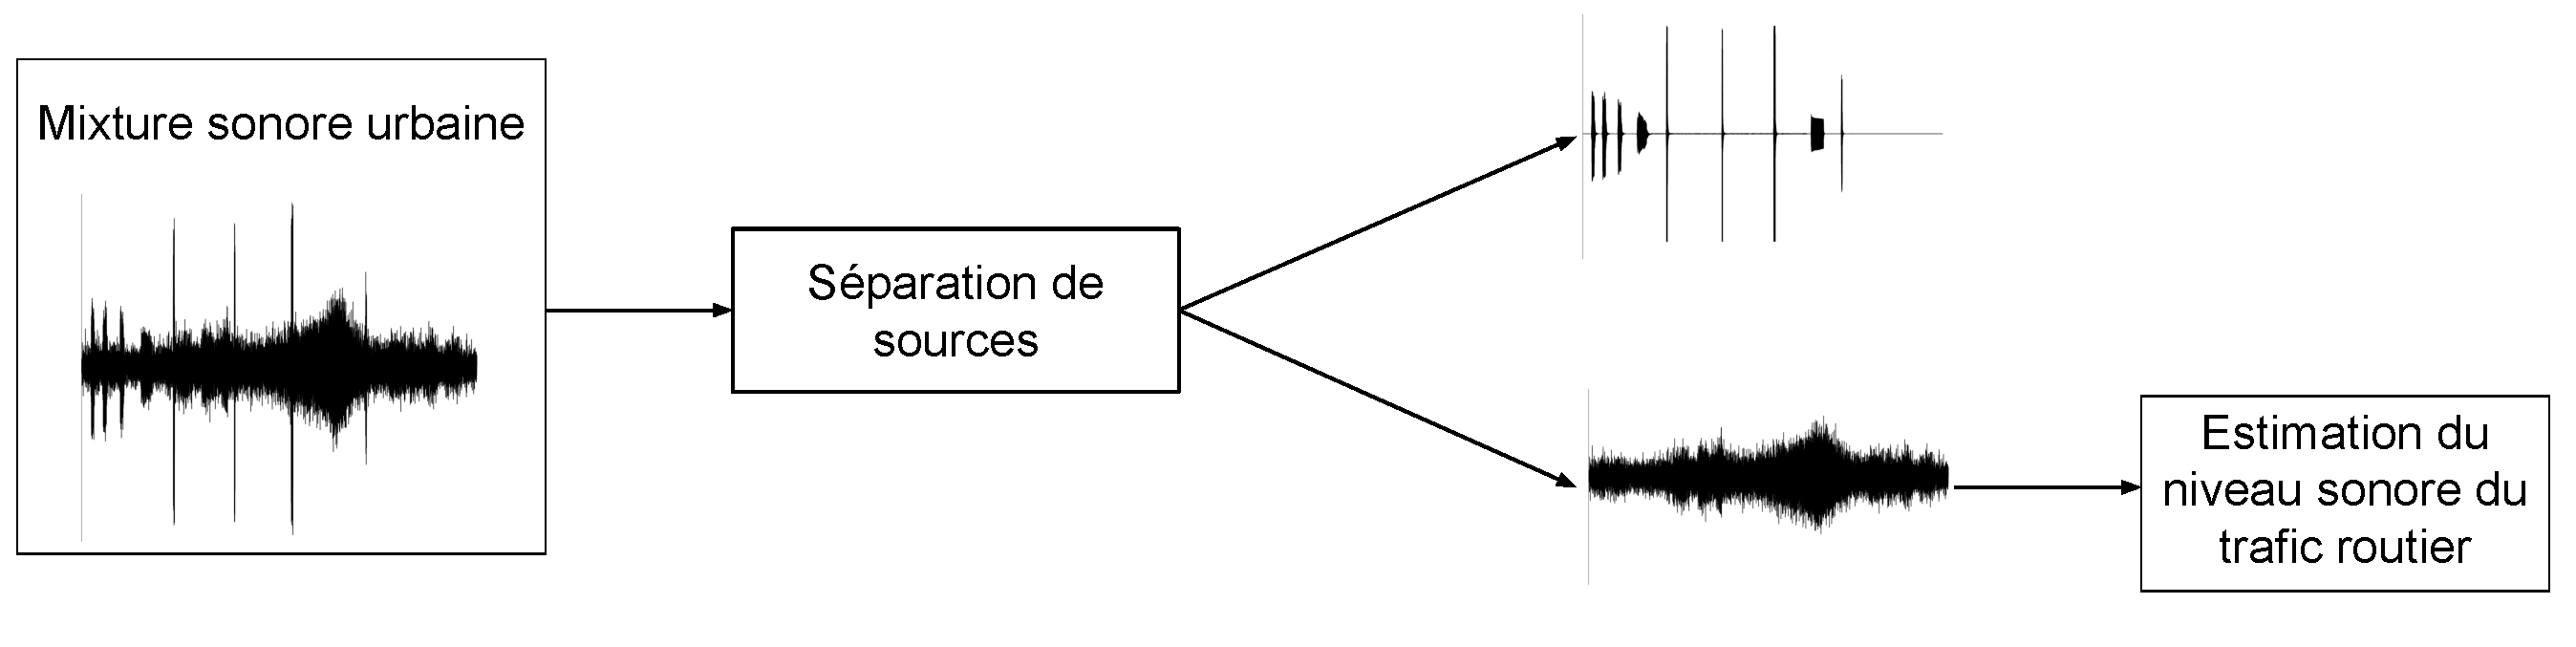
\includegraphics[width=\linewidth]{./figures/autres/schema_source_separation_FR.pdf}
\caption{Schéma de principe de la séparation de sources.}
\label{fig:separation_source_intro}
\end{figure}


En cela, la Factorisation de Matrices Non-négatives (abrégée NMF pour \textit{Non-negative Matrix Factorization} en anglais) \cite{lee_learning_1999} est l'approche retenue dans ces travaux car elle répond bien aux contraintes posées. Là encore, la NMF a été utilisée de très nombreuses fois pour des signaux contenant de la musique \cite{helen2005separation,fevotte_nonnegative_2009} ou de la parole \cite{wilson2008speech,schmidt2006single}. Plusieurs variantes à cette méthode ont été développées dont certaines sont implémentées dans ces travaux. Son application sur une telle source n'ayant jamais encore été réalisée, son fonctionnement, face à de tels environnements sonores,  nécessite d'être étudié. Également, dans le cadre de cette thèse, une nouvelle forme de NMF est proposée, appelée NMF \textit{initialisée seuillé}.
Afin d'étudier ses performances, la NMF n'est pas appliquée sur des enregistrements audio, car l'estimation faite du niveau sonore du trafic ne pourrait alors pas être comparée à une valeur exacte, mais sur des corpus de scènes sonores simulées. L'intérêt de ce procédé est qu'il permet de connaitre les contributions de chacune des sources dont la composante \textit{trafic}. La comparaison du niveau exact et estimé est alors possible.

Le propos de cette thèse est donc de proposer un protocole expérimental permettant d'évaluer la qualité d'estimation du niveau sonore du trafic routier par séparation de sources sur des mixtures simulées de scènes sonores urbaines. En cela, plusieurs approches de la NMF sont étudiées afin de définir l'approche optimale obtenant les erreurs d'estimation les plus faibles.\\

\ml{manque une liaison du genre. Pour cela il est necessaire d'introduire certains concepts comme bla bla bla}

Dans le premier chapitre, la définition formelle de l'objet d'étude, l'ESU, est réalisée. Ensuite, une revue des différentes méthodes visant à le caractériser est réalisée avec un exercice critique de leurs avantages et de leur limites. Au regard des observations faites, une proposition décrivant le protocole expérimental mis en place est alors faite.

Le second chapitre a pour objectif de décrire les différentes méthodes de séparation de sources qui peuvent être envisagées. Ces méthodes sont ensuite comparées selon le cahier des charges défini. La Factorisation en Matrices Non-négatives est alors la méthode retenue.
Son fonctionnement est présenté en détail dans le chapitre 3 selon les différentes méthodes d'apprentissage ou expressions des fonctions de coût. Ce chapitre introduit également la NMF \textit{initialisée seuillée}, élaborée durant les travaux de ce doctorat.

Le chapitre 4 est dédié à la réalisation de deux corpus d'évaluation composés de scènes sonores simulées et à la formation d'une base de données de sons isolés permettant de les composer.
Un premier corpus, nommé \textit{Ambiance}, est construit en mélangeant artificiellement une composante \textit{trafic}, dont le niveau sonore est calibré, avec d'autres classes de sons spécifiques. Ce premier corpus a pour vocation de tester la NMF, d'étudier son fonctionnement et ses performances face à des sons urbains.
Le second corpus, nommé \textit{SOUR} pour Scènes sOnores Urbaines Réalistes, se base sur des enregistrements audio qui ont été réalisés en ville.
L'annotation de ces enregistrements permet de définir une partition temporelle qui sert à la construction des scènes sonores. Le rendu obtenu est alors soumis à un test perceptif visant à évaluer le réalisme sonore des scènes simulées.

Les chapitres 5 et 6 sont ensuite dédiés à l'étude des performances de la NMF soumise aux deux corpus d'évaluation. Dans un premier temps, le fonctionnement de la NMF face au corpus \textit{Ambiance} est présenté en détail afin d'étudier le comportement de cette méthode face à de telles mixtures sonores. Les erreurs produites sur l'intégralité du corpus, selon le niveau sonore du trafic et selon chaque classe de son, sont présentées.
Les résultats sur le corpus de \textit{SOUR} sont ensuite exposés afin d'obtenir la forme optimale de NMF qui pourrait être implémentée dans des capteurs embarqués et utilisée comme outil de traitement du signal \textit{trafic}. Des méthodes d'optimisation sont alors proposées afin d'améliorer les performances de la NMF pour la tâche visée.

%\documentclass[twoside,openright,a4paper,11pt]{book}
%
%
\usepackage[utf8]{inputenc}
\usepackage[francais]{babel}
\usepackage[T1]{fontenc}

\addto\captionsfrench{\def\tablename{\textsc{Tableau}}}% pour avoir TABLEAU et pas TABLE dans les légendes des tableaux

%%%%%%% MISE EN PAGES %%%%%%
\usepackage{geometry}
\geometry{outer=2cm,inner=3cm,top=3cm}

\setcounter{tocdepth}{3}     % Dans la table des matieres
\setcounter{secnumdepth}{3}  % Avec un numero.
\usepackage{setspace}

\usepackage{fancyhdr}	% marge en haut et en bas
\pagestyle{fancy}

\fancyhead{}	% vide l'entête
\fancyfoot{} % vide le pied~de~page

\fancyhead[RO]{\leftmark}
\fancyhead[LE]{\rightmark}
\fancyfoot[C]{\thepage}	% numéro de page en bas au centre

\renewcommand{\headrulewidth}{0.4pt} % épaisseur du trait en haut
\renewcommand{\footrulewidth}{0.4pt} % épaisseur du trait en bas

\fancypagestyle{mypagestyle}{%
    \fancyhead{}	
    \fancyfoot{} 
    \fancyfoot[C]{\thepage}
    \renewcommand{\headrulewidth}{0.4pt} 
	\renewcommand{\footrulewidth}{0.4pt} 
}

\fancypagestyle{couvertureAbstract}{%
    \fancyhead{}	
    \fancyfoot{} 
    \fancyfoot[C]{}
	\renewcommand{\headrulewidth}{0pt} 
	\renewcommand{\footrulewidth}{0pt} 
}
%
\usepackage{layout}
\usepackage{tocbibind} % include tableofcontent in itself

%%%%%% PAGE DE GARDE %%%%%%

\geometry{outer=2cm,inner=3cm,top=3cm}
\usepackage[scaled]{helvet} % font used on cover (Helvetica)
\usepackage{eso-pic} % to set background picture
\usepackage{multicol} % for back cover (abstracts)
\usepackage{graphicx} % to include logos
\usepackage{tikz} % to compose background picture

% Colors (extracted from SPI's template)
\definecolor{boxcolor1}{rgb}{0.91373,0.92941,0.87451}
\definecolor{boxcolor2}{rgb}{0.94902,0.93333,0.91373}
\definecolor{boxcolor3}{rgb}{0.76078,0.87843,0.17647}
\definecolor{headercolor}{rgb}{0.94118,0.30980,0.17255}
\definecolor{namecolor}{rgb}{1.0,0.4,0.0}
\definecolor{titlecolor}{rgb}{0.19216,0.51765,0.60784}
% Also used: gray, teal (predefined by xcolor package, usually loaded by document class)

% Cover environment, to keep changes local
\newenvironment{cover}{%
  \fontfamily{phv}\selectfont % Select Helvetica font
  \pagestyle{empty} % No page number
}{
  \addtocounter{page}{-1}
  \cleardoublepage
}

% Macro for background common to front and back
\newcommand{\tikzBG}{%
  \path (0,0) rectangle (1,1);
  %TODO: You should adjust the bottom height of the following rectangle to fit your abstract's length
  \path [fill=boxcolor1] (.0571,.11) rectangle (.481,.963); 
  \path [fill=boxcolor2] (.4333,.697) rectangle (.9048,.7475);
  \path [fill=boxcolor2] (.4333,.7811) rectangle (.9048,.8316);
  \path [fill=boxcolor2] (.4333,.8687) rectangle (.9048,.9192);
  \path [fill=boxcolor3] (.0571,.7879) rectangle (.5762,.8316);
  \node[inner sep=0pt] at (0.2285,0.8788) [above left] {%
    
\includegraphics[height=.0707\paperheight,keepaspectratio]{./figures/logo/logo_unb.png}};
  \node[inner sep=0pt] at (0.6667,0.8788) [above right] {%
    
\includegraphics[height=.0808\paperheight,keepaspectratio]{./figures/logo/logo_ecn_color.png}};
  \node at (.0571,.8316) [above right,color=headercolor] {%
    \fontsize{29}{35}\selectfont\bfseries Th\`ese de Doctorat};
}

% Macro for repeated information (to avoid insconsistency)
%TODO: fill in with no formatting but desired case
\newcommand{\firstName}{Jean-Rémy}
\newcommand{\surname}{Gloaguen}
\newcommand{\thesisTitle}{Estimation du niveau sonore de sources d'intérêts au sein de mixtures sonores urbaines : application au trafic routier}

%%%%%%% SYMBOLES %%%%%
\usepackage{tipa}	% pour avoir l'accent concave
\usepackage{lmodern}	% pour les guillemets
\usepackage{gensymb}	% pour les degrés
\usepackage{enumitem}	% pour changer le symbole de l'item (\begin{itemize}[label=$\bullet$])

%%%%%%% EQUATION %%%%%%
\usepackage{amssymb}
\usepackage{amsmath}
\usepackage{fancybox}
\usepackage{xfrac}	% fraction de type "1/4"
\usepackage{cases}	% système équation
\usepackage[overload]{empheq}
\usepackage{bm}		% pour mettre en gras .
\usepackage{units} 	% x/y barre latérale pour les fractions
%
%%%%%%% FIGURE %%%%%%
\usepackage{subfigure}	% utiliser subfigure
\usepackage{float}	% utiliser H dans les figures
%
%%%%%% TABLEAUX %%%%%%
\usepackage{array,multirow,makecell}
%\addto\captionsfrench{\def\tablename{\textsc{Tableau}}}% pour avoir TABLEAU et pas TABLE dans les légendes des tableaux
\usepackage{colortbl} % pour avoir des lignes colorées dans les tableau
%\usepackage{slashbox} % pour les \backslashbox
%\usepackage{subcaption}
\usepackage{hhline}	% pour les lignes horizontales 
\usepackage{tabularx} % permet itemize dans les cellules
\usepackage{booktabs}
\usepackage{longtable}	% pour les tableaux longs

\newcolumntype{L}[1]{>{\raggedright\let\newline\\\arraybackslash\hspace{0pt}}m{#1}}
\newcolumntype{C}[1]{>{\centering\let\newline\\\arraybackslash\hspace{0pt}}m{#1}}
\newcolumntype{R}[1]{>{\raggedleft\let\newline\\\arraybackslash\hspace{0pt}}m{#1}}

%%%%% ALGORITHME %%%%%
\usepackage{algorithm}
\usepackage{algorithmic}

%%%%% BIBLIO %%%%%
\usepackage[fixlanguage]{babelbib}
\selectbiblanguage{french}
\usepackage{breakcites}	% pour couper les références en bout de ligne

%%%%% APPENDICES %%%%%%%
\usepackage[toc,page]{appendix}

%%%%%%%%%%%%%%%%%%%%%
\usepackage{url}	% gérer les adresses www.
\linespread{1.2}	% interligne

\cleardoublepage
%
%\begin{document}

\chapter{Connaitre l'environnement sonore urbain : de la prédiction à la mesure}
\thispagestyle{empty}

\section{Pourquoi s'intéresser aux environnements sonores urbains ?}

Au sein de l'Union Européenne, 70 $\%$ de la population, soit quasiment 340 millions d'habitants, vivent dans des zones urbaines \cite{europ-commission_data_2017}. 486 villes concentrent, chacune, plus de 100 000 habitants. En France, selon l'INSEE, c'est même plus de 84 $\%$ de la population qui vivent dans une zone urbaine, soit plus de 55 millions d'habitants. Cette concentration soulève de grandes questions autour de l'organisation de l'espace urbain afin d'offrir une qualité de vie acceptable aux citadins. En effet, avec de telles densités (environ 3000 habitants/km$^2$ et jusqu'à plus de 21 000  habitants/km$^2$ pour la ville de Paris, la plus dense de l'UE), plusieurs formes de pollutions viennent dégrader l'environnement urbain. Des sources de désagrément perçues par le citadin, le bruit est le phénomène qui provoque le plus de gène après la pollution de l'air. Ce bruit est le fruit des activités humaines, provenant essentiellement du transport qu'il soit routier, ferroviaire ou aérien \cite{zannin_characterization_2013}.\\

Selon un rapport de l'Organisation Mondiale de la Santé (OMS) \cite{who_burden_2017}, en Europe, près de 200 millions de personnes sont exposées quotidiennement à des niveaux sonores supérieurs à 55 dB($A$), soit 40$\%$ de la population. Près de 20 $\%$ atteignent même plus de 65 dB($A$) en journée et plus de 30 $\%$ sont touchées par un niveau sonore excédant 55 dB($A$) la nuit. En France, selon un rapport de l'ADEME \cite{europeens2016analyse}, ce sont 52 millions de personnes qui se disent affectées par le bruit et principalement le bruit issu du trafic routier. Plus de 7 millions d'individus y sont alors exposés à des niveaux supérieurs à 65 dB($A$) au quotidien et à plus de 55 dB($A$) la nuit.
Cette exposition quotidienne, à de tels niveaux, n'est pas sans conséquence pour l'Homme. L'impact sur l'organisme humain à l'exposition du bruit est observé et étudié depuis de nombreuses années \cite{ising1980health}. Parmi les effets possibles, les plus courants sont des troubles du sommeil \cite{pirrera2010nocturnal}, de la vigilance et de la concentration, l'augmentation du stress, de la pression artérielle et du rythme cardiaque \cite{babisch2008road, babisch2005traffic}. Selon le rapport de l'OMS, ce sont près de 8 millions de personnes en Europe qui sont affectées par des troubles du sommeil mais aussi 900 000 touchées par de l'hypertension. On estime aussi que 43 000 hospitalisations sont imputables au bruit dues à des pertes de vigilance et de concentration et jusqu'à 10 000 cas de morts prématurées par an. Cet impact sur la santé a alors un coût financier pour la société : en France, ce coût est estimé à plus de 11,5 milliard d'euros par an dont une grande partie (89 $\%$) est imputable au bruit du trafic routier \cite{europeens2016analyse}. 

De plus, si le bruit en ville impacte la vie des citadins, celui-ci se fait également ressentir auprès de la faune sauvage \cite{dutilleux_anthropogenic_2012, francis2009noise} leur causant également du stress ou en compliquant la communication et la reproduction entre les individus.\\

Le bruit, et une trop grande exposition à celui-ci, a donc un impact négatif sur les individus et sur leur environnement. C'est donc un enjeu de société dont les français ont conscience \cite{JNA2016etude}. 
Il est donc nécessaire et utile de s'intéresser aux environnements sonores urbains (ESU) afin de mieux estimer les sources sonores présentes, leur niveaux sonores et leur répartition.
%  Étant la source sonore la plus présente et la plus gênante, de nombreuses études prises se sont focalisées sur le bruit de trafic.

De nombreux modèles numériques existent afin de pouvoir prédire les niveaux sonores émis par du trafic routier \cite{quartieri2009review}, ferroviaire \cite{van2000railway} et aérien \cite{zaporozhets1998aircraft}.
À partir de ces modèles, est instaurée en 2002, la directive européenne 2002/49/EC dont le but est de mieux connaitre la répartition du bruit émanant de ces principales sources de bruit en ville ainsi que des Installations Classées pour la Protection de l'Environnement (ICPE) dans les agglomérations de plus de 100 000 habitants. Cette directive prévoit : 

\begin{itemize}
	\item d'évaluer l'exposition au bruit des populations basée sur des méthodes communes aux pays européens,
	\item d'informer les populations sur leur niveau sonore d'exposition et sur les effets du bruit sur la santé,
	\item de connaitre et de délimiter les zones bruyantes et les zones calmes.\\
\end{itemize}

Cette directive permet notamment la production de cartes de bruits stratégiques qui permettent de cibler les endroits où les niveaux sonores sont élevés afin de réaliser des aménagements qui permettront de les réduire (construction d'un mur anti-bruit, réduction de la vitesse, mise en place d'un revêtement sol particulier \dots).


\section{Réaliser des cartes du bruit en ville}
Mises à jours tous les 5 ans, les cartes de bruit résument, pour chaque source de bruit, les niveaux sonores globaux moyens pondérés $A$ sur 24h ($L_{DEN}$ pour \textit{Day-Evening-Night}) et durant la nuit ($L_N$) : 

\begin{equation}
L_{DEN} = 10\times\log \left(\frac{1}{24} \left(12\times10^{\frac{L_D}{10}}+4\times10^{\frac{L_E+5}{10}}+8\times10^{\frac{L_N+10}{10}} \right)\right)
\end{equation} 

avec $L_D$, $L_E$ et $L_N$, les niveaux sonores moyens à long terme pondéré A pour les périodes respectives 6h-18h, 18h-22h, 22h-6h (pouvant être changer suivant le rythme de vie du pays), 

\begin{subequations}
\begin{align}
L_D &= 10\times\log\left(\frac{1}{T} \sum_{t = 1}^{T}10^{\frac{L_{D_t}}{10}}\right),\\
L_E &= 10\times\log\left(\frac{1}{T} \sum_{t = 1}^{T}10^{\frac{L_{E_t}}{10}}\right),\\
L_N &= 10\times\log\left(\frac{1}{T} \sum_{t = 1}^{T}10^{\frac{L_{N_t}}{10}}\right).
\end{align}
\end{subequations}

Les niveaux $L_E$ et $L_N$ sont majorés respectivement de 5 dB($A$) et de 10 dB($A$) afin de pénaliser les plages horaires où la gêne occasionnée par le trafic est plus importante. La Figure \ref{fig:carto_nantes} résume, par exemple, le $L_{DEN}$ et le $L_N$ pour le bruit du trafic routier dans un quartier de la ville de Nantes.

\begin{figure}[t]
\centering
\subfigure[\label{fig:lden}]{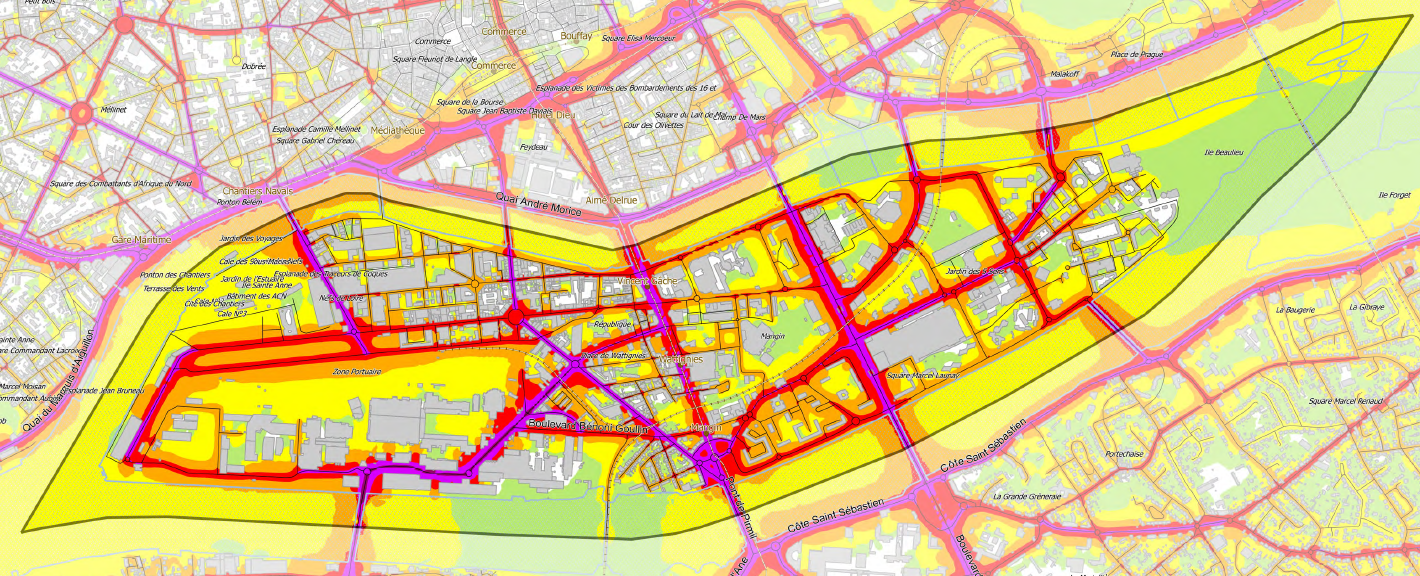
\includegraphics[width=0.85\linewidth]{./figures/cartographie/Lden_ile_Nantes.PNG}}
\subfigure[\label{fig:ln}]{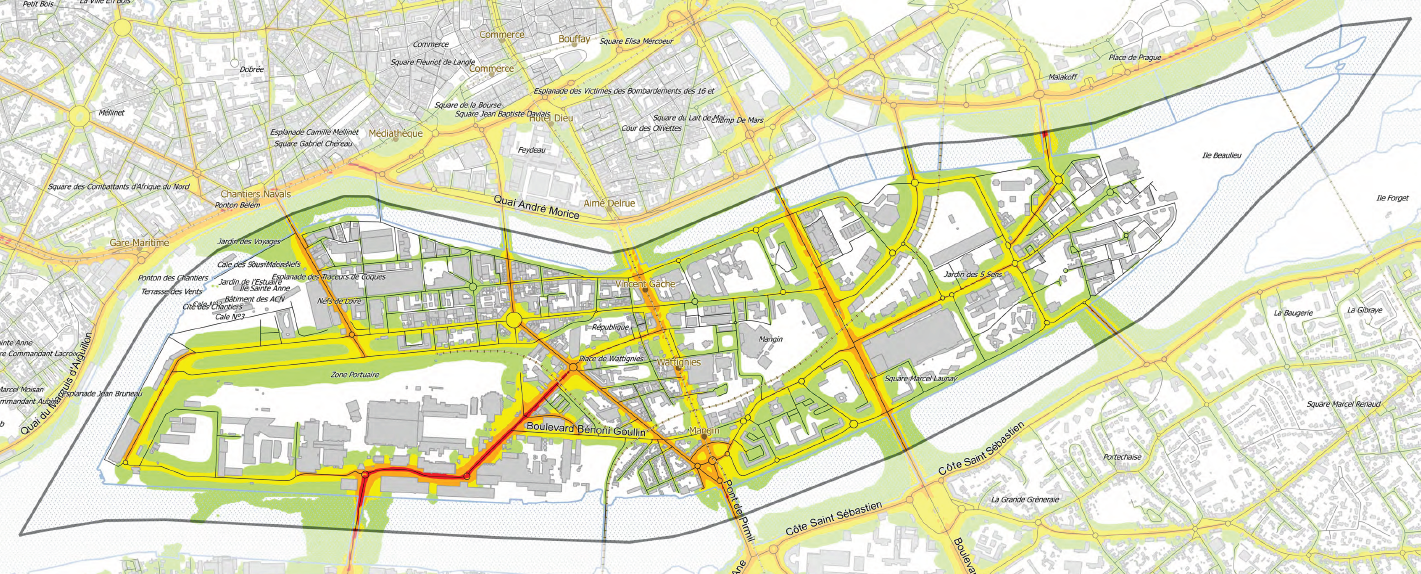
\includegraphics [width=0.7\linewidth]{./figures/cartographie/Ln_ile_Nantes.PNG}}
\caption{$L_{DEN}$ \subref{fig:lden} et $L_N$ \subref{fig:ln} de l'île de Nantes pour le trafic routier \cite{nantes_carte}.}
\label{fig:carto_nantes}
\end{figure}

Ces cartes sont issues de calculs numériques qui nécessitent de définir, comme données d'entrée, les caractéristiques des sources sonores et de l'environnement.  Dans le cas du trafic routier, cela revient à déterminer : 

\begin{itemize}
\item les vitesses moyennes des véhicules sur les portions de routes principales, 
\item les débits de véhicules (nombre de véhicules par tranche horaire \textit{Day, Evening, Night}), 
\item la composition du trafic (nombre de véhicules légers et de poids lourds).\\
\end{itemize}

Les lois d'émissions des sources sonores sont alors calculées. À partir de la topographie de la ville (architecture, revêtement du sol) et en obtenant les conditions météorologiques moyennes (température, vent), il devient possible de calculer, avec l'aide de modèles numériques de propagation acoustique, les niveaux sonores dans la ville produits par ces sources sonores. Plusieurs modèles existent comme le modèle NMPB-routes-2008 \cite{setra_prevision_2009-1, setra_prevision_2009-2},  CNOSSOS-EU \cite{CNOSSOS}, RSL-90\dots{} La génération des cartes peut être réalisée par des logiciels du commerce (comme Mithra, CadnaA ou Immi) qui font le choix d'utiliser un modèle de propagation parmi ceux existant. Actuellement, la méthode CNOSSOS-EU est l'approche la plus couramment utilisée à l'échelle de l'UE. Afin de déterminer, le nombre de citadins touchés par de forts niveaux sonores, les logiciels accompagnés d'un Système d'Information Géographique (SIG) sont ceux qui offrent le plus de possibilités. Un SIG est un outil informatique conçu pour stocker, analyser et manipuler plusieurs type de données spatiales et géographiques comme l'architecture des villes ou le nombre d'habitants présents. Leur utilisation permette de connaitre plus facilement le nombre de citadins exposés à des niveaux sonores \cite{murphy2011scenario}. Par exemple, le logiciel OrbisGIS\footnote{\url{http://orbisgis.org/}}, destiné à représenter de données spatiales, permet la réalisation de cartes de bruit à l'aide de l'ajout d'un plugin, \textit{NoiseModelling}, développé par \cite{fortin}. Un résumé des étapes est présenté en Figure \ref{fig:cartographie}.\\

\begin{figure}[t]
\centering
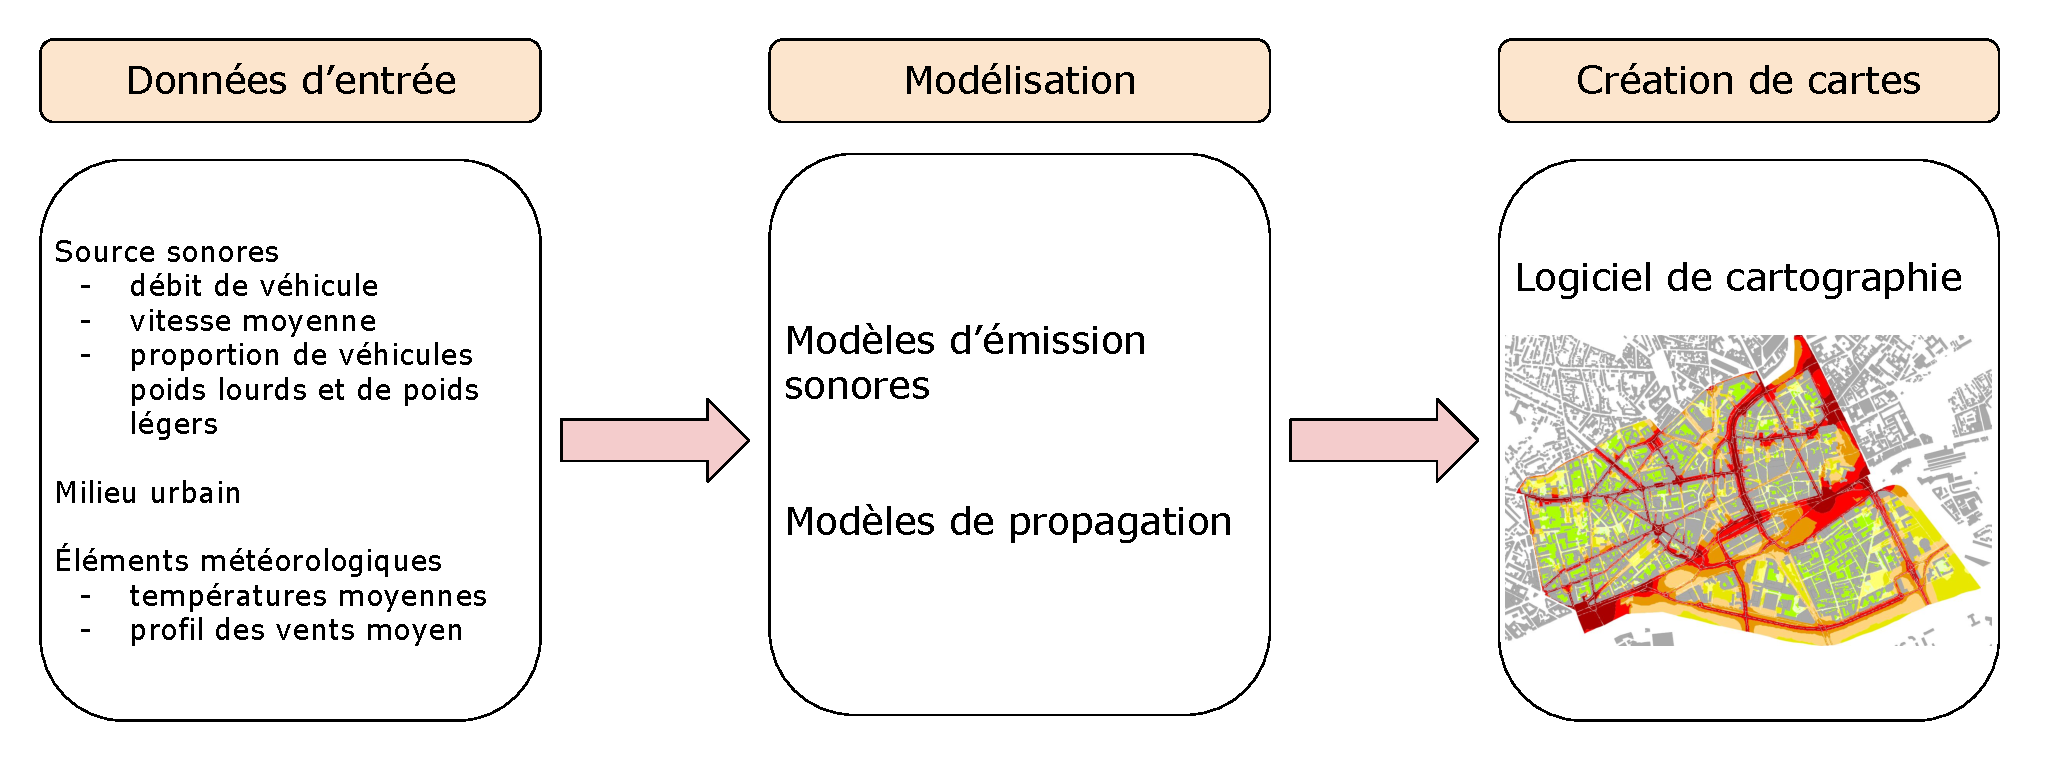
\includegraphics[width=.85\linewidth]{./figures/cartographie/cartographie.pdf}
\caption{Résumé des étapes menant aux cartes de bruit de trafic.}
\label{fig:cartographie}
\end{figure}


De nombreuses études basées sur l'étude du bruit en ville ou sur la réalisation de cartes de bruit dans des quartiers utilisent comme référence la directive européenne \cite{murphy_environmental_2006, murphy_estimating_2009, Eriksson_residential_2013}. Ces outils sont également utiles afin de tester différents scénarios d'aménagement (réduction de vitesse, changement de revêtements par exemple, construction d'immeuble \dots) \cite{murphy2011scenario,guedes2011influence}. Cependant, si l'utilité de ces cartes n'est pas remise en cause, chaque étape de la conception de ces cartes induit des incertitudes qui peuvent nuire à leur interprétation. 

\section{Limitations des modèles prédictifs de bruit de trafic}

\subsection{Incertitudes sur les données d'entrée}

La première source d'erreur est issue de l'estimation des données d'entrée à travers des valeurs moyennes qui induisent forcément des écarts types qui se propage par la suite aux étapes suivantes. 
Ensuite, le milieu urbain est évidemment simplifié pour éviter de complexifier et diminuer le temps de calcul. L'influence des plus petits mobiliers urbains est également mise de coté.
 

\subsection{Incertitudes des modèles physiques}

Ce type d'erreur est liée au choix de la méthode de calcul employée. Avant même la mise en place de la directive, Steele, dans \cite{steele_critical_2001}, avait comparé les méthodes de calculs (données d'entrée, type de cartographie, méthode de propagation des différents logiciels). Parmi cette diversité d'outils, l'auteur met en avant le problème, soulevé également par \cite{king_implementation_2011}, de la diversité des outils et des méthodes de calculs qui peuvent être employées. Plus récemment, Garg et Maji \cite{garg_critical_2014} réalisent une comparaison entre 8 méthodes de calcul (FHWA, CoRTN, RLS-90, ASJ RTN, Harmonoise, Son Road, Nord 2000n NMPB-Routes-2008) selon de nombreux points techniques : 

\begin{itemize}
\item modélisation des sources sonores (trafic, ferroviaire), 
\item condition de trafic (constantes, accélération/décélération, intersection\dots), 
\item modèle de propagation, 
\item prise en compte de la divergence géométrique, 
\item données d'entrées prise en compte, 
\item modélisation des effets de sol,
\item effets météorologiques,
\item effets de diffraction,
\item \dots  \\
\end{itemize}

Par exemple, la méthode RLS-90 est la seule à prédire la densité de trafic sur les axes routiers. La catégorisation des véhicules varie également entre les méthodes : dans la méthode Nord-2000, les véhicules sont divisés en 3 catégories selon leur poids alors que dans Son Road, il n'y en a que 2. Dans le cas du modèle de propagation, Harmonoise propose 3 méthodes (équation parabolique, tir de rayons et éléments de frontières) afin de s'adapter à différentes configurations là où, dans FHWA, c'est l'équation de propagation qui est résolue en prenant en compte les phénomènes comme l'absorption atmosphérique, les impédances des différentes surfaces rencontrées\dots{} Enfin les effets météorologiques sont pris différemment en compte selon les méthodes. La méthode NMPB suppose des conditions homogènes et favorables à la propagation. Dans Nord 2000, les gradients de température et de vent sont inclus alors que, dans les modèles Son Road et CoRTN, ces phénomènes ne sont pas pris en compte. L'ensemble des ces points amènent donc à des résultats divergeant entre les méthodes. 
Les auteurs concluent qu'il est toutefois difficile de déterminer un \og meilleur \fg{} modèle par rapport aux autres chacun ayant une approche différente. La validation de ces modèles par la mesure \textit{in situ} est complexe puisque de nombreuses sources sonores qui ne sont pas modélisées sont présentes en villes. 

Les premières cartes de bruits ont donc été établies sur des modèles différents. 
Afin de résoudre ces problèmes, la méthode CNOSSOS-EU \cite{CNOSSOS,kephalopoulos} a été développée. Même si elle présente certains défauts intrinsèques aux modèles prédictifs de bruit de trafic, elle permet d'harmoniser la construction des cartes de bruit des villes à l'échelle européenne permettant plus facilement leur comparaison. Dans le cas du trafic routier, la source sonore est décomposée selon 5 catégories de véhicule : légère, moyenne et lourde motorisation, 2 roues et autre. Cette dernière classe permet d'inclure, par exemple, les véhicules électriques. Les sources sonores sont décrites en prenant également en compte le bruit de roulement, de propulsion et les effets de l'accélération ou de décélération. 
La méthode de propagation choisie est celle des tirs de rayons. Entre la source et le récepteur, les chemins directs, réfléchis et diffractés sont considérés. En fonction des conditions atmosphériques relevées (température, vent), les atténuations dans les conditions favorables (à la propagation) et homogènes sont considérées. Les effets de sol (divisé en 8 catégories, du plus absorbant au plus réfléchissant), la divergence géométrique et l'absorption atmosphérique sont ensuite pris en compte. 

\subsection{Incertitudes liées à la modélisation numérique}

Les cartes de bruits étant simulées numériquement, des incertitudes apparaissent également liées à la modélisation et à la discrétisation du milieu urbain. Afin de limiter la durée des calculs, des techniques d'optimisation sont utilisées comme la discrétisation du milieu ou des sources de bruits. Par exemple, dans la méthode CNOSSOS, l'ensemble de l'émission sonore émise par une voiture est résumé en une source ponctuelle équivalente placé à 0,5 m du sol. Pour une route, considéré comme une source linéique de bruit, celle est discrétisée en un ensemble de sources ponctuelles alignées. Le choix de la distance entre ces points est alors un compromis à faire entre temps de calcul et la précision souhaitée. Toutefois la position de ces sources influe ensuite sur les phénomènes de réflexion et de diffraction et donc au résultat final. Enfin, entre ces sources ponctuelles, les niveaux sonores sont déterminés au moyen d'un calcul d'interpolation (linéaire, Kriging) qui viennent ajouter en plus des incertitudes \cite{van_leeuwen_noise_2015}. 
Également, toujours en vue de limiter la complexité des calculs, certains paramètres sont aussi ajustables comme le nombre de réflexion que subit un tir de rayon, ce qui a une influence directe sur l'établissement du champs diffus. 

\subsection{Incertitudes liées à la restriction d'informations}

Une des principales limites des modèles de bruits en ville est la restriction d'informations qu'elles proposent : 2 niveaux sonores, $L_{DEN}$ et $L_N$, par source de trafic, sont estimés et mis à jours seulement tous les 5 ans. Cependant, le trafic routier, ferroviaire et aérien varient aussi bien à l'échelle de l'année, d'une journée ou même d'une heure \cite{lv2015traffic}. 
L'utilisation de modèles dynamiques de trafic, couplé aux modèles d'émissions sonore  \cite{can2010traffic}, n'est actuellement pas destiné à la cartographie des ESU mais à l'étude des interactions entre les véhicules et à leur cinématique. 
Enfin, les modèles prédictifs de bruit ne sont actuellement pas validés \textit{in situ}. En effet, ces modèles de bruits actuel ne permettent d'estimer que les niveaux sonores des sources relatifs au trafic alors que le milieu urbain est composé d'une multitude de sources sonores qui ont une influence sur l'Environnement Sonore Urbain (abrégé ESU dans la suite du document) perçu par le citadin. De précédentes études \cite{Mioduszewski, zannin_characterization_2013} ont observé des différences significatives entre les niveaux sonores mesurés et calculés. Si ces différences peuvent provenir des inexactitudes générées par la simulation, une part de ces écarts proviennent de la présence d'autres sources sonores qui sont prises en comptes dans les mesures mais qui ne sont pas modélisées.\\ 

\section{Vers la modélisation d'autres sources sonores ?}

De nombreuse études se sont intéressées à l'étude des ESU à travers la perception qu'en ont les citadins (\cite{brocolini_measurements_2013},  \cite{hong2013designing}). La plupart de ces études définissent des grandeurs acoustiques (\textit{activité}, la \textit{clarté, l'évolution temporel, l'occupation spatiale}\dots) qui sont évalué sur des échelles de taille variables limités par des qualificatifs (respectivement \og monotone/varié \fg{}, \og brouhaha/distinct \fg{}, \og figée/évolutive \fg{}, \og peu présente/très présent \fg{} \dots) \cite{raimbault2003ambient}.
Une des difficultés est alors de lier les évaluations de ces grandeurs, lié au ressenti des gens, à des indicateurs physiques mesurables avec des instruments de mesures. 
Pour cela, certaines études se sont intéressées à corréler ces évaluations à des indicateurs physiques.
Dans \cite{torija2013application}, le paysage sonore est décrit, à partir d'écoutes réalisées en laboratoire, par 14 indicateurs physiques dont le facteur crête (rapport du niveau sonore maximum sur le niveau sonore équivalent à 15 minutes), le niveau sonore pondéré $A$ des signaux contenant une réponse impulsionnelle ou les niveaux sonores des bandes de tiers d'octave de 125 Hz et 16 kHz. 
Dans \cite{hong2014soundscape}, des cartes du paysage sonore urbain sont réalisées, à l'aide d'un logiciel SIG, à partir de l'évaluation perceptive de la présence du trafic, des sons technologiques, des sons humains et des sons naturels ainsi que de l'évaluation du paysage sonore et de l'environnement urbain. Ces évaluations sont complétées par un seul indicateur physique, le niveau sonore équivalent pondéré $A$, $L_{A,eq}$. Cette étude révèle que le bruit de trafic perçu est corrélé au $L_{A,eq}$ alors que les sons naturels (sifflement d'oiseaux, bruit de fontaine) ne le sont pas (corrélation négative). Dans \cite{aumond2017modeling}, c'est la notion d'agrément sonore qui est défini (ESU plaisant ou déplaisant) à partir de deux modèles : l'un physique et l'autre perceptif. Le modèle physique est basé sur des indicateurs physiques tels que le niveau sonore fractile $L_{50}$ dans la bande de tiers d'octave de 1 kHz ainsi que la variation normalisée en temps et en fréquence des bandes de 500 Hz et de 4 kHz. Le modèle perceptif est, quant à lui, établit à partir du niveau sonores globale et du temps de présence de plusieurs source sonore spécifiques : trafic, voix, et oiseaux. 
Ce modèle perceptif est intéressant car il ne lie pas la perception du citadins qu'à des indicateurs acoustiques mais avec, également, les temps de présence du trafic, des oiseaux et de la voix. Pour les estimer, l'utilisation des modèles prédictifs de bruit de trafic se révèlent donc insuffisants pour pouvoir compléter ce modèle perceptif en cela que la présence des oiseaux et de la foule sont inconnues. Or, leur modélisation \cite{hayne2011prediction} \cite{} ou celle d'autres sources, comme les fontaines \cite{watts2009measurement}, n'est, pour l'instant, que très peu étudiée.
De plus, la localisation de certaines de ces sources dans l'espace urbain reste difficile. En effet, les éléments trafic se concentrent sur des axes qui leur sont dédiés, l'estimation de leur débit est alors réalisable. Certaines sources sonores, comme les fontaines ou les cloches d'une église, étant fixes, sont aussi faciles à localiser. Mais les sources sonores, comme la foule et les oiseaux, sont plus difficiles à déterminer car plus mobiles et parcimonieuses. C'est donc plus par une approche statistique qu'on détermine les positions où ces sources sont le plus susceptibles de se trouver (sur des places ou sur les trottoirs pour les piétons, dans les parcs pour les oiseaux).\\

En conclusion, l'utilisation de modèles prédictifs existants ne permettent pas définir correctement les ESU et leur perception dans son ensemble. Ces modèles sont dédiés à un ensemble trop restrictif de sources sonores et présentent de nombreuses incertitudes. Afin de considérer l'ensemble des sources et des évènements sonores présents en ville et de compléter l'apport des modèles prédictifs, une autre approche est envisagée, basée sur la réalisation de mesures et d'enregistrements sonores. 

\section{Utilisation de mesures acoustiques}

À l'heure de l'émergence de l'\textit{Internet des choses} (ou \textit{Internet of Things} en anglais) \cite{zanella2014internet} et de la \textit{Smart City} \cite{chourabi2012understanding}, de nombreuses villes s'équipent actuellement en réseaux de différents types de capteurs disséminés dans le milieu urbain afin de mieux contrôler, en temps réel, de nombreux aspects de la ville : distribution d'énergie, gestion des transports, de l’eau ou des déchets. L'objectif étant alors d'optimiser le fonctionnement de la ville afin d'améliorer la qualité de vie des citadins.
L'intégration de capteurs acoustiques dans ces réseaux est alors une voie pour étudier les ESU dans leur globalité. Plusieurs approches ont été étudiées pour réaliser ces mesures à l'aide d'un ou de multiples capteurs, à partir de mesures fixes ou mobiles.

\subsection{Déploiement de réseaux de capteurs fixes}

Un des premier déploiement de capteurs consiste à installer à des positions définies des microphones professionnels pour une durée finie. Cette approche permet ainsi d'avoir accès aux variations à long terme des niveaux sonores à l'emplacement des microphones dont la position est connue et choisie spécifiquement. Un réseau de capteurs développé depuis plusieurs année est celui de la ville de Paris, géré par BruitParif, à travers le projet RUMEUR \cite{mietlicki2012innovative}, en région parisienne, qui existe déjà depuis plusieurs années où des réseaux de microphones sont déployés afin d'évaluer l'ESU en région parisienne. Un site internet\footnote{\url{http://rumeur.bruitparif.fr/}} est mis à disposition pour avoir un aperçu complet des mesures réalisées sur les nombreux sites. 
À une moindre échelle, plusieurs études se sont également intéressées à la réalisation de mesures de longue durée au sein de la ville. 
Dans \cite{Mioduszewski}, 40 microphones sont placés isolément à travers la ville de Gdansk en Pologne pour une durée d'un an afin de valider la cartographie de bruit. Dans \cite{zannin_characterization_2013}, 58 points de mesures qui sont déployés dans un campus universitaire de la ville de Curitiba au Brésil afin d'étudier son environnement sonore. Mais le coût de ces capteurs et leur maintenance restent élevés et leur déploiement dans un réseau dense à l'échelle d'une ville ou d'un quartier devient alors prohibitif. Grâce au développement de capteurs acoustiques à bas coûts \cite{van2010use}, il devient, aujourd'hui, envisageable de déployer un plus grand nombre de microphones à travers les villes pour des durées de mesures plus longues au détriment, certes, des performance individuelle de chaque capteur \cite{aumond2017study}. 

\begin{figure}[t]
\centering
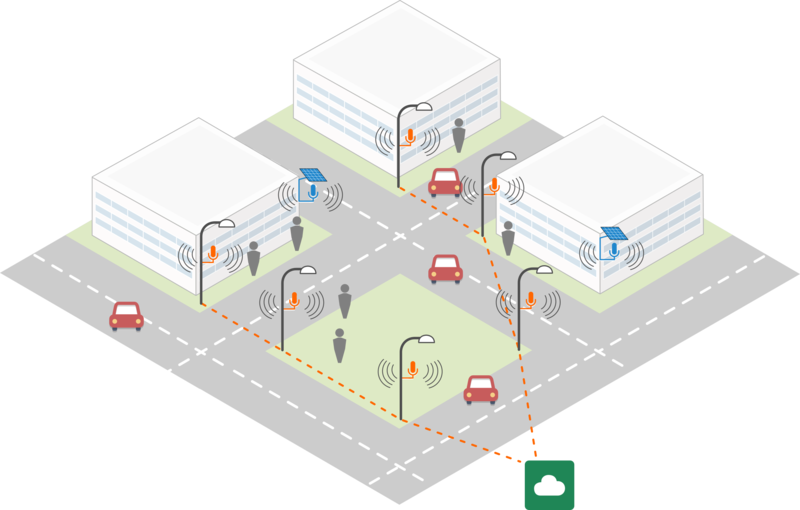
\includegraphics[width=0.8\linewidth]{./figures/cartographie/reseau_mesure.png}
\caption{Schéma d'un réseau de capteurs fixes}
\label{fig:reseau_capteur}
\end{figure}

\`A l'heure actuelle, plusieurs projets étudient la mise en place et la faisabilité de telle installation comme le projet européen DYNAMAP \footnote{\url{http://www.life-dynamap.eu/}} \cite{dynamap_2016}. Ce projet a pour objectif de développer un système de cartographie de bruit dynamique basé sur des réseaux de capteurs à bas coûts installés en ville. Une application de ce projet a déjà été réalisée dans deux villes tests, Milan et Rome \cite{bellucci_life_2017}. 

Le principe de leur approche est d'ajuster les cartes de bruits simulées à partir des différences obtenues entre les niveaux sonores mesurés aux stations et les niveaux sonores calculés à ce même point par les modèles prédictifs. Pour limiter le coût d'un tel déploiement, le nombre de microphones est réduit en les installant à des emplacements spécifiques représentatifs des différents scénarios possibles de trafic routier (homogénéité du trafic, type de revêtement, type de trafic\dots) \cite{zambon2017life}.
Le projet SONYC \footnote{\url{https://wp.nyu.edu/sonyc/}} à New-York dédie son réseau de capteurs à la surveillance de la pollution sonore et au développement d'outils de traitement du signal afin de décrire l'ESU par l'étude des sources présentes \cite{mydlarz2017noise}. Dans \cite{salamon2015unsupervised}, les auteurs classifient les évènements sonores à partir de leur base de données de sons, UrbanSound8k \cite{salamon_dataset_nodate}, avec, en tant que classifieur, un algorithme de k-moyenne sphérique.
Enfin, le projet CENSE\footnote{\url{http://cense.ifsttar.fr/}} vise à développer un réseau de capteurs dans la ville test de Lorient afin d'agréger les données simulées du niveaux sonores du trafic avec des mesures réalisées en ville par ce réseau en vue, là encore d'améliorer la cartographie du bruit de trafic. L'approche est différente de DYNAMAP, puisqu'ici l'étude se restreint à l'échelle de plusieurs quartiers de la ville afin d'avoir un réseau de capteurs dense. La mise à jour des cartes est faite à l'aide de techniques d'assimilation de données en vue de compléter les cartes de bruits prédites avec les mesures. 
Ces méthodes d'assimiliation sont notamment utilisés dans le domaine des sciences géophysiques et consistent à modifier une estimation émises par un modèle prédictif à partir de données mesurées \cite{wu2008comparison}.
Le projet s'intéresse également à la perception des citadins des ESU aux travers de questionnaires et des mesures réalisées par ce réseau de capteurs.
 
L'installation de tels réseaux de capteurs nécessite de gérer de nombreuses problématiques techniques comme la disposition des microphones, leur maintenance, la transmission des mesures, leur alimentation\dots{} Une des principales difficultés est celle de de la spatialisation des mesures et de la surface couverte par ces mesures : un réseau distribué selon un maillage dense permettra une bonne représentation de l'espace mais coutera cher à installer et à maintenir alors qu'une faible densité de capteurs sera moins onéreuse mais apportera moins d'information et nécessitera des interpolations entre les mesures, sources d'incertitudes.
Toutefois, la réalisation de mesures acoustique en ville n'est pas nécessairement obligée d'être réalisée via un réseaux de capteurs fixes. D'autres pistes sont également explorées.

\subsection{Mesures mobiles}
En parallèle des réseaux fixes, la mesure mobile est une voie envisagée. Elle consiste à réaliser des mesures acoustiques en plaçant le microphone sur un support mobile (piéton, cycliste, voiture, bus). L'avantage de cette méthode par rapports aux capteurs fixes est sa capacité à pouvoir couvrir plus facilement une plus grande surface urbaine à moindre coût. Les mesures mobiles sous-entendent deux manières d'être réalisées : soit le microphone réalise sa mesure sur un support mobile qui se déplace en même temps \cite{alsina-pages_design_2016}. Dans ce cas, un traitement du signal doit être effectué pour prendre en compte le bruit émis par ce support, soit le support permet de déplacer le microphone pour faire ensuite des mesures fixes \cite{manvell2004sadmam} ce qui simplifie la tâche mais qui nécessite plus de temps pour couvrir une surface similaire par rapport aux mesures faites sur un support mobile. 
L'inconvénient de ces méthodes est qu'elle ne permettent pas la réalisation de mesures à long terme et donc de ne pas pouvoir estimer l'évolution temporelle des niveaux sonores en un point donné au cours du temps. 
En conséquence, plusieurs travaux se sont intéressés à l'agrégation des mesures mobiles à des mesures réalisées par des stations fixes.
\cite{morillas2014uncertainty} s'intéresse aux incertitudes sur l'estimation des niveaux sonores estimés suivant le nombre de points ou de jours de mesures. Dans \cite{can2014measurement}, la prise en compte de mesures mobiles pour compléter des stations fixes est comparé à des méthodes d'interpolation (méthode de Kriging , pondération inverse de la distance). Il en résulte que l'apport des mesures mobiles diminue l'erreur produite par rapport aux méthodes d'interpolation en cela qu'elles permettent d'apporter plus d'informations quant aux variations spatiales du niveau sonore (rues calmes peu fréquentées, rues très passantes, aux abords d'intersections\dots) ce que ne permet pas une méthode d'interpolation numérique. \cite{aumond2018kriging} 

\begin{figure}[t]
\begin{center}
    \begin{minipage}[t]{0.3\textwidth}
        \centering
        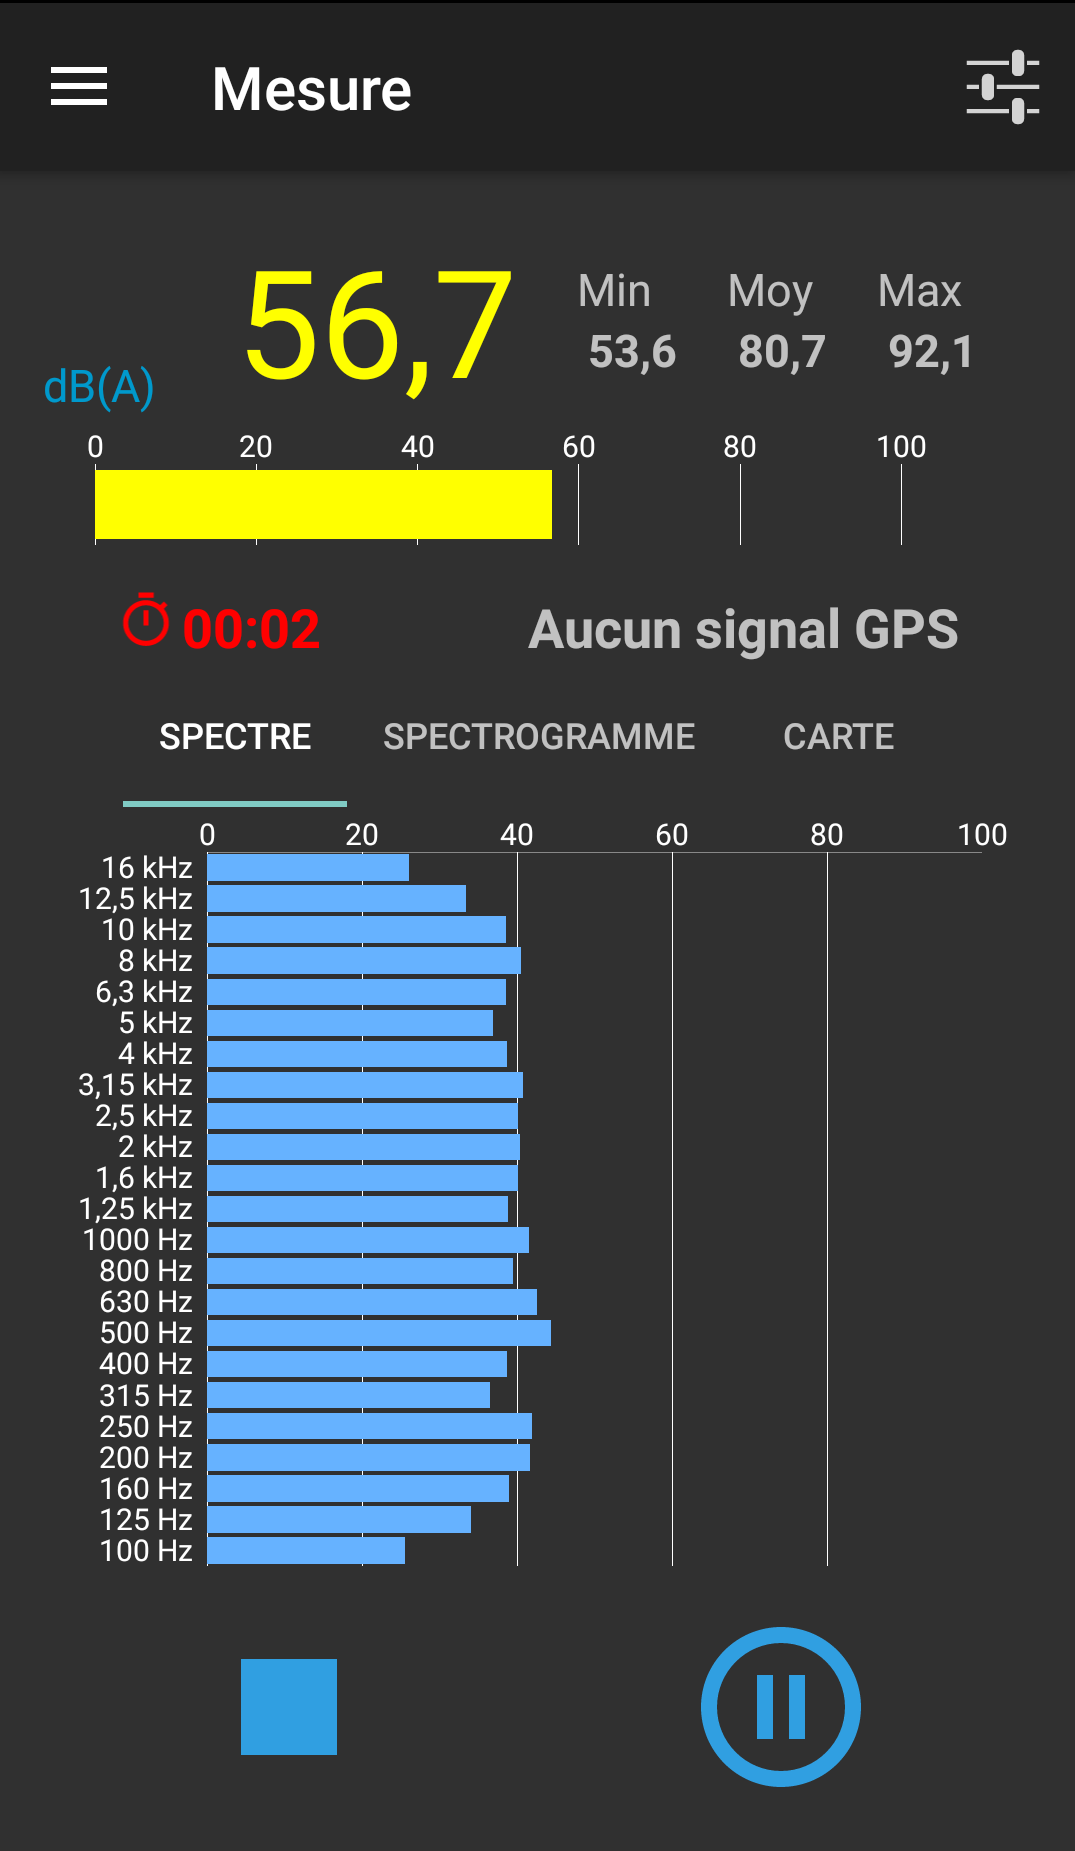
\includegraphics[width=0.9\textwidth]{./figures/autres/noiseCapture1.png}
    \end{minipage}
    \begin{minipage}[t]{0.3\textwidth}
        \centering
        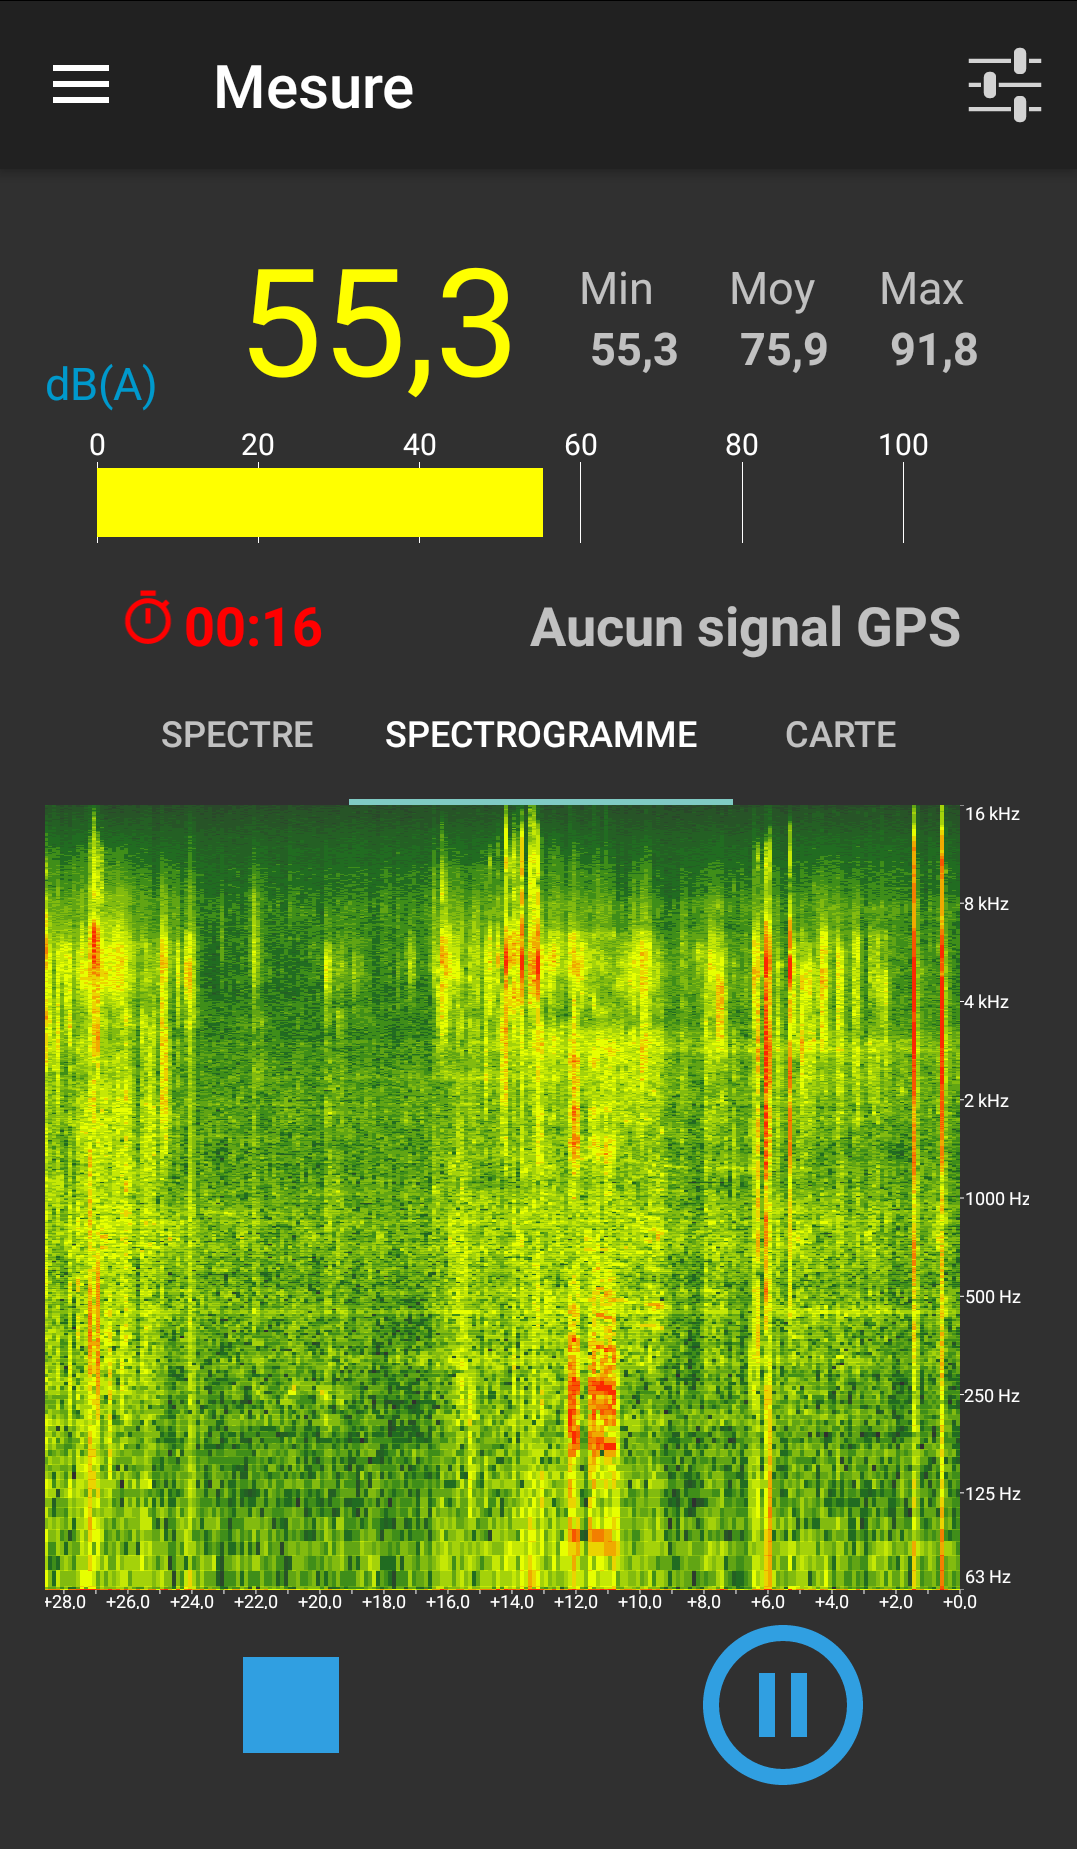
\includegraphics[width=0.9\textwidth]{./figures/autres/noiseCapture3.png}
    \end{minipage}
    \begin{minipage}[t]{0.3\textwidth}
        \centering
        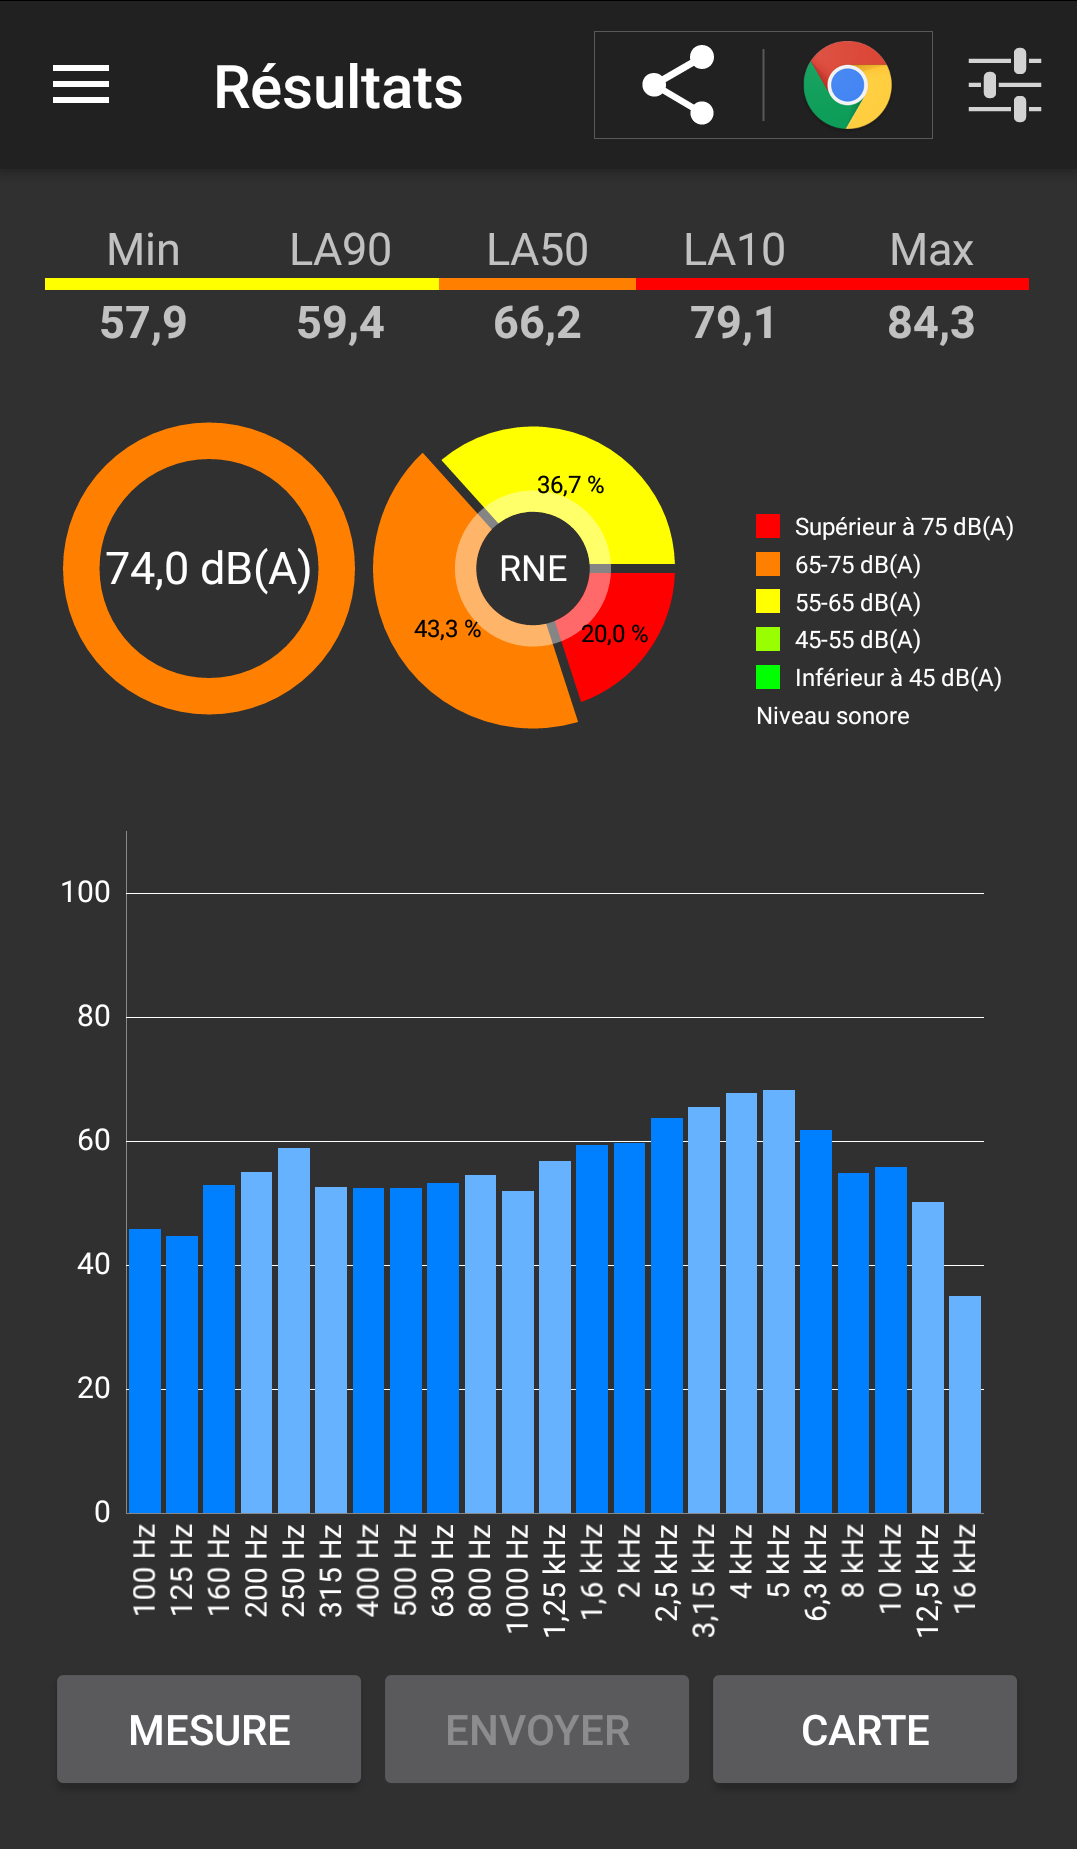
\includegraphics[width=0.9\textwidth]{./figures/autres/noiseCapture2.png}
    \end{minipage}
    \caption{Captures d'écran de l'application \textit{NoiseCapture}}
\end{center}
\end{figure}

\subsection{Mesures participatives}

Enfin, la participation des citadins peut être sollicitée aux travers de mesures participatives. Celles-ci peuvent se réaliser en équipant les personnes de dispositifs spécifiques \cite{aumond2017study} ou bien à partir d'applications développées pour smartphones. Profitant de la démocratisation de ces appareils et de l'augmentation de leurs performances, ces applications leur permettent d'avoir un dispositif suffisamment performant pour mesurer les niveaux sonores. Cette approche permet surtout d'obtenir un plus grand nombre de mesures qui ont le plus souvent une distribution spatiale et temporelle plus aléatoire mais qui sont aussi effectuées moins régulièrement. L'utilisation de ces mesures est toutefois encore sujet à caution puisque de nombreux problèmes sont encore à résoudre comme la calibration et la prise en compte des performances des microphones dans les faibles et forts niveaux sonores ou bien qualité de la réalisation de la mesure faite par l'utilisateur\dots{} Dans ce cas, le traitement statistique des résultats est primordial afin de détecter les mesures incongrues pour ne pas les considérer \cite{guillaume2016noise}. Plusieurs applications ont été dévelopées comme \textit{NoiseSpy} \cite{kanjo_noisespy_2010} ou \textit{Ambicity} \cite{ventura2017estimation}. On peut également relever le projet \textit{Noise Planet}\footnote{\url{http://noise-planet.org}} qui a pour objectif de proposer un outil libre et gratuit pour évaluer le bruit de l'environnement sonore. Il comprend une application pour smartphone, \textit{NoiseCapture} \cite{guillaume2016noise}, qui permet, là aussi, à l'utilisateur d'évaluer les niveaux sonores l'entourant tout en ayant la possibilité de décrire, à l'aide de mots-clés prédéfinis, les sons présents et l'ambiance sonore de la scène. La géo-localisation et les mesures sont ensuites collectées puis traitées pour produire des cartes de bruits, publiées en ligne (voir Figure \ref{fig:carte_noiseModelling}). En plus de collecter plus de données, ces applications permettent également de sensibiliser le citadin à son environnement sonore.\\ 

\begin{figure}[t]
\centering
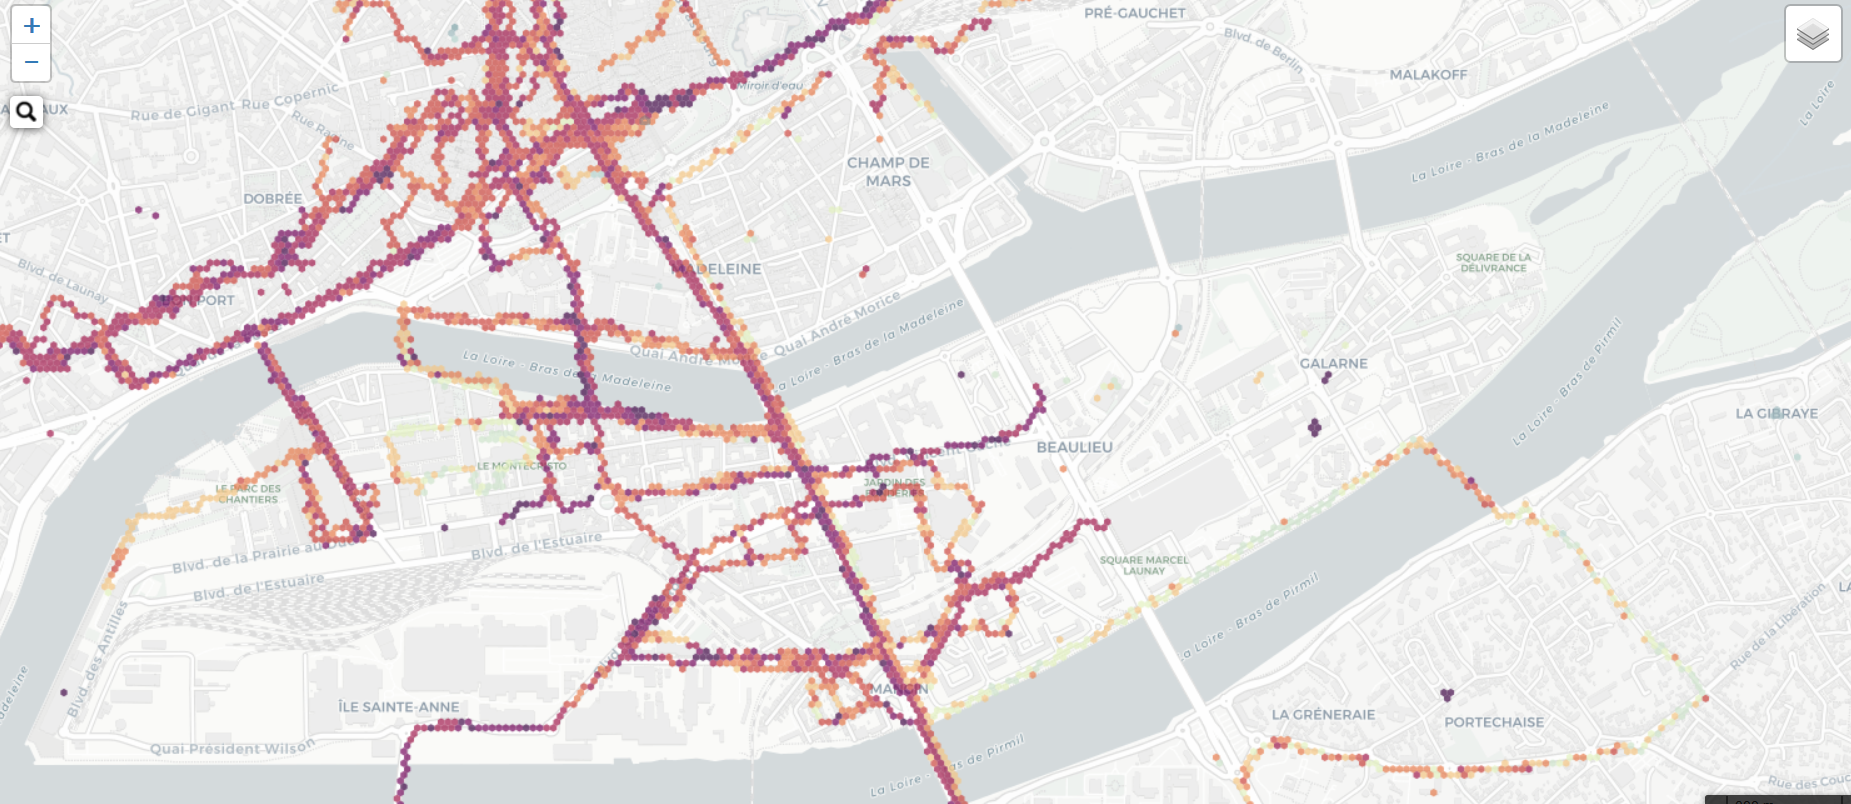
\includegraphics[width=0.7\linewidth]{./figures/cartographie/noise_modelling.PNG}
\caption{Carte de l'ESU de l'île de Nantes mesurée par l'application \textit{NoiseCapture}  (relevée le 22/03/2018)}
\label{fig:carte_noiseModelling}
\end{figure}


\section{De l'extraction d'informations des mesures}

Là où l'approche par modèles prédictifs suppose l'utilisation de modèles d'émissions sonores pour chaque source, l'utilisation de mesures acoustiques, dans le cadre de l'étude des ESU, permettrait : 

\begin{itemize}
\item d'estimer la contribution \textit{in situ} du trafic routier pour, au minimum, valider les modèles des prédiction de bruit de trafic ou, au mieux, pouvoir estimer le niveau sonore du trafic plus précisément et finement,
\item de considérer l'ensemble des sources sonores présentes afin de caractériser les ESU dans leur globalité,
\item et de s'orienter vers la cartographie multi-sources par l'estimation des contributions de sources sonores spécifiques pour ainsi mieux considérer la perception du citadin.\\
\end{itemize}

Toutefois, comme tout signal mesuré, il est nécessaire de disposer d'outils adaptés afin d'y déterminer les informations utiles. En effet, l'ESU est un milieu complexe composé d'une multitude de sources variées (trafic routier, voix, oiseaux, klaxon, bruit de pas\dots). Ces sources ont des allures temporelles différentes parfois brèves (le retentissement d'un klaxon) ou longues (le passage d'une voiture) ainsi que des allures spectrales variées (dans les basses fréquences pour le trafic, dans les hautes fréquences pour le sifflement des oiseaux), voir Figure \ref{fig:sourceUrbain}. L'ensemble de ces sources est aussi susceptible d'être généré simultanément. La création d'outils adaptés à cet environnement pour reconnaitre ou détecter des sources spécifiques n'est donc pas triviale. Par exemple, dans le cas du trafic routier, s'il existe des endroits où celui-ci est prépondérant sur les autres sources sonores (périphérique, grand boulevard), il peut l'être moins dans d'autres lieux (dans des rues calmes, au niveau de parc) où ce sont d'autres sources sonores qui sont majoritairement présentes (voix, oiseaux \dots). Dans \cite{Mioduszewski}, la réalisation de mesures par 40 stations fixes durant 1 an révèle que les niveaux sonores mesurés sont supérieurs à ceux estimés par les modèles prédictifs de bruit de trafic routier. Une part de cette surestimation provient de la prise en compte des bruits qui ne sont pas relatifs au trafic  mais aussi des modèles prédictifs qui ne permettent pas de considérer l'ensemble des variations sonores des véhicules. Ses travaux révèlent donc la nécessité de générer un outil adapté à l'étude des mesures et enregistrements faits en villes pour y extraire les contributions et les niveaux sonores des sources présentes en villes. Considérer l'ensemble des mesures et des enregistrements réalisés en ville sans distinction particulière entre les sources peut donc mener à de mauvaises estimations du temps de présence ou de son niveau sonore et donc à de mauvaises interprétations.\\

\begin{figure}[t]
\centering
\subfigure[\label{fig:sourceUrb1}]{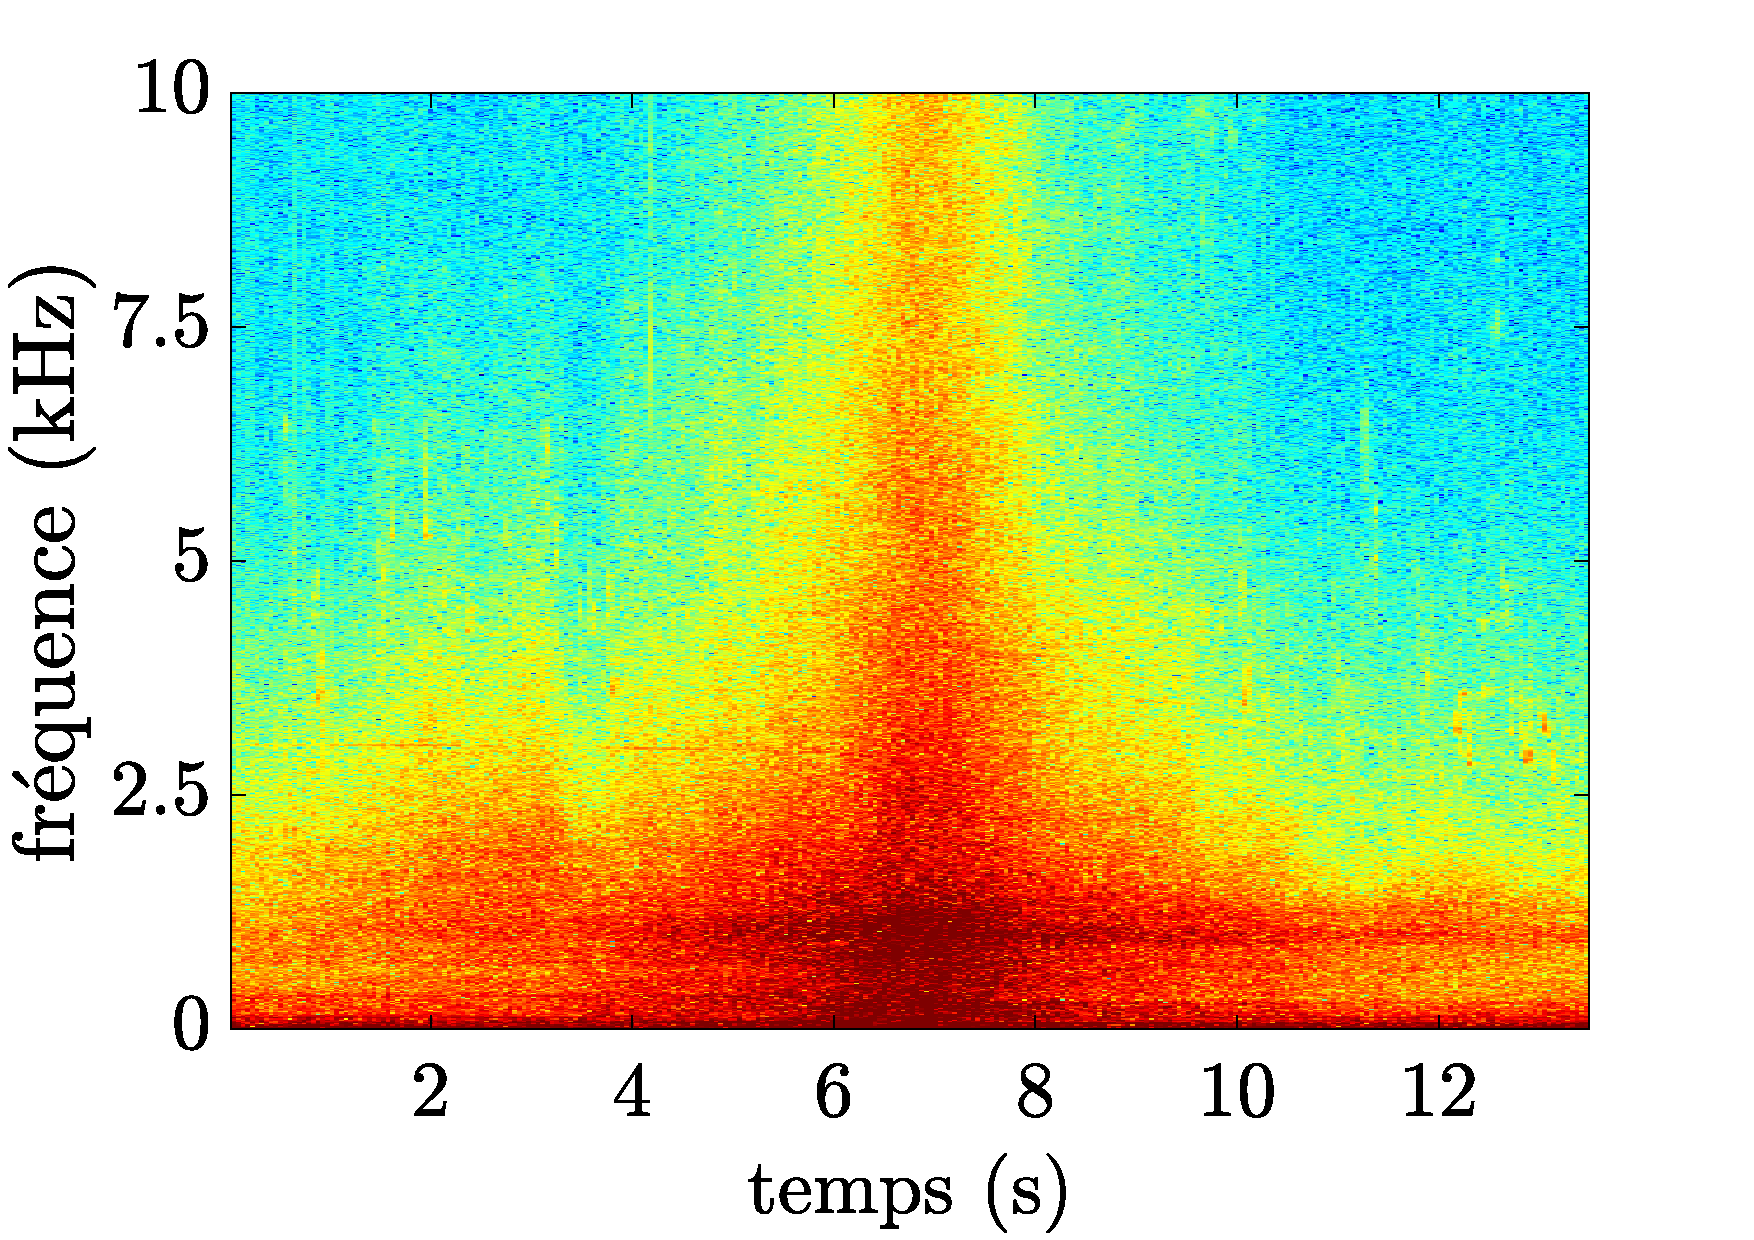
\includegraphics[width=0.4\linewidth]{./figures/autres/sourcesUrbainesCar.pdf}}
\subfigure[\label{fig:sourceUrb2}]{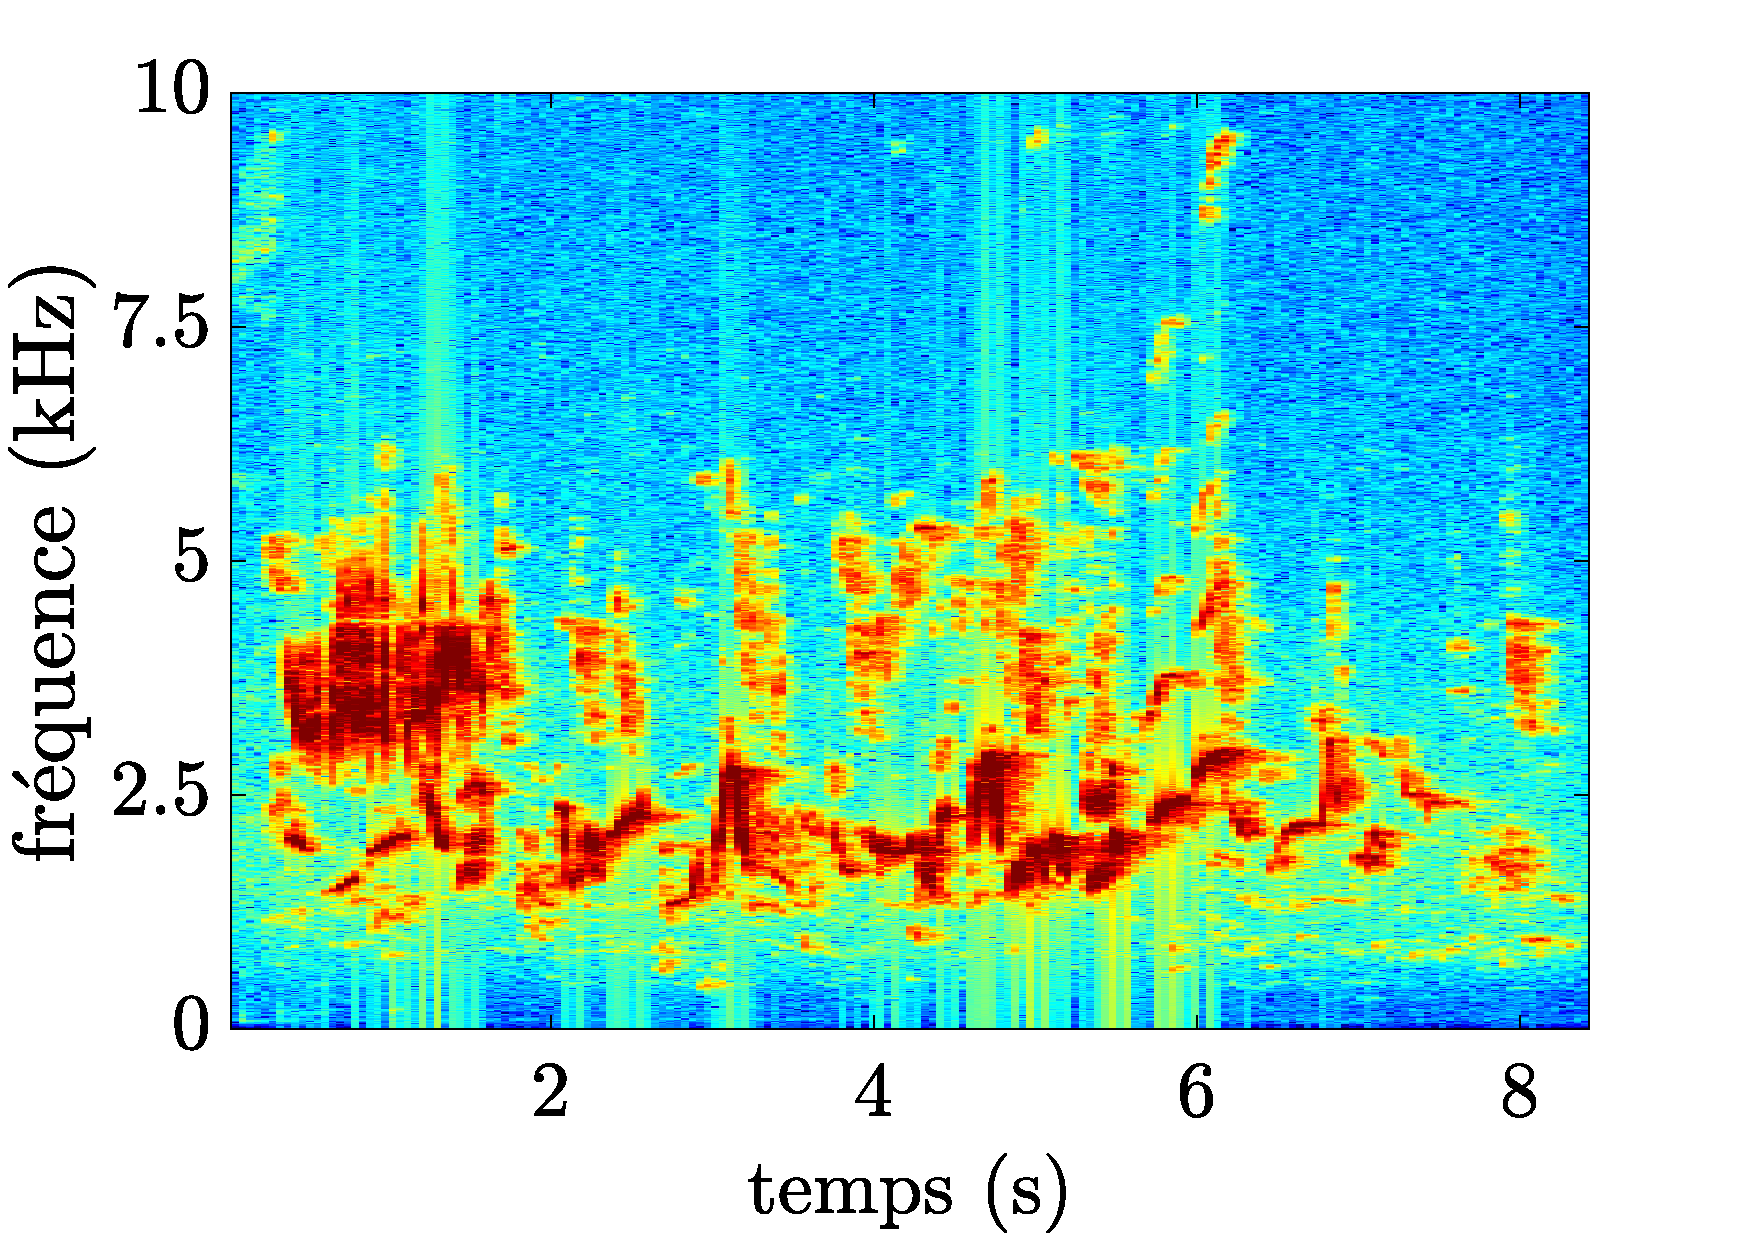
\includegraphics [width=0.4\linewidth]{./figures/autres/sourcesUrbainesBird.pdf}}
\subfigure[\label{fig:sourceUrb3}]{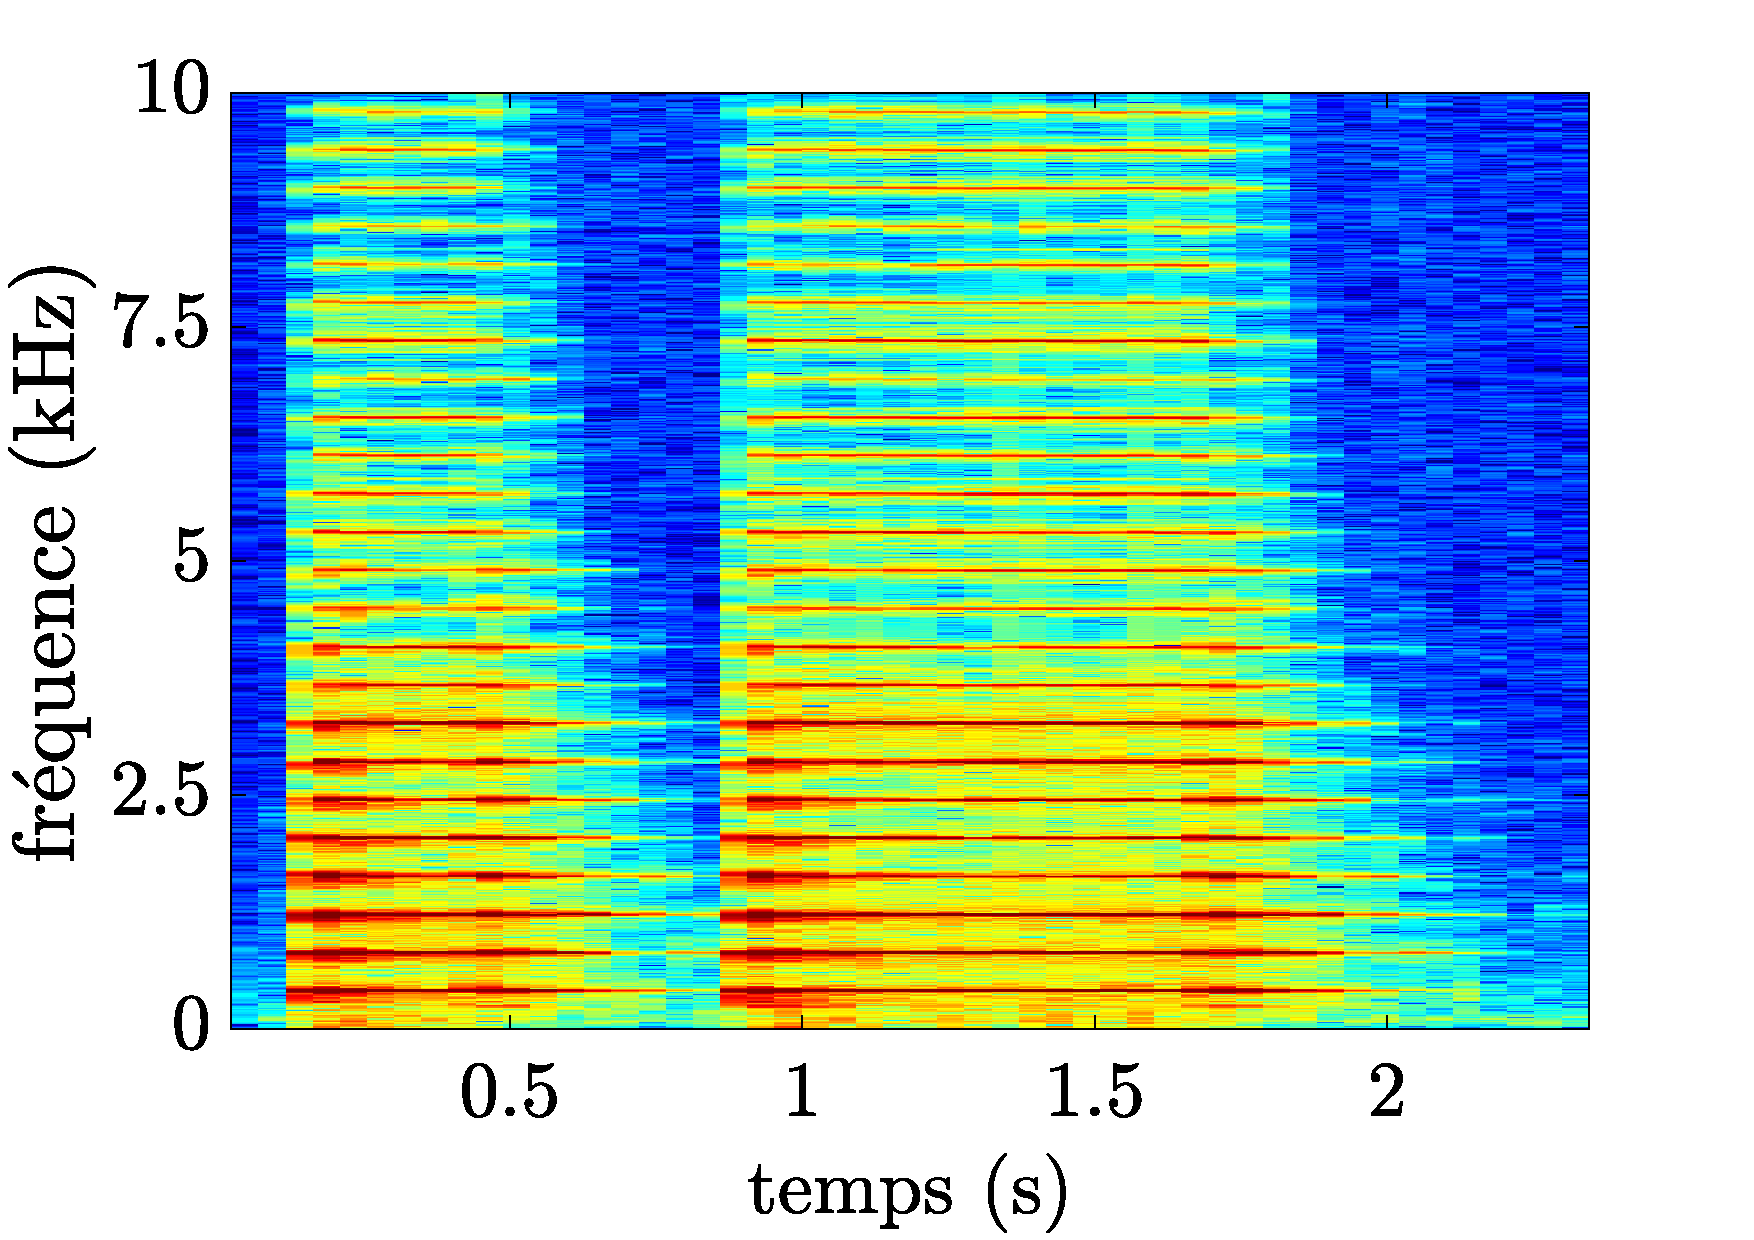
\includegraphics [width=0.4\linewidth]{./figures/autres/sourcesUrbainesCarHorn.pdf}}
\subfigure[\label{fig:sourceUrb4}]{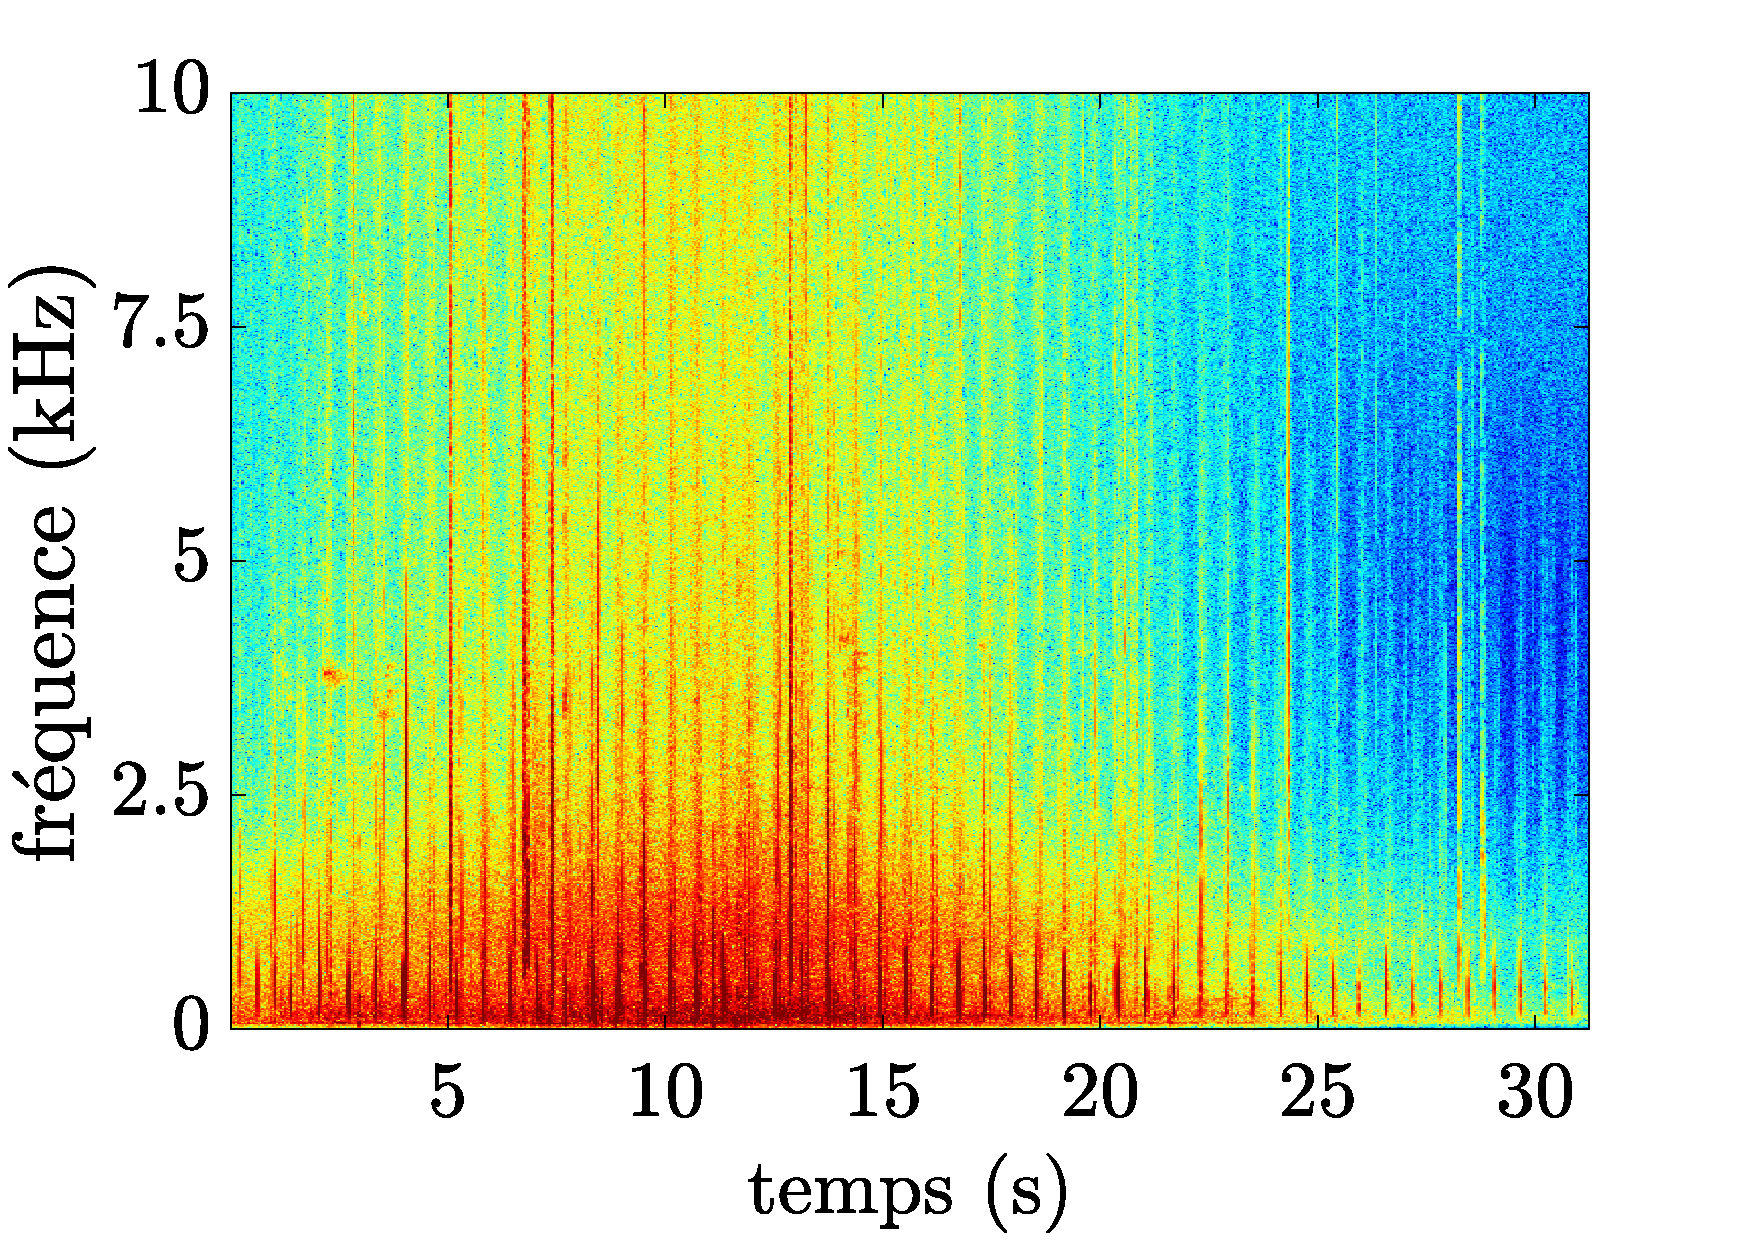
\includegraphics [width=0.4\linewidth]{./figures/autres/sourcesUrbainesFootStep.pdf}}
\caption{Spectrogrammes d'un passage d'une voiture \subref{fig:sourceUrb1}, d'un sifflement d'oiseaux \subref{fig:sourceUrb2}, d'un klaxon \subref{fig:sourceUrb3} et d'un bruit de pas \subref{fig:sourceUrb4}.}
\label{fig:sourceUrbain}
\end{figure}

En conséquence, les travaux de cette thèse cherchent à répondre à ces questions : 
\begin{itemize}
\item \textbf{Comment déterminer le niveau sonore des sources en villes ?}
\item \textbf{Quelles sont les méthodes disponibles pour réaliser cette tâches ? Quel est l'outil le plus adapté à cet environnement parmi ces méthodes ?}
\item \textbf{Quel protocole expérimental mettre en oeuvre pour tester et valider les performances de ces outils ?}
\end{itemize}


\section{Estimation du niveau sonore du trafic routier à partir de mesures} \label{part:cachier_charges}

\subsection{Objectifs}
Étant la source principale de bruit en ville ainsi que la plus gênante, le trafic routier sera la source d'intérêt qui sera principalement étudié. Le principe générale est résumé en Figure \ref{fig:estimateur0} : à partir d'un enregistrement audio (en format wav et de fréquence d'échantillonnage 44,1 kHz), un outil, appelé \textit{estimateur}, détermine le niveau sonore du trafic routier $\tilde{L}_{eq,trafic}$.

\begin{figure}[t]
\centering
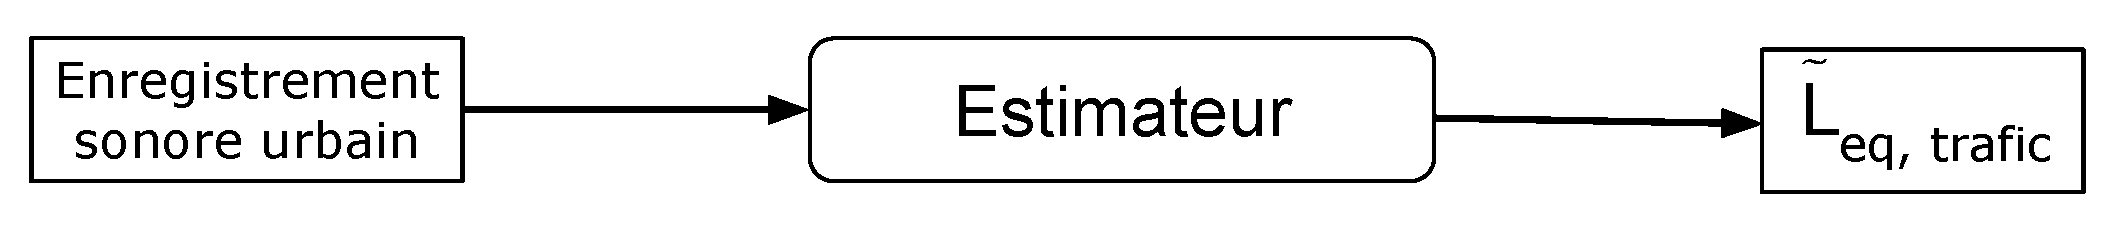
\includegraphics[width=0.7\linewidth]{./figures/NMF/bloc_diagram_estimateur0.pdf}
\caption{Diagramme bloc de l'approche proposée.}
\label{fig:estimateur0}
\end{figure}

L'objectif est donc de construire cet estimateur et un protocole expérimental adéquat afin d'obtenir la meilleure estimation possible du niveau sonore du trafic.

\subsection{Protocole expérimental}

Si plusieurs études se sont déjà intéressées au trafic routier au sein d'environnements sonores urbains (reconnaissance du bruit de véhicule \cite{defreville_automatic_2006}, estimation du débit véhicule \cite{torija2012using}, détection des accidents \cite{harlow2001automated}, estimation des trajectoires \cite{leiba2017large}), la détermination de son niveau sonore a pour l'instant été très peu étudiée. On peut citer récemment les travaux réalisé au sein du projet DYNAMAP \cite{socoro2017anomalous}. Leur approche consiste à entrainer une méthode de détection en vue d'estimer les évènements qui n'appartiennent pas à la classe de son \textit{trafic} afin de ne pas les considérer lors de l'estimation des niveaux sonores. Ici, l'approche choisie est différente : l'estimateur du niveau sonore du trafic routier s'appuie sur une méthode de séparation de sources afin d'extraire l'intégralité de la composante \textit{trafic} des enregistrements audio parmi les autres sources sonores présentes (voir Figure \ref{fig:separation_source}). De cette extraction, le niveau sonore trafic $\tilde{L}_{eq,trafic}$ est calculé.

\begin{figure}[t]
\centering
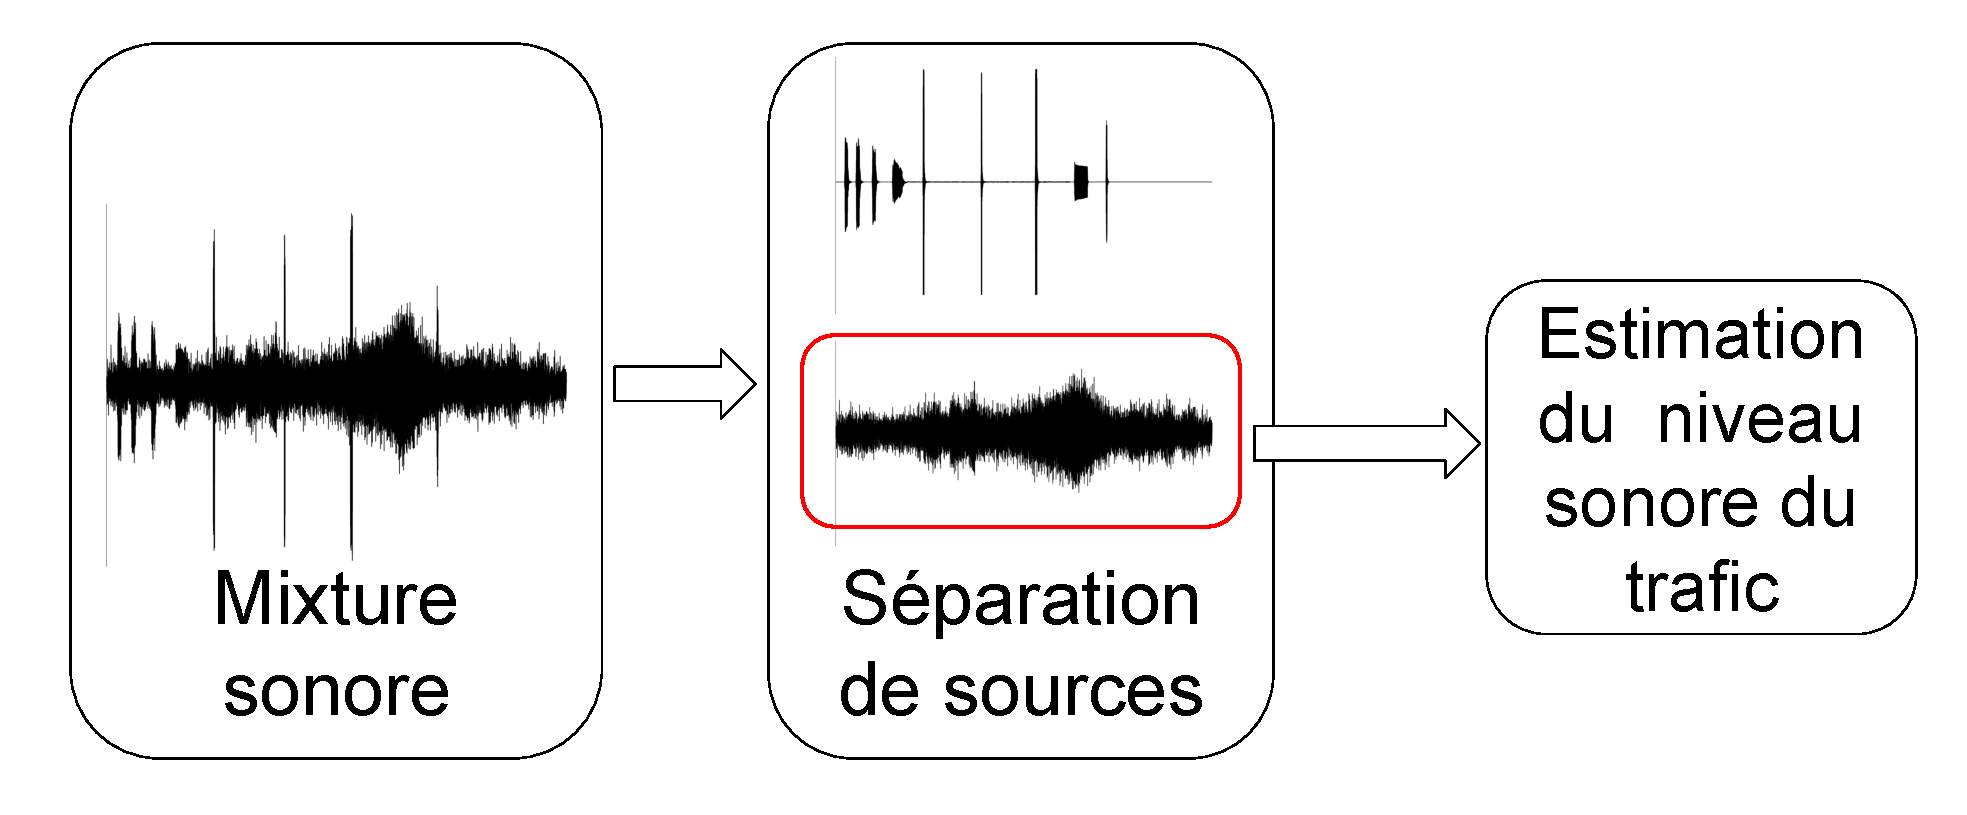
\includegraphics[width=0.7\linewidth]{./figures/NMF/bloc_diagram_source_separation.pdf}
\caption{Diagramme en bloc de l'approche par séparation de sources.}
\label{fig:separation_source}
\end{figure}

Une question reste toutefois à résoudre : comment, à partir d'enregistrements audio, être certain que l'estimateur donne une valeur correcte du niveau sonore du trafic ? Dans le cas où il n'y a que du trafic, l'estimation fournie par la méthode peut être facilement comparée mais quid des scènes sonores où le trafic n'est pas prépondérant et est recouvert par d'autres sources sonores ? La valeur exacte du trafic, $L_{eq,trafic}$, est l'inconnue qu'on cherche justement à déterminer. Sans cette valeur de référence, il est impossible de comparer la valeur déterminée et ainsi la validité et les performances de l'estimateur.
Le choix est donc fait d'utiliser des corpus de scènes sonores issus d'un processus de simulation où un contrôle total des classes sonores présentes, ainsi que de leur niveau sonore, est alors possible. La valeur exacte, $L_{eq,trafic}$, est alors obtenue. La figure \ref{fig:diagramBlocProtocol} résume le schéma global du procédé suivi.

\begin{figure}[t]
\centering
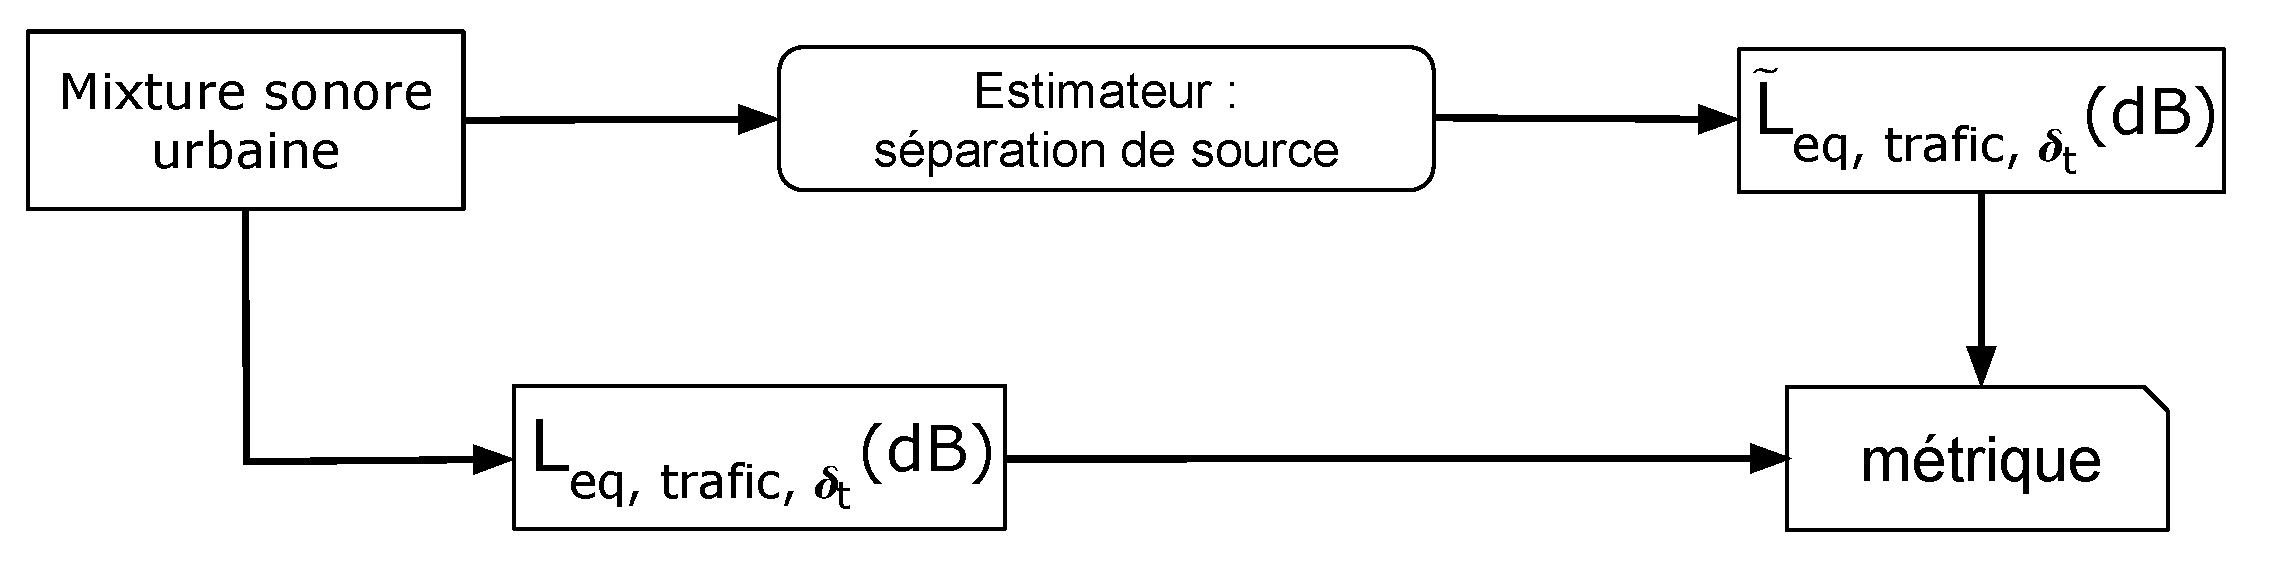
\includegraphics[width=0.7\linewidth]{./figures/NMF/Bloc_diagram_estimateur_FR.pdf}
\caption{Diagramme bloc du protocole expérimental.}
\label{fig:diagramBlocProtocol}
\end{figure}

Se pose alors la question du niveau sonore calculé par scène : choisit-on un niveau sonore à court-terme toutes les 125 ms ? toutes les secondes ? toutes les minutes ? pondéré $A$ ? Aux vues de l'utilisation de cet estimateur qui est faite (meilleur estimation de la contribution du trafic, amélioration de la cartographie des cartes de bruits en ville), le choix est fait de choisir une durée adaptée à cet outil et ainsi de calculer le niveau sonore du trafic chaque minute, $\L_{eq,trafic,60s}$. Enfin, on ne  considère aucune pondération afin de se focaliser sur une estimation physique du niveau \textit{trafic}.\\

Les niveaux sonores exactes et estimés, produits sur un ensemble de $M$ scènes testés, sont ensuite comparés à travers un calcul de métrique. Parmi les différentes métriques possibles (somme des carrés des résidus, la racine de l'erreur quadratique moyenne $RMSE$ \dots), l'erreur absolue moyenne, $MAE$ (pour \textit{Mean Absolute Error}) est retenue : 

\begin{equation}
MAE = \frac{\sum_{i = 1}^{M} \vert L_{eq, trafic, 60s}^i - \tilde{L}_{eq, trafic, 60s}^i \vert}{M}.
\end{equation}

Contrairement à l'erreur RMSE, qui revient à la racine carré de la moyenne du carré des différences entre les données observées et réelles, qui pénalise plus les valeurs qui dévie fortement, l'erreur $MAE$ présente l'intérêt de considérer un poids identique entre chaque différence et ainsi de gagner en interprétabilité.\\

Les questions à résoudre sont alors : 
\begin{itemize}
\item \textbf{Quelle méthode de séparation de sources choisir comme estimateur ?}
\item \textbf{Comment construire des corpus de scènes sonores urbaines pour tester l'approche proposée ?}
\end{itemize}

%
%%\bibliographystyle{unsrt}
%%\bibliography{../bibliographie}
%%
%%\end{document} 
%
%%\subsection{Incertitudes liées à la modélisation numérique}
%%
%%Les cartes de bruits étant simulées, des problèmes apparaissent également lié à la modélisation et à la discrétisation du milieu urbain. Afin de limité la durée des calculs de techniques d'optimisation sont utilisées comme la discrétisation du milieu mais aussi des sources de bruits. Par exemple, pour une route décrite comme une source linéique de bruit, celle est discrétisé en un ensemble de source ponctuel alignées. Le choix de la distance entre ces points est alors un compromis à faire entre temps de calcul et précision souhaitée. Toutefois la position de ces sources influe ensuite sur les phénomènes de réflexion et de diffraction. De plus, afin de réduire les temps de calculs, les niveaux sonores entre les points calculés sont déterminés au moyen d'un calcul d'interpolation (méthode de Krigeage) qui viennent donc rajouter en plus des incertitudes \cite{van_leeuwen_noise_2015}. 
%%
%%IMAGE d'INTERPOLATION ?
%%
%%Enfin toujours en raison de la limitation des moyens numériques, l'effet de l'architecture urbaine (balcon, fenêtre) ou du mobilier urbain n'est pas pris en compte dans la modélisation des villes car trop complexe à réaliser alors que ces éléments ont un impact qui n'est pas pris en compte. 
%%
%%\subsection{Représentation des données et estimation du nombre de citadins touché}
%%
%%Une fois les cartes produites, indépendamment des remarques faites précédemment, une des critiques quant aux cartes de bruits est la limitation d'informations qu'elle produisent : un niveau sonore $L_{DEN}$ et $L_N$ pour décrire le niveau sonore du trafic. Ces deux seules indicateurs permettent certes d'avoir un aperçu global d'une grandeur qui, pourtant, évolue constamment. En effet, aussi bien à l'échelle de l'année ou d'une journée, le trafic routier évolue sans cesse. Cette évolution peut se diviser en 4 parties : un pic de trafic situé entre 7h et 9h et entre 16h et 18h correspondant au moment où les citadins emprunte leur voiture pour se déplacer entre leur domicile et leur travail. Entre ces 2 périodes, la quantité de voiture est plus faible \cite{}. La prise en compte ces évolutions de débit de trafic dans les modèles afin de simuler des cartes heures par heures est toutefois compliqué à mettre en œuvre car elle nécessiterait de grande quantité de ressources informatiques et cette approche ne permettrait pas d'obtenir l'évolution annuelle.
%%Coupler les modèles de sources et de propagation à des modèles dynamiques de trafic est une voie pour créer des cartes de bruit de trafic dynamiques prédictives. 
%%
%% Dans \cite{modiuszeski}, Modiuszeski compare le niveau sonore simulée prédit par la carte de bruit avec les résultats de mesures réalisée toute l'année. Il constate alors aisément que l'évolution des niveaux sonores évolue autant à l'échelle de la journée que de l'année rendant les valeurs $L_{DEN}$ et $L_N$ extrêmement restrictives. Enfin, au fur et à mesure que la perception du citadin de l'environnement sonore est mieux connu, il a été montré que les indicateurs de niveaux sonores du trafic pondéré A n'est pas suffisant pour rendre compte de sa perception de l'environnement sonore. Selon, le cadre architecturale de la ville, le statu social du citadin et les sources sonores présentes, pour un niveau sonore trafic similaire, l'agrément de l'ambiance sonore par le citatdin eut ne pas être la même. En conséquence, à partir des études sur le \textit{soundscape} \cite{schafer_soundscape_1993}, il peut être envisagé de réaliser des cartes de bruits, non plus liées à une seule source de bruit, mais à la perception du citadin de l'environnement sonore (\og agréable \fg{}, \og très désagréable \fg{}, \dots). Ces cartes ne se feraient plus alors à partir d'une source de bruit mais sur l'ensemble des sources sonores présentes dans les zones et permettraient, au citadin, de savoir si tel quartier a un environnement sonore agréable ou non.\\
%%
%%Des indicateurs de niveaux sonore, le nombre de citadins exposés au bruit peut être déterminé. Là encore, la méthode pour estimer ce chiffre est discutable. King et Murphy résument cela dans un paragraphe dans \cite{king_implementation_2011}. L'hypothèse faite est que les individus vivent et dorment toute l'année au niveau de la façade la plus exposée, ce qui n'est pas forcément représentatif de la réalité. Cette hypothèse conduit notamment à une surestimation du nombre de personnes touché par des niveaux sonores. \\
%%
%%La réalisation de ces cartes visant à diminuer l'exposition des citadins au forts niveaux sonores, les incertitudes provoquées par les différents étapes peuvent entrainer la mise en chantier d'un plan d'action mal adapté à la situation réelle. Mais l'amélioration des cartes, telles qu'elles sont faites actuellement, semble toutefois limité : l'augmentation de la résolution des permettrait bien de corriger certaines erreurs dû aux interpolations mais viendrait à augmenter considérablement les cout de calculs. De plus, ce choix rendrait impossible de mettre à jours les cartes régulièrement pour prendre en compte les fluctuations du trafic à l'échelle de l'année ou même encore durant la journée. En conséquence, à l'heure où les villes s'équipent en réseaux de capteurs (météorologique, qualité de l'air) en vue de devenir des \og villes intelligentes \fg{} (\textit{smart cities} en anglais), il devient possible d'ajouter des capteurs acoustiques afin de s'en servir pour décrire l'environnement sonore urbain. \\
%


%\subsection{Cartographie des ESU}
%
%D'autres études se sont intéressées aux ESU de manière plus générale afin de classifier les environnements sonores par ambiance à partir de différents indicateurs physiques comme dans \cite{can_describing_2015} où le niveau sonore équivalent pondéré $A$, son écart type et le centre de gravité spectrale entre les bandes de 50 Hz et 10 kHz sont considérés pour discriminer les ambiances sonores. Dans \cite{salamon2015unsupervised}, Salamon et Bello utilisent un algorithme de k-moyenne sphérique en tant que classifieur. 
%La cartographie de l'ESU selon des ambiances sonores défini (\textit{parc}, \textit{rue piétonne}, \textit{boulevard} \dots) est alors possible pour offrir une autre représentation de la ville lié non pas à une source sonore spécifique mais à la somme des différentes sources présentes sans distinction entre elles.  

%Une autre piste à l'étude est la description des ESU à travers la perception du citadin \cite{brocolini_measurements_2013}.
%Cette approche est résumée sous la notion de paysage sonore (ou \textit{soundscape} en anglais). Proposée par R. Murray Schafer \cite{schafer1977tuning}, cette notion considère que la perception de l'ESU par le citadin est liée à sa construction sociale (âge, expérience, milieu social\dots), là où l'ESU est le résultat de phénomènes physiques (source sonores, diffusion du son, réverbération\dots). 

%En conséquence, plusieurs études se sont intéressées à l'évaluation de l'ESU aux travers de descripteurs acoustique sémantiques (Evaluation de la scène, clarté, occupation spatiale, évolution temporelle)  \cite{raimbault2003ambient,hall2013exploratory}, afin de définir les éléments (sources sonores, environnements) qui sont les plus gênants ou bien les plus appréciés. 
%D'autre études, en vue de prédire le paysage sonore, lient la perception de l'ESU à des indicateurs physiques (niveau sonore pondéré, niveau sonore fractile $L_x$\dots). Ces modèles prédictifs peuvent être établi à partir d'écoutes réalisées en laboratoire comme dans \cite{torija2013application} où le paysage sonore est décrit à partir de 14 indicateurs dont le facteur crête (rapport du niveau sonore maximum sur le niveau sonore équivalent à 15 minutes), le niveau sonore pondéré $A$ des signaux contenant une réponse impulsionnelle ou les niveaux sonores des bandes de tiers d'octave de 125 Hz et 16 kHz.
%Il est également possible de réaliser des marches sonores en ville (ou \textit{soundwalk} en anglais). Cette approche consiste à faire évaluer l'ESU à des auditeurs le long d'un parcours effectué en ville. Intiallement proposée par \cite{southworth1967sonic}, la réalisation de \textit{soundwalk} a ensuite été popularisée par R. M. Schafer dans le concept du \textit{soundscape} où sa pratique est centrale dans l'étude de l'ESU \cite{schafer1969new, schafer1977tuning}. Ces marches présentent l'avantage de permettre une représentation du monde plus réaliste que des écoutes en laboratoire et ainsi une meilleure validité écologique. Mais, les \textit{soundwalks} restent tributaires des sources sonores présentes dont le niveau sonore et la présence ne sont pas controlables. Ces études sont donc plus difficilement généralisables que celles réalisées en laboratoire. 

%Dans \cite{hong2014soundscape}, des cartes du paysage sonore urbain sont réalisées, à l'aide d'un logiciel SIG, à partir de l'évaluation perceptive de la présence du trafic, des sons technologiques, des sons humains et des sons naturels ainsi que de l'évaluation du paysage sonore et de l'environnement urbain. Ces évaluations sont complétées par un seul indicateur physique, le niveau sonore équivalent pondéré $A$, $L_{A,eq}$. Cette étude révèle que le bruit de trafic perçu est corrélé au $L_{A,eq}$ alors que les sons naturels (sifflement d'oiseaux, bruit de fontaine) ne le sont pas (corrélation négative). Dans \cite{aumond2017modeling}, c'est la notion d'agrément sonore qui est défini (ESU plaisant ou déplaisant) à partir de deux modèles : l'un perceptif et l'autre physique. Le modèle perceptif est établit à partir du niveau sonores globale et du temps de présence de plusieurs source sonore spécifiques : trafic, voix, et oiseaux. Le modèle physique est basé sur des indicateurs physiques tels que le niveau sonore fractile $L_{50}$ dans la bande de tiers d'octave de 1 kHz ainsi que la variation normalisée en temps et en fréquence des bandes de 500 Hz et de 4 kHz. Ces indicateurs permettent de traduire la présence des sources sonores du modèle perceptif. 

%De ces différents modèles, réaliser des cartes de l'ESU perçu à partir des mesures issus des réseaux de capteurs serait alors envisageable et permettraient d'apporter une autre représentation de l'environnement sonore de la ville basée sur la perception du citadin et non sur les niveaux sonores physiques prédits des sources sonores les plus gênantes.

%\documentclass[twoside,openright,a4paper,11pt]{book}
%
%
\usepackage[utf8]{inputenc}
\usepackage[francais]{babel}
\usepackage[T1]{fontenc}

\addto\captionsfrench{\def\tablename{\textsc{Tableau}}}% pour avoir TABLEAU et pas TABLE dans les légendes des tableaux

%%%%%%% MISE EN PAGES %%%%%%
\usepackage{geometry}
\geometry{outer=2cm,inner=3cm,top=3cm}

\setcounter{tocdepth}{3}     % Dans la table des matieres
\setcounter{secnumdepth}{3}  % Avec un numero.
\usepackage{setspace}

\usepackage{fancyhdr}	% marge en haut et en bas
\pagestyle{fancy}

\fancyhead{}	% vide l'entête
\fancyfoot{} % vide le pied~de~page

\fancyhead[RO]{\leftmark}
\fancyhead[LE]{\rightmark}
\fancyfoot[C]{\thepage}	% numéro de page en bas au centre

\renewcommand{\headrulewidth}{0.4pt} % épaisseur du trait en haut
\renewcommand{\footrulewidth}{0.4pt} % épaisseur du trait en bas

\fancypagestyle{mypagestyle}{%
    \fancyhead{}	
    \fancyfoot{} 
    \fancyfoot[C]{\thepage}
    \renewcommand{\headrulewidth}{0.4pt} 
	\renewcommand{\footrulewidth}{0.4pt} 
}

\fancypagestyle{couvertureAbstract}{%
    \fancyhead{}	
    \fancyfoot{} 
    \fancyfoot[C]{}
	\renewcommand{\headrulewidth}{0pt} 
	\renewcommand{\footrulewidth}{0pt} 
}
%
\usepackage{layout}
\usepackage{tocbibind} % include tableofcontent in itself

%%%%%% PAGE DE GARDE %%%%%%

\geometry{outer=2cm,inner=3cm,top=3cm}
\usepackage[scaled]{helvet} % font used on cover (Helvetica)
\usepackage{eso-pic} % to set background picture
\usepackage{multicol} % for back cover (abstracts)
\usepackage{graphicx} % to include logos
\usepackage{tikz} % to compose background picture

% Colors (extracted from SPI's template)
\definecolor{boxcolor1}{rgb}{0.91373,0.92941,0.87451}
\definecolor{boxcolor2}{rgb}{0.94902,0.93333,0.91373}
\definecolor{boxcolor3}{rgb}{0.76078,0.87843,0.17647}
\definecolor{headercolor}{rgb}{0.94118,0.30980,0.17255}
\definecolor{namecolor}{rgb}{1.0,0.4,0.0}
\definecolor{titlecolor}{rgb}{0.19216,0.51765,0.60784}
% Also used: gray, teal (predefined by xcolor package, usually loaded by document class)

% Cover environment, to keep changes local
\newenvironment{cover}{%
  \fontfamily{phv}\selectfont % Select Helvetica font
  \pagestyle{empty} % No page number
}{
  \addtocounter{page}{-1}
  \cleardoublepage
}

% Macro for background common to front and back
\newcommand{\tikzBG}{%
  \path (0,0) rectangle (1,1);
  %TODO: You should adjust the bottom height of the following rectangle to fit your abstract's length
  \path [fill=boxcolor1] (.0571,.11) rectangle (.481,.963); 
  \path [fill=boxcolor2] (.4333,.697) rectangle (.9048,.7475);
  \path [fill=boxcolor2] (.4333,.7811) rectangle (.9048,.8316);
  \path [fill=boxcolor2] (.4333,.8687) rectangle (.9048,.9192);
  \path [fill=boxcolor3] (.0571,.7879) rectangle (.5762,.8316);
  \node[inner sep=0pt] at (0.2285,0.8788) [above left] {%
    
\includegraphics[height=.0707\paperheight,keepaspectratio]{./figures/logo/logo_unb.png}};
  \node[inner sep=0pt] at (0.6667,0.8788) [above right] {%
    
\includegraphics[height=.0808\paperheight,keepaspectratio]{./figures/logo/logo_ecn_color.png}};
  \node at (.0571,.8316) [above right,color=headercolor] {%
    \fontsize{29}{35}\selectfont\bfseries Th\`ese de Doctorat};
}

% Macro for repeated information (to avoid insconsistency)
%TODO: fill in with no formatting but desired case
\newcommand{\firstName}{Jean-Rémy}
\newcommand{\surname}{Gloaguen}
\newcommand{\thesisTitle}{Estimation du niveau sonore de sources d'intérêts au sein de mixtures sonores urbaines : application au trafic routier}

%%%%%%% SYMBOLES %%%%%
\usepackage{tipa}	% pour avoir l'accent concave
\usepackage{lmodern}	% pour les guillemets
\usepackage{gensymb}	% pour les degrés
\usepackage{enumitem}	% pour changer le symbole de l'item (\begin{itemize}[label=$\bullet$])

%%%%%%% EQUATION %%%%%%
\usepackage{amssymb}
\usepackage{amsmath}
\usepackage{fancybox}
\usepackage{xfrac}	% fraction de type "1/4"
\usepackage{cases}	% système équation
\usepackage[overload]{empheq}
\usepackage{bm}		% pour mettre en gras .
\usepackage{units} 	% x/y barre latérale pour les fractions
%
%%%%%%% FIGURE %%%%%%
\usepackage{subfigure}	% utiliser subfigure
\usepackage{float}	% utiliser H dans les figures
%
%%%%%% TABLEAUX %%%%%%
\usepackage{array,multirow,makecell}
%\addto\captionsfrench{\def\tablename{\textsc{Tableau}}}% pour avoir TABLEAU et pas TABLE dans les légendes des tableaux
\usepackage{colortbl} % pour avoir des lignes colorées dans les tableau
%\usepackage{slashbox} % pour les \backslashbox
%\usepackage{subcaption}
\usepackage{hhline}	% pour les lignes horizontales 
\usepackage{tabularx} % permet itemize dans les cellules
\usepackage{booktabs}
\usepackage{longtable}	% pour les tableaux longs

\newcolumntype{L}[1]{>{\raggedright\let\newline\\\arraybackslash\hspace{0pt}}m{#1}}
\newcolumntype{C}[1]{>{\centering\let\newline\\\arraybackslash\hspace{0pt}}m{#1}}
\newcolumntype{R}[1]{>{\raggedleft\let\newline\\\arraybackslash\hspace{0pt}}m{#1}}

%%%%% ALGORITHME %%%%%
\usepackage{algorithm}
\usepackage{algorithmic}

%%%%% BIBLIO %%%%%
\usepackage[fixlanguage]{babelbib}
\selectbiblanguage{french}
\usepackage{breakcites}	% pour couper les références en bout de ligne

%%%%% APPENDICES %%%%%%%
\usepackage[toc,page]{appendix}

%%%%%%%%%%%%%%%%%%%%%
\usepackage{url}	% gérer les adresses www.
\linespread{1.2}	% interligne

\cleardoublepage
%
%\begin{document}
%\newpage

\chapter{Identification, détection et séparation des sources sonores}

La détection, l'identification ou la séparation d'une source sonore dans le cadre de sons environnementaux (qui ne contiennent ni de la musique, ni de la parole) est un sujet complexe car cette catégorie inclut des sons extrêmement variés aussi bien en temps qu'en fréquence. De prime abord, ces méthodes de traitement du signal ont été appliquées pour des signaux contenant de la voix et de la musique car leur structure est beaucoup mieux prédictive et connue. L'application de ces méthodes se fait en deux phases : une phase d'apprentissage où les algorithmes sont testé sur des bases de données connues et qui permet de déterminer le comportement de l'outil puis une phase de test où ce modèle est appliqué à une base de données inconnues. De nombreuses études se sont intéressés à savoir détecter les différents évènements sonores présent dans un scène. Les outils utilisés seront présenté dans la partie \ref{sec:ident_detec}. Enfin, souhaitant isoler le trafic routier des autres sources sonores, ce sont les méthodes de séparation de sources qui seront revues dans la partie

\section{Méthodes de détection et d'identification}
\label{sec:ident_detec}

Lorsqu'on parle de classification, il s'agit de savoir automatiquement savoir si un extrait audio appartient à une catégorie ou à une autre. Il peut s'agir de classer un morceau de musique selon son style \cite{tzanetakis_musical_2002}, de classer un enregistrement sonore selon son environnement sonore \cite{chu_where_2006}. Lorsqu'on parle de détection, on parle de la détermination du temps de présence des différents évènements sonores dans un scène sonore mais également à déterminer la source sonore correspondante. Cette tâche trouve notamment son intérêt lors des phases d'annotation de scènes sonore où un auditeur estime à la main le temps d'apparition et de fin des différents évènements, tâche qui peut être très fastidieuse et complexe \cite{mesaros_sound_2015} \cite{cakir_polyphonic_2015}. \\

Afin de comparer les performances des algorithmes, plusieurs bases de données on été conçu, lors de challenges, afin d'être utiliser pour les tester. Dans le cas de la parole, la base de données CHiME \cite{christensen_chime_2010} est la plus souvent utilisée \cite{barker_pascal_2013} \cite{araki_2011_2012}. Pour la musique, des bases de données, comme RWC \cite{goto_rwc_2003} et CAL500 \cite{wang_towards_2014}, existent et servent pour des tâches comme la classification par genre musicaux ou à la définition des structures musicales. Certaines base de données sont même destinées à une classe d'instrument particulière (comme les instruments percussifs pour la base de données , ENST-drums \cite{gillet_enst-drums:_2006}). \\

Si ces base de données et challenge on été destiné à la parole et à la musique, c'est à partir de 2013 qu'est crée le challenge \textit{Detection $\&$ Classification of Acoustics Scene Event} (DCASE) \cite{giannoulis_detection_2013} qui s'adresse aux sons environnementaux. La lecture des articles résumant les techniques ainsi que les résultats permet de connaitre les méthodes qui sont plébiscités. \\


De nombreux modèles de classificateur ou de détecteur adapté à des sons urbains utilisent les même outils que pour les sons de paroles ou musicaux. Cette partie présente les approches et les différents outils les plus couramment utilisés. Le modèle de classification est réalisée en deux étapes. Les signaux audio sont d'abord décrits par des descripteurs qui vont donner une représentation réduite des classes de sons visées. Un classificateur est ensuite utilisé permettant ainsi de distinguer les différentes classes de sons présentes dans le signal audio. La partie~\ref{part:descripteur} et \ref{part:classificateur} exposent respectivement les différents descripteurs et classificateurs couramment utilisées.

\subsection{Descripteurs}\label{part:descripteur}
Un large nombre de descripteurs ont déjà été utilisé dans la littérature \cite{} \cite{} \cite{}. Ces descripteurs peuvent décrire un signal à la foi dans le domaine temporel que fréquentiel. Ils permettent de réduire la dimension du signal audio à quelques valeurs simplifiant la classification. Pour être optimal, le choix de ces descripteurs doit permettre une description unique des classes de sons. Dans \cite{}, Peeters résume un grand nombre de paramètres couramment utilisé qu'il regroupe dans le projet CUIDADO. Il classe les paramètres en 5 familles : les paramètres temporels, énergétiques, spectraux, harmoniques et perceptifs.

\begin{itemize}
\item \textbf{paramètres temporels} : il résume aussi bien les paramètres qui décrive un signal sur des parties entière du signal (par exemple l'attaque, la tenue et l'extinction du isgnal) que de manière instantanée avec la fonction d'auto-corrélation ou le \textit{Zero-Crossing Rate} qui énumère le nombre de fois qu'un signal traverse l'axe des zéro. Un faible ZCR traduit un signal harmonique alors qu'un grand ZCR signifie le son est composé de bruit. 

\item \textbf{paramètres énergétiques} : Il résume les indicateurs énergétique aussi bien du signal entier que de partie plus restreinte ou bien encore celles des composantes harmoniques ou du bruits.

\item \textbf{paramètres spectrales} : C'est une classe de descripteurs large. Elle contient des descripteurs simples comme le centre de gravité spectrale ou qui calcule l'évolution temporel du spectre (ou flux spectral) comme des descripteurs plus complexe comme les LPCC (Linear Predictive Cepstral Coefficient) et les MFCC (Mel Frequency Cepstral Coefficient). Les MFCC sont couramment utilisés dans les tâches de classification ou de détection. Ils consistent à exprimer la transformée de Fourier d'un signal par des bandes Mel et à réaliser à transformée en cosinus discret du logarithme du signal obtenu (figure \ref{fig:schema_mfcc}).

\begin{figure}[h]
\centering

\includegraphics[width = 0.7\textwidth]{./figures/autres/schema_MFCC.pdf}
\caption{Schéma de la conception des MFCC}
\label{fig:schema_mfcc}
\end{figure}

L'échelle Mel est une échelle de hauteur de sons issus de la psycho-acoustique. Son échelle est construite afin qu'un doublement de mel corresponde à un doublement de la fréquence perçu. Par exemple pour un son pur à 1000 Hz (correspondant à 1000 mel), le son perçu deux fois plus aigu sera un son à environ 3428 Hz et non à 2000 Hz. L'échelle des Mel est alors définit par la relation \ref{eq:melScale} permettant ainsi de conserver le rapport 2 entre les deux sons (le signal à 3428 Hz est alors à 2000 mel),

\begin{equation}\label{eq:melScale}
mel = 1127 \ln\left(1+\frac{f}{700}\right).
\end{equation}


\item \textbf{paramètres harmoniques} : Cette catégorie regroupe des descripteurs comme la détermination de la fréquence fondamental, de  l'inharmonicité ou bien du tristimulus du signal.

\item \textbf{paramètres perceptifs} : Cette dernière classe regroupe les indicateurs psycho-acoustique comme l'acuité ou la sonie du signal.\\
\end{itemize}

Dans son article, Peeters \cite{Peeters} résume un ensemble de descripteurs couramment utilisés dans le domaine de la reconnaissance de parole \cite{Kim} ou le domaine de la musique \cite{Fu} qui sont ceux qui sont également utilisés pour des ambiances sonores environnementales \cite{Cowling}, \cite{Haddad}, \cite{Defreville}. 


%
%En raison de l'utilisation de l'échelle Mel, les MFCC sont le plus souvent utilisés dans le cas de la détection de signaux de paroles \cite{Wu}.

%\subsection{Analyse en Composante Principale}\label{part:ACP}
%
%L'utilisation de plusieurs descripteurs génèrent un ensemble de données décrivant chaque signal spécifiquement. 
%
%\begin{equation}
%\mathbf{X} = 
%\begin{pmatrix}
%x_{11}& x_{12} & \dots & x_{1p} \\
%x_{21}& x_{22} & \dots & x_{2p} \\
%\vdots & \vdots & \ddots & \vdots \\
%x_{N1}& x_{N2} & \dots & x_{Np}
%\end{pmatrix}
%\end{equation}
%
%où $N$ est le nombre de signaux traités et $p$ le nombre de variable utilisé pour les décrire. Néanmoins, leur représentation graphique en un nuage de point qui permettrait de visualiser la corrélation entre les signaux n'est pas facile au delà de $p = 3$ car la dimension de problème n'est alors plus représentable. De plus, certains paramètres sont parfois redondant et ajoute une dimension aux problème rendant la représentations des corrélations entre elles plus difficile. \\
%
%L'Analyse en Composante Principale (ACP) se propose alors de réduire les dimensions du problème en passant d'un espace à $p$ dimensions à un sous-espace réduit $k$ (le plus généralement $k = 2$ ou $k=3$). Ces nouvelles variables $k$ sont construites à partir de combinaisons linéaire des $p$ variables initiales et celle qui présentent les plus fortes variances. Elles sont appelées \og composante principale \fg{} et forment de nouveaux axes de représentations appelé \og axes principaux \fg{}. Ce choix permet de conserver le plus d'information possible. Pour cela le sous-espace est construit afin que sa distance avec les données de $\textbf{X}$ soit minimale et que la projection du nuage de points est une dispersion (ou inertie) maximale.
%
%L'extraction de paramètres des signaux permet alors d'apporter de nouvelles informations qui vont permettre ainsi de séparer les signaux en fonction des classes de son présentes. Leur choix doit permettre de rendre chaque description des classe unique afin que la classification soit réussie.

\subsection{Classificateurs}\label{part:classificateur}

L'étape de classification vise à reconnaitre les différentes classes de sons présentes à l'aide des descripteurs offrant ainsi une référence qui permettra la reconnaissance des sources lors de la phase de test. Les méthodes de classification peuvent être considéré par deux approches : discriminative ou générative.\\

La première approche modélisent directement la règle de classification. Les plus populaires sont les \og $k$-plus-proches voisins \fg{} ($k$-NN pour \textit{k-Nearest-Neighbours} en anglais) ou les Vecteurs à Support de Machine (SVM pour \textit{Support Machine Vectors} en anglais). \\

La méthode $\mathbf{k-}$\textbf{NN} consiste à calculer les distances entre un échantillon testé $x$ et les données issus de l'apprentissage. La classe ayant alors les $k$ distances les plus faibles est donc celle de l'échantillon $x$.\\

La méthode \textbf{SVM}, quant à elle, consiste à déterminer un séparateur linéaire entre deux ensembles de telle façon que la distance normal des plus proches échantillons des classes à cette courbe soit maximisée. Cette courbe est appelé \textit{hyperplan} et les échantillons qui maximisent la distance sont les \textit{vecteurs supports}. Dans le cas où le problème ne possède pas d'hyperplan linéaire, l'espace de représentation des données est modifié, pouvant jusqu'à être défini dans un espace à dimension infini, afin d'en obtenir un.\\

Les méthodes génératrices visent à modifier la distribution des données $x$ pour ensuite réaliser la classification. Les plus utilisés sont les Modèles de Mixtures Gaussiens (abrégé GMM pour \textit{Gaussian Mixture Models} en anglais) et le Modèle de Markov Caché (HMM pour \textit{Hidden Markov Model}).\\

Un modèle de mélanges gaussiens modélise une distribution de données comme une somme de gaussiennes pondérées (équation \ref{eq:GMM}). 

\begin{equation}\label{eq:GMM}
g(x,\bm{\mu},\bm{\sigma}) = \sum_{n = 1}^N \pi_n f(x,\bm{\mu}, \bm{\sigma})
\end{equation}

avec pour distribution gaussienne

\begin{equation}
f(x,\mu, \sigma) = \frac{1}{\sigma \sqrt{2\pi}}e^{\frac{(x-\mu)^2}{2\sigma^2}}
\end{equation}

%\begin{figure}[hbtp]
%\centering
%\includegraphics[scale=0.35]{../../../../Pictures/GMM.pdf}
%\caption{GMM (n trait plein) composé de deux distributions gaussiennes ($\bm{\pi} = \left[ 0.35,  0.75 \right]$, $\bm{\mu} = \left[9,  15.8 \right]$, $\bm{\sigma} = \left[ 3.2,  4.3 \right]$) pour $x \in \left[0~25 \right]$ }
%\end{figure}


C'est par l'algorithme de \textit{Esperance-Maximisation} \cite{Dempster} que les paramètres optimaux (moyenne $\bm{\mu}$, variance $\bm{\sigma}$, amplitude $\bm{\pi}$) sont trouvés. Le principe consiste à augmenter la probabilité entre le modèle et les données de manière itérative en effectuant deux phases de calculs distinctes :
\begin{itemize}
\item \og Espérance \fg{}, on estime des données inconnues, sachant les données observées ($x$) et la valeur des paramètres déterminée à l'itération précédente (moyenne et écart type dans le cas de distribution gaussienne). 
\item \og Maximisation \fg, on met à jours les paramètres en maximisant la vraisemblance de l'estimation des données et du modèle gaussien.\\
\end{itemize}

Cette étape de maximisation fait intervenir la règle d'inversion de Bayes (\ref{eq:Bayes}).

\begin{equation}\label{eq:Bayes}
P(y \in g_n \vert y) = \frac{P(y \vert y \in g_n)P(y \in g_n)}{P(y)}
\end{equation}

avec 
\begin{itemize}
\item $P(y \vert y \in g_n)$, la densité de probabilité de la classe $g_n$, 
\item $P(y \in g_n)$, la densité de probabilité de $y$, 
\item $P(y)$, la densité de probabilité de $y$ ($P(y) = 1$).\\
\end{itemize}

Lors de la phase de test, la classe $g_n$ dans laquelle l'élément testé $y$ a le plus de chance d'appartenir est déterminé en maximisant la probabilité à postériori $P(y\in g_n\vert y)$ (\ref{eq:maxArg}).

\begin{equation}\label{eq:maxArg}
f(y,\mu, \sigma) = \text{arg max } P(y\in g_n\vert y)
\end{equation}

Dans le cadre d'un GMM, (\ref{eq:Bayes}) devient 
\begin{equation}
P(y \in g_n) = \frac{\pi_n f(y,\mu,\sigma)}{\sum_{l = 1}^N \pi_l f(y,\mu, \sigma)}
\end{equation}

Une autre technique de classification couramment utilisé est le Modèle de Markov Caché \cite{Rabiner}. Le principe générale est de déterminer la succession la plus probable d'évènement à partir d'observations faites.\\
Cette méthode se base sur les chaines de Markov qui décrit l'état d'un processus stochastique à l'instant $t$ en fonction seulement de son état à l'instant $t-1$ avec la probabilité de passer d'un état $i$ à un état $j$ qui ne varie pas avec le temps.\\

Dans le cadre d'un modèle de Markov caché, l'état du système n'est pas disponible mais seulement des observations correspondant à l'état du processus. Le modèle dépend alors de 5 paramètres : 

\begin{itemize}
\item $S$, l'ensemble des états possibles,
\item $A$, l'ensemble des observations émis par les états,
\item $\Pi$, la loi de probabilité à l'état initial,
\item $T$, a matrice des probabilités de transitions d'un état à un autre.
\item $E$, la matrice de probabilité des observations pour chaque état.\\
\end{itemize}

C'est durant la phase d'apprentissage que l'ensemble de ces paramètres du modèle caché sont déterminé par la maximisation de vraisemblance (algorithme d'\textit{Espérance-Maximisation}). Chaque classe de son est alors caractérisé par un ensemble de paramètre. La phase de test cherche ensuite à maximiser la \textit{log}-vraisemblance (Maximum a Posteriori) entre les paramètres de l'échantillon testé et ceux issus de l'apprentissage.

Si ces techniques permettent d'identifier une source sonore, ce ne sont pas des outils adapté pour des mixtures sonores urbaines composée d'une multitude de sources très variés : trafic d'une voiture, d'un avion, bruit de pas, klaxon, oiseaux, musique... Ces sons ont des variations temporelles et fréquentielles très différentes. Pour cela, les techniques de séparations de sources semblent plus adaptés à ces ambiances sonores.

\subsection{Applications}

Ces méthodes de classification et de reconnaissance sont utilisée dans de nombreux domaines économique \cite{Hu}, médicale (\cite{Yu}, \cite{Gorriz}) ou de l'imagerie \cite{}.


Dans le cadre de signaux audiophoniques, les

Dans le cadre de la musique, ces techniques visent notamment à classer les musiques par genre, artistes ou époques (\cite{Tzanetakis}, \cite{Panagakis}, \cite{Berenzweig},\cite{Ellis}, \cite{Heitolla}). Ces outils trouvent leur intérêt dans l'utilisation et l'écoute de contenu musicaux sur internet (site de streaming par exemple) de plus en plus massive qui nécessite d'avoir des outils automatique de description des enregistrements audio afin de les classer mais aussi afin de suggérer à l'auditeur des contenus similaire qu'il pourrait aimer.  Les outils de séparation sont, quant à eux, notamment utile dans la restauration de vieux enregistrements.

Cowling, Haddad, Defréville...
Problème du recouvrement des sources sonores dans un milieu urbain

Delgado \& al. \cite{Delgado} se sont eux intéressé à ajouter un étape intermédiaire consistant à réduire le nombre de paramètres et donc le temps de calcul. Leur étude s'intéressait à l'identification d'environnement sonore varié (rue, restaurant, casino, train ...) en vue de développer cet algorithme sur des smartphones.\\

\subsection{Réseaux de Neurones Artificiels}

\section{Méthodes de séparations de sources}
%
%
%
%Dans le domaine de la parole, les techniques de reconnaissance ou de séparation trouvent notamment une application dans les commandes vocales que l'on retrouve par exemple dans nos téléphones ou dans nos voitures. Pour la musique, les techniques de séparations permettent la restauration de vieux enregistrements audio ou bien encore, dans les sites d'écoute de musique en ligne, l'identification de la présence d'instruments ou de structures musicales particulières permettent la classification des musiques selon leur genre ou l'artiste. Enfin pour les sons environnementaux, la possibilité de déterminer les lieux des enregistrements, la présence d'un son particulier trouve de nombreuses application. On peut citer celle de la détection des sirènes d'ambulance ou de police par un réseau de microphones en ville permettrait de synchroniser les feux de circulations afin de facilité le déplacement du véhicule en ville \cite{Shroder}.\\
%
%Ce chapitre propose un état de l'art de techniques permettant l'identification, la reconnaissance et la séparation des sources sonores présent dans un environnement urbain en vue d'établir correctement le niveau sonore du trafic routier.\\
%
%
%\section{Méthodes d'identification et reconnaissance des sources}
%
%

La possibilité d'isoler un élément particulier à partir d'un signal enregistrer par un capteur est une question étudiée depuis plus de 20 ans intervenant aussi bien en biologie que dans le monde médicale ou bien encore en télécommunication. Dans le domaine de l'audio, cette question intervient lorsque les signaux enregistré sont composés de plusieurs sources sonores possédant leur propres caractéristiques acoustiques (intensité, durée, fréquences) et pouvant être simultanées, avoir entre elles des liens de causes à effets ou bien encore avoir été altérer lors de la propagation dans un milieu. Les études classent les signaux notamment en 3 catégories : les signaux musicaux, de paroles, et les sons environnementaux. En musique, cette thématique intervient, par exemple, dans le cadre de la restauration de morceau de musique où on peut chercher à isoler un instrument particulier de reste \ref{vincent_}. En parole, cela peut être une conversation dans un bar avec de la musique et du brouhaha de voix en fond sonore.\\




La séparations de sources pour les signaux musicaux polyphoniques constituent une classe à part dans ces études puisque les sources sonores peuvent être harmoniques ou percussifs et possèdent une signature rythmique qui suit un tempo s'intégrant dans un morceau de musique le plus souvent structuré (couplet-refrain-couplet pour une chanson par exemple) (ref VirtanenDrum, ref Ozerov). Ces techniques sont utile lors de la restauration de vieux enregistrements audio notamment. 

Les études liées aux signaux de paroles ont, quant à eux, pour but d'améliorer l'intelligibilité de la voix en la séparant de son environnement sonore. La voix possède comme caractéristique unique de porter un message devant être compris par un auditeur ou une foule. Elle est caractérisée par la présence de formants, évolue rapidement dans le temps et se concentre sur une gamme de fréquence allant de 200 Hz à 500 Hz (ref Goyer). 

Enfin, la dernière classe de son résume l'ensemble des sons qui n'intervienne pas dans les 2 autres classes de son. C'est donc une large classe de sons comprenant aussi bien le bruit des touches d'un clavier d'un ordinateur que le son qu'émet un bus, une alarme ou le bruit du verre. Cette classe de son a le plus souvent été l'objet d'étude dans le cas de la détection et celui de la reconnaissance (ref DCASE, Defreville). C'est dans cette classe de son qu'appartient le trafic routier. \\

La tâche de la séparation de sources pour des sons environnementaux est complexe puisqu'elles recouvrent de nombreux type de sons extrêmement variables pouvant être simultané. Les techniques développés ont, historiquement, d'abord été adaptées pour des signaux de paroles ou de musiques avant d'être adaptées à ces signaux environnementaux. La séparation de sources peut se faire soit à l'aide de capteurs au niveau des sources sonores (antennerie acoustique) lors de l'acquisition des données soit \textit{a posteriori}, après l'acquisition du signal audio. Plusieurs approches existent dans ce dernier cas dont l'analyse de scènes auditives computationnelle, l'analyse en composante indépendante et la factorisation en matrice non-négative.

Ici on s'intéresse à la séparation de sources de signaux enregistrés monophonique, en post-traitement. Toutefois, des techniques existent pour réaliser cette séparation de source à l'aide d'antennerie acoustique et de la formation de voie (\textit{beamforming}). Cette approche consiste à réaliser des mesures à partir d'un réseau de microphone disposés selon une géométrie particulière (étoile, croix) et à approter une pondération particulière sur chaque microphone. Le traitement du signal qui suit ces mesures permet ensuite de déterminer les sources sonores présentes notamment grâce à l'aide du déphasage entre les microphones. Si cette méthode est surtout utilisé pour la localisation de sources, elle peut être adapté à celui de la séparation de source. Cette approche ne sera pas abordée ici car nous nous concentrons aux signaux monophonque mais surtout, ce travail s'intégrant à celui lié au déploiement de réseaux de capteurs à l'échelle de la ville, l'utilisation de ces réseaux parait donc peu adéquat et réaliste car il nécessiterait des installations complexes et l'utilisation d'un trop grand nombre de microphones. Pour plus de précisions, le lecteur est invité à lire \cite{cardoso_blind_1998} ou \cite{godara_application_1997}. 


Des techniques expérimentales existent pour identifier les différentes sources présentes à l'aide d'antennes acoustiques. Un traitement des signaux permet ensuite de déterminer la position des différentes sources présentes (\textit{beamforming}). Toutefois cette technique n'est pas adaptée à notre cas puisqu'il n'est pas concevable d'utiliser l'utilisation d'antennes acoustiques n'est pas adapté pour améliorer l'estimation du bruit de trafic à l'échelle d'une ville.
Mais à partir de mesures fixes ou mobiles installé dans des stations de mesures, un traitement sur les enregistrements permettent d'isoler la contribution du trafic.


\section{Séparation de sources à partir d'un signal monophonique}

Ces méthodes visent à répondre à la problématique suivante : comment peut-on extraire les différentes sources sonores qui compose notre signal audio monophonique ? Plusieurs approches existent : soit partir du signal global et essayer de déterminer les sources qui le compose (approche dite \textit{top-down}), soit considérer des sources, connues \textit{a priori} ou apprises qui vont recomposer le signal mesuré (approche \textit{bottom-up}).
Les techniques de séparation de sources peuvent se classer en trois catégories : les approches techniques, l'Analyse Computationnelle de Scènes Auditives et les méthodes par dictionnaires

\subsection{L'analyse Computationnelle de Scènes Auditives }

L'analyse de scènes audio statistique (abrégé CASA pour \textit{Computational Auditory Scene Analysis} en anglais) est une des premières techniques numérique cherchant à séparer les différentes sources composant un signal. Elle fut proposé par Brown \cite{BrownCASA} et se base sur la simulation de la réponse auditive d'un humain.\\



%La CASA construit son modèle sur l'architecture de l'oreille. Elle se décompose en 4 parties : 
%
%\begin{itemize}
%\item un filtrage du signal capté,
%\item une analyse temps-fréquence,
%\item une cartographie du signal,
%\item un groupement d'algorithmes.\\
%\end{itemize}
%
%Maintenant que le son est capté, la seconde étape revient à donner un sens au son. Pour cela, le cerveau s'aide des sons capté par les deux oreilles, par les informations temps-fréquences qu'il saura etraire du signal et de son apprentissage.\\

Pour localiser une source, l'humain se sert de ces deux oreilles. Il se forme alors un déphasage temporelle entre les deux signaux captés (\textit{interaural time difference}, ITD) qui fourni un premier indice sur la localisation de la source. Également, l'oreille la plus proche de la source sera susceptible d'avoir un niveau sonore plus important (\textit{interaural intensity difference}, IID). Cette différence de niveau sonore entre les deux oreilles aide alors à mieux définir la localisation de la source. Dans les basses fréquences (inférieur à 500 Hz), l'IID ne fournit pas d'informations suffisantes à l'inverse de l'ITD. Alors qu'en haute fréquence, c'est l'inverse : l'ITD ne peut pas fournir d'information utile en raison des incertitudes liées à la phase là où l'IID peut être utile.\\



\subsubsection{Organisation de l'audition et de la perception}
%\begin{figure}[hbtp]
% \centering
% 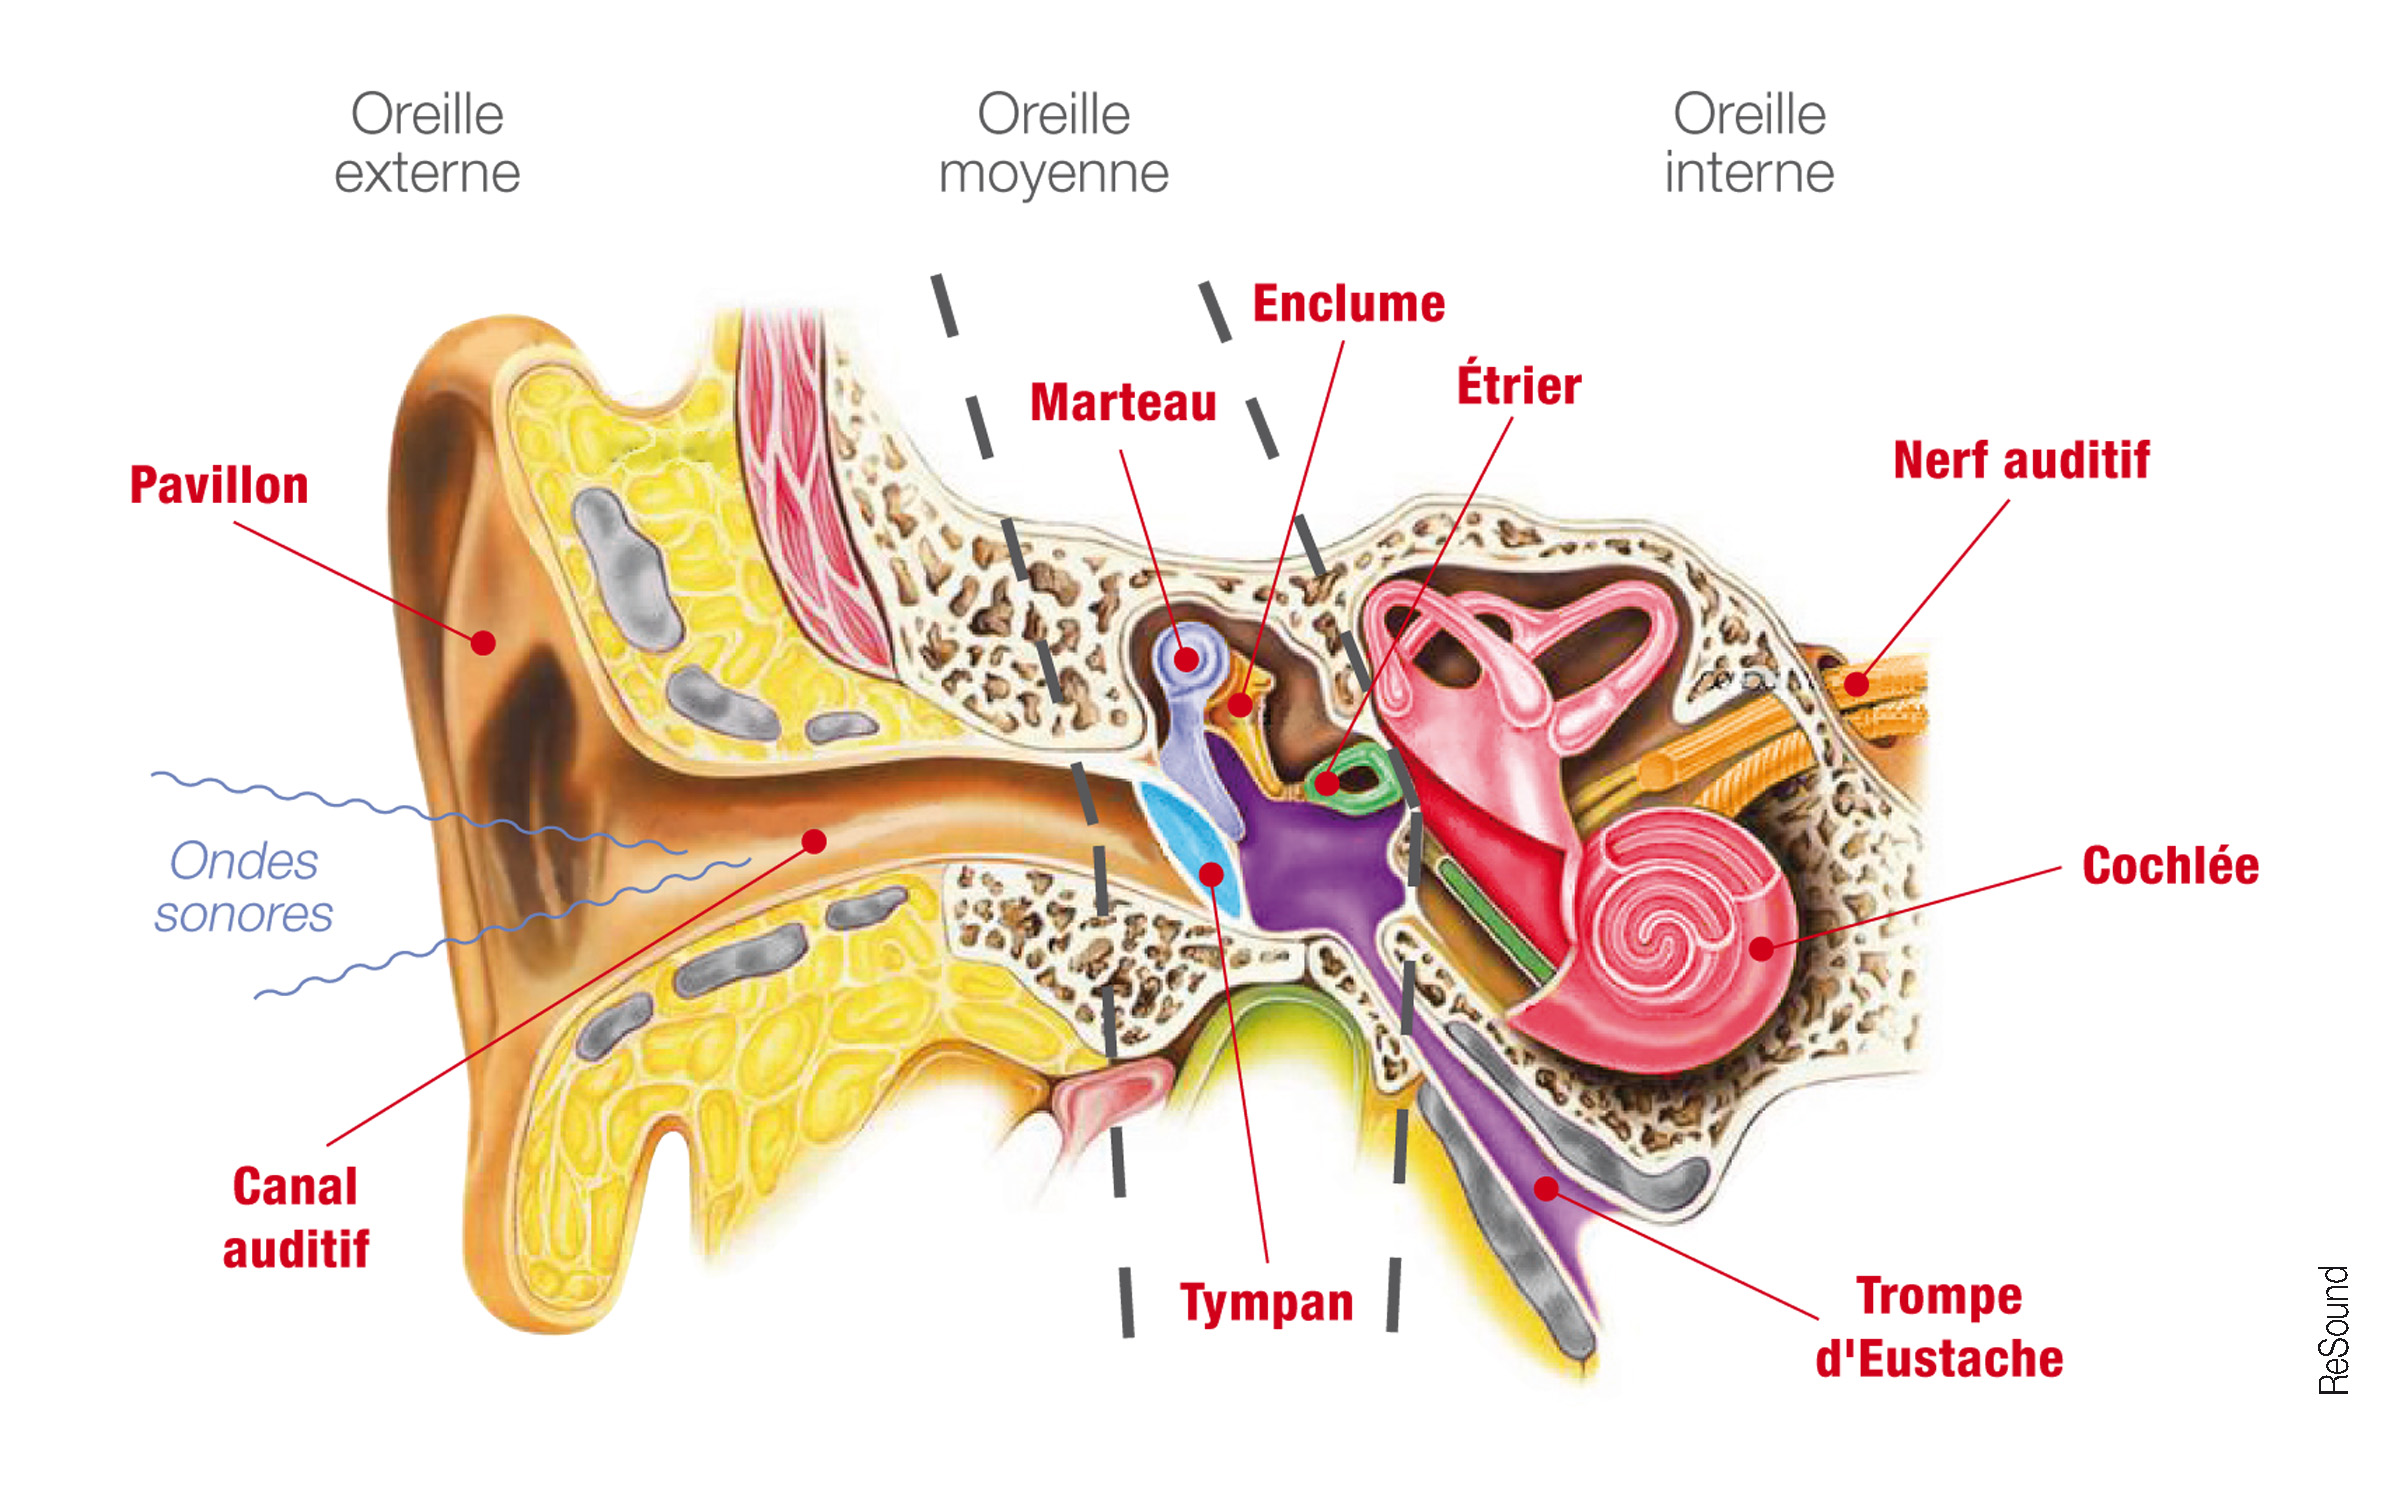
\includegraphics[width=0.8\textwidth]{../../../../Pictures/OREILLE.jpg}
% \caption[width=0.5\textwidth]{Schéma de l'oreille interne (http://www.mon-audition.info/wp-content/uploads/2015/01/OREILLE.jpg)}
% \label{fig:schemaOreille}
%\end{figure}
  
L'oreille humaine est composé de trois parties ayant chacune leur fonction : l'oreille externe  qui permet la localisation des sources, l'oreille moyenne qui joue le rôle d'amplification du son et l'oreille interne qui traduit la pression acoustique du signal en un signal électrique interpréter par le cerveau. Si le tympan et les osselets jouent le rôle d'adaptateur d'impédance entre l'extérieur et l'oreille interne, c'est la cochlée qui permet d'obtenir un signal électrique qui sera transmise au cerveau via le nerf auditif. \\

%\begin{figure}[hbtp]
% \centering
% 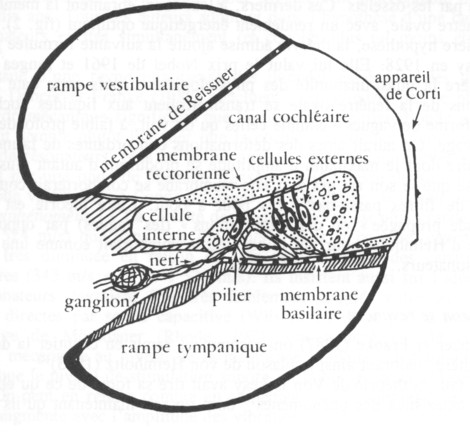
\includegraphics[width=0.4\textwidth]{../../../../Pictures/cochlea.jpg}
% \caption{Schéma en coupe d'une cochlée (http://auriol.free.fr/psychosonique/ClefDesSons/ecoute.htm)}
% \label{fig:schemaCochlé}
%\end{figure}

La cochlée consiste en une spirale creuse traversé par le canal cochléaire composé notamment de la membrane basilaire sur laquelle repose l'organe de Corti. Lorsqu'une onde acoustique arrive au tympan, elle est converti en énergie mécanique dont l'énergie est ensuite transmise à la cochlée grâce au osselets. Cette énergie met en mouvement la membrane basilaire à des positions localisées qui dépendent de la fréquence du signal. Par ce déplacement, les cellules cilié se trouvant dans l'organe de Corti vont alors bouger convertissant le signal mécanique en en signal électrique qui se propage ensuite jusqu'au cerveau à travers le nerf auditif (http://www.cochlea.eu/cochlee). C'est ensuite dans le cerveau que le son est interprété et que l'auditeur peut y mettre un sens. Pour cela, les évolution des caractéristiques acoustiques (niveau sonore, continuité temporelle et fréquentielle) du son aide à la compréhension et la distinction des sources présentes. \\

La CASA reprend donc ces éléments et cherche à traduire ces organes en étapes numériques, la première étant la modélisation de l'ensemble oreille externe/moyenne/interne.\\

\subsubsection{Analyse fréquentielle}

L'oreille externe et moyenne sont résumées en un simple filtre passe-haut. Ensuite, l'oreille interne est synthétisée par un filtrage cochléaire (cochléogramme). Ce filtre traduit la sélectivité fréquentielle de la membrane basilaire en la modélisant par une banque de filtres passe-bandes dans laquelle chaque filtre simule la réponse en fréquences d'un point particulier de la partition cochléaire. Les cellules ciliées étant les éléments dans la membrane qui transmettent les perturbations vers le nerf auditif, leur réaction est modélisée par un filtre de gammatone basé sur un filtre impulsionnel.\\

\begin{equation}
gt(t) = t^{n-1} e^{-2\pi bt } \cos(2\pi f_0 t+\phi)
\end{equation}

avec $t$, le temps en seconde, $n$, l'ordre du filtre, $f_0$, la fréquence centrale du filtre en Hz, $b$ la largeur de la bande passante en Hz et $\phi$ la phase (rad). En sortie de la cochlée, on préfère utilisé comme représentation temps-fréquence, un cochléogramme au spectrogramme qui permet de mieux mettre en évidence les basses fréquences grâce à une échelle logarithmique.\\

\subsubsection{Paramètre d'extraction}

Cette seconde étape vise à extraire plusieurs paramètres qui seront utile à l'étape de groupement (partie \ref{sec:groupement}) : 

\paragraph{Pitch et périodicité}
L'objectif consiste à déterminer les fréquences fondamentales et les phénomènes récurrent à partir de l'auto-corrélations $a(t,f,\tau)$ pour chaque oreille (corrélogramme) et de l'inter-corrélation $c(t,f,\tau)$ entre les signaux des deux oreilles $h_L$ et $h_R$(corrélogramme-croisé). 

\begin{equation}\label{eq:CASA_FAC}
a(t,f,\tau) = \sum h(t-n,f)h(t-n-\tau,f)w(n), 
\end{equation}

\begin{equation}\label{eq:CASA_FAC}
c(t,f,\tau) = \sum h_L(t-n,f)h_R(t-n-\tau,f)w(n).
\end{equation}

La somme pour chaque fréquence permet alors de déterminer les fréquences fondamentales présentes

\begin{equation}
A(t,\tau) = \sum_f a(t,f,\tau),
\end{equation}
\begin{equation}
C(t,\tau) = \sum_f c(t,f,\tau).
\end{equation}

Si plusieurs sources sonores sont simultanées et présente des différentes fréquences fondamentales, il existe un moyen pour les déterminer \cite{DeCheveigne20006}.
\paragraph{Corrélation croisée des voix}
Comme les réponses des filtres gammatone se recouvrent, plusieurs bandes peuvent réagir à une même harmonique. La corrélation autour des fréquences voisines permet alors de mieux connaitre le phénomène. celle-ci se définit comme l'inter-correlation au fréquences voisines des auto-corrélation normalisées. 
\begin{equation}
k(t,f) = \frac{1}{M}\sum_{\tau=0}^{M-1}\hat{a}(t,f,\tau) \hat{a}(t,f+1,\tau)
\end{equation}
\paragraph{Variation de l'intensité}
L'apparition ou la disparition de sources sonores pouvant d'accompagner d'une variation du niveau sonore. Des valeurs seuils sont déterminées pour détecter ces variations à partir de la dérivée de l'enveloppe du signal.

\paragraph{Modulation d'amplitude}
L'extraction des modulation d'amplitude des enveloppes permet de revenir à l'enveloppe du signal même. Une des méthodes couramment employé est l'utilisation des transformée de Hilbert ou bien l'amplitude absolue des signaux en sortie des filtres complexes de gammatone.

\paragraph{Modulation de fréquence}
Ce paramètre permet de rendre compte des régimes transitoires.  Deux techniques existent, la première méthode consiste revient à extraire les contours spatiales du cochléogramme, la seconde implique de calculer la réponse fréquentielle instantanée des signaux en sortie des filtres passe-bandes. 

\subsubsection{Représentation à niveau moyen}
Cette étape consiste à établir une représentation des paramètres précédents le plus souvent par segmentation. 
\subsubsection{Groupement des sources}\label{sec:groupement}

\subsubsection{Re-synthétisation}



La cartographie du signal permet ensuite de retrouver le signal perçu par l'auditeur. Elle se base sur des fonctions de corrélations (corrélogramme) visant à synthétiser les phénomènes de masquage et à faire ressortir les pics principaux des signaux
Enfin un second corrélogramme entre les signaux issus des deux microphones (simulant les deux oreilles) permettent la localisation des sources grâce à leur déphasage. La séparation des différentes sources se fait lors du cochléogramme à partir d'un masque binaire. Ce masque est généré par le spectrogramme de la source ciblé seul  puis pondère chaque trame \og temps-fréquence \fg{} du cochléogramme afin de ne conserver que la source souhaitée.\\

C'est donc une approche \textit{bottom-up} où d'un signal complexe on détermine l'ensemble des sources présentes.  Cette méthode est le plus souvent utilisée pour la séparation de signaux de paroles ou de musique \cite{BrownCASASpeech}, c'est-à-dire d'un signal harmonique et n'est donc pas adaptée pour celle de sons environnementaux plus complexes où la présence de contenus harmoniques est quasi inexistante. C'est donc une méthode très peu employée pour ces ambiances sonores.

\subsection{Les méthodes par dictionnaires}

\subsubsection{Analyse en Composantes Indépendantes}\label{part:ACI}

L'Analyse en Composantes Indépendantes (ACI) \cite{Herault} \cite{Comon} est une méthode appartenant aux méthode dite \textit{séparation de sources en aveugles}, c'est-à-dire qui sépare un ensemble de sources sonore d'une mixture sans (ou avec peu) informations sur celles-ci. Le plus souvent, cela équivaut à résoudre un problème sous déterminé. Le principe de la méthode consiste, à partir d'un réseau de capteurs, à trouver les sources présentes dans un signal audio en supposant leur indépendances les unes des autres. \\

L'illustration la plus couramment citée pour cette méthode est l'effet \og cocktail party \fg{} \cite{Cherry}. Cet effet résume la capacité de l'être humain à séparer la voix de l'interlocuteur avec qui il discute d'un flux sonore environnant bruyant composé d'autre discussions. Cette habilité est notamment permise par l'indépendance entre le signal \textit{voix} et le bruit ainsi que par l'écoute binaural du sujet. \\

L'ACI consiste alors à décrire les signaux de chaque capteur $x_n$ comme une combinaison linéaires des sources $s_n$ présentes, supposées indépendantes et pondérées par des effets propagatifs $a_{nn}$. Dans le cas du \og cocktail party \fg{}, on considère deux signaux (la voix et le bruit) où les capteurs sont les deux oreilles de l'auditeur. 

\begin{subequations}\label{eq:ACI1}
\begin{align}
x_1 &= a_{11} s_1 + a_{12} s_2 + \dots + a_{1N} s_N\\
x_2 &= a_{12} s_1 + a_{22} s_2 + \dots + a_{sN} s_N\\
x_n &= a_{n1} s_1 + a_{n2} s_2 + \dots + a_{nN} s_N
\end{align}
\end{subequations}

Le système \ref{eq:ACI1} est alors généralisé à un ensemble $N$ de sources par l'équation~(\ref{eq:ACI2}).

\begin{equation}\label{eq:ACI2}
\mathbf{x} = \mathbf{As}
\end{equation}

où $\mathbf{x}$ est de dimension $P \times 1$ comprenant l'ensemble des mesures réalisées par les capteurs, $\mathbf{s}$, de dimension $N \times 1$, résume les différentes sources présentes et $\mathbf{A}$, de dimension $P \times N$, une matrice déterministe résumant les aspects de propagation entre les sources et les capteurs. Cet aspect peut se révéler très intéressant lorsque les milieux dans lesquels évoluent les signaux sont complexes. Toutefois, l'estimation de la matrice $\mathbf{s}$ ne peut se faire que si le nombre de capteurs est égale ou supérieur aux nombres de sources présentes ($P \geq N$).\\

Le problème à résoudre devient alors

\begin{equation}
\text{min } I(\mathbf{A}^{-1}\mathbf{x})
\end{equation}

où $I(\mathbf{y})$ est une mesure de dépendance des coordonnées de la matrice $y$. Sa minimisation assure la meilleure indépendance possible des solutions du problème.
Il y a indépendance entre les sources lorsque 
\begin{equation}
p(\mathbf{x}) = \prod_{i = 1}^N p(x_i).
\end{equation}
où $p(\mathbf{x})$ est une fonction de densité de probabilité de $\mathbf{x}$. La mesure d'indépendance est ensuite déterminée par le calcul de la divergence de Kullback-Leibler que Comon \cite{Comon} a choisi en raison de ces propriétés.

\begin{equation}\label{eq:divKLICA}
D(\mathbf{y}) = \int p(\mathbf{y})\log\frac{p(\mathbf{y})}{\prod_{i = 1}^N p(y_i)} d\mathbf{y}.
\end{equation}

La minimisation de (\ref{eq:divKLICA}) rend alors les composantes moins dépendantes les unes des autres. Toutefois, il n'existe pas d'algorithme générique qui permettrait de résoudre le problème facilement \cite{CichockiICA}, des connaissances \textit{a priori} sur les sources ou sur l'environnement sont nécessaires pour exprimer au mieux l'indépendance comme l'évolution temporelle ou spatiale des signaux.  \\

L'application de cette méthode est prévue pour l'analyse et la compression de données, la détection bayesienne, la localisation de sources et enfin l'identification et la déconvolution de signaux en aveugles.\\

Si la technique peut sembler intéressante elle présente l'inconvénient de nécessiter un nombre de capteur égal ou supérieur au nombre de sources présentes. Dans un espace clôt, cette condition est supportable mais, dans le cadre urbain où le nombre de sources est important, cette contrainte rend son utilisation peu envisageable.\\

Les méthodes de séparation couramment utilisées ne sont donc pas des méthodes bien adapté à notre situation et ne peuvent donc pas être utilisé. Néanmoins, une autre technique appartement à la méthode de \textit{BSS} offre des résultats intéressant et prometteur et peut être envisagée pour des ambiances sonores urbaines : la Factorisation en Matrice Non-Négative.

%\subsection{Applications}
%
%L'utilisation de ces techniques dans le domaine de la classification et de la détection se fait couramment et dans des domaines diverses (
%
%Rappeler les applications diverses dans les images, le milieu médicale, textuelles.
%Dans le cadre des signaux audiophoniques :
%séparation des sources sonores afin de réaliser des commandes vocales, de restaurer des signaux audio indépendamment 
%paroles, musiques, sons environnementaux...
%
%Dans le cadre de la restauration audio, classifier par genres musicaux, artistes..., traitement actif du son également, reconnaissance ou commande vocale.
%Les sons environnementaux sont constitués des sons qui ne sont ni musicaux ni de la paroles. On trouve dedans les sons produits par l'Homme (bruit mécaniques) ou ceux produit par les animaux (bio-acoustique). Ce choix de distinctions provient de la nature des sons qui est beaucoup plus harmonique dans la parole et la musique que dans l'environnement.\\
%
%Dans le cadre des sons urbains, on trouve des études portant sur la reconnaissance des sons présents en ville (Defréville, Couvreur)

%\bibliographystyle{unsrt}
%\bibliography{../bibliographie}

%\end{document}
\chapter{La Factorisation en Matrices Non-négatives}
\label{chap:NMF}

\section*{\centering Résumé}


\noindent{\small \textbf{
Le fonctionnement de la Factorisation en Matrices Non-négatives (NMF) est présenté dans ce chapitre. Cette méthode consiste à approximer le spectrogramme en amplitude d'un signal audio par le produit de deux matrices positives : $\mathbf{W}$, un dictionnaire composé de spectres audio, et $\mathbf{H}$, la matrice d'activation temporelle. Les différents aspects de son fonctionnement sont décrits : familles de divergences, algorithmes de mise à jour des matrices, méthode d'apprentissage du dictionnaire. Une forme de NMF est également proposée : la NMF \textit{initialisée seuillée} où un dictionnaire, appris sur la source d'intérêt, est mis à jour et dont les éléments relatifs à cette source sont ensuite sélectionnés par une technique de seuillage. Enfin, les différentes contraintes, qui peuvent être apposées sur les matrices de la NMF, sont décrites et notamment la contrainte de régularité temporelle et de parcimonie.}}

\vspace{2cm}

La Factorisation en Matrices Non-négatives étant la méthode retenue pour la suite des travaux, ce chapitre en présente son fonctionnement. Les principes généraux sont dans un premier temps détaillés, puis les différentes approches de cette méthode sont explicitées.

\section{Principe de fonctionnement de la Factorisation en Matrice Non-négatives}
La Factorisation en Matrices Non-négatives (abrégé NMF pour \textit{Non-negative Matrix Factorization} en anglais) est une technique d'approximation linéaire visant à décomposer une matrice $\textbf{V}$ non-négative de dimensions $F \times N$ en un produit de deux matrices tel que

\begin{equation}
\textbf{V} \approx \textbf{WH}
\end{equation}

où $\textbf{W}$ et $\textbf{H}$ sont deux matrices, également non-négatives, de dimensions respectives $F \times K$ et $K \times N$, appelées \textit{dictionnaire} et \textit{matrice d'activation}. Le choix du rang de factorisation $K$ est le plus souvent déterminé afin que la relation $F \times K + K \times N << F \times N$ soit respectée. Dans ce cas, la NMF est une méthode d'approximation dite de faible rang car elle permet la réduction de la dimensionalité des données. 

La contrainte de non-négativité permet d'assurer seulement des combinaisons additives, la soustraction d'information n'est pas possible dans le produit $\mathbf{WH}$. Cela assure ainsi que les éléments du dictionnaire appartiennent bien tous au même domaine non-négatif que les données d'observations $\mathbf{V}$, et donc de leur interprétabilité. En cela, la NMF réalise alors une représentation dite \og par partie \fg{} dans laquelle $\mathbf{W}$ est composée de briques élémentaires qui, additionnées, permettent d'approximer l'ensemble de $\mathbf{V}$. Un exemple de NMF est présenté dans la Figure \ref{fig:ex_NMF}. Chaque colonne $n$ de la matrice $\mathbf{V}$ est décrite comme la somme des éléments de $\mathbf{W}$ pondérés par la colonne $n$ de la matrice $\mathbf{H}$ :

\begin{equation}\label{eq:nmf_h}
\mathbf{v} \approx \mathbf{\tilde{v}} =  \mathbf{Wh}
\end{equation}

où les caractères minuscules représentent des vecteurs colonnes et $n$ est une trame temporelle. Les majuscules dénotent des matrices.

\begin{figure}[t]
\centering
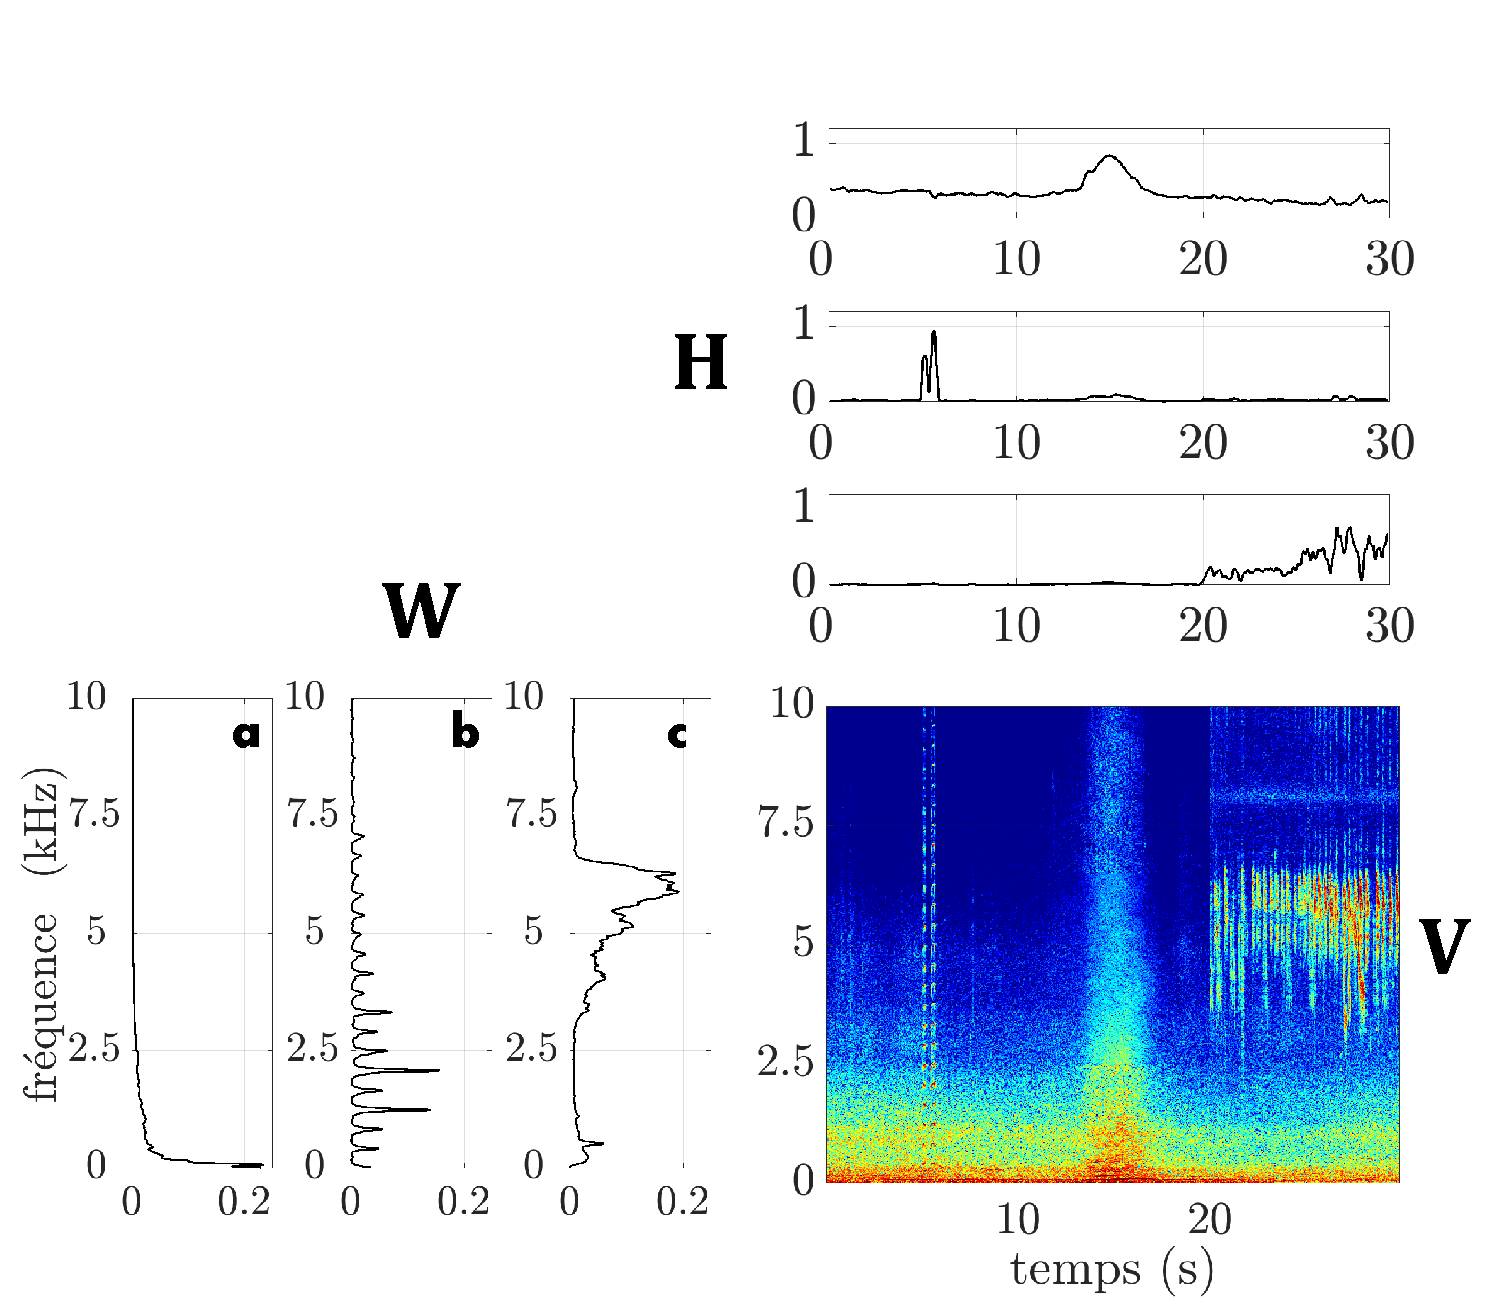
\includegraphics[width=.5\textwidth]{./figures/NMF/schema_introduction_nmf_fr.pdf}
\caption{Exemple d'une NMF pour un signal audio de mixture urbaine composé de 3 sources sonores. $\mathbf{W}$ et $\mathbf{H}$ sont constitués de 3 bases (K = 3) : a) un spectre voiture, b) un spectre de klaxon, c) un spectre d'oiseau.}
\label{fig:ex_NMF}
\end{figure}


Cette méthode est assimilable aux méthodes de factorisation comme l'Analyse en Composantes Principales (ACP), où la contrainte de non-négativité est remplacée par une contrainte d'orthogonalité entre les matrice $\mathbf{W}$ et $\mathbf{H}$, ou l'Analyse en Composantes Indépendantes (ACI) où l'indépendance entre chaque composante est supposée et où il est possible d'obtenir des valeurs négatives. \\

Si la NMF fut introduite pour la première fois par Paatero et Tapper \cite{paatero_positive_1994} en 1994 (mais sous le nom de \textit{Positive Matrix Factorization}), elle doit sa popularité aux travaux de Lee et Seung \cite{lee_learning_1999} dont les résultats furent publiés dans la revue \textit{Nature} en 1999. La NMF a ensuite trouvé de nombreuses applications dans des domaines variés : imagerie \cite{guillamet_introducing_2003, monga_robust_2007}, traitement de texte \cite{xu_document_2003, berry_email_2005}, biologie \cite{gao_improving_2005, chen_constrained_nodate}, gastronomie \cite{hawkins_clustering_2006} ou bien encore pour la recommandation de contenus audio-visuels \cite{luo2014efficient}. Dans le domaine de l'audio, c'est Smaragdis et Brown \cite{smaragdis_non-negative_2003} qui furent les premiers à l'utiliser dans le cas de la transcription d'un morceau de musique polyphonique. Plus généralement, pour un signal audio quelconque, la NMF consiste à approximer son spectrogramme en amplitude ou en puissance, obtenu, par exemple, à partir d'une Transformée de Fourier à Court Terme, à l'aide du dictionnaire $\textbf{W}$ constitué d'un ensemble de spectres sonores dont leurs amplitudes sont pondérées temporellement par les activateurs $\textbf{H}$.

De nombreuses applications de la NMF furent trouvées pour des signaux musicaux et contenant de la parole pour les tâches de détections \cite{dessein2013real}, de reconnaissances de sources \cite{gemmeke2013exemplar}, de classifications \cite{benetos2006musical}, de débruitage \cite{wilson_speech_2008} et de séparations de sources sonores \cite{virtanen_monaural_2007}.
Dans le cas de sons environnementaux (c'est-à-dire les sons qui ne sons ni musicaux ni de paroles), plusieurs applications ont été faites de la NMF. \cite{gemmeke2013exemplar} utilise la NMF en vue de réaliser de la détection d'évènements sonores sur des sons d'intérieurs (bruit de clés, sonnerie de téléphone, bruit de clavier\dots{}) et est testée sur une base de données synthétique où les évènements sonores sont artificiellement mixés à un bruit de fond, à des niveaux sonores calibrés. \cite{mesaros_sound_2015} réalise également de la détection de sons environnementaux. Un aspect intéressant de leur étude est la comparaison des performances de leur outil à partir de la forme du dictionnaire selon les techniques de réduction de dimensions employées. Ils comparent le cas d'un dictionnaire composé de bandes fines mais réduit en nombre d'éléments $K$ par un algorithme de clustering $K$-means et le cas d'un dictionnaire avec la base complète mais avec une représentation en bandes mel. Les auteurs observent alors que les deux techniques de réduction, sur leur corpus, offrent des performances similaires par rapport au dictionnaire original non réduit et suggèrent même la possibilité d'appliquer ces deux techniques de réduction en vue de réduire les tailles des matrices et ainsi réduire les coûts de calcul. Cet aspect sera repris pour la construction du dictionnaire dans la partie \ref{part:W_design}. Enfin, \cite{satoshi_innami_nmf-based_2012} ont proposé d'utiliser la NMF en vue de réaliser de la séparation de sources sur des mixtures sonores environnementales issues d'un processus de simulation. Leur méthode consiste dans un premier temps à isoler le bruit de fond des évènements sonores afin ensuite de les séparer individuellement. Pour cela, en plus d'une description des éléments par des MFCC, deux autres paramètres descripteurs sont ajoutés : la variance de l'élément $i$ sur la durée de la scène et son rapport des valeurs proches de zéro. Ces paramètres permettent de différencier les évènements sonores, dont ces valeurs seront alors élevées, du bruit de fond, où la variance et le rapport seront proches de zéro. Ces travaux sont toutefois, réalisés sur une base de données restreintes à quelques éléments audio.

\section{Fonction de coût et familles de divergences}

Le problème à résoudre lors d'une NMF est celui d'une minimisation où il faut trouver la combinaison optimale de $\mathbf{WH}$ qui sera la plus proche de $\mathbf{V}$. Cela se traduit mathématiquement par la relation \ref{eq:D(V-WH)} :

\begin{equation}\label{eq:D(V-WH)}
\text{min}~D\left(\textbf{V} \Vert \textbf{WH}\right) \quad \text{avec} \quad \mathbf{W} \geq 0, \mathbf{H} \geq 0.
\end{equation}

$D\left(\textbf{V} \vert\vert \textbf{WH}\right)$ est alors une mesure de similarité, appelée \textit{fonction de coût}, qui peut appartenir à différentes familles de divergences comme les divergences de Csiszar \cite{cichocki2006csiszar} et de Bregman \cite{bregman_relaxation_1967, dhillon_generalized_2005}. Cette dernière famille de divergences est la plus couramment utilisée dans le cadre de la NMF. Elle se définit, dans un sous-ensemble convexe $S$ d'un espace de Hilbert, comme :

\begin{equation}\label{eq:Bregdiv}
D_{\Phi}(\textbf{x}\vert\vert \textbf{y}) =
\mathbf{\Phi}(\mathbf{x}) - \mathbf{\Phi}(\mathbf{y}) -
\langle\mathbf{x}-\mathbf{y},\nabla\mathbf{\Phi}(\mathbf{y})\rangle
\end{equation}

où  $\mathbf{x} = (x_1, x_2, \dots x_N)$ et $\mathbf{y} = (y_1, y_2, \dots y_N)$ sont deux distributions, $\mathbf{\Phi}$ est une fonction continue dérivable et strictement convexe défini sur $\mathbb{R}^+$, $\nabla\mathbf{\Phi}(\mathbf{y})$ est le gradient de $\mathbf{\Phi}$ en $\mathbf{y}$ et $\langle .,.\rangle$ est le produit scalaire hermitien. L'équation~(\ref{eq:Bregdiv}) peut être décomposable élément par élément :

\begin{equation}
D_{\Phi}(\mathbf{x}\vert\vert \mathbf{y}) = \sum_{n=1}^N d_{\Phi}(x_n\vert y_n)
\end{equation}

avec $d_{\Phi}(x_n\vert y_n)$, la mesure de similarité entre deux scalaires et $\mathbf{\Phi(x)} = \sum_{n=1}^N \phi(x_n)$. L'équation \ref{eq:Bregdiv} se résume alors à une somme des divergences entre les composantes des distributions $\mathbf{x}$ et $\mathbf{y}$ :

\begin{equation}\label{eq:divBregWise}
D_{\Phi}(\textbf{x}\vert\vert \textbf{y}) = \sum_{n=1}^N \phi(x_n)-\phi(y_n)-\phi'(y_n)(x_n-y_n).
\end{equation}

La fonction de coût s'exprime donc comme la divergence de Bregman appliquée à chaque élément de $\mathbf{V}$ et $\mathbf{WH}$,

\begin{equation}\label{eq:similarite2}
D\left(\textbf{V} \vert\vert \textbf{WH} \right) = \sum_{f = 1}^{F} \sum_{n = 1}^{N} d_{\phi}
\left(\textbf{V}_{fn} \vert \left[ \textbf{WH} \right]_{fn} \right).
\end{equation}


Cette divergence possède plusieurs propriétés :

\begin{enumerate}
\item \textbf{Non-négativité} : $d_{\phi}(x\vert y) \geq 0$.

\item \textbf{Séparabilité} : si $d_{\phi}(x\vert y) = 0$ alors $x = y$.

\item \textbf{Convexité} : $D_{\phi}(\textbf{x}\vert\vert \textbf{y})$ est une fonction réelle strictement convexe pour le 1\ier{} argument mais pas nécessairement pour le second.

\item \textbf{Linéarité} : pour deux fonctions convexes, réelles $\phi_1$ et $\phi_2$,  $d_{\alpha \phi_1 + \beta \phi_2}(x\vert y) = \alpha d_{\phi_1}(x\vert y)+\beta d_{\phi_2}(x\vert y)$ où $\alpha$ et $\beta \in \mathbb{R}^+$.

\item \textbf{Dualité} : pour la fonction convexe conjuguée $\phi^{\ast}$, $d_{\phi^{\ast}}(y^{\ast}\vert x^{\ast}) = d_{\phi}(y \vert x)$.
\end{enumerate}

Si la propriété de non-négativité en fait une famille adaptée pour la NMF, celle de convexité implique qu'il n'est possible que de déterminer un minimum local et donc pas nécessairement la solution exacte au problème énoncé.

\section{Une sous-classe des divergences de Bregman : la $\beta$-divergence}

Dans \cite{banerjee2005clustering}, les auteurs démontrent qu'à chaque divergence de Bregman est associée une famille exponentielle unique $p\left(x\vert \theta,\lambda\right)$:

\begin{align}
 \label{eq:modele_disp_exp}
p\left(x\vert \theta,\lambda\right) &= h(x,\lambda) \exp\left[\lambda^{-1}\left(\theta(y) x-\psi(\theta) \right)\right],\\
 &= g(x,\lambda) \exp\left(-\lambda^{-1} d_{\phi}(x\vert y) \right),  \label{eq:tweedie_breg}
\end{align}

avec $h(x,\theta) $, la fonction de base, $\theta(y)$, le paramètre normal (ou canonique), $\lambda$, celui de la dispersion, $\psi(\theta)$ celui de la normalisation et $g(x,\lambda) = h(x,\lambda)\exp(\lambda^{-1}\phi(x))$. Les paramètres sont reliés entre eux par plusieurs relations $y(\theta) = \frac{d\varphi(\theta)}{d\theta}$, $\theta (y) = \frac{d\phi(y)}{dy}$ et $\frac{d\theta (y)}{dy} = v(y)^{-1}$. Un cas remarquable de distribution est la distribution de Tweedie \cite{jorgensen_exponential_1987} qui relie la variance $v(x)$ à la moyenne (ou espérance) de la distribtion $x$ par une relation polynomiale \cite{yilmaz_alpha/beta_2012} définie par un paramètre de forme $\beta$,

\begin{equation}
v(x) = x^{2-\beta}.
\end{equation}

L'ensemble des divergences de Bregman définies par cette distribution dans l'équation \ref{eq:tweedie_breg} est alors paramétré par le choix de cette valeur $\beta$ et peut être généralisé :

\begin{subequations}\label{eq:divBetaGenerale}
\begin{numcases}{d_{\phi_{\beta}}(x\vert y) =}
    \frac{1}{\beta(\beta-1)}(x^{\beta}+(\beta-1)y^{\beta}-\beta xy^{\beta-1}), & $\beta \in \mathbb{R} \backslash \lbrace 0,1\rbrace$,\label{eq:def_beta}\\
    \dfrac{x}{y}-\log \dfrac{x}{y}-1, & $\beta = 0$,\label{eq:def_divIS}\\
    x\log \dfrac{x}{y} - x + y, & $\beta = 1$.\label{eq:def_divKL}
\end{numcases}
\end{subequations}

Les équations \ref{eq:def_divIS} et \ref{eq:def_divKL} sont des cas limites de l'expression \ref{eq:def_beta}. Chaque paramètre de forme choisi coïncide alors avec une distribution particulière des données : pour $\beta = 1$, la distribution de Tweedie s'apparente à une distribution de Poisson, pour $\beta = 0$, c'est une distribution gamma (ou exponentielle). Dans le cas où $\beta = 2$, cela correspond à la distribution de la loi normale (ou loi de Gauss) de moyenne $\mu$ et de variance $\sigma^2$ :

\begin{align}
p(x \vert \theta, \lambda) & = \frac{1}{\sqrt{2 \pi \sigma^2}}\exp\left(-\frac{1}{2} \left(\frac{x-\mu}{\sigma} \right)^2 \right),\\
& = \frac{1}{\sqrt{2 \pi \sigma^2}}\exp\left(-\frac{1}{\sigma^2}  d_{\phi_{2}}(x\vert \mu) \right)
\end{align}

avec $g(x,\lambda) = \frac{1}{\sqrt{2 \pi \sigma^2}}$, $\lambda = \sigma^2$ et $d_{\phi_{2}}(x\vert \mu)$ qui correspond alors à la distance Euclidienne. Ces distances et divergences, déduites de la distribution de Tweedie, sont alors regroupées dans une sous-classe des divergences de Bregman, appelée $\beta$-divergences \cite{hennequin_beta-divergence_2011}. C'est cette famille de divergences qui est la plus couramment utilisée dans le cadre de la NMF. La Figure \ref{fig:allure-divergence} permet d'illustrer le comportement de ces divergences. Dans le cas où $\beta \in \left[ 1,2 \right]$, on constate que $d_{\phi_{\beta}}$ est strictement convexe. En dehors de cet intervalle, les divergences présentent également une partie concave. \\

\begin{figure}[h]
\centering
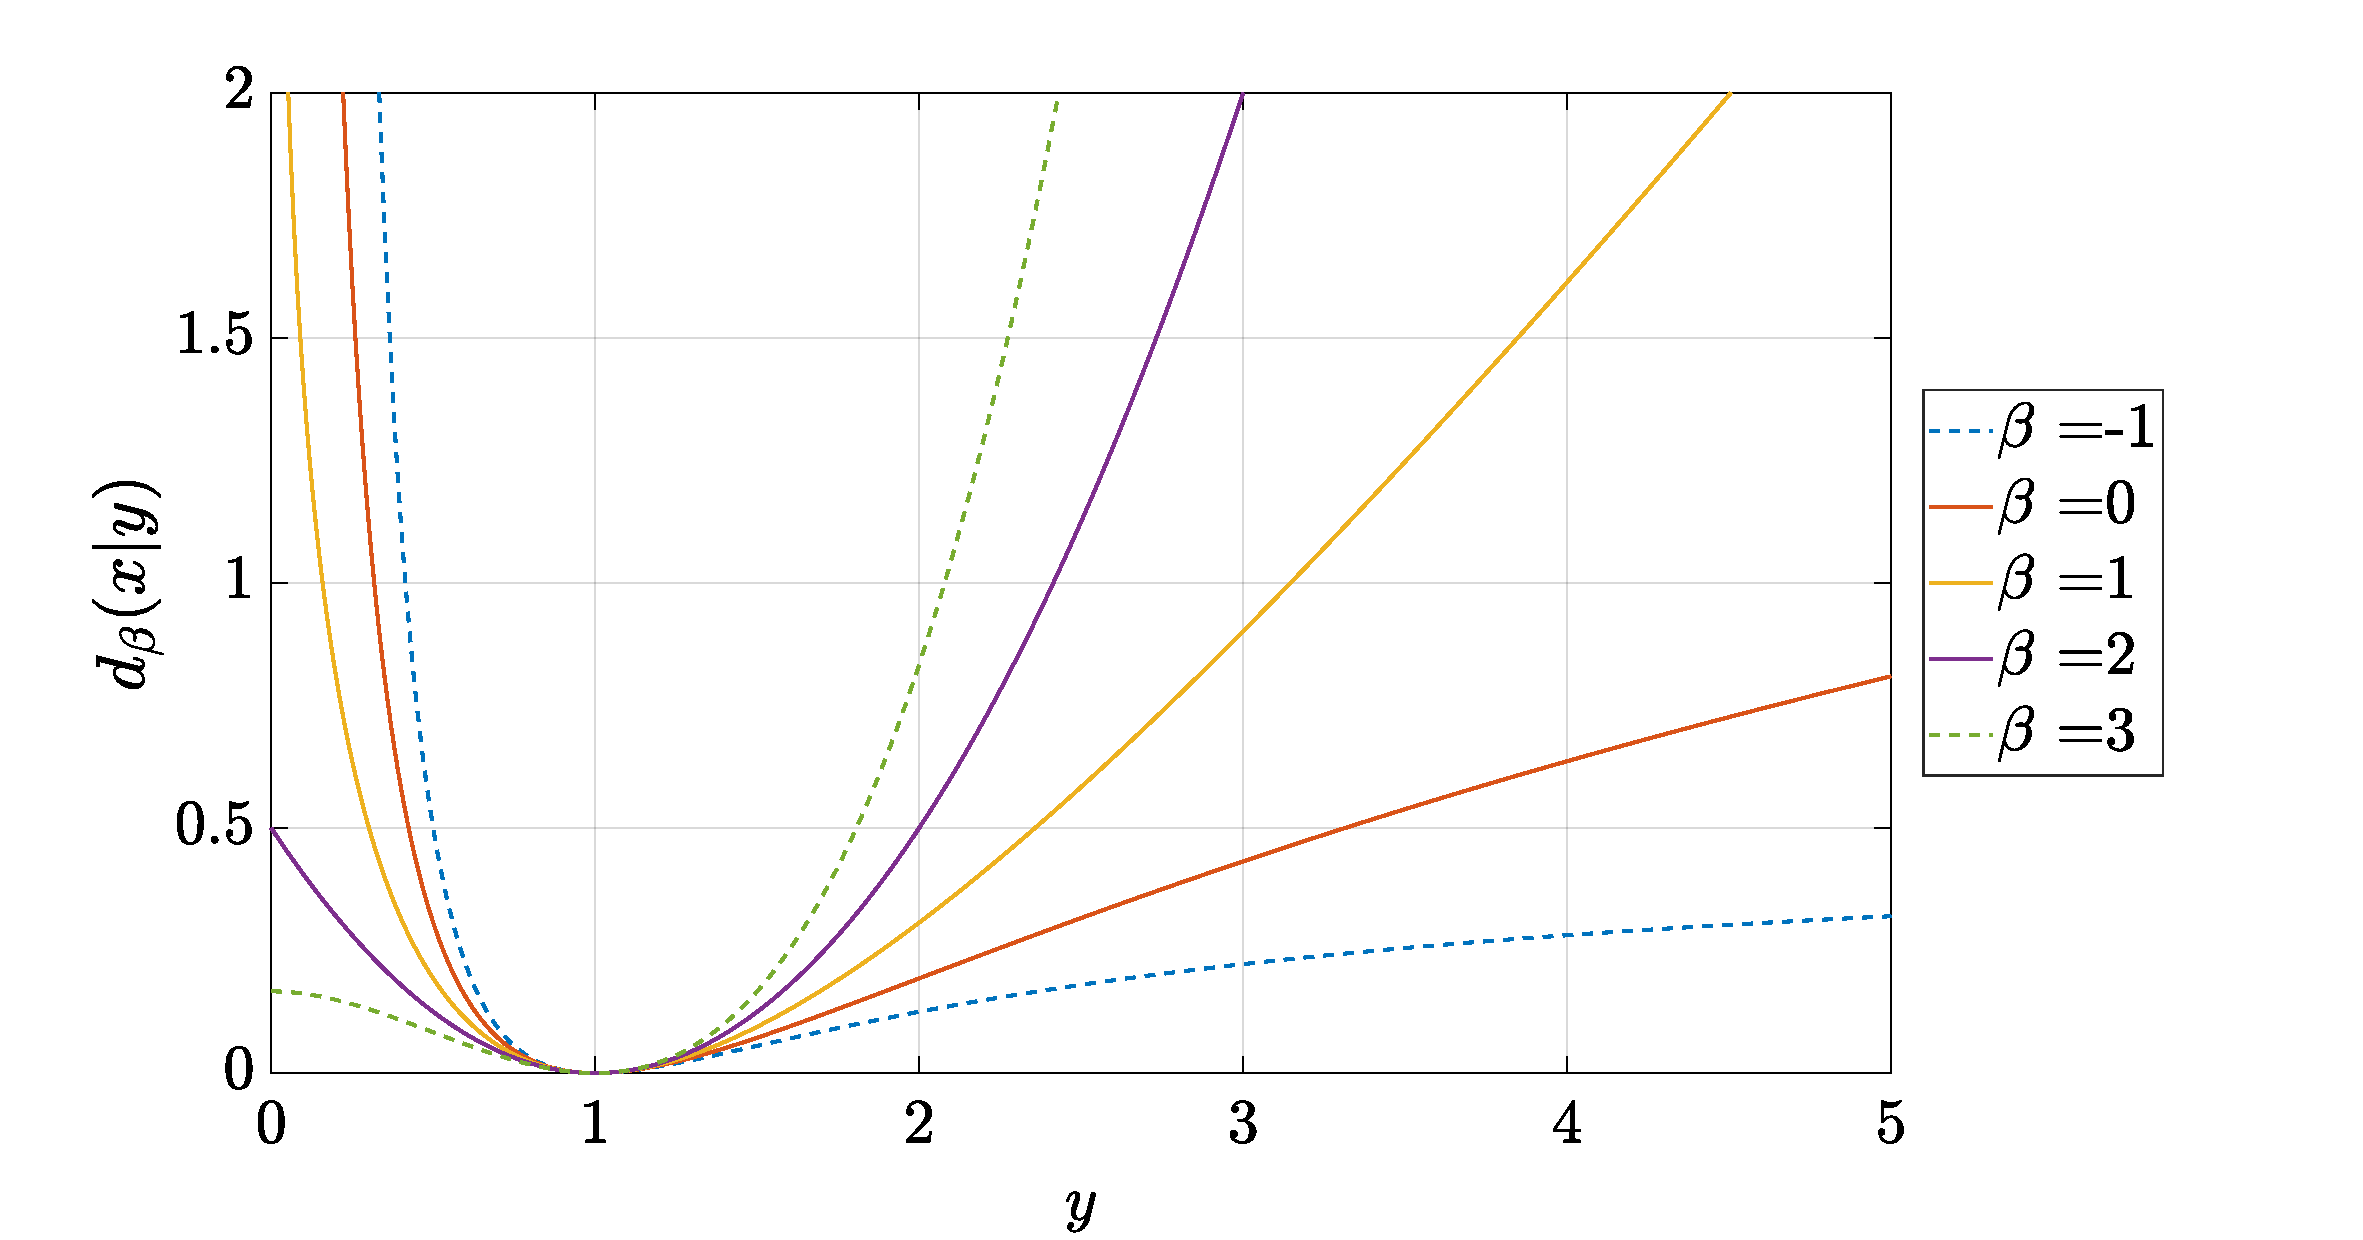
\includegraphics[width=.7\textwidth]{./figures/NMF/betaDiv_exemple.pdf}
\caption{Évolution des $\beta$-divergences pour un cas simple ($x$ = 1).}
\label{fig:allure-divergence}
\end{figure}

Dans le reste du document, par soucis de clarté, les $\beta$-divergences $d_{\phi_{\beta}}$ seront dénommées $d_{\beta}$. Trois $\beta$-divergences associées à des valeurs spécifiques de $\beta  = [0,1,2]$ et à des distributions particulières, sont le plus souvent utilisées dans le cadre de la NMF et sont présentées dans les parties suivantes.

\subsection{Distance Euclidienne}\label{part:dist_EUC}
Lorsque $\beta = 2$, la $\beta$-divergence devient \textbf{la distance Euclidienne} (abrégé EUC) :

\begin{equation}
d_{{2}}(x\vert y) = \dfrac{1}{2}(x-y)^2.
\end{equation}

Cette métrique équivaut à une mesure de similarité entre les points $x$ et $y$ et se révèle très sensible aux grandes variations entre eux en raison de la présence de la puissance carré. En plus des propriétés des divergences de Bregman, la distance Euclidienne en possède 2 autres :
\begin{enumerate}

\item \textbf{Symétrie} : $d_{2}(x \vert y ) = d_{2}(y \vert x)$.

\item \textbf{Inégalité triangulaire} : $d_{2}(x \vert y ) \leq d_{2}(x \vert z ) + d_{2}(x \vert z )$.\\
\end{enumerate}

Comme chaque mesure de distance au point $(x,y)$ possède le même poids que les autres couples de points, il est possible, pour la distance Euclidienne, de considérer une pondération $g_{v_{fn}}$  sur les distances selon un critère psycho-acoustique, liée à l'énergie de $v_{fn}$. Cette pondération permet de prendre en compte dans l'erreur de reconstruction, les points temps-fréquences de faibles énergies \cite{virtanen2004separation} :

\begin{equation}
d'_2(v_{fn} \vert w_{fk} h_{kn}) = g_{v_{fn}} d_2 (v_{fn} \vert w_{fk} h_{kn}).
\end{equation}

\subsection{Divergence de Kullback-Leibler}\label{part:div_KL}
L'expression \ref{eq:def_divKL} correspond à \textbf{la divergence de Kullback-Leibler} (abrégé K-L) \cite{kompass_generalized_2007, cichocki_new_2006} . Elle traduit comment une densité de probabilité $\mathbf{x}$ diverge d'une seconde distribution $\mathbf{y}$. En d'autres termes, c'est une mesure de l'information perdue lorsque $\mathbf{y}$ est utilisée pour approximer $\mathbf{x}$. Ne respectant pas les propriétés de symétrie et d'inégalité triangulaire, elle n'est donc pas une distance. La divergence K-L est un cas remarquable puisqu'elle appartient à la fois aux divergences de Bregman et à une autre famille de divergences, les divergences de Csiszar \cite{cichocki_csiszars_2006}.

\subsection{Divergence d'Itakura-Saïto}\label{part:div_IS}
L'expression \ref{eq:def_divIS} est celle de \textbf{la divergence d'Itakura-Saïto} (abrégé I-S) \cite{itakura1968analysis, bertin_les_2009}. Cette divergence est la seule des $\beta$-divergences à posséder la propriété d'\textit{invariance d'échelle} :

\begin{equation}\label{eq:scale_IS}
d_{0}(\lambda x \vert \lambda y) = d_{0}(x \vert y).
\end{equation}

Ce rapport signifie que le même poids est attribué entre les fortes et les faibles valeurs de $\mathbf{x}$. Ainsi, la divergence aux faibles puissances sonores entre $\textbf{V}$ et $\textbf{WH}$ aura la même importance que dans les fortes puissances. La relation \ref{eq:scale_IS} est généralisable à l'ensemble des $\beta$-divergences,

\begin{equation}
d_{\beta}(\lambda x \vert \lambda y) = \lambda^{\beta}d_{\beta}(x \vert y).
\end{equation}


Dans le cas où $\beta > 0$, la divergence est plus influencée par les composantes de fortes amplitudes. À l'inverse, dans le cas où $\beta < 0$, les composantes ayant une faible amplitude ont une plus grande prépondérance. Cette particularité, d'après \cite{fevotte_nonnegative_2009}, est intéressante dans le cadre de signaux audio, et notamment celui des signaux audio musicaux qui possèdent une forte dynamique et dont la puissance décroit exponentiellement en fonction de la fréquence. Une faible valeur de $\beta$ permet alors de mieux prendre en compte les composantes de moindres amplitudes dans la reconstruction du signal.

\subsection{Autres familles de divergences}
Si on s'est attardé à décrire longuement les $\beta$-divergences, d'autres familles de divergences peuvent être utilisées pour la NMF notamment celles appartenant aux divergences de Csiszar (ou appelées $f$-divergences). Cette famille est toutefois moins utilisée que celle de Bregman. Elle se définit comme

\begin{equation}
D_{\Psi} (\mathbf{x} \Vert\mathbf{y}) = \mathbf{x} \mathbf{\Psi} \left( \frac{\mathbf{x}}{\mathbf{y}}\right).
\end{equation}

Elle intègre notamment la distance de variation totale ($\psi(x) = \frac{1}{2}\vert x-1 \vert $), la divergence $\chi^2$ ($\psi(x) = (x-1)^2$), la distance d'Hellinger ($\psi(x) = (\sqrt{x}-1)^2$), les divergences $\alpha$ d'Amari $(\psi(x) = \frac{4}{1-\alpha^2} \left(1-x^{(1+\alpha)/2} \right))$ et la divergence de Kullback-Leibler ($\psi(x) = x\log (x)$). Elle possède plusieurs propriétés (non-négativité, unicité de la solution, symétrie, convexité, dépendance) qui sont détaillées dans \cite{csiszar2004information}.
Enfin, une proposition de généralisation des familles de divergences peut être trouvée dans \cite{cichocki_generalized_2011} où les auteurs généralisent les $\alpha$ et les $\beta$-divergences à travers l'équation  \ref{eq:expression_gen_alpha_beta} :

\begin{equation}\label{eq:expression_gen_alpha_beta}
D_{a, b}(x \vert y) = -\frac{1}{a b}\left(x^{a}y^{\beta}- \frac{a}{a+b}x^{a + b}-\frac{b}{a+b}y^{a+b} \right).
\end{equation}

Les valeurs des coefficients $a$ et $b$ permettent alors d'obtenir soit des $\beta$-divergences ($a = 1$) ou des $\alpha$-divergences ($a+b = 1$) mais également de nouvelles divergences. L'intérêt est d'étendre les familles et les divergences, afin de déterminer de nouveaux algorithmes de mise à jour dont les convergences peuvent être plus rapides, et d'offrir de nombreuses fonctions coûts pouvant mieux s'adapter au problème initial rencontré. Dans le cadre de ce travail, nous nous restreignons aux $\beta$-divergences en raison de leur popularité et des nombreux travaux dans la littérature qui s'y réfèrent.

Notons enfin qu'il n'est pas nécessaire de se restreindre aux divergences bien connues:  \cite{vincent2010adaptive} a, par exemple,  utilisé la NMF dans le cadre de la transcription de signaux musicaux et a déterminé un résultat optimal pour $\beta$ = 0,5. \\

\section{Mise à jour des formes de \textbf{W} et de \textbf{H}}

La minimisation de la $\beta$-divergence entre $\mathbf{V}$ et $\mathbf{WH}$ se résout par un processus d'optimisation qui consiste à faire évoluer la forme des matrices $\mathbf{W}$ et $\mathbf{H}$ itérativement à l'aide d'algorithmes de mise à jour qui dépendent du choix de $\beta$.
Sont présentés ici les algorithmes multiplicatifs les plus couramment utilisés qui garantissent que la contrainte de non-négativité soit respectée.

\subsection{Algorithme heuristique par descente de gradient}

Dans leur premier article consacré à la NMF, Lee et Seung \cite{lee_learning_1999} proposent une première formulation des algorithmes de mises à jour, sans toutefois expliciter leur origine,  pour $\beta  \in \lbrace 1,2 \rbrace$ :

\begin{subequations}\label{eq:WHupdateGD}
\begin{align}
\textbf{W}^{(i+1)} &\leftarrow \textbf{W}^{(i)}\otimes\frac{\left[\left(\textbf{W}^{(i)}\mathbf{H} \right)^{.(\beta-2)}\otimes\textbf{V} \right]\textbf{H}^T}{\left[\textbf{W}^{(i)}\mathbf{H} \right]^{.(\beta-1)}\textbf{H}^T},\\
\textbf{H}^{(i+1)} &\leftarrow \textbf{H}^{(i)}\otimes\frac{\textbf{W}^T \left[\left(\textbf{WH}^{(i)} \right)^{.(\beta-2)}\otimes.\textbf{V} \right]}{\textbf{W}^T \left[\textbf{WH}^{(i)} \right]^{.(\beta-1)}}.
\end{align}
\end{subequations}

Les termes $A\otimes B$ et $\dfrac{A}{B}$ sont des produits de Hadamard (respectivement multiplication et division terme à terme). La minimisation de la fonction \ref{eq:D(V-WH)} se fait alors alternativement en raison de la propriété de convexité de la $\beta$-divergence : pour $\mathbf{W}$ fixé, $\mathbf{H}$ est mis à jour, puis $\mathbf{H}$ est fixé et c'est $\mathbf{W}$ qui est mis à jour.
L'obtention des expressions \ref{eq:WHupdateGD} et la démonstration de leur convergence sont réalisées dans \cite{lee_algorithms_2000} à l'aide de la méthode de descente de gradient. Cette méthode consiste à faire \og glisser \fg {} une solution temporaire le long de la pente négative d'une fonction $f(x)$ afin de converger vers la solution \cite{kivinen_exponentiated_1994} :

\begin{equation}\label{eq:gradient_descent}
x^{(i+1)} \leftarrow x^{(i)} - \eta^{(i)} \nabla f(x^{(i)})
\end{equation}

avec $\eta^{(i)}$ le pas d'apprentissage. Dans le cadre de la NMF, pour la distance EUC, l'équation \ref{eq:gradient_descent} deviennent :

\begin{subequations}\label{eq:WHgradientDescente}
    \begin{align}
     \mathbf{W}^{(i+1)} & \leftarrow \mathbf{W}^{(i)}+\eta_{\mathbf{W}}\left[ \left(\mathbf{V H^T}\right)^{(i)} - \left(\mathbf{W H H^T}\right)^{(i)} \right ], \\
      \mathbf{H}^{(i+1)} & \leftarrow \mathbf{H}^{(i)}+\eta_{\mathbf{H}}\left[ \left(\mathbf{W^TV}\right)^{(i)}-\left(\mathbf{W^T W H} \right)^{(i)}\right ]
    \end{align}
\end{subequations}

avec $\eta_{\mathbf{W}} = \frac{\mathbf{W}}{\mathbf{WHH^T}}$ et $\eta_{\mathbf{H}} = \frac{\mathbf{H}}{\mathbf{W^TWH}}$, les pas d'apprentissages respectifs choisis judicieusement afin d'obtenir les algorithmes de mises à jour \ref{eq:WHupdateGD}. Cette méthode est également développée pour la divergence de Kullback-Leibler dans le même article mais n'est alors pas étendu à l'ensemble de la famille des $\beta$-divergences. La preuve de la convergence des algorithmes est ensuite démontrée à l'aide de l'utilisation d'une fonction auxiliaire (voir partie \ref{part:sub_fonction_aux}).


\subsection{Algorithme multiplicatif par \textit{majorisation-minimisation}}\label{part:majorisation-minimisation}
Une seconde approche \cite{cichocki2006csiszar} consiste à exprimer le gradient de la fonction de coût, $\nabla_x D(x)$, comme la différence entre deux fonctions non-négatives :

\begin{equation}
\nabla_x D(x) = \nabla_x^+ D(x) - \nabla_x^- D(x).
\end{equation}

La fonction de coût $D(x)$ est alors minimisée lorsque, pour un point donné, le gradient est nul ($\nabla_x^+ D(x) = \nabla_x^- D(x)$). Dans le cas de la NMF, les équations de mise à jour de $\mathbf{W}$ et $\mathbf{H}$ deviennent :

\begin{subequations}
    \begin{align}
     \mathbf{W}^{(i+1)} & \leftarrow \mathbf{W}^{(i)}\frac{\nabla_\mathbf{W}^-D(\mathbf{V}\Vert\mathbf{WH})}{\nabla_\mathbf{W}^+D(\mathbf{V}\vert \vert \mathbf{WH})},\\
     \mathbf{H}^{(i+1)} & \leftarrow \mathbf{H}^{(i)}\frac{\nabla_\mathbf{H}^-D(\mathbf{V}\Vert\mathbf{WH})}{\nabla_\mathbf{H}^+D(\mathbf{V}\Vert\mathbf{WH})}.
    \end{align}
\end{subequations}

En considérant des valeurs initiales positives ou nulles dans $\mathbf{W}$ et $\mathbf{H}$, le processus garantit la non-négativité des valeurs itérées. Par cette approche, la minimisation de la fonction de coût de l'équation \ref{eq:D(V-WH)} a, dans un premier temps, été observée sans toutefois être démontrée. Kompass \cite{kompass_generalized_2007} propose une preuve de son efficacité pour $\beta \in \left\lbrace1,2 \right\rbrace$ en considérant une fonction auxiliaire majorante à minimiser. Cette approche est la base de l'algorithme de \textit{majorisation-minimisation} que Févotte et Idier \cite{fevotte_algorithms_2011} ont étendu à l'ensemble des $\beta$-divergences.

\subsubsection{Définition de la fonction auxiliaire}\label{part:sub_fonction_aux}
Pour réaliser une fonction auxiliaire, plusieurs conditions sont à considérer :

\begin{itemize}
\item la mise à jour d'une des deux matrices se fait pour l'autre matrice fixée.
\item Comme l'approximation de la NMF est transposable ($\mathbf{V} \approx \mathbf{WH} \Leftrightarrow \mathbf{V}^T \approx \mathbf{H}^T \mathbf{W}^T$), les mises à jour de $\mathbf{W}$ et de $\mathbf{H}$ sont équivalentes (à cette transposition près).
\item Comme le problème de la minimisation peut se restreindre à chaque composante $n$ (équation \ref{eq:nmf_h}), il est possible de limiter l'étude au cas de la mise à jour de $\mathbf{h}$, un vecteur colonne $n$ issu de $ \mathbf{H}$, pour $\mathbf{W}$ fixé.
\end{itemize}

Considérons le problème suivant :

\begin{equation}\label{eq:costFunctionMM}
\underset{\textbf{h > 0}}{\text{min}}~C(\mathbf{h}) = D(\mathbf{v} \vert\vert \mathbf{Wh})
\end{equation}

avec $\mathbf{W}$ fixé et $\mathbf{v}$ défini à l'équation \ref{eq:nmf_h}. On définit alors la fonction auxiliaire $G(\mathbf{h}\vert \mathbf{h})$ de $C(\mathbf{h})$ telle que :

\begin{subequations}\label{eqs:conditionAux}
\begin{align}
C(\mathbf{h}^{\left(i\right)}) &= G(\mathbf{h}^{(i)}\vert \mathbf{h}^{(i)}) \quad \forall~\mathbf{h} \in \mathbb{R}^+_K,\\
C(\mathbf{h}^{(i)}) &\leq G(\mathbf{h}^{(i)} \vert \mathbf{h}^{(i+1)}) \quad \forall~\mathbf{h} \in \mathbb{R}^+_K.
\end{align}
\end{subequations}

La détermination d'un $\mathbf{h}$ optimal est alors réalisée par un processus itératif afin que

\begin{subequations}\label{eqs:conditionAux2}
\begin{align}
\textbf{h}^{(i+1)} &= \underset{\textbf{h} \geq 0}{\text{arg min}}~ G(\textbf{h}\vert \textbf{h}^{(i)}),\\
C(\mathbf{h}^{(i+1)}) \leq G(\textbf{h}^{(i+1)}\vert\mathbf{h}^{(i)}) &\leq G(\textbf{h}^{(i)}\vert\mathbf{h}^{(i)}) = C(\mathbf{h}^{(i)}).\label{eq:monotonie}
\end{align}
\end{subequations}

La condition \ref{eq:monotonie} permet alors d'obtenir une valeur itérée qui génère un algorithme monotone, c'est-à-dire qu'il certifie la diminution de la fonction de coût à chaque itération. La minimisation de $G(\mathbf{h})$, supposée plus simple, permet,  par extension, celle de $C(\mathbf{h})$. La preuve de la convergence d'un algorithme est présente lorsqu'une suite d'itérations successives tend vers un point $\mathbf{h^*}$ qui satisfait les conditions de Karush-Kuhn-Tucker \cite{fevotte_algorithms_2011, kuhn1982nonlinear}.

\subsubsection{Construction de la fonction auxiliaire}

L'équation \ref{eq:costFunctionMM} peut s'exprimer sous la forme $C(\mathbf{h}) = \sum_f d_{\beta}\left(v_f \vert \left[ \mathbf{Wh} \right]_f \right)$ avec la divergence $d_{\beta}(x \vert y)$ qui se décompose comme une somme d'une fonction convexe,  $\breve{d}(x\vert y)$, concave, $\textit{\textroundcap{d}}(x\vert y)$ et constante, $\bar{d}(x)$ dont les valeurs sont détaillées dans le Tableau \ref{tab:fonctionConcaveConvexe} :

\begin{equation}
d_{\beta}(x\vert y) = \breve{d}(x\vert y) + \textit{\textroundcap{d}}(x\vert y) + \bar{d}(x).
\end{equation}

\begin{table}[t]
\centering
\caption{Fonctions concaves, convexes et constantes selon $\beta$.}
	\begin{tabular}{*{5}{c}}
 		\toprule
   		 & $\beta < 1$ et $\beta \neq 0$  & $\beta = 0$ & $1 \leq \beta \leq 2$ & $\beta > 2$  \\
   		\toprule
   		\rowcolor[HTML]{C0C0C0}
   		$\breve{d}(x\vert y)$&$-\frac{1}{\beta -1}xy^{\beta-1}$ & $xy^{-1}$ & $d_{\beta}(x\vert y)$& $\frac{1}{\beta}y^{\beta}$ \\

   		$\breve{d}'(x\vert y)$& $-xy^{\beta-2}$ & $-xy^{-2}$ & $d_{\beta}'(x\vert y)$ & $y^{\beta-1}$\\

   		\rowcolor[HTML]{C0C0C0}
   		$\textit{\textroundcap{d}}(x\vert y)$& $\frac{1}{\beta}y^{\beta}$ & $\log y$ & 0 & $\frac{1}{\beta-1}xy^{\beta-1}$ \\

   		$\textit{\textroundcap{d}'}(x\vert y)$& $y^{\beta-1}$ & $y^{-1}$ & 0 & $-xy^{\beta-2}$ \\

   		\rowcolor[HTML]{C0C0C0}
   		$\bar{d}(x\vert y)$& $\frac{1}{\beta(\beta-1)}x^{\beta}$ & $x(\log x-1)$ & 0 & $\frac{1}{\beta(\beta-1)}x^{\beta}$\\
   		\bottomrule
 	\end{tabular}
\label{tab:fonctionConcaveConvexe}
\end{table}

Dans le cas où $\beta \in \left\lbrace1,2 \right\rbrace$, la partie concave et constante sont nulles, ce qui se vérifie dans la Figure \ref{fig:allure-divergence}.
La fonction auxiliaire majorante $G(\mathbf{h}^{(i+1)}\vert \mathbf{h}^{(i)})$ est obtenue en majorant ces trois parties séparément : par une inégalité de Jensen pour la partie convexe et par une approximation de Taylor au premier ordre (qui équivaut à sa tangente) pour la partie concave. La fonction auxiliaire $G(\mathbf{h}^{(i+1)}\vert \mathbf{h}^{(i)})$ devient alors 

\begin{multline}\label{eq:fonction_auxiliaire}
G(\mathbf{h}^{(i+1)}\vert \mathbf{h}^{(i)}) = \sum_f \left[ \sum_k \frac{w_{fk}h_k^{(i)}}{\tilde{v}_f} \breve{d}\left(v_f\vert \tilde{v}_f\frac{h_k^{(i+1)}}{h_k^{(i)}} \right) \right]\\
+ \left[ \textit{\textroundcap{d}}'(v_f\vert \tilde{v}_f)
\sum_k w_{fk} (h_k^{(i+1)}-h_k^{(i)})
+ \textit{\textroundcap{d}}(v_f\vert \tilde{v}_f)\right] +\bar{d}(v_f)
\end{multline}

avec $\mathbf{h}^{(i+1)}$, le vecteur $\mathbf{h}$ à mettre à jour, $\mathbf{h}^{(i)}$, le vecteur actuel de $\mathbf{h}$, $\tilde{v}_f= \left[ \mathbf{W h}^{(i)} \right]_f$. La fonction~\ref{eq:fonction_auxiliaire} est alors minimisée en déterminant le zéro de sa dérivée selon $h_k$ :

\begin{equation}\label{eq:derivé-fonc-auxiliaire}
\nabla_{h_k} G(\mathbf{h}^{(i+1)}\vert \mathbf{h}^{(i)}) = \sum_f w_{fk}\left[\breve{d}'\left(v_f\vert \tilde{v}_f\frac{h_k^{(i+1)}}{h^{(i)}_k}\right) + \textit{\textroundcap{d}}'(v_f\vert \tilde{v}_f)\right].
\end{equation}

De l'équation \ref{eq:derivé-fonc-auxiliaire}, l'expression de $h_k^{(i+1)}$ est déterminée :

\begin{align}\label{eq:update_hk}
h_k^{(i+1)} & = h_k^{(i)}\left(\frac{\sum_f w_{fk} v_f \tilde{v}_f^{(\beta-2)}}{\sum_f w_{fk} \tilde{v}_f^{(\beta-1)}}\right)^{\gamma(\beta)},\\
 & = h_k^{(i)}\left(\frac{\nabla_{h_{k}}^- C(\mathbf{\tilde{h}})}{\nabla_{h_{k}}^+ C(\mathbf{\tilde{h}})}\right)^{\gamma(\beta)}
\end{align}

avec

\begin{subequations}\label{eq:gammaGenerale}
\begin{numcases}{\gamma(\beta) =}
    \frac{1}{2-\beta}, & $\beta < 1$, \\
    1, & 1 $\leq \beta \leq 2$,\\
    \frac{1}{\beta-1}, & $\beta > 2$.
\end{numcases}
\end{subequations}

L'algorithme \ref{eq:update_hk} déduit est similaire à l'algorithme heuristique à descente de gradient (équation \ref{eq:WHupdateGD}) et ne diffère que par la présence de l'exposant $\gamma
(\beta)$. Pour $\beta \in \lbrace 1, 2 \rbrace$, où $d_{\beta}(x\vert y)$ est strictement convexe, les deux algorithmes sont même égaux. En dehors de cet intervalle, l'algorithme de \textit{majorisation-minimisation} amène la preuve de la décroissance de l'équation \ref{eq:costFunctionMM} pour tout $\beta$ ce qui n'était qu'observé avec l'algorithme heuristique initial. Ce procédé peut être étendu à $\mathbf{W}$, avec comme fonction auxiliaire $K(\mathbf{w}^{(i+1)}\vert \mathbf{w}^{(i)})$ :

\begin{multline}\label{eq:derivé-fonc-auxiliaireK}
K(\mathbf{w}^{(i+1)}\vert \mathbf{w}^{(i)}) =\sum_f \left[ \sum_k \frac{w_{fk}^{(i+1)}h_{k}}{\tilde{v}_f} \breve{d}\left(v_f\vert \tilde{v}_f \frac{w_{fk}^{(i+1)}}{w_{fk}^{(i)}} \right) \right]\\+ \left[ \textit{\textroundcap{d}}'(v_f\vert \tilde{v}_f) \sum_k (w_{fk}^{(i+1)}-w_{fk}^{(i)}) h_k+ \textit{\textroundcap{d}}(v_f\vert \tilde{v}_f)\right] +\bar{d}(v_f).
\end{multline}

L'expression de $w_{fk}$ est alors déduite :

\begin{equation}\label{eq:update_wfk}
w_{fk}^{(i+1)} \leftarrow w_{fk}^{(i)}\left( \frac{h_k v_f \tilde{v}_f^{(\beta-2)}}{h_k\tilde{v}_{f}^{(\beta-1)}}\right)^{\gamma(\beta)}.
\end{equation}

Les expressions \ref{eq:update_hk} et \ref{eq:update_wfk}, généralisées sous formes matricielles, donnent alors les expressions \ref{eq:WHupdateMM}.

\begin{subequations}\label{eq:WHupdateMM}
\begin{align}
\textbf{W}^{(i+1)} &\leftarrow \textbf{W}^{(i)}\otimes\left(\frac{\left[\left(\textbf{W}^{(i)}\mathbf{H} \right)^{.(\beta-2)}\otimes\textbf{V} \right]\textbf{H}^T}{\left[\textbf{W}^{(i)}\mathbf{H} \right]^{.(\beta-1)}\textbf{H}^T}\right)^{\gamma(\beta)},\label{eq:WupdateMM}\\
\textbf{H}^{(i+1)} &\leftarrow \textbf{H}^{(i)}\otimes\left(\frac{\textbf{W}^T \left[\left(\textbf{WH}^{(i)} \right)^{.(\beta-2)}\otimes\textbf{V} \right]}{\textbf{W}^T \left[\textbf{WH}^{(i)} \right]^{.(\beta-1)}}\right)^{\gamma(\beta)}.\label{eq:HupdateMM}
\end{align}
\end{subequations}


\subsection{Autres approches}

D'autres algorithmes ont été proposés à partir d'approches différentes comme la méthode des moindres carrés alternés \cite{cichocki_regularized_2007, berry_algorithms_2007} qui consiste à minimiser successivement la distance EUC entre $\mathbf{V}$ et $\mathbf{WH}$ en fixant chaque variable alternativement,

\begin{subequations}\label{eq:als}
\begin{align}
\mathbf{W}^{(i+1)} &= \text{arg}~\underset{\mathbf{W} > 0}{\text{min}}~D\left(\mathbf{V} \vert\vert\mathbf{W}^{(i)}\mathbf{H}^{(i)}\right),\\
\mathbf{H}^{(i+1)} &= \text{arg}~\underset{\mathbf{H} > 0}{\text{min}}~D\left(\mathbf{V} \vert\vert\mathbf{W}^{(i+1)}\mathbf{H}^{(i)}\right).
\end{align}
\end{subequations}

Pour résoudre les équations \ref{eq:als}, Zdunek et Cichocki \cite{zdunek2006non} proposent d'utiliser la méthode de Newton alors que Lin \cite{lin_projected_2007} utilise la méthode par projection de gradient. Si ces méthodes offrent des convergences plus rapides que les algorithmes multiplicatifs, elles sont alourdies par la présence de matrice hessienne et ne permettent pas d'intégrer aussi facilement des contraintes sur $\mathbf{W}$ ou $\mathbf{H}$. De plus, ces méthodes de résolutions ne sont adaptées que pour la distance EUC ou la divergence K-L, ce qui restreint les possibilités d'adapter les fonctions coûts aux différents problèmes. En conséquence, bien que plus lent que l'algorithme des Moindres Carrés Alternés, l'utilisation de l'algorithme \textit{majorisation-minimisation} permet l'utilisation de l'ensemble des $\beta$-divergences et d'ajouter plus facilement des contraintes sur les éléments (voir partie \ref{part:NMF_contrainte}).

\section{Analyse Probabiliste en Composantes Latentes}

Il est à noter qu'une autre approche de la NMF existe à travers un pendant probabiliste : l'Analyse Probabiliste en Composantes Latentes (abrégé PLCA pour \textit{Probabilistic Latent Composent Analysis} en anglais) \cite{hofmann_unsupervised_2001, cazau_understanding_2017}. Elle considère l'ensemble des points d'un spectrogramme $V_{F \times N}$ comme le résultat d'un tirage de $F \times N$ variables indépendantes.  Cette distribution suit une loi de distribution discrète paramétrique $P_{\Lambda}\left(f,n\right)$ où $\Lambda$ résume l'ensemble de ces paramètres. En introduisant la variable aléatoire latente (ou cachée) $k$, on obtient :

\begin{align}
P_{\Lambda}\left(f,n\right) &= \sum_k P\left( k \right)P\left(f, n\vert k \right),\\
& = \sum_n P(k)P \left(n \vert k\right)P\left(f \vert k \right)
\end{align}

où $P\left( n \vert k \right)$ est assimilée aux activateurs temporels, $P\left(f \vert k \right)$ aux spectres du dictionnaire (appelés atomes) et $P\left(k \right)$ est le poids relatif de chaque composante. Les paramètres de la loi de distribution $\Lambda$ sont obtenus en maximisant la vraisemblance des observations par un algorithme d'{Esperance-Maximisation} (\textit{Expectation-Maximization} en anglais). Les expressions de mise à jour de chaque distribution sont disponibles en vue de maximiser la vraisemblance (\cite{shashanka_probabilistic_2008}) et permet ainsi de vérifier que la PLCA et la NMF sont des approches similaires d'un problème d'approximation \cite{gaussier_relation_2005}.

Plusieurs variantes de la PLCA existent également comme la PLCA par changement d'invariance (shift-invariant PLCA) \cite{smaragdis_shift-invariant_2007} ou la PLCA par invariance d'échelle (scale-invariant PLCA) \cite{hennequin_scale-invariant_2011} qui permet de transposer des spectrogrammes décomposés en échelle invariante (par une transformation en Q-constant) en une échelle linéaire (obtenue par une TFCT par exemple).

\section{Apprentissage du dictionnaire}

L'utilisation de la NMF nécessite deux étapes : une phase d'apprentissage du dictionnaire et une phase de test (Figure \ref{fig:supervised_learning}) :

\begin{itemize}
\item Durant la phase d'apprentissage, $\mathbf{W}$ et $\mathbf{H}$ sont des matrices dont le contenu est inconnu. Le corpus d'apprentissage est alors soumis à une méthode d'apprentissage permettant de construire le dictionnaire $\mathbf{W}$ (algorithme de clustering \textit{k-means}, NMF\dots). Dans le cas de la NMF, la matrice d'activation obtenue $\mathbf{H_0}$, propre à ce corpus, est alors rejetée, seul $\mathbf{W}$ est conservé pour l'étape suivante. Si on s'arrête à la première étape d'apprentissage, la NMF peut alors être vue comme un algorithme de \textit{clustering} \cite{li2006relationships} et de réduction des données grâce à la contrainte imposée sur les dimensions des matrices ($F \times K + K \times N << F \times N$).
\item Pour la phase de test, le dictionnaire $\mathbf{W}$ obtenu est utilisé sur un corpus de test avec $\mathbf{H}$, une nouvelle matrice d'activation inconnue, qui est à déterminer.
\end{itemize}

\begin{figure}[ht]
\centering
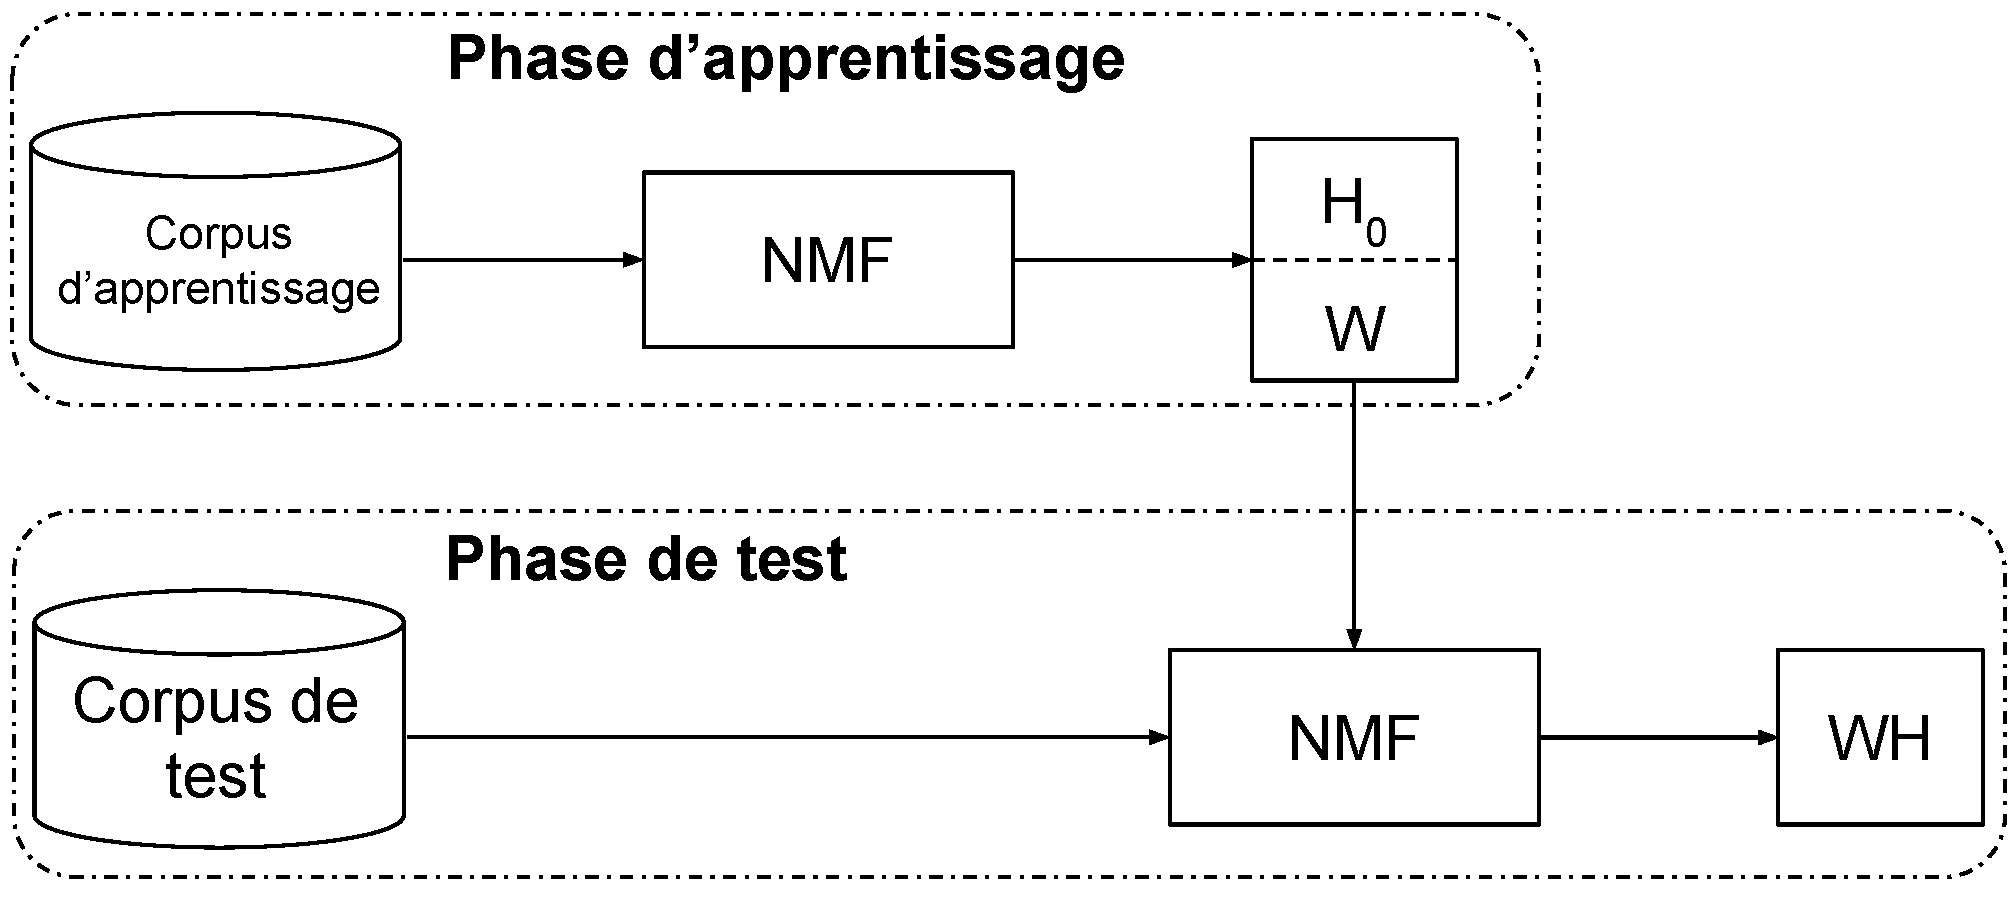
\includegraphics[width=.8\linewidth]{./figures/NMF/NMF_apprentissage.pdf}
\caption{Schéma-bloc des étapes de la NMF.}
\label{fig:supervised_learning}
\end{figure}

\subsection{Apprentissage supervisé et non-supervisé}
Lorsque les classes de sons du corpus d'apprentissage sont inconnues ou que les échantillons audio sont composés d'un mélange de plusieurs sources, il n'est pas possible de connaitre la classe de son de chaque élément qui constitue $\mathbf{W}$. Toutefois, pour réaliser une séparation de sources, il est nécessaire de classifier les différents éléments entre eux. Une étape de \textit{clustering}, à l'aide d'un algorithme des $k$-NN ($k$ plus proche voisins) par exemple, est alors nécessaire pour classer ces éléments selon un nombre de catégories défini par l'utilisateur. Ce cas correspond à une \textit{NMF non-supervisée}.
À l'inverse, lorsque le jeu de données peut être étiqueté, chaque élément défini dans $\mathbf{W}$ est connu. Ce cas, le plus favorable et le plus simple, correspond à une \textit{NMF supervisée}.
En connaissant la classe des éléments de $\mathbf{W}$, la séparation de sources est réalisable. Pour cela, les éléments relatifs à la source d'intérêt $i$ sont extraits soit directement de $\mathbf{W}$ et de $\mathbf{H}$,

\begin{equation}\label{eq:WH_trafic}
\mathbf{\tilde{V}}_i = \left[\mathbf{WH}\right]_i,
\end{equation}

soit cette séparation est réalisée par un filtre de Wiener (ou masquage doux) :

\begin{equation}
\mathbf{\tilde{V}}_i = \frac{\left[\mathbf{WH}\right]_i}{\mathbf{WH}} \otimes \mathbf{V}.
\end{equation}
\\

\subsection{Apprentissage semi-supervisé}
L'apprentissage du dictionnaire pose la question de la généralisation des connaissances : comment à partir de données limitées obtenir une NMF efficace sur un ensemble de cas divers et variés ?  Cette question se base sur le constat qu'il n'est pas possible de modéliser dans $\mathbf{W}$ l'ensemble des classes de sons qui composent un environnement notamment l'ESU qui est un milieu qui inclut une multitude de sources sonores variables. Pour résoudre ce problème, une des premières solutions est de constituer une base d'apprentissage plus importante que la base de test, en vue d'augmenter la généralisation des connaissances apprises ou leur quantité. Toutefois, cette option n'est parfois pas réalisable soit parce que les données ne sont tout simplement pas disponibles, soit parce que la quantité de données à gérer serait ensuite trop importante et nécessiterait des moyens de calculs puissants pour pouvoir mener à bien l'approximation du signal testé.
Une autre possibilité pour tenter de résoudre cette question est de réaliser un apprentissage semi-supervisé, tel que proposé par \cite{lee_semi-supervised_2010, smaragdis2007supervised} (Figure \ref{fig:semi-supervised_learning}). La NMF semi-supervisée propose de construire un dictionnaire $\mathbf{W}_{F \times (K+J)}$ composé d'éléments appris sur le corpus d'apprentissage, $\mathbf{W_s} $ de dimensions $F \times K$, et d'éléments inconnus, $\mathbf{W_r}$ de dimensions $F \times J$ avec $J << K$. Cette condition est nécessaire afin de focaliser la reconstruction du signal avec les sources présentes dans $\mathbf{W_s}$. L'idée est alors de mettre à jour $\mathbf{W_r}$ lors de la phase de test afin d'y intégrer les autres sources sonores qui ne sont pas apprises dans $\mathbf{W_s}$. On obtient donc

\begin{equation}
\mathbf{V} \approx \mathbf{WH} = \mathbf{W_s} \mathbf{H_s} + \mathbf{W_r} \mathbf{H_r}
\end{equation}


avec $\mathbf{W} = \left[ \mathbf{W_s} \mathbf{W_r} \right]$ et respectivement $\mathbf{H} = \left[ \genfrac{}{}{0pt}{0}{\mathbf{H_s}}{\mathbf{H_r}} \right]$ constituée de la matrice $\mathbf{H_s}_{K \times N}$ et de la matrice $\mathbf{H_r}_{J \times N}$. $\mathbf{H_s}$, $\mathbf{W_r}$ et $\mathbf{H_r}$ sont donc les 3 matrices à déterminer lors de la phase de test à l'aide des algorithmes de mises à jour \ref{eq:WH-SSupdate} \cite{kitamura2014music} : 

\begin{figure}[t]
\centering
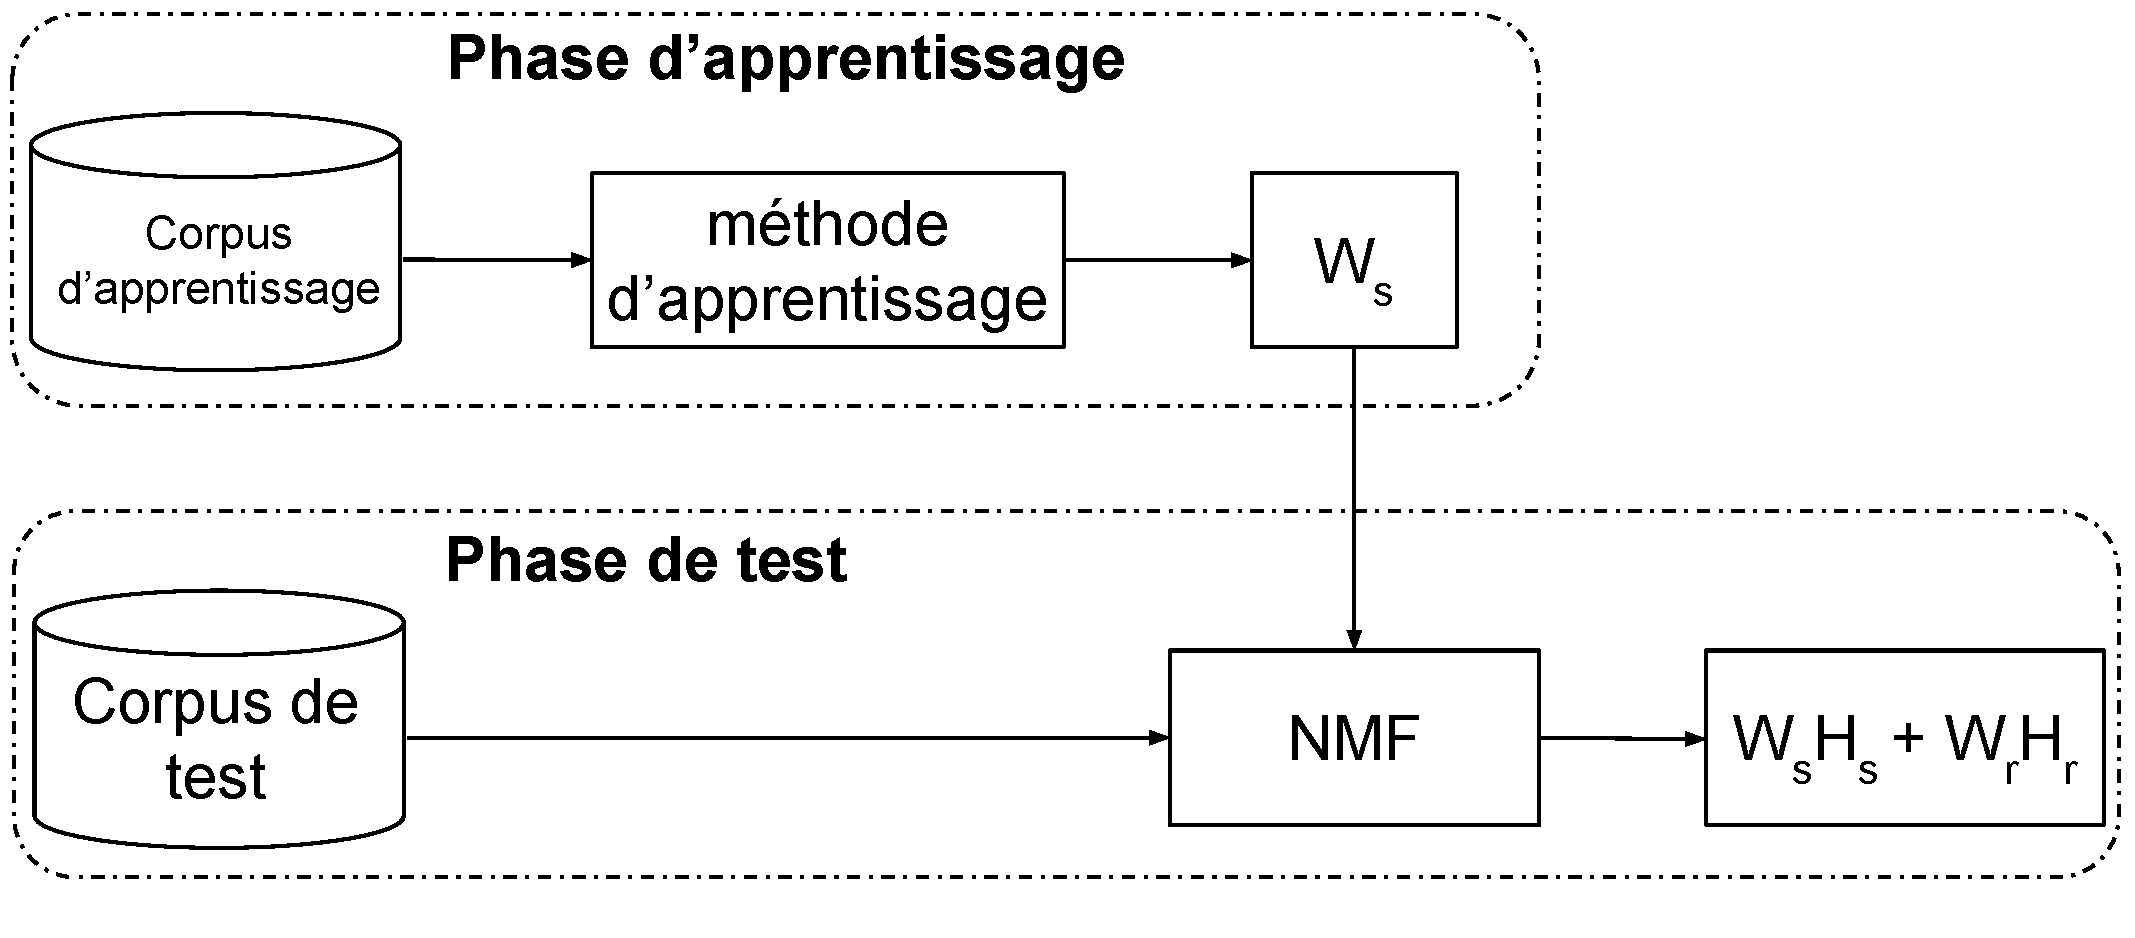
\includegraphics[width=.85\linewidth]{./figures/NMF/NMF_semi-supervised.pdf}
\caption{Schéma-bloc des étapes de la NMF semi-supervisée.}
\label{fig:semi-supervised_learning}
\end{figure}

\begin{subequations}\label{eq:WH-SSupdate}
\begin{align}
\mathbf{W_r}^{(i+1)} &\leftarrow \mathbf{W_r}^{(i)}\otimes\left(\frac{\left[\left(\mathbf{WH}^{(i)} \right)^{.(\beta-2)}\otimes\mathbf{V} \right]\mathbf{H_r}^T}{\left(\mathbf{WH}^{(i)} \right)^{.(\beta-1)}\mathbf{H_r}^T}\right)^{\gamma(\beta)}\label{eq:W_r_SS}\\
\mathbf{H_r}^{(i+1)} &\leftarrow \mathbf{H_r}^{(i)}\otimes\left(\frac{\mathbf{W_r}^T \left[\left(\mathbf{WH}^{(i)} \right)^{.(\beta-2)}\otimes\mathbf{V} \right]}{\mathbf{W_r}^T \left(\mathbf{WH}^{(i)} \right)^{.(\beta-1)}}\right)^{\gamma(\beta)}\label{eq:H_r_SS}\\
\mathbf{H_s}^{(i+1)} &\leftarrow \mathbf{H_s}^{(i)}\otimes\left(\frac{\mathbf{W_s}^T \left[\left(\mathbf{WH}^{(i)} \right)^{.(\beta-2)}\otimes\mathbf{V} \right]}{\mathbf{W_s}^T \left(\mathbf{WH}^{(i)} \right)^{.(\beta-1)}}\right)^{\gamma(\beta)}.\label{eq:H_s_SS}
\end{align}
\end{subequations}

Dans le cas où $\mathbf{W_s}$ est composé de spectres relatifs au trafic, le produit $\mathbf{W_r} \mathbf{H_r}$ est supposé inclure des éléments qui appartiennent à d'autres classes de sons. L'extraction du signal trafic est réalisée à partir de $\mathbf{W_s}$ et de $\mathbf{H_s}$,

\begin{equation}\label{eq:WSHs_trafic}
\mathbf{\tilde{V}}_{trafic} = \mathbf{W_s H_s}
\end{equation}

Plusieurs applications de cette méthode ont été proposées pour des tâches de séparation de sources dans des signaux musicaux \cite{smaragdis2007supervised} ou pour débruiter des signaux contenant de la voix \cite{mysore2011non, duan2012online}). Dans \cite{lefevre2012semi}, une NMF semi-supervisée est réalisée en contraignant la prépondérance des éléments appris dans la reconstruction du signal afin de faciliter l'annotation pour réaliser de la séparation de sources dans des signaux musicaux.


\section{NMF initialisée seuillée}\label{sec:NMF_TI}

Afin de répondre au problème de généralisation de $\mathbf{W}$, une autre approche est proposée : la \textit{NMF initialisée seuillée} (abrégé NMF IS, à ne pas confondre avec la divergence IS qui est la divergence d'Itakura Saïto). Un dictionnaire initial, $\mathbf{W_0}$, est appris sur la source sonore cible (le trafic routier), puis est mis à jour avec $\mathbf{H}$ lors de la phase de test.
Cette technique permet d'orienter les mises à jour de $\mathbf{W_0}$ vers la source d'intérêt et ainsi de considérer les connaissances obtenues \textit{a priori} sur la source tout en adaptant le dictionnaire à la scène sonore testée. Après $N$ itérations, un dictionnaire $\mathbf{W'}$ est obtenu, unique à chaque scène. Pour estimer le signal \textit{trafic}, chaque élément $k$ du dictionnaire, $\mathbf{W'}$, est comparé à son spectre d'origine dans $\mathbf{W_0}$ afin de déterminer s'il est encore assimilable à un spectre \textit{trafic}. La comparaison des 2 éléments est réalisée à travers le calcul de leur similarité cosinus :

\begin{equation}\label{eq:similarite_cosinus}
 D_{\theta}(\mathbf{W_0}\Vert\mathbf{W'}) = \frac{\mathbf{W_0}.\mathbf{W'}}{\Vert\mathbf{W_0}  \Vert. \Vert\mathbf{W'} \vert \vert}
\end{equation}

qui détermine le cosinus de l'angle $\theta$ formé entre les vecteurs $\mathbf{w_0}$ et $\mathbf{w'}$ par le rapport entre leur produit scalaire et leur norme. Dans la suite du document, on se référera à cette distance sous l'abréviation $D_{\theta}$. Cette métrique est invariante d'échelle et est normée entre -1 et 1 :

\begin{itemize}
\item si $D_{\theta} = 1$, les deux vecteurs sont strictement identiques, $\mathbf{w'}$ est alors considéré comme un élément \textit{trafic},
\item si $D_{\theta} = 0$, les deux vecteurs sont orthogonaux, $\mathbf{w'}$ n'est pas une élément \textit{trafic} et est donc rejeté,
\item si $D_{\theta} = -1$, les deux vecteurs sont opposés. Ce cas n'est toutefois pas possible en raison de la contrainte de non-négativité.\\
\end{itemize}

La similarité entre $\mathbf{W_0}$ et $\mathbf{W'}$ correspond alors à une suite de valeurs comprises entre 0 et 1 puis représentées à travers 2 fonctions (Figure \ref{fig:resume_simil}) :

\begin{itemize}
\item une fonction linéaire, $f_{LIN}(k) = D_{\theta}$,
\item une fonction sigmoïde, $f_{SIG}(k) = \sfrac{1}{\left(1+\exp({-\lambda D_{\theta}}\right)}$ avec $\lambda$ le paramètre d'inflexion de la fonction. Cet opérateur réduit la fenêtre de variation de la distance $D_{\theta}$, en diminuant les valeurs élevées et en augmentant les valeurs proches de 0.\\
\end{itemize}

\begin{figure}
    \centering
    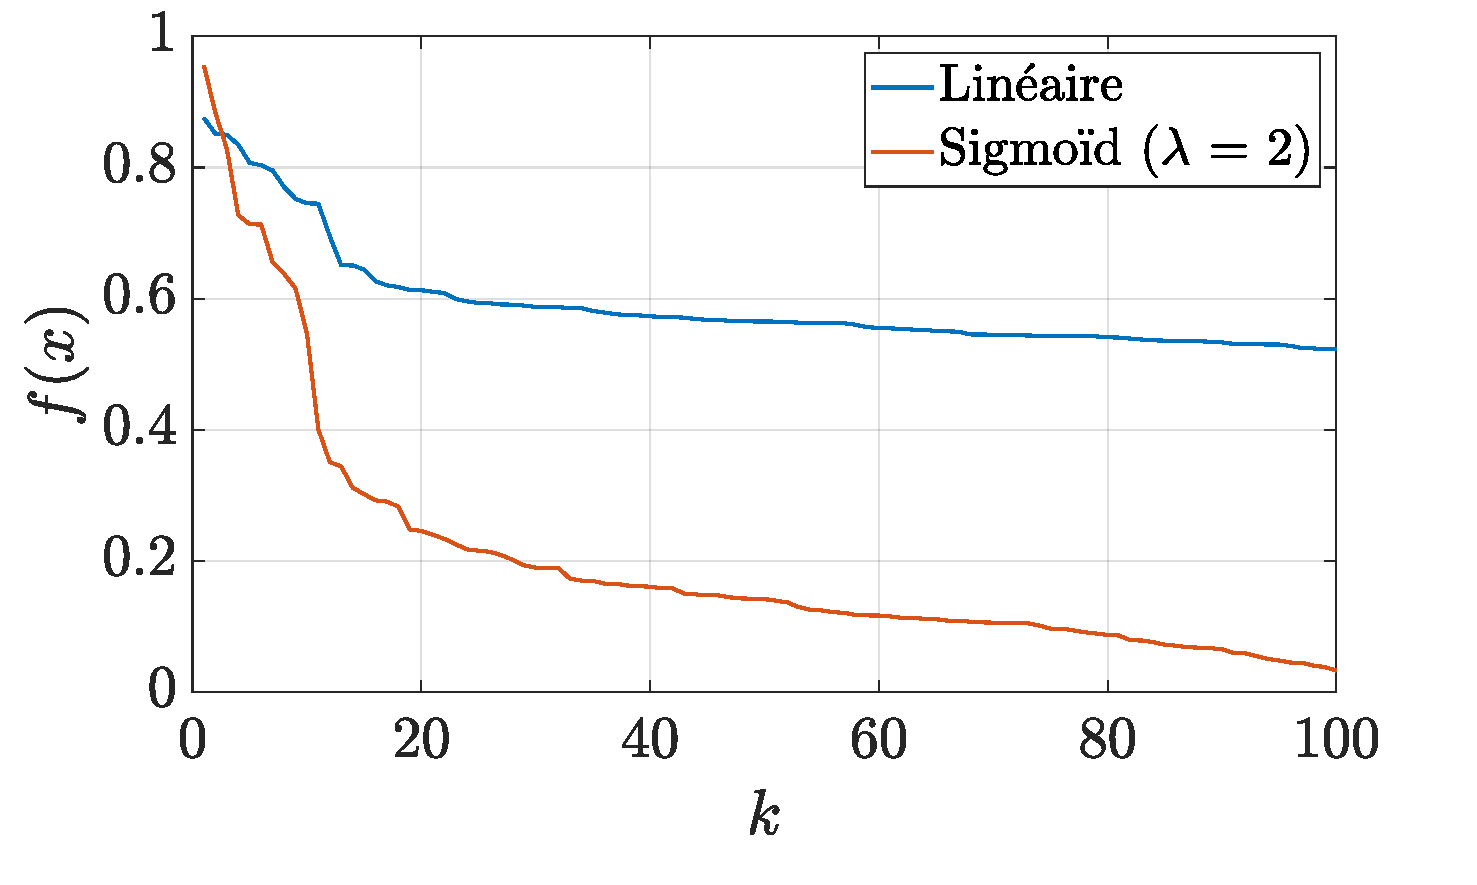
\includegraphics[width=0.7\linewidth]{./figures/NMF/lin_sig.pdf}
    \caption{Similarité cosinus pour une représentation linéaire et sigmoïdienne de la distance $D_{\theta}(\mathbf{W_0} \Vert \mathbf{W'})$ trié dans l'ordre décroissant avec un seuillage dur $t_h$ = 0,6. }
    \label{fig:resume_simil}
\end{figure}

L'extraction du signal \textit{trafic} est réalisée en pondérant alors le produit $\mathbf{W'H}$ tel que

\begin{equation}
\mathbf{\tilde{V}}_{trafic} = \alpha \otimes \left[\mathbf{W'H} \right]
\end{equation}

avec $\alpha = \left[\alpha_1, \alpha_2 \dots \alpha_K \right]$ qui est défini à partir du calcul de similarité (équation \ref{eq:similarite_cosinus}) et d'une méthode de seuillage. 2 méthodes de seuillages sont envisagées :

\begin{itemize}
\item le seuillage dur (\textit{hard thresholding}) \cite{donoho1994threshold} qui consiste à ne considérer dans $\mathbf{W}_{trafic}$ que les éléments de $\mathbf{W'}$ dont la similarité cosinus est supérieure à une valeur seuil $t_h$ :

\begin{subequations}\label{eq:seullageDur_def}
\begin{numcases}{\alpha_k =}
	0 & si \quad $f(k) \leq t_h$,  \\
	1 & si \quad $f(k) > t_h$,
\end{numcases}
\end{subequations}

\item le seuillage \textit{firm} \cite{fornasier2008iterative} qui consiste à pondérer les éléments situés entre deux seuils $t_{f,1}$ et $t_{f,2}$ avec $t_{f,1} < t_{f,2}$, en les normalisant entre 1 et 0 :


\begin{subequations}\label{eq:seuillageFirm_def}
\begin{numcases}{\alpha_k =}
    0, & \text{si}  $f(k) \leq t_{f,1}$, \\
    \Vert f(k)\Vert, & \text{si}  $t_{f,1} < f(k) \leq t_{f,2}$,\\
    1, & \text{si}  $f(k) > t_{f,2}$
\end{numcases}
\end{subequations}
avec $\Vert f(k)\Vert = \frac{f(k)-\min(f(k))}{\max(f(k))-\min(f(k))}$
\end{itemize}

L'allure des pondérations $\alpha$ pour le seuillage dur et \textit{firm} est résumée en Figure \ref{fig:seuillage}.

\begin{figure}
\centering
	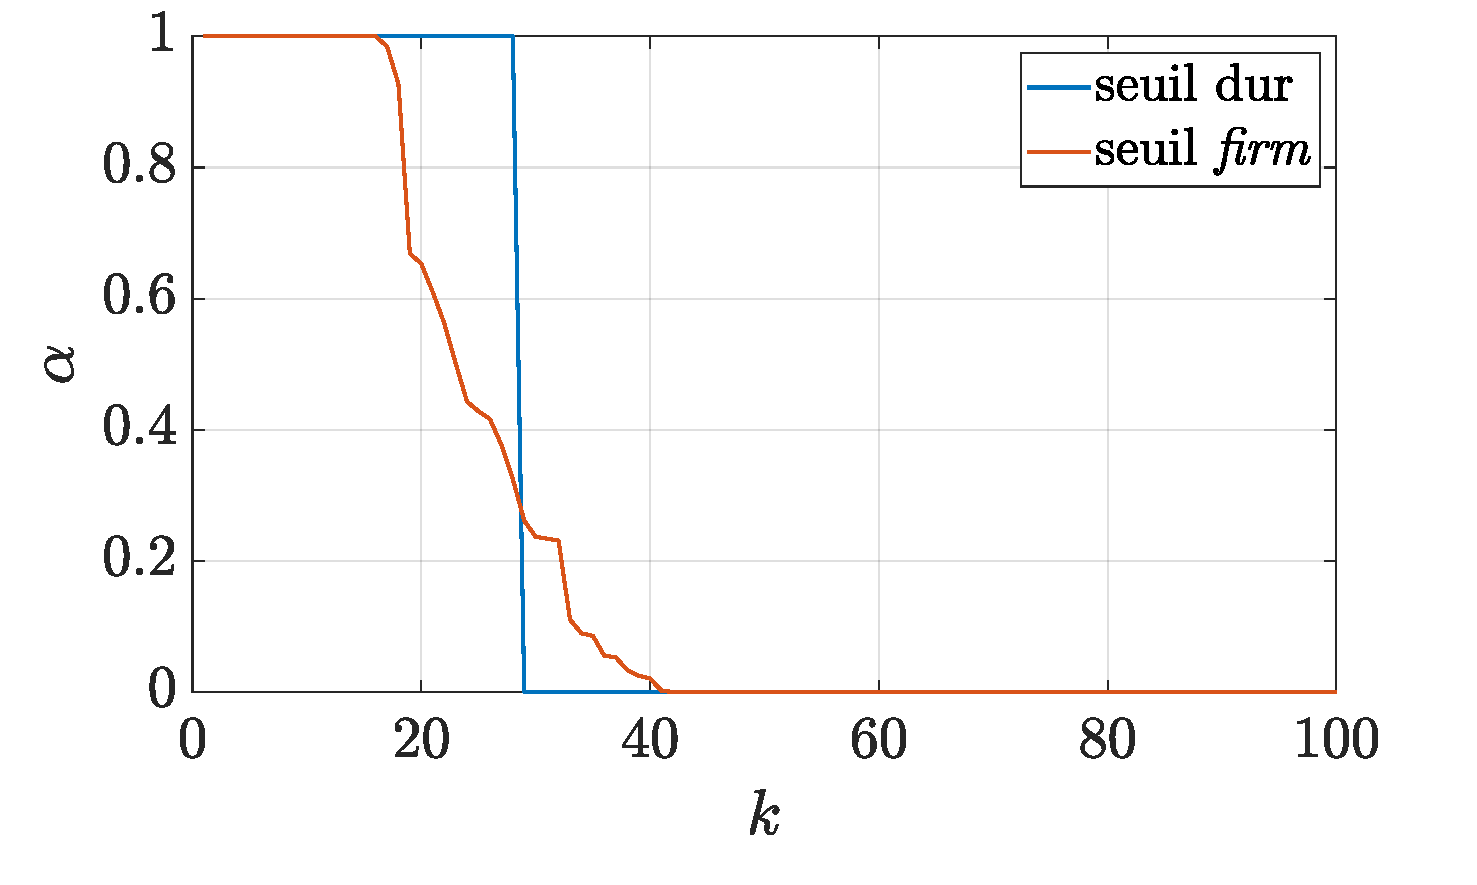
\includegraphics[width=.7\textwidth]{./figures/NMF/seuillage.pdf}
  \caption{Pondération $\alpha$ appliquée à $\mathbf{W'}$, exprimé linéairement, composé de 100 bases avec pour seuil $t_h = 0,2$ (seuillage dur) et $t_{f,1} = 0,15$ et $t_{f,2} = 0,30$ (pour le seuillage \textit{firm}).}
  \label{fig:seuillage}
\end{figure}

On résume les différentes étapes de la NMF IS au travers de l'algorithme \ref{alg:NMF-IS}.

\begin{algorithm}
\caption{NMF initialisée seuillée}
\begin{algorithmic}
\STATE Initialisation de $\mathbf{W_0}$ sur le corpus d'apprentissage
\FOR{i = 1 : nombre itération}
	\STATE mise à jour de $\mathbf{W_0}$
	\STATE mise à jour de $\mathbf{H}$
\ENDFOR
\STATE Calcul de la similarité cosinus $D_{\theta}(\mathbf{W_0} \Vert \mathbf{W'})$
\IF{représentation sigmoïde}
	\STATE $D_{\theta}(\mathbf{W_0} \Vert \mathbf{W'}) = \sfrac{1}{\left(1+\exp({-\lambda D_{\theta}(\mathbf{W_0} \Vert \mathbf{W'})}\right)}$
\ENDIF

\IF{seuillage \textit{dur}}
	\STATE $\alpha$ définit selon Eq. \ref{eq:seullageDur_def}
\ELSIF{seuillage \textit{firm}}
	\STATE $\alpha$ définit selon Eq. \ref{eq:seuillageFirm_def}
\ENDIF
\STATE $\mathbf{\tilde{V}}_{trafic} = \alpha \mathbf{W'H}$
\end{algorithmic}
\label{alg:NMF-IS}
\end{algorithm}

L'intérêt de cette approche est qu'elle permet, par la mise à jour du dictionnaire $\mathbf{W_0}$ de modéliser directement la source sonore \textit{trafic} avec les effets de l'environnement sur la propagation sonore. En effet, la NMF supervisée et semi-supervisée possède un dictionnaire fixe (ou dans une grande partie fixe pour la semi-supervisée) avec lequel elles doivent modéliser l'ensemble de cette source. Par rapport au problème posé dans la partie \ref{part:problème}, elles  contiennent dans $\mathbf{W}$, la source $\hat{s}_{v_j}(f)$. La NMF IS, en calculant $\mathbf{W'}$, contient dans son dictionnaire l'ensemble des sources présentes filtrées par l'environnement urbain. L'extraction du signal \textit{trafic} de $\mathbf{W'H}$ permet alors de déterminer $\hat{S}_{tr.}(f)$, ce qui permet une plus grande généralisation de la méthode. Toutefois, en mettant à jour la forme de chaque élément, on perd la supervision du dictionnaire puisque certains spectres de $\mathbf{W_0}$ appartenant initialement à la source \textit{trafic} peuvent être déviés en une autre source. La méthode de seuillage pour déterminer les composantes \textit{trafic} permet de conserver les éléments qui dévient le moins. Mais cette technique génère un risque de considérer des éléments de la classe \textit{interférante} si le seuil $t_h$ (ou $t_{f,1/2}$) est trop faible ou bien pas assez d'éléments si il est trop élevé.

\section{NMF avec contraintes}\label{part:NMF_contrainte}
Les différentes variantes de la NMF présentées ne sont soumises, jusqu'ici, qu'à la contrainte de non-négativité avec pour objectif la minimisation de l'équation \ref{eq:D(V-WH)}. Toutefois, l'ajout de contraintes sur l'apprentissage du dictionnaire ou sur l'allure de la matrice d'activation est possible suivant les connaissances que l'on a \textit{a priori} de ces éléments. Ces contraintes sont alors prises en compte dans la fonction de coût \ref{eq:D(V-WH)} par l'ajout d'un second terme pondéré $C(\mathbf{W},\mathbf{H})$. Le problème devient alors :

\begin{equation}\label{eq:costFunctionPenalized}
\text{min}~D\left(\textbf{V} \Vert \textbf{WH}\right) + \alpha C(\mathbf{W},\mathbf{H}) \quad \text{avec} \quad \mathbf{W} \geq 0, \mathbf{H} \geq 0.
\end{equation}

Si l'allure de $\mathbf{W}$ ou $\mathbf{H}$ n'est pas celle souhaitée, la fonction de coût \ref{eq:costFunctionPenalized} augmente. Les algorithmes de mise à jour vont alors considérer cette contrainte afin de favoriser les matrices qui permettent de minimiser au mieux cette fonction de coût. Le terme de pondération $\alpha$ permet de faire varier le poids de la contrainte : plus ce terme est grand et plus son influence sera prépondérante. Plusieurs types de contraintes sont décrites et serviront dans la suite de l'étude.

\subsection{Contrainte de parcimonie}\label{part:sparsness}
Une des premières contraintes employées est celle de la parcimonie \cite{hoyer_non-negative_2004, le2015sparse} : c'est-à-dire l'utilisation d'un nombre réduit d'éléments du dictionnaire à chaque instant $t$. Cette contrainte renforce la représentation par partie de la NMF en pénalisant les termes qui seraient non nuls. Elle trouve notamment son intérêt dans le cas d'une représentation \textit{sur-complète} du dictionnaire, c'est à dire $K > \max(F,N)$ où l'ajout de la contrainte parcimonieuse permet de réduire la complexité du problème \cite{eggert2004sparse}. Dans un premier temps, Hoyer \cite{hoyer_non-negative_2004} propose une contrainte telle que

\begin{equation}
C(h_k) = \frac{\sqrt{N}-\left( \sum_{n=1}^N \vert h_{kn} \vert \/ \sqrt{\sum_{n = 1}^N h_{kn}^2} \right)}{\sqrt{N}-1}
\end{equation}

qui équivaut au rapport de la norme $\ell_1$ et $\ell_2$ normalisée de $h_{kn}$. Ce rapport est ensuite défini tel que $C(h_k) = C_h$, une valeur constante définie qui fixe la quantité de parcimonie souhaitée dans $\mathbf{H}$. Un algorithme de gradient de descente permet ensuite, sous cette contrainte, de résoudre l'équation \ref{eq:D(V-WH)}. Virtanen \cite{virtanen_monaural_2007} propose l'ajout d'une contrainte $C_{sp}(\mathbf{h})$, le plus souvent considérée comme la norme $\ell_1$ des éléments de $\mathbf{H}$,

\begin{equation}\label{eq:sparsness}
C_{sp}(\mathbf{h}) = \sum_k h_{kn}.
\end{equation}

Cette pénalisation peut facilement être prise en compte dans les algorithmes de \textit{majorisation-minimisation} :

\begin{equation}
\underset{\textbf{h > 0}}{\text{min}}~C(\mathbf{h}) = D(\mathbf{v} \vert\vert \mathbf{Wh}) + \alpha_{sp} C_{sp}(\mathbf{h})
\end{equation}

avec $\alpha_{sp}$, la pondération respective à la contrainte de parcimonie. La fonction auxiliaire pénalisée $G_p(\mathbf{h}^{(i+1)}\vert \mathbf{h}^{(i)})$ devient alors

\begin{equation}
G_p(\mathbf{h}^{(i+1)}\vert \mathbf{h}^{(i)}) = G(\mathbf{h}^{(i+1)}\vert \mathbf{h}^{(i)})+ \alpha_{sp}C_{sp}(\mathbf{h}^{(i+1)})
\end{equation}

et a pour dérivée selon $h_k$

\begin{equation}\label{eq:derivé-fonc-auxiliaireSparse}
\nabla_{h_k} G_p(\mathbf{h}^{(i+1)}\vert \mathbf{h}^{(i)}) = \sum_f w_{fk}\left[\breve{d}'\left(v_f\vert v_f^{(i)}\frac{h_k^{(i+1)}}{h_k^{(i)}}\right) + \textit{\textroundcap{d}}'(v_f\vert v_f^{(i)})\right]+\alpha_{sp}.
\end{equation}

L'algorithme de mise à jour de $\mathbf{H}$ devient alors

\begin{subequations}\label{eq:h_sparsity}
\begin{numcases}{\textbf{H}^{(i+1)} \leftarrow}
  \textbf{H}^{(i)} \otimes\left(\frac{\textbf{W}^T \left[\left(\textbf{WH}^{(i)} \right)^{(\beta-2)} \otimes \textbf{V} \right]}{\textbf{W}^T \left[\textbf{WH}^{(i)} \right]^{(\beta-1)}+ \alpha_{sp}}\right)^{\gamma(\beta)} & $\beta < 2$,\label{eq:h_sparsity_1}\\
    \textbf{H}^{(i)} \otimes\left(\frac{\textbf{W}^T \left[\left(\textbf{WH}^{(i)} \right)^{(\beta-2)} \otimes \textbf{V} \right]-\alpha_{sp}}{\textbf{W}^T \left[\textbf{WH}^{(i)} \right]^{(\beta-1)}}\right)^{\gamma(\beta)}, & $\beta \geq 2$.\label{eq:h_sparsity_2}
\end{numcases}
\end{subequations}

Dans le cas où $\beta \geq 2$, la contrainte apparait au numérateur et est soustractive. Ce comportement peut être problématique dans le cadre de la non-négativité suivant la value de $\alpha_{sp}$ \cite{fevotte_algorithms_2011}. En Figure \ref{fig:sparsity_example}, un exemple de l'effet de la parcimonie sur l'allure d'un élément $j$ de la matrice $\mathbf{H}$ pour 3 valeurs de parcimonie. Avec l'augmentation de la valeur de la pondération, certaines activations présentes lorsque la contrainte est absente, mais de faibles amplitudes, deviennent nulles. 

\begin{figure}[h]
\centering
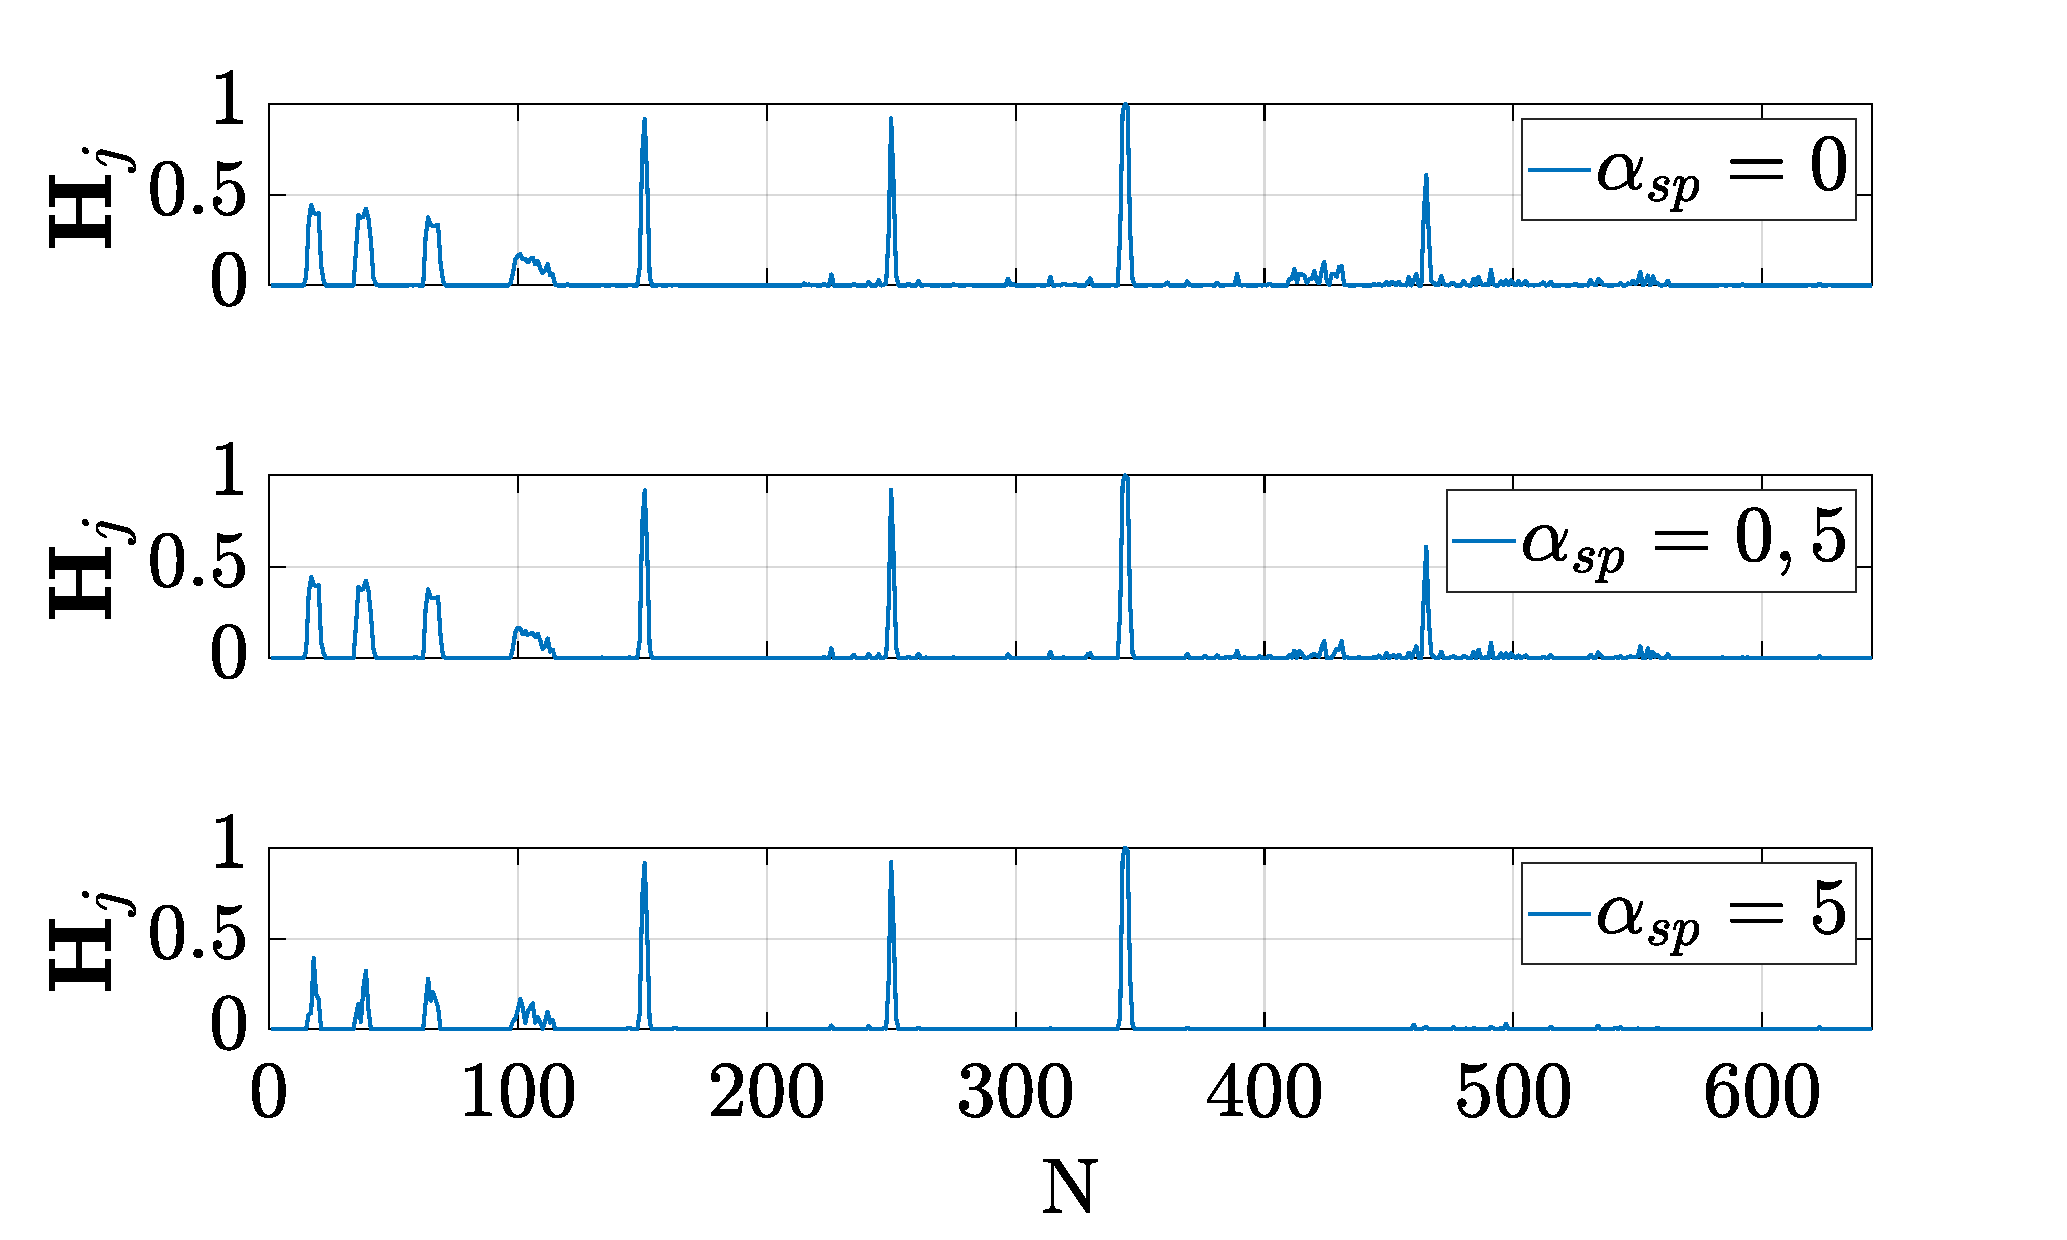
\includegraphics[width=.8\linewidth]{./figures/resultats/sparsity_example.pdf}
\caption{Exemple de l'effet de la parcimonie pour une scène du corpus \textit{alerte} pour $\alpha_{sp} \in \lbrace
0,~0,5,~5\rbrace$.}
\label{fig:sparsity_example}
\end{figure}


\subsection{Contrainte de régularité temporelle}\label{part:smoothness}

La mise à jour de la matrice d'activation $\mathbf{H}$ se fait par défaut trame par trame sans considérer de liens entre les trames $n$ et les précédentes. Néanmoins, la plupart des sons réels ont une évolution temporelle lente. Prendre en compte l'évolution des trames temporelles adjacentes peut permettre que la forme des activateurs soit plus réaliste et que l'outil soit plus robuste dans la reconstruction du signal. Cette contrainte trouve son intérêt dans la musique (\cite{virtanen_sound_2003, fevotte_majorization-minimization_2011}) où les instruments (à l'exception des instruments percussifs) peuvent jouer des notes durant, au moins, plusieurs centaines de milli-secondes. Mais c'est aussi le cas au sein d'environnements sonores urbains où les sons (notamment le trafic routier) ont des variations lentes, de plusieurs secondes. L'une des approches les plus citées est celle de Virtanen \cite{virtanen_monaural_2007}, qui fut ensuite généralisée sous la forme d'un algorithme générique dans \cite{fevotte2017single}, avec l'ajout d'une contrainte $C_t(\mathbf{H})$ :

\begin{equation}\label{eq:smoothnessVirtanen}
C_t(\mathbf{H}) = \sum_{n=1}^K \sum_{n=2}^N \left(h_{kn} - h_{k(n-1)}\right)^2.
\end{equation}

La pondération de cette contrainte peut être constante sur tous les éléments ($\alpha_t$) ou bien être variable selon $k$ ($\alpha_{t,k})$ et doit donc être placée dans la somme. Par l'ajout de cette contrainte, les fortes variations d'un vecteur d'activation entre l'indice $n$ et $n-1$ sont pénalisées par la mise au \textit{carré} de leur distance. La mise à jour de $\mathbf{H}$ privilégie alors les variations plus lentes pour réduire le poids de la contrainte $C_t(\mathbf{H})$. L'algorithme de mise à jour devient :

\begin{equation}
\textbf{H}^{(i+1)} \leftarrow \textbf{H}^{(i)} \otimes\left(\frac{\textbf{W}^T \left[\left(\textbf{WH}^{(i)} \right)^{(\beta-2)} \otimes \textbf{V} \right] + 2 A \otimes \left(\overrightarrow{\mathbf{H}}^{(i)} + \overleftarrow{\mathbf{H}}^{(i)} \right)}{\textbf{W}^T \left[\textbf{WH}^{(i)} \right]^{(\beta-1)} + 2 A \otimes \left(\mathbf{H}^{(i)} + \overleftrightarrow{\mathbf{H}}^{(i)} \right)}\right)^{\gamma(\beta)}\label{eq:HupdateSmooth}
\end{equation}

avec

\begin{subequations}
\begin{align}
    A &=
\begin{bmatrix}
\alpha_{t,1} &  \cdots & \alpha_{t,1}  \\
\alpha_{t,2} & \dots & \alpha_{t,2}  \\
\vdots & \ddots &  \vdots \\
\alpha_{t,K} & \cdots & \alpha_{t,K}
\end{bmatrix}, \label{eq:subeq1}\\
    \overrightarrow{\mathbf{H}} &=
\begin{bmatrix}
0 & h_{1,1} & h_{1,2} & \cdots & h_{1,N-1}\\
0 & h_{2,1} & h_{2,2} & \cdots & h_{2,N-1}\\
\vdots & \vdots & \vdots & \ddots & \vdots\\
0 & h_{K,1} & h_{K,2} & \cdots & h_{K,N-1}\\
\end{bmatrix}, \label{eq:subeq2}\\
    \overleftarrow{\mathbf{H}} &=
\begin{bmatrix}
h_{1,2} & h_{1,3} & \cdots & h_{1,N} & 0\\
h_{2,2} & h_{2,3} & \cdots & h_{2,N} & 0\\
\vdots & \vdots & \ddots & \vdots & \vdots\\
h_{K,2} & h_{K,3} & \cdots & h_{K,N} & 0\\
\end{bmatrix}, \label{eq:subeq3}\\
    \overleftrightarrow{\mathbf{H}} &=
\begin{bmatrix}
0 & h_{1,2} & \cdots & h_{1,N-1} & 0\\
0 & h_{2,2} & \cdots & h_{2,N-1} & 0\\
\vdots & \vdots & \ddots & \vdots & \vdots\\
0 & h_{K,2} & \cdots & h_{K,N-1} & 0\\
\end{bmatrix}. \label{eq:subeq5}
\end{align}
\end{subequations}

$A$ résume les valeurs des contraintes selon $k$, $\overrightarrow{\mathbf{H}}$, les valeurs de $\mathbf{H}$ à l'instant $n-1$, $\overleftarrow{\mathbf{H}}$, les valeurs de $\mathbf{H}$ à l'instant $n+1$ et enfin $\overleftrightarrow{\mathbf{H}}$, les valeurs de $\mathbf{H}$ sur l'intervalle $\left[2,N-1 \right]$. L'impact du coefficient de pondération $\alpha_t$ sur les activations de $\mathbf{H}$ est représenté en Figure \ref{fig:smoothnessExample}. Plus cette pondération est forte plus l'allure des activateurs est régulière. C'est cet algorithme qui a été implémenté et testé pour les travaux de cette thèse.

\begin{figure}[hbtp]
\centering
	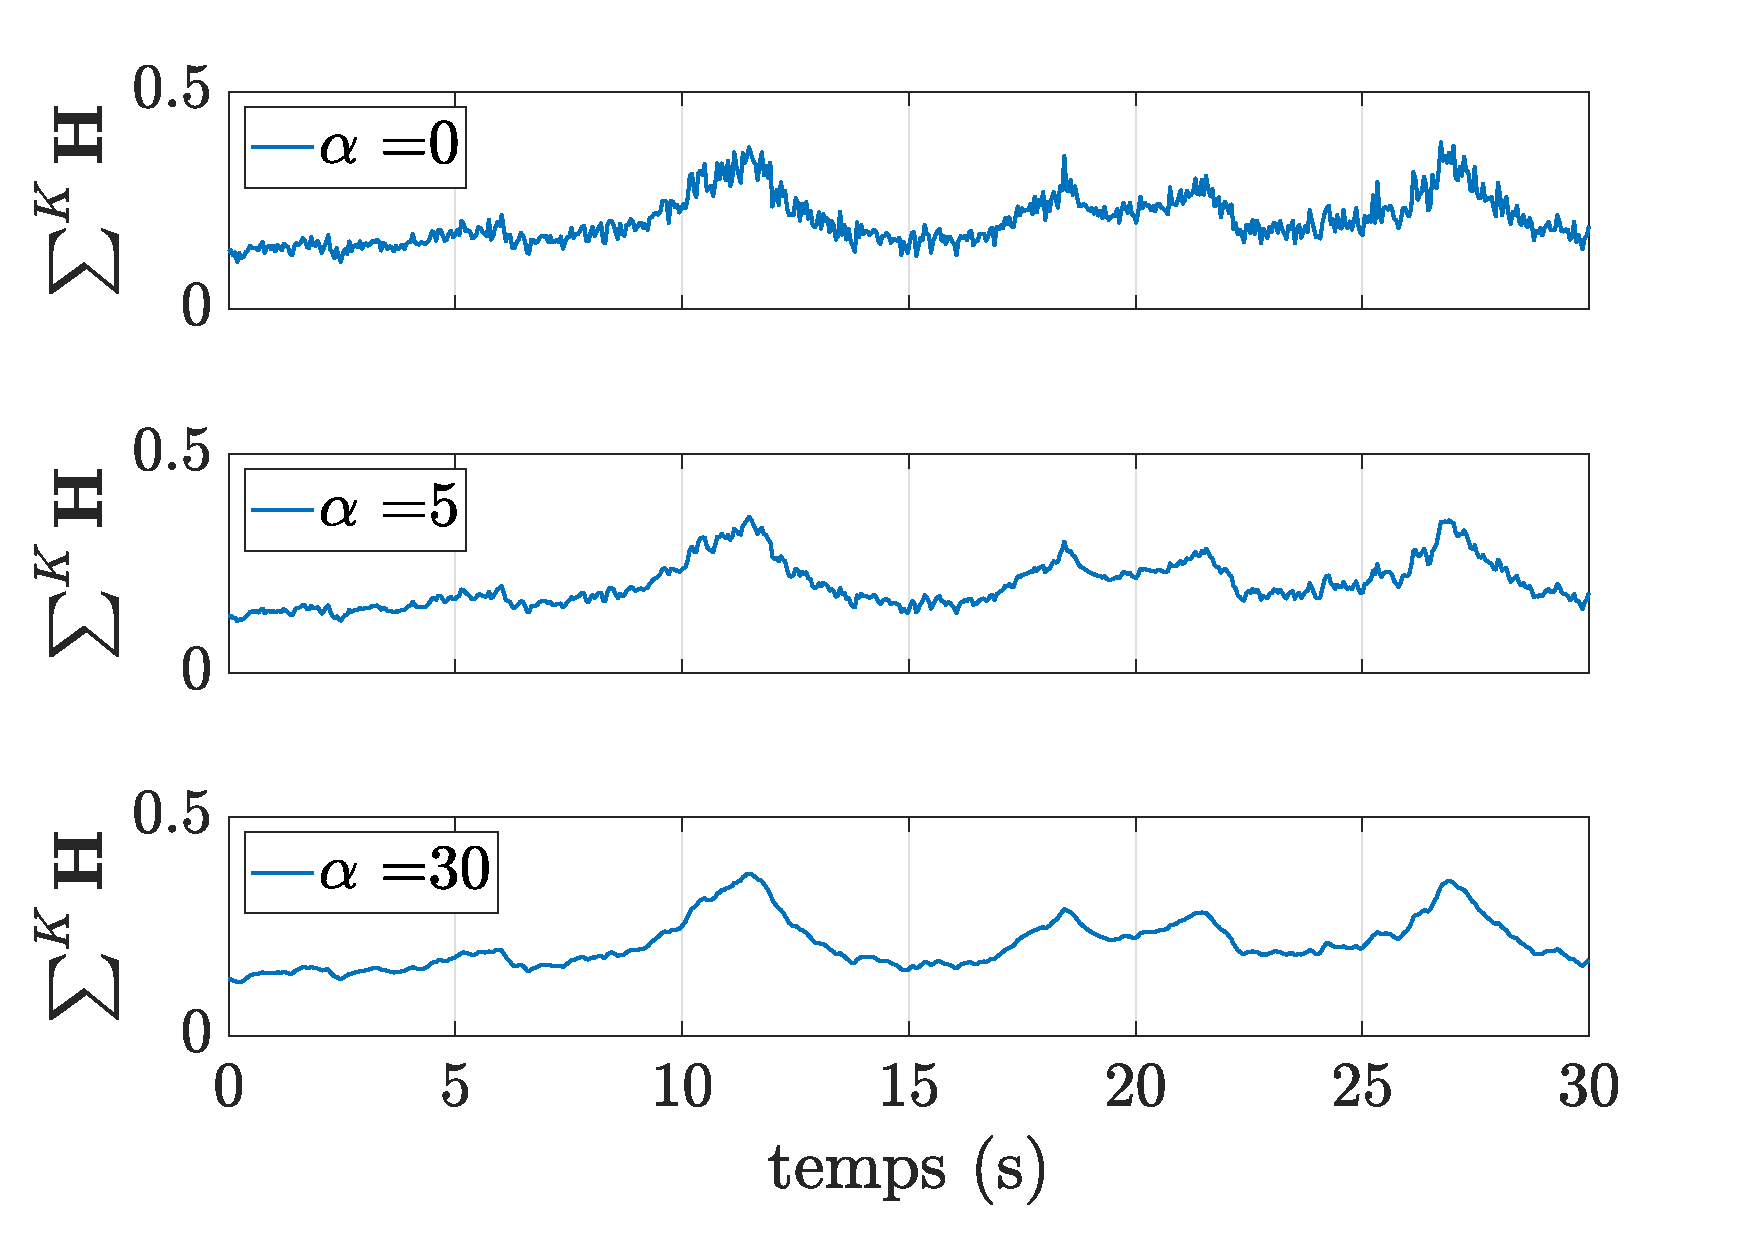
\includegraphics[width=0.7\linewidth]{./figures/NMF/smoothness_02.pdf}
\caption{Influence de la pondération $\alpha$ de la contrainte temporelle $C_t(\mathbf{H})$ sur la somme; selon $K$, des activateurs sur une scène audio de 30 secondes.}
\label{fig:smoothnessExample}
\end{figure}

D'autre approches ont également été étudiées. Dans, \cite{fevotte2011majorization}, dans le cas de la séparation de sources audio et la transcription d'un morceau de musique, une contrainte de régularité est proposée pour la divergence I-S. La particularité de la contrainte apposée est qu'elle se base elle-même sur la divergence I-S : $C_{I-S}(\mathbf{H}) = \sum_{k = 1}^{K} \sum_{n = 2}^{N}d_0(h_{k(n-1)} \vert h_{kn})$. L'algorithme de mise à jour est déduit à partir de l'algorithme de \textit{majorisation-minimisation} (voir partie \ref{part:majorisation-minimisation}). Dans \cite{essid2013smooth}, une contrainte, similaire à l'équation \ref{eq:smoothnessVirtanen} ($C_{MM}(\mathbf{H}) = \frac{1}{2}\sum_{k = 1}^{K} \sum_{n = 2}^{N}\left(h_{kn}-h_{k(n-1)}\right)^2$), est proposée dans le cas de la structuration de documents audiovisuels pour une divergence K-L avec, là encore, l'utilisation d'un algorithme de \textit{majorisation-minimisation}. Cette approche a été développée durant la thèse pour la divergence I-S et la distance EUC mais n'a pas été utilisée pour ces travaux. Les détails des calculs se situent en annexe \ref{annex:smoothNMF}.
Enfin on peut citer \cite{pascual2006nonsmooth} où une contrainte de \og non-smoothness \fg{} est considérée. L'idée est alors d'imposer de l'adoucissement dans la NMF sur une des deux matrices pour générer, en réaction inverse, de la parcimonie dans l'autre matrice. Le problème est ainsi posé :

\begin{equation}
\mathbf{V} \approx \mathbf{WSH}
\end{equation}

où $\mathbf{S}$ est une matrice de \textit{smoothness} telle que

\begin{equation}
\mathbf{S} = (1-\alpha_t)\mathbf{I}+\frac{\alpha}{K}\mathbf{11}^T
\end{equation}

avec $\mathbf{I}$ la matrice identité, $\mathbf{1}$ un vecteur unitaire et $\alpha_t$ un paramètre de \textit{smoothness} compris entre 0 et 1. Lorsque $\alpha = 0$, la régularité temporelle est nulle alors que pour $\alpha_t = 1$, le produit $\mathbf{SH}$ (ou $\mathbf{WS}$) génère un vecteur constant qui correspond à la moyenne des éléments de $\mathbf{H}$ (ou $\mathbf{W}$). Ce cas présente alors une parcimonie nulle puisque toute les entrées sont égales et non-nulles (là où une plus forte parcimonie présente des valeurs proches de 0).

\subsection{Autres contraintes}

D'autres contraintes existent dans la littérature mais ne seront pas étudiées dans ces travaux.
On peut citer une contrainte sur l'\textbf{harmonicité} des éléments de $\mathbf{W}$ qui a été proposée dans \cite{vincent2008harmonic} dans le cadre de la transcription d'une mélodie de piano. Le dictionnaire est alors décomposé en une somme de partiels sinusoïdes harmoniques ou inharmoniques pondérées selon une enveloppe spectrale. \cite{rigaud2012piano} propose une autre approche où une contrainte d'inharmonicité est imposée permettant à chaque élément de $\mathbf{W}$ de modifier la fréquence de chaque partiel tout en contraignant l'ensemble à suivre une loi d'inharmonicité.

La \textbf{NMF locale} a été proposée par \cite{li2001learning} qui contraint la fonction de coût avec trois pénalités : i) le nombre de bases $K$ doit être minimisé, ii) les bases doivent être le plus orthogonales que possible, iii) seules les bases qui donnent le plus d'informations sont conservées. Son application à la classification d'instruments de musique dans \cite{benetos2006musical} est toutefois peu efficace.

Dans le cadre de la NMF semi-supervisée, une contrainte est proposée dans \cite{yagi2012music}, puis étendue dans \cite{kitamura2014music} pour toute valeur de $\beta$, dans le cadre de la séparation de signaux musicaux afin de \textbf{maximiser la distance} (ou la divergence) entre le dictionnaire appris $\mathbf{W_s}$ et le dictionnaire libre $\mathbf{W_r}$ afin de s'assurer qu'un minimum d'information d'intérêt y soit intégré. Dans \cite{wang2016semi}, c'est une contrainte de propagation qui est considérée où un nouveau dictionnaire $\mathbf{W}$ est construit dans lequel les éléments similaires dans $\mathbf{W_r}$ à ceux appris et étiquetés sont pondérés. Dans \cite{lefevre2012semi}, la contrainte ajoutée consiste à pondérer le poids des éléments appris dans la reconstruction de $\mathbf{V}$ afin de donner une prépondérance différente des éléments non-appris.\\

\section{Conlusion du chapitre}

La Factorisation en Matrices Non-négative est une méthode qui permet l'approximation d'un spectrogramme en amplitude (ou en puissance) d'un enregistrement audio par le produit de deux matrices : $\mathbf{W}$, le dictionnaire composé de spectres sonores, et $\mathbf{H}$, la matrice d'activation. Différentes formes de NMF ont été proposées qui diffèrent selon les techniques d'apprentissage de leur dictionnaire (non-supervisée, supervisée et semi-supervisée) ou des contraintes qui y sont appliquées (parcimonie, régularité temporelle). Plusieurs de ces NMF sont implémentées dans le cas de ces travaux et testées en vue de déduire, sur des corpus de sons présentés dans le chapitre suivant, le niveau sonore du trafic routier.
La \textbf{NMF supervisée}, \textbf{semi-supervisée} et, celle proposée, \textbf{initialisée seuillée} sont les trois approches retenues. L'influence de la contrainte de \textbf{régularité temporelle} $C_t(\mathbf{H})$  est  également observée pour un des corpus de sons dans le chapitre \ref{chap:grafic}. Les 3 $\beta$-divergences détaillées (\textbf{distance EUC} ($\beta = 2$), \textbf{divergence K-L} ($\beta = 1$) et \textbf{I-S} ($\beta = 0$)) seront celles utilisées sur chaque corpus.


%%%%%%%%%%%%%%%%%%%%%%%%%%%%%%%%%%%%%%%%%%%%%%%%%%%
%\bibliographystyle{unsrt}
%\bibliography{../bibliographie}
%
%\end{document}
%\documentclass[twoside,openright,a4paper,11pt]{book}
%
%
\usepackage[utf8]{inputenc}
\usepackage[francais]{babel}
\usepackage[T1]{fontenc}

\addto\captionsfrench{\def\tablename{\textsc{Tableau}}}% pour avoir TABLEAU et pas TABLE dans les légendes des tableaux

%%%%%%% MISE EN PAGES %%%%%%
\usepackage{geometry}
\geometry{outer=2cm,inner=3cm,top=3cm}

\setcounter{tocdepth}{3}     % Dans la table des matieres
\setcounter{secnumdepth}{3}  % Avec un numero.
\usepackage{setspace}

\usepackage{fancyhdr}	% marge en haut et en bas
\pagestyle{fancy}

\fancyhead{}	% vide l'entête
\fancyfoot{} % vide le pied~de~page

\fancyhead[RO]{\leftmark}
\fancyhead[LE]{\rightmark}
\fancyfoot[C]{\thepage}	% numéro de page en bas au centre

\renewcommand{\headrulewidth}{0.4pt} % épaisseur du trait en haut
\renewcommand{\footrulewidth}{0.4pt} % épaisseur du trait en bas

\fancypagestyle{mypagestyle}{%
    \fancyhead{}	
    \fancyfoot{} 
    \fancyfoot[C]{\thepage}
    \renewcommand{\headrulewidth}{0.4pt} 
	\renewcommand{\footrulewidth}{0.4pt} 
}

\fancypagestyle{couvertureAbstract}{%
    \fancyhead{}	
    \fancyfoot{} 
    \fancyfoot[C]{}
	\renewcommand{\headrulewidth}{0pt} 
	\renewcommand{\footrulewidth}{0pt} 
}
%
\usepackage{layout}
\usepackage{tocbibind} % include tableofcontent in itself

%%%%%% PAGE DE GARDE %%%%%%

\geometry{outer=2cm,inner=3cm,top=3cm}
\usepackage[scaled]{helvet} % font used on cover (Helvetica)
\usepackage{eso-pic} % to set background picture
\usepackage{multicol} % for back cover (abstracts)
\usepackage{graphicx} % to include logos
\usepackage{tikz} % to compose background picture

% Colors (extracted from SPI's template)
\definecolor{boxcolor1}{rgb}{0.91373,0.92941,0.87451}
\definecolor{boxcolor2}{rgb}{0.94902,0.93333,0.91373}
\definecolor{boxcolor3}{rgb}{0.76078,0.87843,0.17647}
\definecolor{headercolor}{rgb}{0.94118,0.30980,0.17255}
\definecolor{namecolor}{rgb}{1.0,0.4,0.0}
\definecolor{titlecolor}{rgb}{0.19216,0.51765,0.60784}
% Also used: gray, teal (predefined by xcolor package, usually loaded by document class)

% Cover environment, to keep changes local
\newenvironment{cover}{%
  \fontfamily{phv}\selectfont % Select Helvetica font
  \pagestyle{empty} % No page number
}{
  \addtocounter{page}{-1}
  \cleardoublepage
}

% Macro for background common to front and back
\newcommand{\tikzBG}{%
  \path (0,0) rectangle (1,1);
  %TODO: You should adjust the bottom height of the following rectangle to fit your abstract's length
  \path [fill=boxcolor1] (.0571,.11) rectangle (.481,.963); 
  \path [fill=boxcolor2] (.4333,.697) rectangle (.9048,.7475);
  \path [fill=boxcolor2] (.4333,.7811) rectangle (.9048,.8316);
  \path [fill=boxcolor2] (.4333,.8687) rectangle (.9048,.9192);
  \path [fill=boxcolor3] (.0571,.7879) rectangle (.5762,.8316);
  \node[inner sep=0pt] at (0.2285,0.8788) [above left] {%
    
\includegraphics[height=.0707\paperheight,keepaspectratio]{./figures/logo/logo_unb.png}};
  \node[inner sep=0pt] at (0.6667,0.8788) [above right] {%
    
\includegraphics[height=.0808\paperheight,keepaspectratio]{./figures/logo/logo_ecn_color.png}};
  \node at (.0571,.8316) [above right,color=headercolor] {%
    \fontsize{29}{35}\selectfont\bfseries Th\`ese de Doctorat};
}

% Macro for repeated information (to avoid insconsistency)
%TODO: fill in with no formatting but desired case
\newcommand{\firstName}{Jean-Rémy}
\newcommand{\surname}{Gloaguen}
\newcommand{\thesisTitle}{Estimation du niveau sonore de sources d'intérêts au sein de mixtures sonores urbaines : application au trafic routier}

%%%%%%% SYMBOLES %%%%%
\usepackage{tipa}	% pour avoir l'accent concave
\usepackage{lmodern}	% pour les guillemets
\usepackage{gensymb}	% pour les degrés
\usepackage{enumitem}	% pour changer le symbole de l'item (\begin{itemize}[label=$\bullet$])

%%%%%%% EQUATION %%%%%%
\usepackage{amssymb}
\usepackage{amsmath}
\usepackage{fancybox}
\usepackage{xfrac}	% fraction de type "1/4"
\usepackage{cases}	% système équation
\usepackage[overload]{empheq}
\usepackage{bm}		% pour mettre en gras .
\usepackage{units} 	% x/y barre latérale pour les fractions
%
%%%%%%% FIGURE %%%%%%
\usepackage{subfigure}	% utiliser subfigure
\usepackage{float}	% utiliser H dans les figures
%
%%%%%% TABLEAUX %%%%%%
\usepackage{array,multirow,makecell}
%\addto\captionsfrench{\def\tablename{\textsc{Tableau}}}% pour avoir TABLEAU et pas TABLE dans les légendes des tableaux
\usepackage{colortbl} % pour avoir des lignes colorées dans les tableau
%\usepackage{slashbox} % pour les \backslashbox
%\usepackage{subcaption}
\usepackage{hhline}	% pour les lignes horizontales 
\usepackage{tabularx} % permet itemize dans les cellules
\usepackage{booktabs}
\usepackage{longtable}	% pour les tableaux longs

\newcolumntype{L}[1]{>{\raggedright\let\newline\\\arraybackslash\hspace{0pt}}m{#1}}
\newcolumntype{C}[1]{>{\centering\let\newline\\\arraybackslash\hspace{0pt}}m{#1}}
\newcolumntype{R}[1]{>{\raggedleft\let\newline\\\arraybackslash\hspace{0pt}}m{#1}}

%%%%% ALGORITHME %%%%%
\usepackage{algorithm}
\usepackage{algorithmic}

%%%%% BIBLIO %%%%%
\usepackage[fixlanguage]{babelbib}
\selectbiblanguage{french}
\usepackage{breakcites}	% pour couper les références en bout de ligne

%%%%% APPENDICES %%%%%%%
\usepackage[toc,page]{appendix}

%%%%%%%%%%%%%%%%%%%%%
\usepackage{url}	% gérer les adresses www.
\linespread{1.2}	% interligne

\cleardoublepage	
%
%
%\begin{document}

\chapter{Comment réaliser des scènes sonores réalistes ?}

L'utilisation de la NMF permet d'obtenir une estimation du niveau sonore du trafic. Mais son utilisation directe sur des enregistrements sonores (où le niveau sonore du trafic réel est inconnu) ne permet pas de connaitre son efficacité. En effet comment interpréter l'estimation du niveau sonore puisque que le niveau sonore réel est lui-même inconnu ?  La solution revient alors à simuler des scènes sonores urbaines où la contribution du trafic routier sera connue et où les estimations des niveaux sonores proposées par la NMF pourra être comparer aux solutions exactes. La problématique est alors la suivante : comment composer des mixtures sonores urbaines aussi réalistes que des enregistrements sonores ?  \\

%La question de la simulation de scènes sonore peut s'élargir à celui de la simulation et de la synthèse sonore, domaine d'étude visant à recréer des sons et des environnements sonores à partir de sons artificiels ou pré-existants. Plusieurs approches sont possibles comme
%
%\begin{itemize}
%\item la synthèse par algorithme où les signaux sonores sont modifiés à l'aide de d'outils comme la modulation en fréquence ou en amplitudes ou encore par distorsion de phase, 
%\item la synthèse par modélisation de signaux qui visent à reproduire les sources sonore présentes à partir d'élément simple (comme la décomposition d'un signa en série de Fourier), elle comprend surtout la synthèse sonore additive 
%\item la synthèse par modélisation physique où le comportement physique de la source sonore est calculé à partir de ces propriétés mécaniques et en résolvant, par exemple, l'équation de propagation associé. 
%\item la synthèse par échantillons qui vise à utiliser des échantillons sonores. Cette approche comprend la synthèse granulaire ou par table d'onde. \\
%\end{itemize}
%
%Les premières recherches sur la manipulation des sons remontent au milieu du XX\ieme siècle dans le milieu musical où des musiciens et scientifiques comme Pierre Schaffer ou Jean-Claude Risset ont développer des outils afin d'élargir le langage musical. Ces outils se sont ensuite étendu au domaine de la télécommunication (via la modulation en fréquence et en amplitude) ou bien encore dans le monde audio-visuel(cinéma, jeux vidéo) (REF) pour immerger au mieux le spectateur dans un univers.\\

\section{Création de scènes sonores : une revue de l'état de l'art}

Créer des environnements sonores urbains dépasse le cadre de la séparation de sources. 
Dans le cadre de l'étude des environnement sonores urbain ou la perception des citadins est étudié, des phases d'écoutes sont réalisées. Ces écoutes peuvent êtes fait direcement \textit{in situ} \cite{adams_soundwalking_2008} \cite{raimbault_ambient_2003}, dans la rue ou bien en laboratoire. Dans ce dernier cas, l'auditeur peut écouter soit des enregistrements audio \cite{guastavino2005ecological} soit des mixtures sonores issues d'un processus de simulation \cite{lafay_new_2014}. Si la réalisation de \textit{soundwalks} ou l'écoute d'enregistrements audio permettent indéniablement d'avoir une validité écologique, elles n'offrent pas un cadre contrôlé où la présence des sources sonores, leur niveaux sonores pourraient être choisis et modifiés. Il est donc utile de savoir modéliser de tel environnement malgré sa complexité. En effet, l'environnement sonore urbain est un milieu extrêmement variables à la fois temporellement (à un endroit donné, les sources sonores varient constamment) et spatialement (d'un quartier à un autre, les sources ne sont pas les mêmes). Simuler ces ambiances de manière suffisamment réaliste pour être assimilable à des enregistrements faits en ville n'est donc pas trivial. 


\subsection{L'auralisation d'ambiances sonores urbaines}
Une des premières approches possible est d'utiliser les techniques d'auralisation pour un environnement sonore urbain \cite{forssen2009auralization}. Cette méthode vise à restituer un signal sonore en un point en prenant en compte l'environnement spatial et les modifications qu'il apporte sur ce signal sonore. Cette méthode est couramment utilisée en acoustique du bâtiment. Dans ce domaine, on réalise la convolution entre la réponse impulsionnelle de la salle, obtenue par des mesures réalisée directement dedans si la dite-salle est déjà existante ou bien encore à partir de la modélisation de celle-ci par un logiciel (CATT-acoustics, Odeon), avec un signal sonore, enregistré dans une salle anéchoïque ou bien synthétisé. L'effet de la pièce (réverbération, diffusion) sur la restitution du son en un point donné peut alors être écouté \cite{vorlander2007auralization}.\\

Dans le cas d'un environnement sonore urbain, cette méthode présente l'intérêt de prendre en compte, sur l'ensemble d'un quartier, l'architecture des bâtiments et l'évolution temporelle des sources sonores. Mais si l'approche reste la même que dans le cas de l'acoustique du bâtiment, la tâche est plus complexe tant sur les phénomènes de propagation qui entrent en jeux que sur la modélisation des multiples sources sonores. La modélisation des phénomènes de propagations du son dans un milieux urbains est complexe car de nombreux phénomènes interviennent : dispersion géométrique, atténuation atmosphérique, effets météorologiques, effets des sols, des façades et des objets urbains (réflexion, absorption et diffusion). La modélisation des phénomènes de propagation acoustique dans un milieu urbain, si elle a fait l'objet de nombreux travaux \cite{embleton1976outdoor} \cite{embleton1996tutorial} \cite{lihoreau2006outdoor}, reste à l'heure actuelle une thématique toujours à l'étude afin d'offrir de meilleurs outils prédictifs \cite{leroy_uncertainty_2010}  \cite{guillaume_numerical_2015} et prendre en compte l'évolution architectural des villes (végétalisation des bâtiments par exemple \cite{guillaume:hal-01061125}). 

Enfin la multitude de sources sonores présentes (voitures, bus, voix, bruits de pas, oiseaux, fontaines \dots) ainsi que leur variabilité temporelle rend leur synthèse sonore complexe.

Celle des véhicules, notamment à motorisation thermique, a fait l'objet d'études permettant de mieux connaitre les sources d'émission qui lui sont indu (bruit de roulement, de moteur, aérodynamique) et qui sont variables au cours du temps (accélération, freinage). La synthèse des autres sources 


Plusieurs outils existent néanmoins et qui permettent d'écouter un environnement sonore auralisé : 

\begin{itemize}
\item
\item \textit{MithraSON} du CSTB qui propose de générer des scènes sonores à partir de synthèse granulaire. Les sources sonores liées au trafic sont générés en temps réel par le logiciel là où l'ensemble des autres sources sonores sont basées sur des enregistrements audio. 
\end{itemize}


Enfin, ces méthodes nécessitent des ressources numériques important pour mener les calculs. 

Ainsi, même si les résultats permettent une forte immersion grâce à la spatialisation du son mais aussi par l'aspect visuel à l'environnement  grâce à l'ajout de modèle 3D qui permettent l'auditeur de se \og balader \fg{} dans l'environnement urbain \cite{stienen2015auralization}, les résultats restent pour le moment trop factices pour être assimilables à des enregistrements sonore urbains.

\subsection{Composition de scènes sonores}

Une autre approche pour simuler les environnements sonores urbains, proposée par M. Schafer \cite{schafer1993soundscape}, consiste à les considérer comme la superposition d'évènements sonores distinctifs sur un bruit de fonds sonore continu. Un processus additif permet alors de créer des mixtures sonores en combinant des sons brefs (de 1 à 20 secondes) à des sons plus long (plusieurs minutes) dont les propriétés acoustiques ne varient pas dans le temps. Le défi est alors de disposer de signaux sonores suffisamment différent pour pouvoir recréer la diversité de cet environnement. L'outil TAPESTRA \cite{misra_musical_2007} se base sur l'extraction de signaux sonores issu d'enregistrements et de leur modulation afin de les insérer dans des mixtures sonores. Les scènes sont alors créées par un processus en trois parties : 

\begin{itemize}
\item un analyse de phase où des évènements sinusoïdaux, transitoires et le bruit de fond sont séparés d'un enregistrement audio. Les évènements sinusoïdaux sont sélectionné à partir d'une représentation temps-fréquence du signal. En fixant des fréquences limites et une amplitude seuil, les évènements sont extraits du signal; les régimes transitoires sont extraits à partir des variations d'énergies brusques du signal dans le domaine temporel. Enfin le bruit de fond est le signal résiduel restant après l'extraction des évènements sonores.
\item Une phase de synthèse où chaque signal extrait est modifié. Pour les sons sinusoïdaux, ces modifications peuvent être fréquentielle en multipliant les fréquences des spectres par un facteur ou bien temporelle en modifiant sa durée (allongement, troncature...). Les signaux en régime transitoire peuvent être aussi modifié en hauteur et en durée à l'aide d'un vocoder de phase. Quant au bruit de fond, le choix est fait de générer un nouvel audio similaire à un des audio extraits, à partir d'un algorithme d'apprentissage en arbres d'ondelettes. 
\end{itemize}  

Les audio modifiés peuvent alors être placé dans une scène sonore soit de manière bouclé, c'est-à-dire qu'un évènement sonore sera placé $n$ fois dans un intervalle de temps, soit plus précisément en situant temporellement son emplacement superposé à un bruit de fond.\\ 

Ces techniques présentent l'avantage notamment se s'appuyer sur des sons réelles issus directement d'enregistrements sonores et non des sons synthétisés. 

Si cette technique offre de nombreuses possibilité, notamment à partir de pouvoir modifier à l'infini les sons extraits ou d'avoir une grande maitrise dans la construction des scènes sonores, cette technique est limitée par la phase d'extraction. En effet, les évènements sonores doivent soit avoir un rapport $signal/bruit$ élevé ou bien ne pas présenter de recouvrement temporel et fréquentiel avec d'autres sources sonores. Sans cela, l'extraction des signaux est moins performante. Dans le cas d'un milieu sonore urbain, de nombreuses sources sonores présentent du recouvrement et rendent donc l'utilisation de cette méthode difficile. De plus, si pour la création de contenu musicaux savoir modifier des sons est utile, dans le cas de sons urbains, cette modification peut générer des artefacts qui viendraient rendre les mixtures sonores peu réaliste et dénaturés. \\

D'autre simulateurs se base sur des bases de données de sons pré-existantes comme chez Davies \cite{bruce_development_2009}. Leur outil fonctionne sur la superposition d'évènements sonores sur un bruit de fond. Dans leur étude, la base de son utilisée est constitué d'enregistrements des classes de sons qui ont été définies par un panel d'auditeurs comme prépondérantes à la création des ambiances sonores urbaines. Cette approche était justifiée par l'objectif de leur étude qui visait à étudier l'environnement sonore urbain et l'influence de la présence des classes de sons. Ici, puisqu'on souhaite simuler des enregistrements sonores réalisés en ville, on s'attarde à établir un ensemble plus exhaustif des classes de sons présentes. Pour cela, des enregistrements réels sont étudiés afin de savoir quelles sont les sources sonores présentes qui permettront de simuler correctement des mixtures sonores urbaines.
Afin de conserver la présence de sons réels dans les mixtures sonores tout en s'affranchissant de ces contraintes, le choix est fait d'utiliser le simulateur web \textit{SimScene}.

\section{Présentation de \textit{simScene}}
Le logiciel \textit{SimScene} \cite{rossignol_simscene:_2015} est un simulateur de scènes sonores \footnote{projet open-source disponible à \url{https://bitbucket.org/mlagrange/simscene}} qui consiste à superposer des \textit{évènement} sonore, issus d'une base de données de sons isolés, à une signal \textit{bruit de fond} qui dure tout le long de l'échantillon. A la différence de l'outil TAPESTRA, la base de données est constitué de sons isolés et non plus à partir d'une phase d'extraction. Cette particularité permet d'avoir une grande liberté quant aux sources sonores qu'on peut intégrer. \textit{simScene} permet de renseigner plusieurs paramètres pour réaliser des mixtures sonores : 

\begin{itemize}
\item le rapport \textit{évènement/bruit de fond} (abrégé SNR pour \textit{Signal Noise Ratio}),
\item le temps de présence moyen d'une classe de son,
\item l'occurrence moyenne d'une classe de son dans une scène, 
\item l'intervalle temporel entre chaque audio d'une même classe de son,
\item la présence d'un \textit{fade in} et d'un \textit{fade out} pour chaque échantillon.\\
\end{itemize}

Chaque paramètre est également complété par un écart-type permettant d'instaurer de la variabilité entre les scènes simulées. En plus d'un audio pour la mixture sonore, un audio pour chaque classe de son présent dans la scène est généré permettant de connaitre sa contribution exacte. Dans notre cas, ce sont toutes les classes de sons relatifs au trafic routier qui nous intéressent et qui permettent d'estimer son niveau sonore exact dans la scène.\\

\begin{figure}[hbtp]
\centering
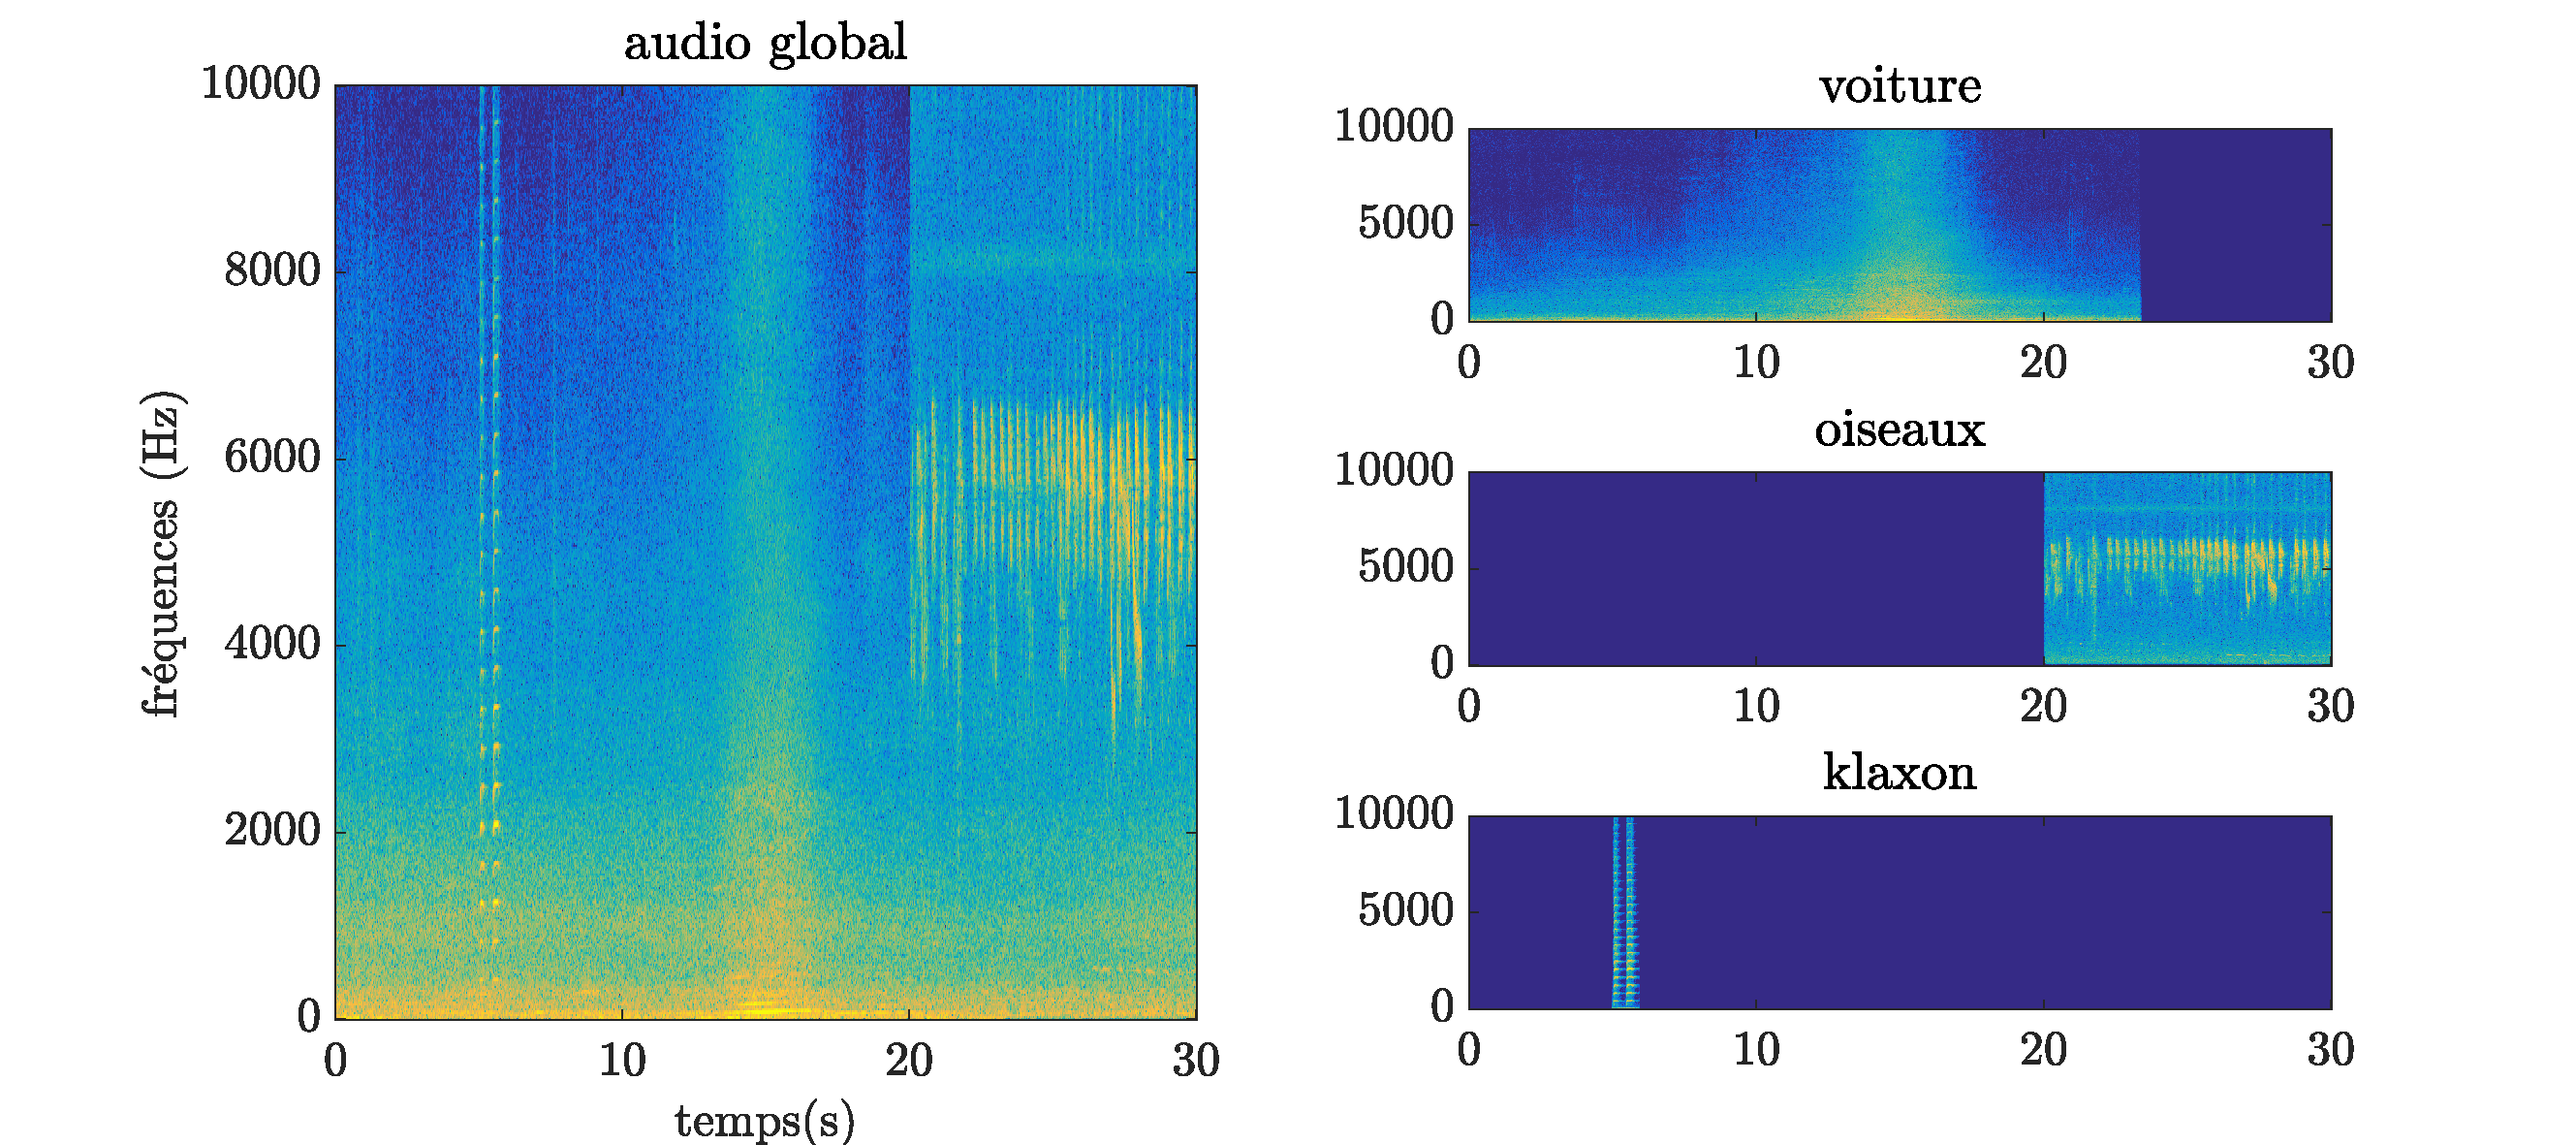
\includegraphics[width=.7\textwidth]{D:/gloaguen/Pictures/SimScene/exempleSimScene_spectrogramme_sourcesSonores.pdf}
\caption{Scène créée sous \textit{SimScene}. \`A gauche, le spectrogramme du signal global composé de trois sources (une voiture, un klaxon, un oiseau), à droite les spectrogrammes des trois sources audio utilisées}
\end{figure}


En parallèle, \textit{SimScene} génère 3 fichiers images (l'évolution temporelle du niveau sonore, le spectrogramme et un \textit{piano Roll} pour visualiser la répartition dans le fichier de chacune des classes, figure \ref{fig:somefiglabel}), un fichier texte résumant les temps de présence de l'ensemble des sons présents dans la scène et un fichier .\textit{mat} où se trouve la totalité des résultats et des paramètres de la scène.\\


\begin{figure}[ht]
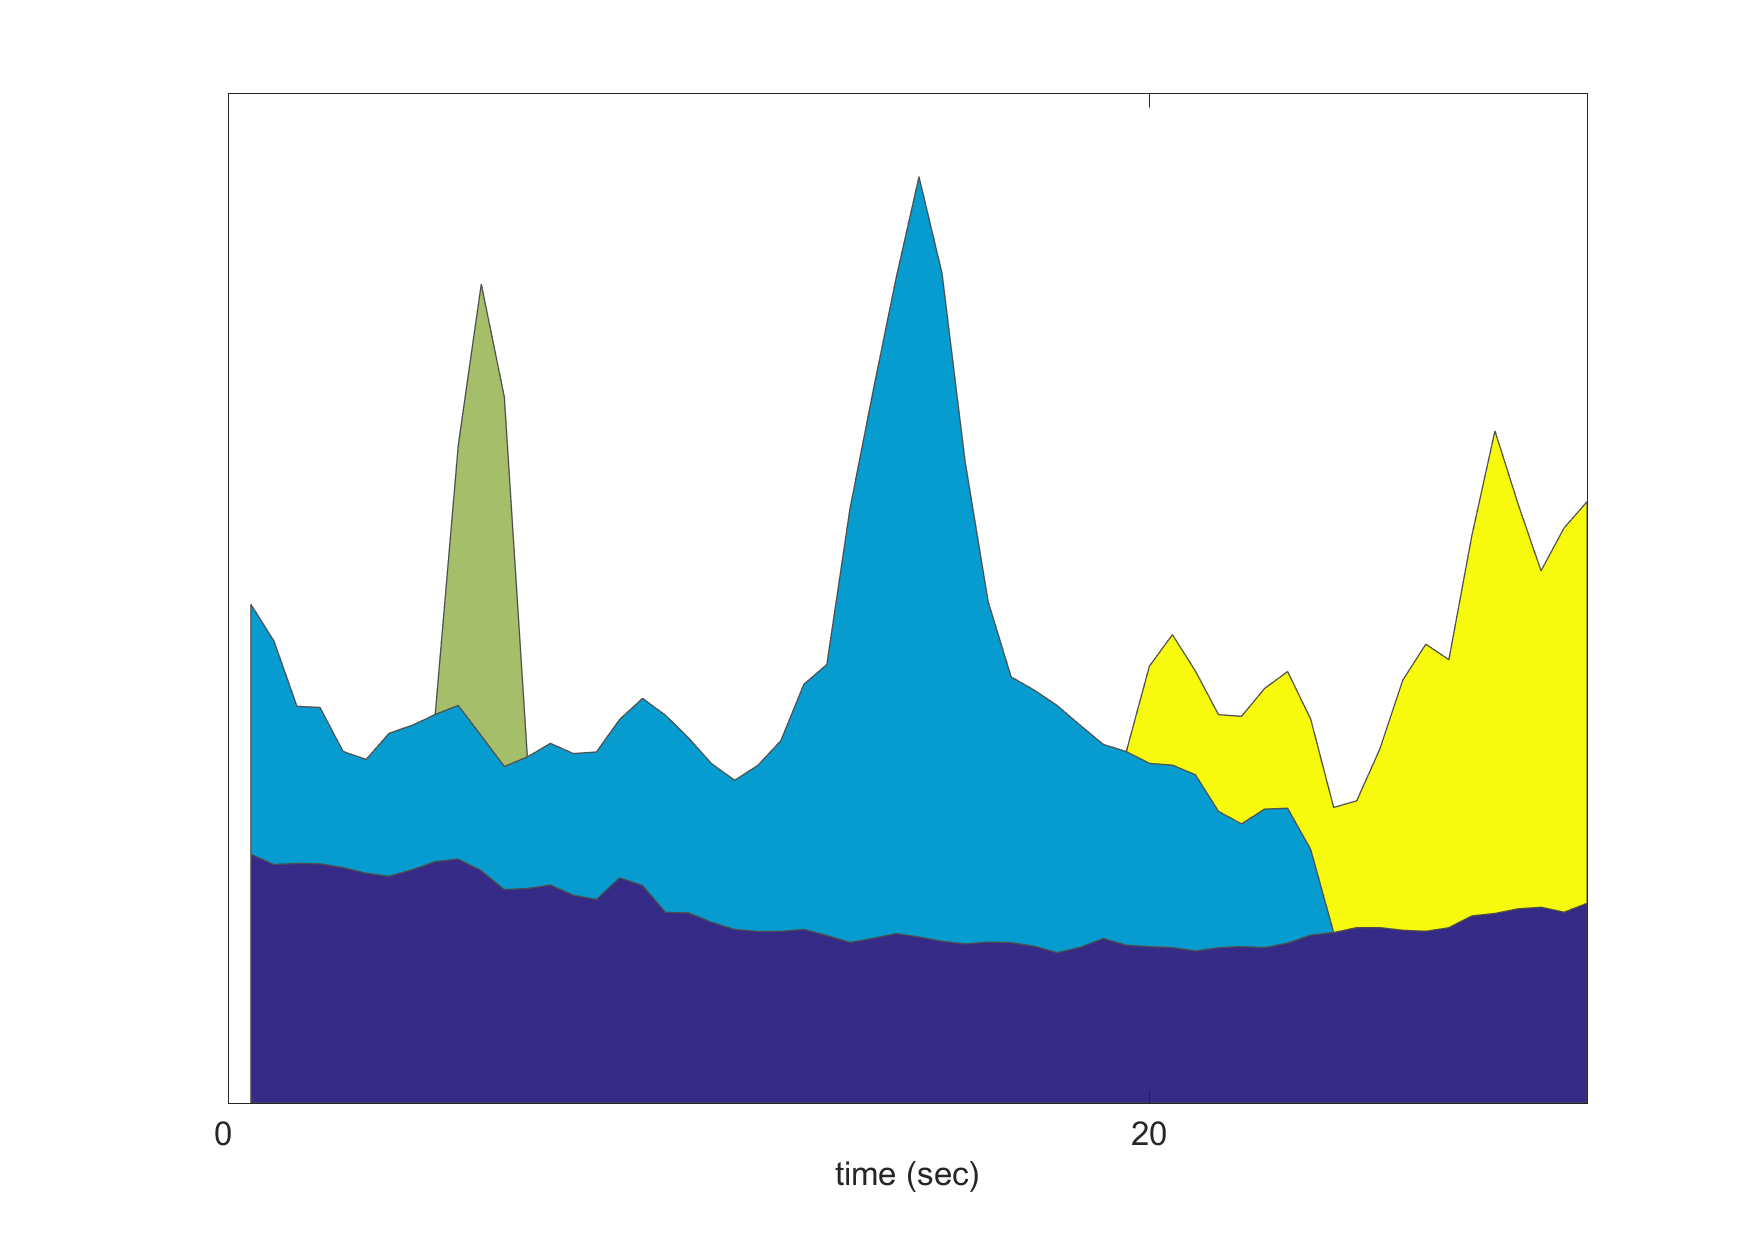
\includegraphics[width=5cm]{../../../Pictures/SimScene/exempleSimScene2-timeDomain.png}\hfill
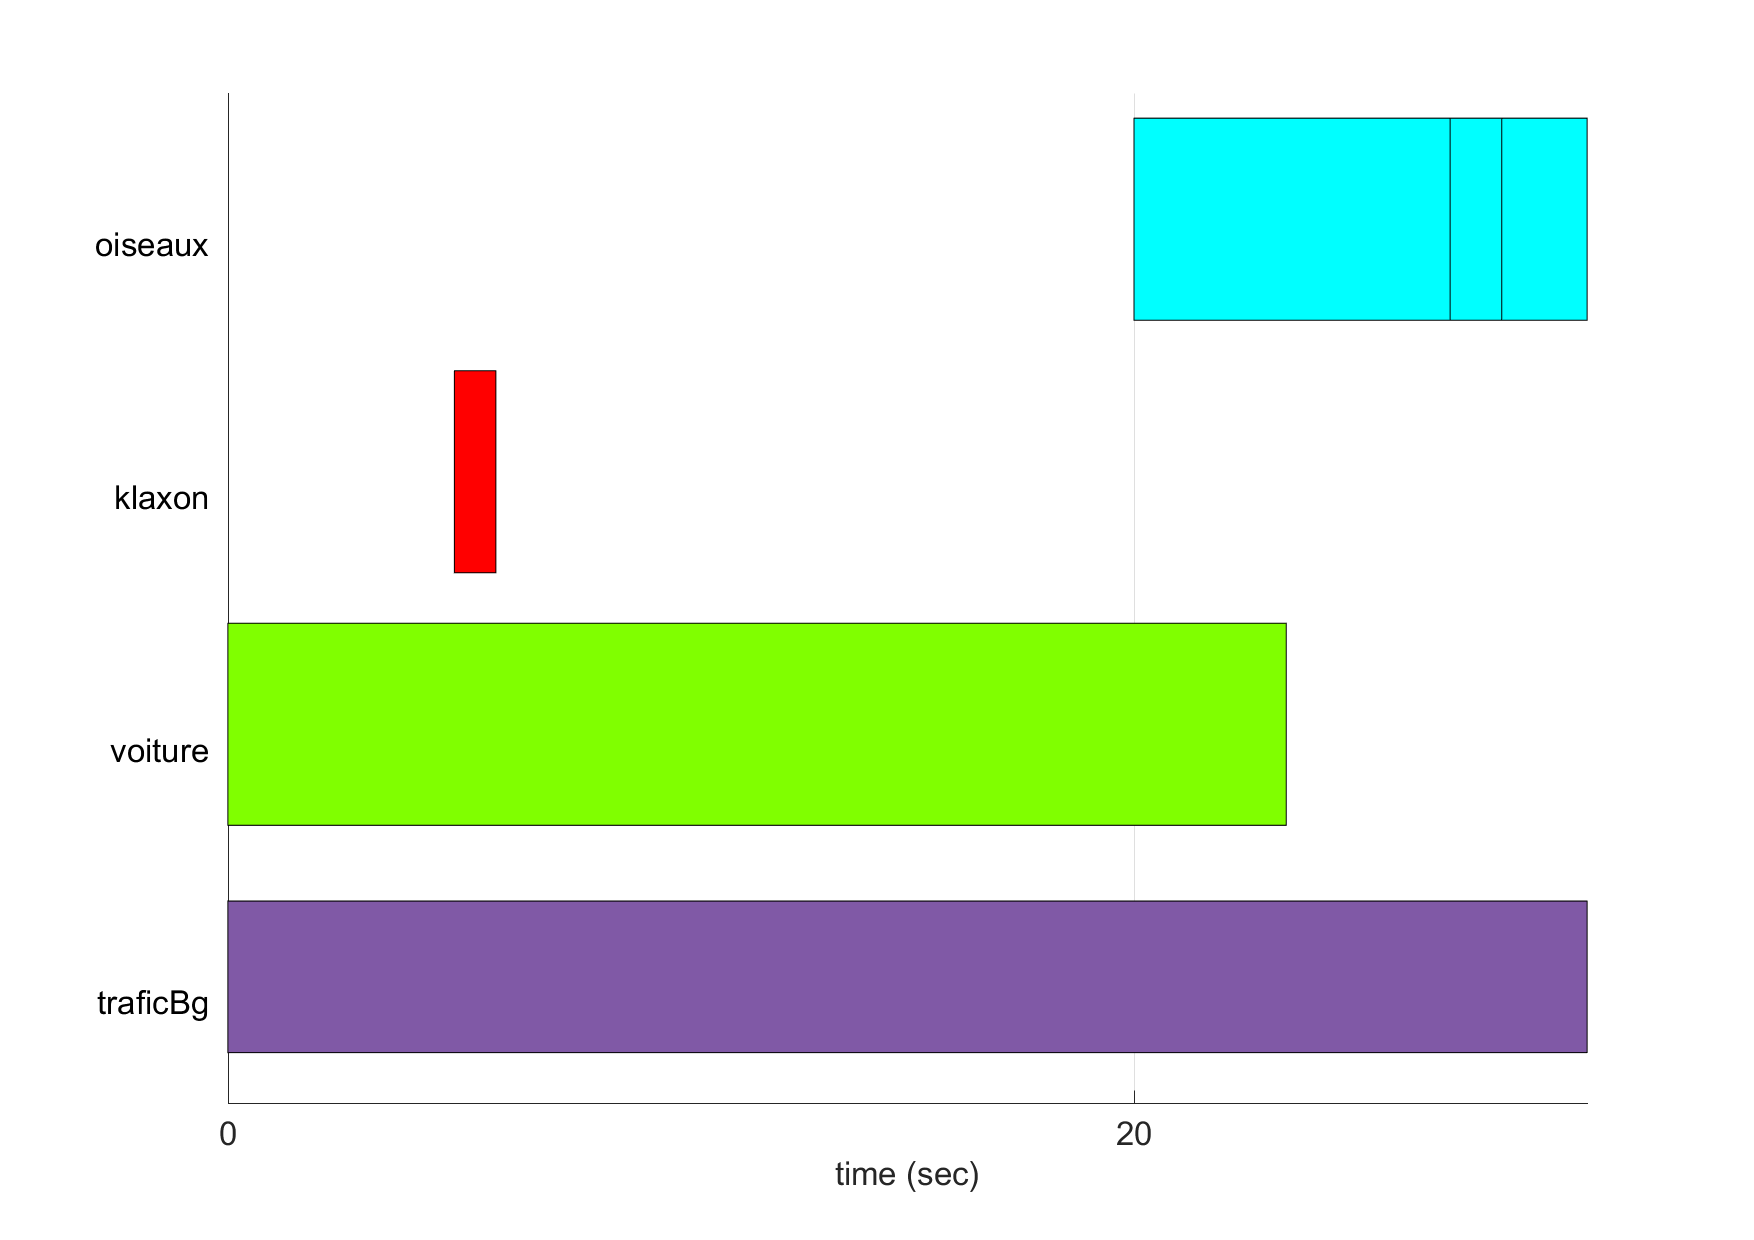
\includegraphics[width=5cm]{../../../Pictures/SimScene/exempleSimScene2-pianoRoll.png}\hfill
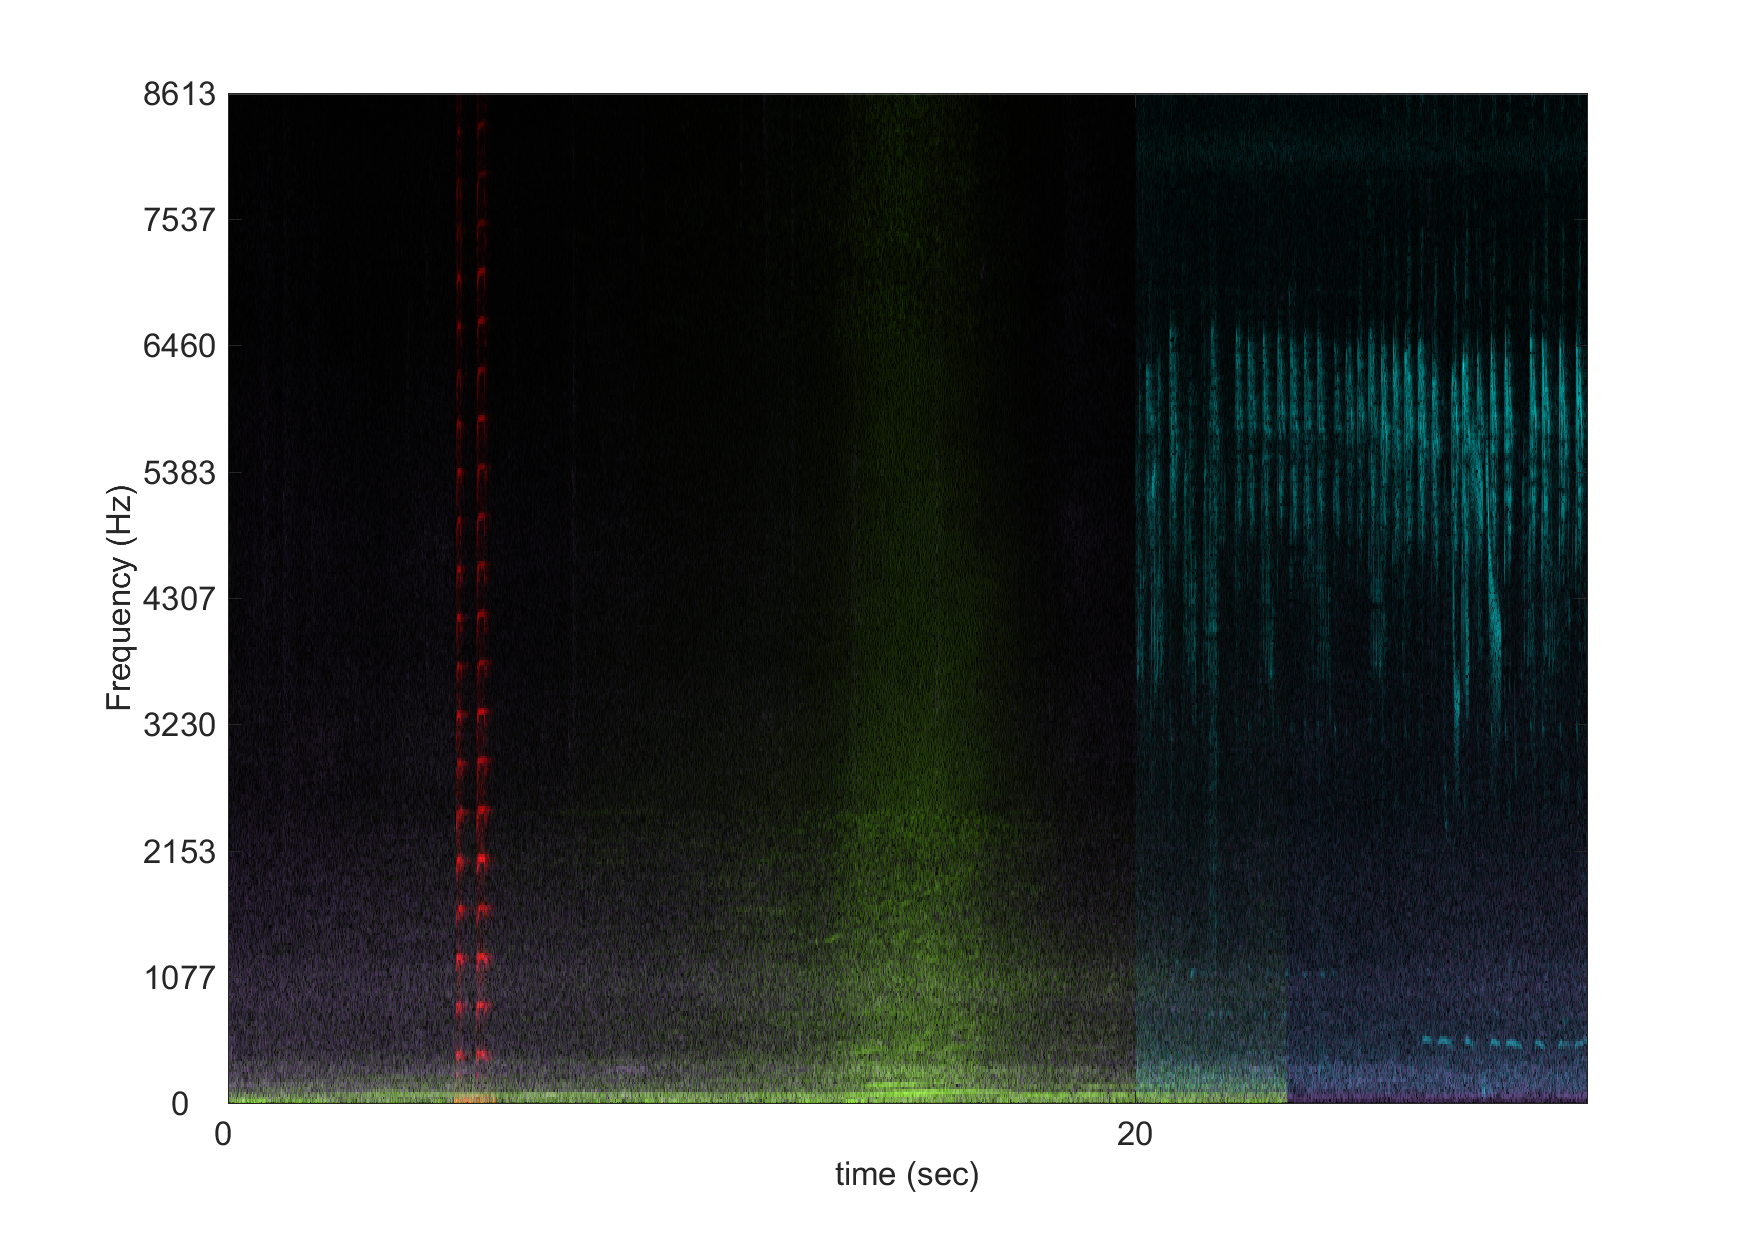
\includegraphics[width=5cm]{../../../Pictures/SimScene/exempleSimScene2-spectrum.png}
\caption{Représentation temporelle (à gauche), \textit{Piano Roll} (au centre) et spectrogramme (à droite) générés par \textit{SimScene}.}\label{fig:somefiglabel}
\end{figure}

La génération de scènes sous \textit{SimScene} peut se faire selon 2 modes. Dans le mode \textit{abstract}, l'utilisateur renseigne lui-même les échantillons sonores présents dans la scène et chaque paramètre permettant de créer des scènes complètement artificiels. \`A l'inverse, dans le mode \textit{replicate}, le schéma de la scène s'appuie sur un fichier texte où la position d'évènements sonore (début et fin) et leur classe de son correspondante sont détaillées. Ce mode permet de reproduire des scènes réelles annotées où la position de chaque évènement est connue.\\

Si \textit{SimScene} offre de nombreux paramètres pour créer de multiples scènes sonores variées, il nécessite d'avoir une base de données de sons isolés devant être suffisamment exhaustive. De plus, la qualité des audio doit être suffisante pour que la juxtaposition des sons ne viennent pas détériorer le rendu final (rapport Signal/Bruit élevé, échantillonnage à 44,1 kHz). Afin de réaliser au mieux des scènes sonores urbaines, des enregistrements sonores urbains sont étudiés. Ils permettent de connaitre les différentes ambiances sonores qui sont susceptibles d'exister en ville ainsi que les sources sonores qui les composent et enfin d'extraire les paramètres que \textit{SimScene} requiert (niveaux sonores, nombre d'occurrence d'une classe de son) pour réaliser des mixtures sonores en mode \textit{abstract} et les annotations nécessaire pour le mode \textit{replicate}. \\

\section{Études des scènes sonores urbaines}
\subsection{Présentation des scènes \textit{GRAFIC}}

Des enregistrements audio d'environnements sonores, réalisés dans le cadre du projet GRAFIC \cite{aumond_modelling_2017}, ont été récupérés. Ces audio ont été enregistrés à pied dans le 13\ieme~arrondissement de la ville de Paris sur un parcours comprenant 19 points d'arrêts (Figure \ref{fig:parcoursGRAFIC}). Le parcours définit présente l'avantage de couvrir plusieurs ambiances sonores représentatifs d'un environnement sonore urbain (Tableau \ref{tab:resume19pts}).\\
 
\begin{figure}[hbtp]
\centering
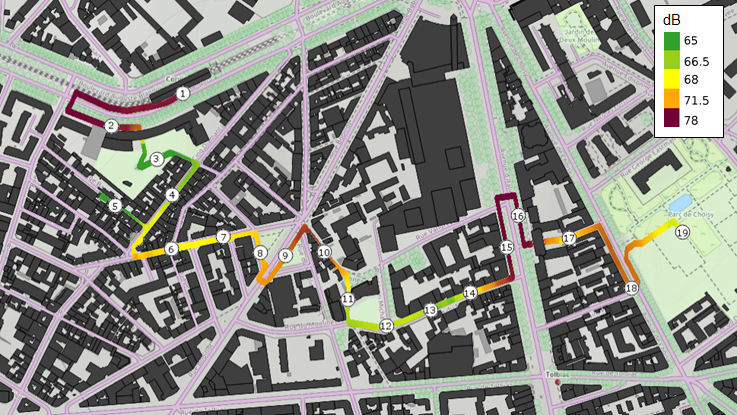
\includegraphics[width=.7\textwidth]{D:/gloaguen/Pictures/grafic/trajet_19pts.png}
\caption{Parcours réalisé par l'étude avec les 19 points de mesures avec le niveau sonore mesuré équivalent}
\label{fig:parcoursGRAFIC}
\end{figure}

Ce parcours a été réalisé sur deux jours (le 23/05/2015, jour 1, et le 30/05/2015, jour 2), deux fois par jour (le matin puis l'après-midi) dans un sens (d'est en ouest, EW) et dans l'autre (ouest en est, WE). L'enregistrement est réalisé par un système d'acquisition équipé d'un microphone ASASense omnidirectionnel situé sur un sac à dos porté par l'opérateur. En tout, 76 enregistrements audio de 1 à 4 minutes sont disponibles. \\

\begin{table}[h]
\centering

\begin{tabular}{|c|p{6cm}||c|p{6cm}|}
\hline
\textbf{Point} & \textbf{Description  }                 & \textbf{Point} & \textbf{Description                                      } \\ \hline
1     & Large rue à deux voies        & 10    & Rue sans trafic près d’une école                  \\ \hline
2     & Large rue à deux voies        & 11    & Rue silencieuse sans trafic                       \\ \hline
3     & Parc calme                    & 12    & Rue avec un faible débit de trafic                \\ \hline
4     & Rue animé avec restaurant/bar & 13    & Rue avec un faible débit de trafic                \\ \hline
5     & Rue très calme                & 14    & Rue avec un faible débit de trafic                \\ \hline
6     & Rue animé avec restaurant/bar & 15    & Rue avec un fort débit de trafic                  \\ \hline
7     & Rue animé avec restaurant/bar & 16    & Rue avec un fort débit de trafic                  \\ \hline
8     & Parc situé le long d’une rue  & 17    & Rue piétonne calme situé entre deux rues bruyante \\ \hline
9     & Rue avec un trafic modéré     & 18    & Grand carrefour avec un trafic constant           \\ \hline
      &                               & 19    & Grand parc                                        \\ \hline
\end{tabular}
\caption{résumé des 19 points de mesures avec l'ambiance générale}
\label{tab:resume19pts}
\end{table}


\subsection{Écoutes des scènes sonores}

La première étape établit un classement des enregistrements à partir des indications fournis dans \cite{aumond_modelling_2017} (résumé dans le Tableau \ref{tab:resume19pts}) et des écoutes faites selon quatre ambiances sonores (\textit{parc}, \textit{rue calme}, \textit{rue animée}, \textit{rue très animée}) comme défini par \cite{can_describing_2015} (Tableau \ref{tab:classificationScene}).\\

\begin{table}[t]
\caption{Classification des scènes par ambiances sonores.}
\centering
\begin{tabular}{|c|c|*{19}{l|}}
\hline
\multicolumn{1}{|l|}{\textbf{Jour}} & \textbf{trajet}   & 1                        & 2                        & 3                        & 4                        & 5                        & 6                        & 7                        & 8                        & 9                        & 10                       & 11                       & 12                       & 13                       & 14                       & 15                       & 16                       & 17                       & 18                       & 19                       \\ \hline
\textbf{1} & \textbf{EW} & \cellcolor[HTML]{F56B00} & \cellcolor[HTML]{F56B00} & \cellcolor[HTML]{5AB25A} & \cellcolor[HTML]{FFCB2F} & \cellcolor[HTML]{FFCB2F} & \cellcolor[HTML]{F56B00} & \cellcolor[HTML]{FFCB2F} & \cellcolor[HTML]{5AB25A} & \cellcolor[HTML]{F56B00} & \cellcolor[HTML]{5AB25A} & \cellcolor[HTML]{FFCB2F} & \cellcolor[HTML]{F56B00} & \cellcolor[HTML]{FFCB2F} & \cellcolor[HTML]{FFCB2F} & \cellcolor[HTML]{F56B00} & \cellcolor[HTML]{9A0000} & \cellcolor[HTML]{FFCB2F} & \cellcolor[HTML]{F56B00} & \cellcolor[HTML]{5AB25A} \\ \hline
\textbf{1}  & \textbf{WE} & \cellcolor[HTML]{F56B00} & \cellcolor[HTML]{F56B00} &                          & \cellcolor[HTML]{FFCB2F} & \cellcolor[HTML]{FFCB2F} & \cellcolor[HTML]{FFCB2F} & \cellcolor[HTML]{FFCB2F} & \cellcolor[HTML]{FFCB2F} & \cellcolor[HTML]{F56B00} & \cellcolor[HTML]{F56B00} & \cellcolor[HTML]{FFCB2F} & \cellcolor[HTML]{F56B00} & \cellcolor[HTML]{FFCB2F} & \cellcolor[HTML]{FFCB2F} & \cellcolor[HTML]{9A0000} & \cellcolor[HTML]{9A0000} & \cellcolor[HTML]{FFCB2F} & \cellcolor[HTML]{F56B00} &  \\ \hline
\textbf{2} & \textbf{EW} & \cellcolor[HTML]{F56B00} & \cellcolor[HTML]{F56B00} & \cellcolor[HTML]{5AB25A} & \cellcolor[HTML]{FFCB2F} & \cellcolor[HTML]{FFCB2F} & \cellcolor[HTML]{FFCB2F} & \cellcolor[HTML]{FFCB2F} & \cellcolor[HTML]{FFCB2F} & \cellcolor[HTML]{F56B00} & \cellcolor[HTML]{F56B00} & \cellcolor[HTML]{FFCB2F} & \cellcolor[HTML]{F56B00} & \cellcolor[HTML]{FFCB2F} & \cellcolor[HTML]{F56B00} & \cellcolor[HTML]{9A0000} & \cellcolor[HTML]{9A0000} & \cellcolor[HTML]{FFCB2F} & \cellcolor[HTML]{F56B00} & \cellcolor[HTML]{5AB25A} \\ \hline
\textbf{2} & \textbf{WE} & \cellcolor[HTML]{F56B00} & \cellcolor[HTML]{F56B00} & \cellcolor[HTML]{5AB25A} & \cellcolor[HTML]{FFCB2F} & \cellcolor[HTML]{FFCB2F} & \cellcolor[HTML]{FFCB2F} & \cellcolor[HTML]{FFCB2F} & \cellcolor[HTML]{FFCB2F} & \cellcolor[HTML]{F56B00} & \cellcolor[HTML]{FFCB2F} & \cellcolor[HTML]{FFCB2F} & \cellcolor[HTML]{FFCB2F} & \cellcolor[HTML]{FFCB2F} & \cellcolor[HTML]{FFCB2F} & \cellcolor[HTML]{9A0000} & \cellcolor[HTML]{9A0000} & \cellcolor[HTML]{FFCB2F} & \cellcolor[HTML]{9A0000} & \cellcolor[HTML]{5AB25A} \\ \hline
\end{tabular}

\vspace{0.5cm}


\begin{tabular}{|p{1.5cm}|l|p{0.001cm}|p{2cm}|l|p{0.001cm}|p{2cm}|l|p{0.001cm}|p{2.75cm}|l|p{0.001cm}|p{2.45cm}|l|}

\hhline{|-|-|~|-|-|~|-|-|~|-|-|~|-|-|}
Parc & {\cellcolor[HTML]{5AB25A}} & & Rue calme & {\cellcolor[HTML]{FFCB2F}} & & Rue animée & {\cellcolor[HTML]{F56B00}} & &  Rue très animée & {\cellcolor[HTML]{9A0000}} & & Non renseigné & \\
\hhline{|-|-|~|-|-|~|-|-|~|-|-|~|-|-|}

\end{tabular}
\label{tab:classificationScene}
\end{table}


Une majorité de scènes appartiennent à l'ambiance sonore \textit{rue calme} (36 scènes), 22 scènes appartiennent à l'ambiance \textit{rue animée} et 8 scènes à l'ambiance \textit{parc} et \textit{rue très animée}. Plus de la moitié des points de mesures possèdent la même ambiance sur les 4 trajets. A l'exception du point 10, les autres points de mesures possèdent deux ambiances sonores voisines. Ces variations peuvent provenir des variations d'activité dans la journée (matin ou l'après-midi). Enfin, les points 3 et 19 du parcours 1-WE ne sont pas exploitables : le point 3 est pollué par un camion balayeur et le point 19 n'a pas été correctement enregistré. Au final, c'est 74 fichiers audio qui sont disponibles. 

\subsection{Annotation}\label{part:scene_annotation}

L'annotation des enregistrements est ensuite réalisée. Il consiste à écouter chaque fichier audio et à estimer les sources sonores présentes ainsi que leur temps de présence (exemple en Tableau \ref{tab:exemple_annotation}). Pour chaque enregistrement, un fichier .txt résume ces informations.\\

\begin{table}[t]
\centering
\begin{tabular}{lll}
\textbf{évènements}    & $\mathbf{t_{init}}$ \textbf{(s)} & $\mathbf{t_{fin}}$ \textbf{(s)} \\ \hline
bruit rue     & 0,00            & 8,50           \\ \hline
voix          & 0,00            & 44,00          \\ \hline
camion        & 1,00            & 56,10          \\ \hline
voix          & 36,50           & 42,30          \\ \hline
voiture Ville & 52,00          & 63,00          \\ \hline
voix          & 59,00           & 66,50         
\end{tabular}
\caption{Exemple d'un fichier d'annotation pour la scène 1-EW-07}
\label{tab:exemple_annotation}
\end{table}


De ces annotations, il est alors possible d'estimer par ambiance sonore, un niveau sonore moyen, les classes de son qui caractérisent leur bruit de fond et également les classes de sons catégorisé en évènements sonores et leur densité (nombre d'évènement par minute). Ces informations sont alors suffisante pour pouvoir recréer ces scènes par le mode \textit{abstract} de \textit{SimScene} (Tableau \ref{tab:obsScene}). \\

\begin{table}
\centering
\begin{tabular}{L{2cm} | C{2cm} | C{2cm} | L{3cm} | C{2cm} | C{2cm}}
\toprule
\centering \small \textbf{Environnent sonore} & \small \textbf{Niveau sonore (dB)} & \small \textbf{Bruit de fond } & \small \centering \textbf{Évènement} & \small \textbf{Nombre évènement/min} & \small \textbf{Rapport Évènement-Bruit de fond (dB)} \\ \midrule

Parc              & 69,0        &
\begin{tabular}[c]{@{}l@{}}voix \\ sifflements \\ d'oiseaux \end{tabular} &
\begin{tabular}[c]{@{}l@{}}voiture ville \\ voix\\ sifflements\\ \hfill d'oiseaux \\ bruit de rue\\ bruit de pas\end{tabular}                                         &
\begin{tabular}[c]{@{}l@{}}1,6\\ 0,5 \\ 0,5 \\ \\ 0,5\\ 0,3\end{tabular}               &    \begin{tabular}[c]{@{}l@{}} 3,0 ($\pm$ 6,0) \\ 6,5 ($\pm$ 5,0) \\ 0,0 ($\pm$ 9,5) \\	\\ 6,7 ($\pm$ 4,5) \\ 4,0 ($\pm$ 7,0)\end{tabular}     \\\hline

Rue calme      & 70,2        &
\begin{tabular}[c]{@{}l@{}}trafic routier\\ \begin{tabular}[c]{@{}l@{}}sifflements \\ \hfill d'oiseaux \end{tabular}\end{tabular}       &
\begin{tabular}[c]{@{}l@{}}voiture ville \\ voix\\ bruit de rue\\ bruit de pas\\ sifflements \\ \hfill d'oiseaux \\  porte de maison\\ porte de voiture \\chantier \end{tabular} &
\begin{tabular}[c]{@{}l@{}}1,7\\ 0,7\\ 0,7\\ 0,5\\ 0,2\\  \\  0,2\\ 0,2 \\  0,1\end{tabular} & \begin{tabular}[c]{@{}l@{}} 7,6 ($\pm$ 4,6) \\ 8,2 ($\pm$ 4,0) \\ 7,6 ($\pm$ 4,2) \\ 8,0 ($\pm$ 5,0) \\ 3,0 ($\pm$ 5,8) \\ \\ 9,0 ($\pm$ 3,3) \\ 7,7 ($\pm$ 4,2) \\ 3,7 ($\pm$ 5,1) \end{tabular}
\\ \hline

Rue animée      & 73,5        & trafic routier                                                      & \begin{tabular}[c]{@{}l@{}}voiture ville \\ voix\\ bruit de pas\\ bruit de rue \\ klaxon\\ sifflements \\ \hfill d'oiseaux \\ porte de voiture\\ sirène \\ sonnette\end{tabular}                   & \begin{tabular}[c]{@{}l@{}}9,4 \\ 0,6 \\ 0,5\\ 0,4 \\ 0,3\\ 0,2\\ \\ 0,2\\ 0,1 \\ 0,1\end{tabular}  & \begin{tabular}[c]{@{}l@{}} 3,3 ($\pm$ 2,5) \\ 1,3 ($\pm$ 2,6) \\ -3,6 ($\pm$ 6,4) \\ 5,2 ($\pm$ 4,6) \\ 3,5 ($\pm$ 3,9)\\ 1,6 ($\pm$ 5,0)  \\ \\ 4,4 ($\pm$ 5,4) \\ 2,0 ($\pm$ 6,2) \\ 1,7 ($\pm$ 3,5) \end{tabular}\\ \hline

Rue très animée & 76,0 & trafic routier                                                      &
\begin{tabular}[c]{@{}l@{}}voiture ville\\ voix \\ klaxon \\ porte de voiture\\ sirène\\ bruit de pas\\ bruit de rue\end{tabular}                          
& 
\begin{tabular}[c]{@{}l@{}}40,9\\ 0,3\\ 0,3\\ 0,3\\ 0,2\\ 0,2\\ 0,2\end{tabular}  & \begin{tabular}[c]{@{}l@{}}2,3 ($\pm$ 1,3) \\ 1,3 ($\pm$ 1,1) \\ 2,7 ($\pm$ 4,1) \\ 3,6 ($\pm$5,4) \\ -3,0 ($\pm$ 4,2) \\ -3,6 ($\pm$ 5,8) \\ 5,1 ($\pm$ 4,7) \end{tabular}\\ \bottomrule
\end{tabular}
\caption{Niveau sonore et description des classes de sons les plus récurrentes dans l'environnement urbain (nombre d'évènements sonore par minute > 0.1/min).}
\label{tab:obsScene}
\end{table}



Sur l'ensemble des scènes sonores, XX classes de sons sont identifiés : . La classe de son \textit{bruit rue} résume les nombreux bruits, le plus souvent très bref, dont la source sonore n'a pas pu être déterminée. De la même façon, les sons relatifs à un chantier en construction (marteau-piqueur, marteau, perceuse) sont regroupés en une seule classe par soucis de simplification. Les sources sonores les plus communes sont \textit{voiture}, \textit{voix} et \textit{bruit rue}. En outre, en plus des classes de sons résumées dans le Tableau \ref{tab:obsScene}, de nombreuses autres classes de sons (\textit{aboiement de chien},\textit{bruit de balais}, \textit{toussotement}, \textit{passage d'avion}, \textit{roulement de valise}) entendus interviennent plus sporadiquement (nombre d'évènement/min < 0,1) et sont susceptibles d'intervenir dans les quatre ambiances sonores.

On observe une évolution générale des classes de son avec l'augmentation du niveau sonores des ambiances : plus la rue est bruyante plus la part de la classe \textit{trafic} et celles de l'activité humaine (\textit{voix, bruit de pas}) sont prédominantes. À l'inverse, les classes de sons \og naturel \fg{} (\textit{oiseaux)} disparaissent progressivement.

Notons que dans \textit{rue calme}, \textit{bruyante} et dans \textit{parc}, le décompte des voitures est assez aisé, il l'est moins dans \textit{rue très bruyante} où c'est plus un flot, parfois continu, de véhicules qui est présent, le comptage y est alors très délicat car les véhicules peuvent être considérés à la foi comme bruit de fond et évènements sonore. Ainsi, lorsque le flux de véhicule est trop important, on considère en moyenne 1 véhicule par seconde. Ce nombre est donc soumis à une forte incertitude mais reste cependant cohérent avec les indications du débit moyen fournis dans \cite{aumond_modelling_2017}.\\

Ces observations (ambiances sonores, classes de sons présents par ambiance, débit de voiture) et ces annotations permettent ensuite de réaliser des mixtures sonores urbaines respectivement avec le mode \textit{abstract} ou avec le mode \textit{replicate}. Le relevé des différentes classes de sons sert ensuite à générer une base de données de sons afin réaliser des scènes.

\section{Création d'une base de données}

\subsection{Constitution des évènements et des bruits de fond sonores}

La base de données de sons pour \textit{SimScene} comprend un ensemble de classes de sons isolés (oiseaux, voiture, klaxon  \dots) qui contiennent chacune plusieurs échantillons (\textit{oiseaux01.wav}, \textit{oiseaux02.wav} \dots) pour permettre une grande variabilité dans les mixtures sonores créées. La plupart des échantillons sont trouvés sur des sites en ligne de sons \footnote{\url{www.freesound.org}} \footnote{\url{www.universalsoundbank.com}} et à l'aide de la base de données constituée par J. Salamon et al. \cite{salamon_dataset_nodate}. Leur base de données comprend en tout plus de 8000 fichiers audio, collectés également sur le site \textit{freesound.org}, d'une durée inférieure à 4 secondes répartit en 10 classes de sons : ventilation, klaxon de voiture, enfants qui joue, chien qui aboie, sonnerie, moteur en fonctionnement, coup de feu, marteau-piqueur, sirène et musique dans la rue. L'ensemble des échantillons a été trié afin de ne conserver que les audio ayant un rapport signal à bruit grand et un échantillonnage de 44,1 kHz minimum.\`A partir de la liste des noms des fichiers originaux fournis avec cette base de données, les fichiers audio sont récupérés dans leur intégralité sur le site internet et intégrés dans la base de données.\\
Afin d'obtenir un rapport signal à bruit acceptable, certains audio ont été filtrés à l'aide du logiciel d'Audacity par un filtre de Wiener. D'autres signaux ont, quant à eux, été tronqués ou bien divisés en plusieurs fichiers afin d'obtenir des durées convenables. 
 
\subsection{Enregistrements de passages de véhicules}
S'il est possible de trouver l'ensemble des classes de son dans une qualité suffisante en ligne, dans le cas de la classe \textit{voiture}, il nous a semblé utile de réaliser des enregistrements de passages de véhicules sur une piste d'essai afin de posséder un ensemble varié et maitrisé de vitesses et de modèles de véhicules. Pour cela, 4 voitures ont été testé (Renault Mégane, Renault Clio, Renault Sénic et Dacia Sandero) en suivant un plan de mesure comprenant plusieurs vitesses stabilisées pour différents rapports de vitesses et en phase d'accélération et de freinage.
Photo et moteur ??

\begin{table}[!htb]
    \begin{minipage}{.5\linewidth}
      \centering
        \begin{tabular}{|c|c|lllll}
\cline{2-7}
\multicolumn{1}{l|}{} & \multicolumn{1}{l|}{\textbf{Rapport}} & \multicolumn{1}{l|}{\textbf{1}} & \multicolumn{1}{l|}{\textbf{2}} & \multicolumn{1}{l|}{\textbf{3}} & \multicolumn{1}{l|}{\textbf{4}} & \multicolumn{1}{l|}{\textbf{5}} \\ \hline
\multicolumn{1}{|c|}{\multirow{8}{*}{\begin{tabular}[c]{@{}c@{}}\textbf{Vitesse}\\   \textbf{stabilisée}\\   \textbf{(km/h)}\end{tabular}}} & \textbf{20} & \multicolumn{1}{l|}{$\times$} & \multicolumn{1}{l|}{} & \multicolumn{1}{l|}{} & \multicolumn{1}{l|}{} & \multicolumn{1}{l|}{} \\ \cline{2-7} 
\multicolumn{1}{|c|}{} & \textbf{30} & \multicolumn{1}{l|}{} & \multicolumn{1}{l|}{$\times$} & \multicolumn{1}{l|}{$\times$} & \multicolumn{1}{l|}{} & \multicolumn{1}{l|}{} \\ \cline{2-7} 
\multicolumn{1}{|c|}{} & \textbf{40} & \multicolumn{1}{l|}{} & \multicolumn{1}{l|}{$\times$} & \multicolumn{1}{l|}{$\times$} & \multicolumn{1}{l|}{$\times$} & \multicolumn{1}{l|}{} \\ \cline{2-7} 
\multicolumn{1}{|c|}{} & \textbf{50} & \multicolumn{1}{l|}{} & \multicolumn{1}{l|}{} & \multicolumn{1}{l|}{$\times$} & \multicolumn{1}{l|}{$\times$} & \multicolumn{1}{l|}{} \\ \cline{2-7} 
\multicolumn{1}{|c|}{} & \textbf{60} & \multicolumn{1}{l|}{} & \multicolumn{1}{l|}{} & \multicolumn{1}{l|}{} & \multicolumn{1}{l|}{$\times$} & \multicolumn{1}{l|}{$\times$} \\ \cline{2-7} 
\multicolumn{1}{|c|}{} & \textbf{70} & \multicolumn{1}{l|}{} & \multicolumn{1}{l|}{} & \multicolumn{1}{l|}{} & \multicolumn{1}{l|}{$\times$} & \multicolumn{1}{l|}{$\times$} \\ \cline{2-7} 
\multicolumn{1}{|c|}{} & \textbf{80} & \multicolumn{1}{l|}{} & \multicolumn{1}{l|}{} & \multicolumn{1}{l|}{} & \multicolumn{1}{l|}{} & \multicolumn{1}{l|}{$\times$} \\ \cline{2-7} 
\multicolumn{1}{|c|}{} & \textbf{90} & \multicolumn{1}{l|}{} & \multicolumn{1}{l|}{} & \multicolumn{1}{l|}{} & \multicolumn{1}{l|}{} & \multicolumn{1}{l|}{$\times$} \\ \hline
\textbf{Total} & 14 &  &  &  &  &  \\ \cline{1-2}
\end{tabular}
    \end{minipage}
    \begin{minipage}{.5\linewidth}
      \centering
\begin{tabular}{|c|c||c|c|}
\hline
\multicolumn{2}{|c||}{\textbf{Freinage}} & \multicolumn{2}{c|}{\textbf{Accélération}} \\ \hline
\multicolumn{1}{|c|}{\begin{tabular}[c]{@{}c@{}}\textbf{Vitesse}\\  \textbf{(km/h)}\end{tabular}} & \multicolumn{1}{c||}{\textbf{Rapport}} & \multicolumn{1}{c|}{\begin{tabular}[c]{@{}c@{}}\textbf{Vitesse}\\  \textbf{(km/h)}\end{tabular}} & \multicolumn{1}{c|}{\textbf{Rapport}} \\ \hline
50 → 0 & 3 → 2 & 0 → 30 & 1 → 2 \\ \hline
40 → 0 & 2 → 2 & 0 → 40 & 1 → 2 \\ \hline
50 → 30 & 3 → 2 & 20 → 40 & 1 → 3 \\ \hline
60 → 40 & 4 → 3 & 30 → 50 & 2 → 3 \\ \hline
70 → 50 & 4 → 3 & 40 → 60 & 3 → 4 \\ \hline
80 → 50 & \begin{tabular}[c]{@{}l@{}}4 ou 5\\ → 3\end{tabular} & 50 → 70 & \begin{tabular}[c]{@{}l@{}}3 → \\ 4 ou 5\end{tabular} \\ \hline
\end{tabular}
    \end{minipage}%
    \caption{Ensemble de mesures réalisées sur pistes avec des passages de véhicules à vitesses stabilisée (à gauche) et en accélération et freinage (à droite)} 
\end{table}

Les enregistrement ont été réalisé sur la piste d'essais de l'Ifsttar de Nantes le 7 et 8 juillet 2016 à l'aide du système d'acquisition A COMPLETER, la position du microphone a respecté la norme A COPLETER et fut donc situé à 7m de la piste à une hauteur de 1m50. Enfin, les conditions météorologiques étaient satisfaisantes (temps clar et dégagée, température à l'ombre de 25$/°$ C , vitesse moyenne du vent inférieure à 2 m/s). Les enregistrements sont ensuite extraits en fichiers audio en format .wav échantillonnés à 44,1 kHz.
 
En raison de la présence d'arbres situés proche de la piste, de nombreux oiseaux ont été enregistrés détériorant la qualité des fichiers audio. Afin d'atténuer leur présence, un filtre médian a été appliqué sur leur spectrogramme \cite{fitzgerald_drum_2010} dans la bande de fréquence $\left[2500 - 6500\right]$ Hz, correspondante aux fréquences d'émission des oiseaux. Ce filtre consiste a définir une fenêtre et à attribuer la valeur médiane de cette fenêtre à l'élément central. Puisque les aspects à la fois temporel et fréquentiel sont à prendre en compte, le fenêtre du filtre est de forme rectangulaire de taille $5 \times 9$ (96 Hz $\times$ 230 ms).\\

\begin{figure}[hbtp]
\centering
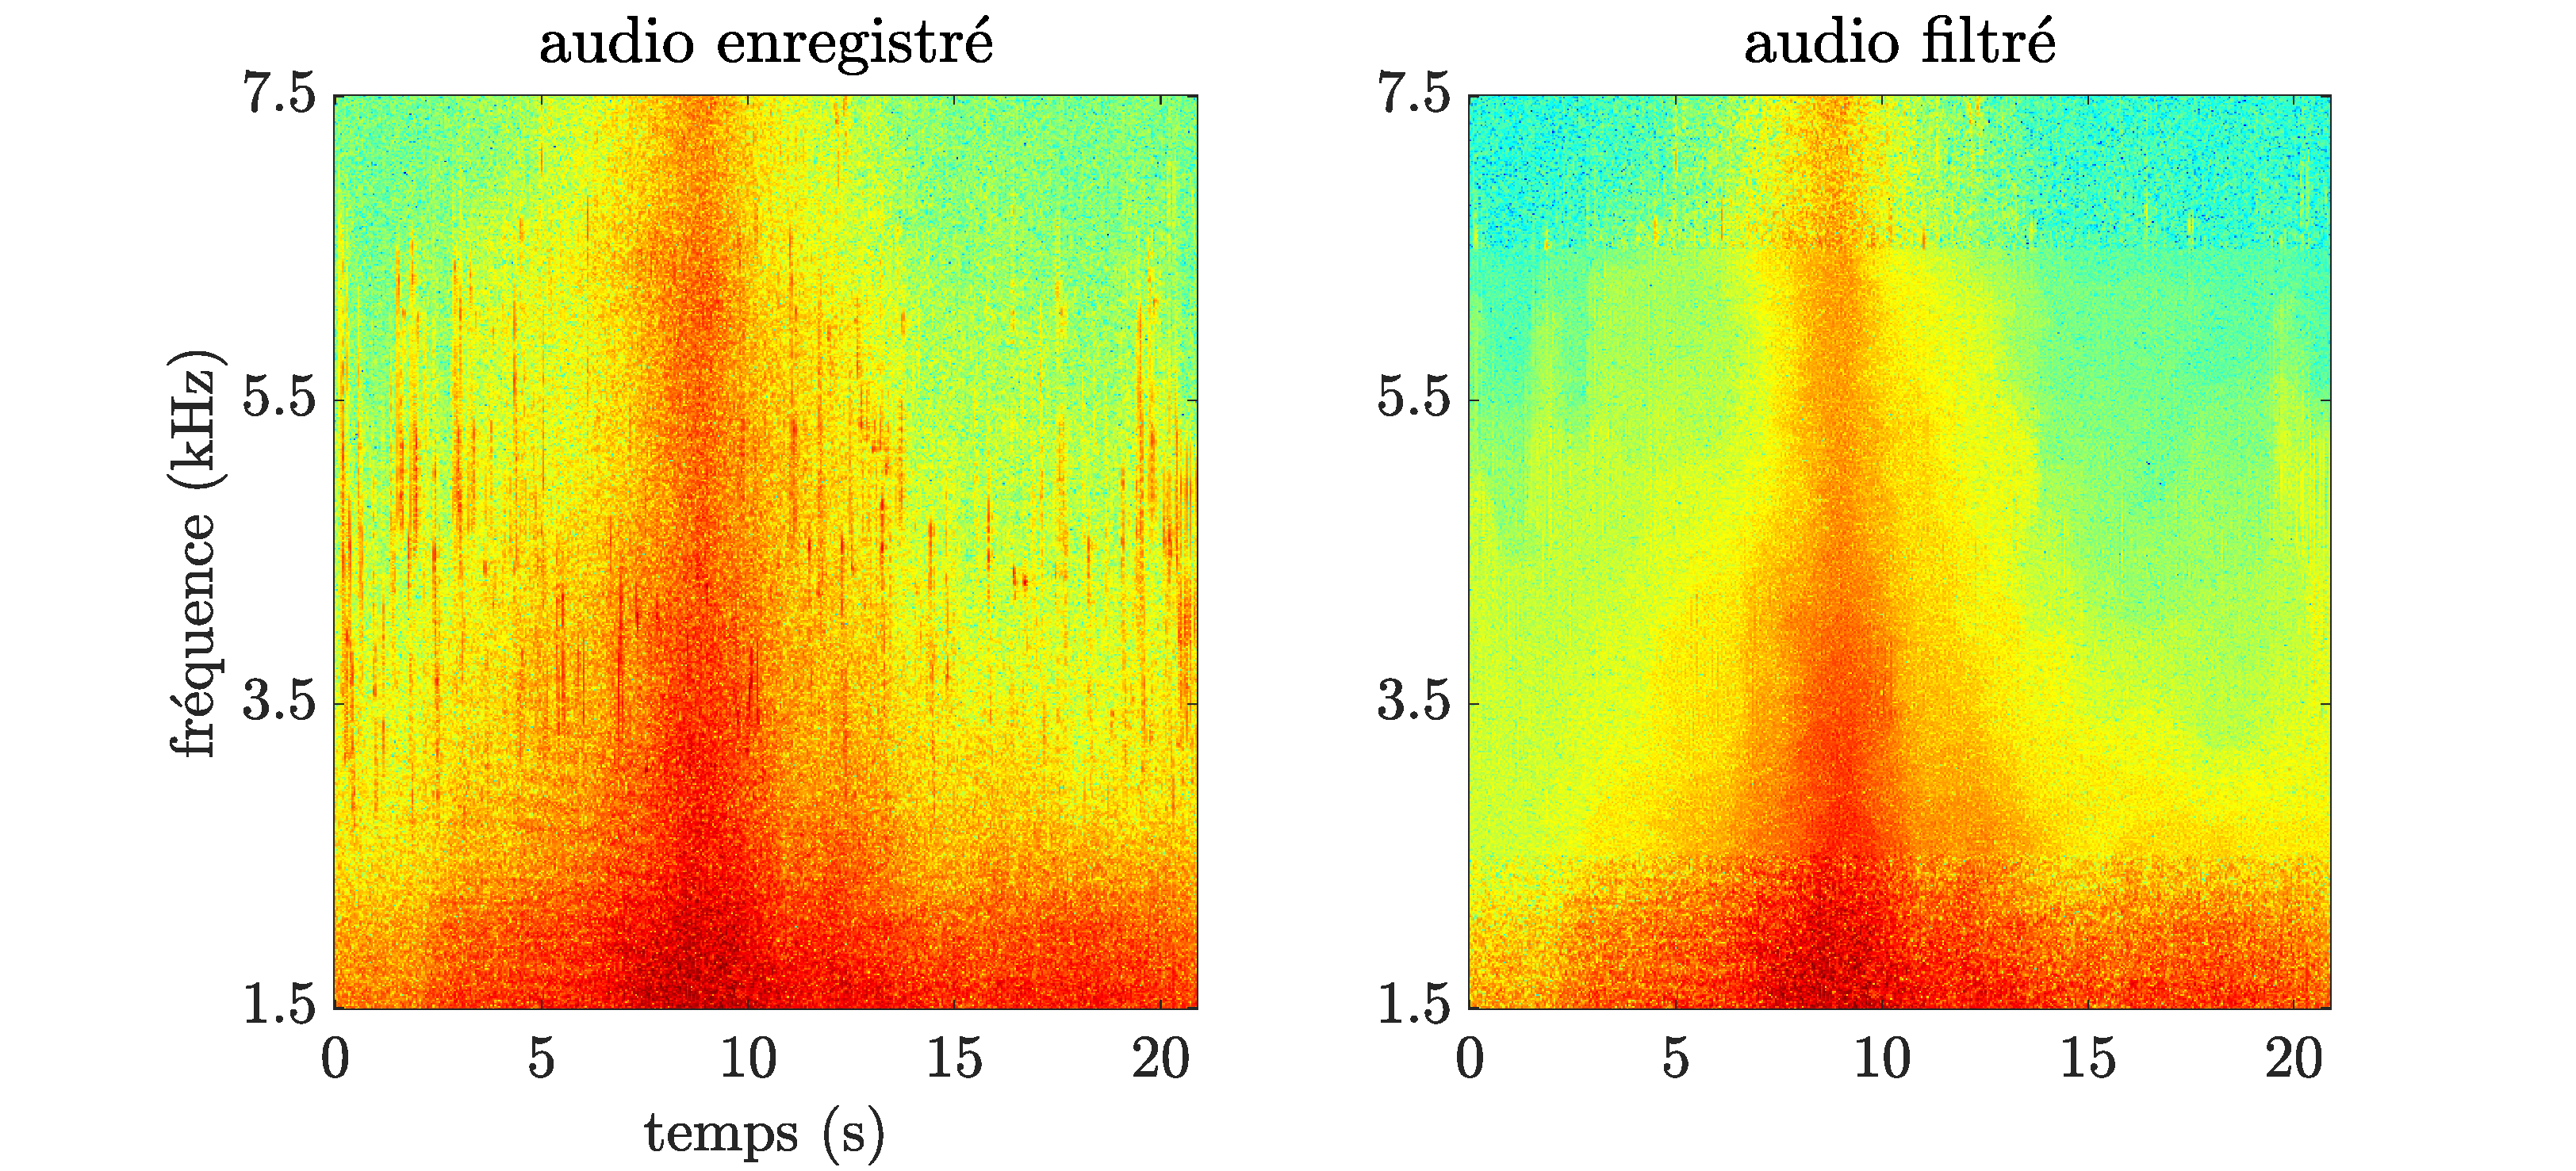
\includegraphics[width=.9\textwidth]{../../../Pictures/autres/filtrageMedian_VL1_R3_40_FR.pdf}
\caption{Zoom du spectrogramme (fenêtre $W = 2^{12}$, $nfft = 2^{12}$, overlapping = 50 $\%$) dans la bande de fréquence $\left[1500-7500 \right]$ Hz d'un enregistrement de passage de véhicule (véhicule Renault, rapport 3, 40 km/h). \`A gauche, l'enregistrement original, à droite l'enregistrement filtré par le filtre médian.}
\end{figure}


La présence des oiseaux est alors fortement atténué (même si elle reste, sur certains enregistrements, persistante) sans toutefois dégrader le passage du véhicule. Leur utilisation est donc possible sans diminuer la qualité des scènes simulées.\\

\subsection{Base de données complète}
La base de données comprend alors des évènements sonores court allant de 1 secondes (klaxon, aboiement de chien) à plusieurs dizaines de secondes (passages de voiture, sirènes d'ambulances). Ces éléments permettent de créer du dynamisme sonore dans la scène et sont les évènements sonores qu'on peut annoter dans une scène. Elle comprend également des sons de durées plus longues (1 min à 2 min) qui vont permettre de générer une bruit de fond sonore utile à la création de l'ambiance sonore générale de la scène (oiseaux, voix d'enfant dans une cours de récréation, trafic routier continu...). Les enregistrements des passages de voitures sont séparés en deux catégories : \textit{ville} et \textit{route}. Dans la première catégorie, se trouve toutes les voitures ayant une vitesse stabilisée ou finale inférieure à 50 km/h et dans la seconde, une vitesse stabilisée ou finale supérieure ou égale à 50 km/h. L'ensemble des fichiers audio est en format .wav échantillonnés à 44,1 kHz. La base de données finales est résumée dans le tableau \ref{tab:dataBaseEv} pour les évènements sonores et dans le tableau \ref{tab:dataBaseBcg} pour les bruits de fond sonores. 

\begin{table}[h]
\centering
\begin{tabular}{m{5cm} c |m{5cm} c}
\hline
\toprule
\textbf{Classe de son} & \textbf{Nombre} & \textbf{Classe de son} & \textbf{Nombre} \\
\midrule
Aboiement de chien & 34 & Porte de voiture & 5\\ 
\rowcolor[HTML]{C0C0C0}
Balais & 6 & Roulement de valise & 5 \\ 
Bruit de chantier (marteau, perceuse \dots) & 12 & Sirène & 9 \\ 
\rowcolor[HTML]{C0C0C0}
Bruit de rue & 24 & Sonnette & 5 \\ 
Camion & 4 & Toussotement & 7\\ 
\rowcolor[HTML]{C0C0C0}
Cloches d'églises & 8 & Train & 7 \\ 
Klaxon & 24 & Tram & 7 \\
\rowcolor[HTML]{C0C0C0}
Oiseaux & 30 & Voiture à l'arrêt & 7 \\ 
Orage & 3 & Voiture ville & 28 \\ 
\rowcolor[HTML]{C0C0C0}
Pas dans la ville & 11 & Voiture route & 16 \\ 
Pas dans un parc & 16 & Voix (rire, 1 ou 2 mots) & 24 \\
\rowcolor[HTML]{C0C0C0}
Porte de maison & 5 &  \textbf{Total} & \textbf{321}\\ 
\bottomrule
\end{tabular}
\caption{Composition de la base de données pour les évènements sonores}
\label{tab:dataBaseEv}
\end{table}

\begin{table}[h]
\centering
\begin{tabular}{m{5cm} c |m{5cm} c}
\toprule
\textbf{Classe de son} & \textbf{Nombre} & \textbf{Classe de son} & \textbf{Nombre} \\ \midrule
Brouhaha de foule & 15 & Pluie & 14 \\ 
\rowcolor[HTML]{C0C0C0}
Brouhaha parc & 25 & Trafic routier & 9 \\
Chantier & 28 & Vent dans les arbres & 15 \\ 
\rowcolor[HTML]{C0C0C0}
Cours de récréation & 12 & Ventilation & 10 \\ 
Oiseaux & 25 & \textbf{Total} & \textbf{153} \\ 
\bottomrule
\end{tabular}
\caption{Composition de la base de données pour les bruits de fond}
\label{tab:dataBaseBcg}
\end{table}


L'annotation des scènes GRAFIC et la base de données permettent maintenant de reconstituer ces scènes.

\section{Reproduction des scènes réelles}

Afin d'obtenir des scènes les plus réalistes possibles, le choix a été fait de reproduire les 74 enregistrements à l'aide de leur annotation et du mode \textit{replicate} de \textit{SimScene}. Ce choix permet ainsi de s'assurer que la disposition des évènements sonores dans les mixtures sonore s'est déjà produite. La difficulté réside surtout dans l'estimation du \textit{SNR} pour les évènements sonores qui doit être cohérent par rapport à l'ambiance souhaitée. Son estimation et sa variance s'est donc faite empiriquement et a été ajusté progressivement en fonction du rendu obtenu. Le niveau sonore global de la scène simulée est enfin modifié pour être similaire à celui de la scène réelle.\\

Dans la suite du document, les scènes issues du mode \textit{replicate} de \textit{SimScene} seront appelées \og scènes répliquées \fg{} en raison du processus de duplication. Les scènes originelles sont quant à elle nommées \og scènes enregistrées \fg{}.


\section{Tests perceptifs}\label{sec:test}

Afin de vérifier que le rendu global des scènes répliquées est suffisamment réaliste pour être similaire à des enregistrements faits en ville, celle-ci sont soumises à un test perceptif. Ce test consiste à faire écouter, à un panel d'auditeurs, un ensemble de scènes sonores comprenant autant d'enregistrements sonores que de scènes reconstitués. À chaque scène, l'auditeur doit alors évaluer, sur une échelle de Likert à 7 points allant de \og très peu réaliste \fg{} à \og extrêmement réaliste \fg{}, le réalisme de la scène qu'il vient d'entendre. L'objectif est que l'ensemble des scènes répliquées soient perçues de façon similaire aux scènes réalistes.\\

\subsection{Mise en place du test}
\label{sec:test_BEI}

Sur l'ensemble des 148 scènes (74 réelles, 74 répliquées),  un ensemble de 40 scènes d'une durée de 30 secondes sont testés. Cet ensemble est composé pour moitié de scènes réelles et des même scènes répliquées. L'hypothèse faite est que si les 20 scènes répliquées sont perçues de la même manière que les 20 scènes enregistrées, le réalisme peut être étendu aux 54 autres scènes répliquées. 

Dans un premier temps, 20 scènes enregistrées ont été choisis aléatoirement parmis les 74 enregistrements tout en prenant soin d'avoir une répartition équitable entre les ambiance sonores afin d'avoir suffisamment de diversité sonore. On extrait alors 5 scènes issus d'une ambiance \textit{Parc}, 6 issus de \textit{Rue calme}, 4 de \textit{Rue animée} et 5 de \textit{Rue très animée}  dans les échantillons. Pour chaque audio, 30 secondes sont ensuite sélectionnés aléatoirement. Puis, dans un second temps, les même 30 secondes des mêmes scènes répliquées viennent composée la seconde partie du corpus de test  (Tableau~\ref{tab:resume_scene_test}).\\

\begin{table}[ht]
\caption{Résumé des 40 audio composant l'ensemble des scènes testées avec les temps d'extraction des 30 secondes d'audio, l'identifiant et le nom des fichiers audio originaux.}
\centering
\begin{tabular}{|p{2cm}|c|c||c|c||c|c|}
\toprule
\textbf{ambiance}                          & $\mathbf{t_{deb}}$          & $\mathbf{t_{fin}}$          & \textbf{id}   & \textbf{scènes enregistrées}         & \textbf{id}   & \textbf{scènes répliquées} \\
\midrule
\multirow{5}{2cm}{\textbf{Parc}}             & 41,7 & 71,7 & 1  & 1-EW-03 & 21 & replicate-1-EW-03         \\
                                  & 20,5 & 50,5 & 2  & 1-EW-08 & 22 & replicate-1-EW-08         \\
                                  & 38,2 & 68,2 & 3  & 1-EW-10 & 23 & replicate-1-EW-10         \\
                                  & 56,2 & 86,2 & 4  & 2-EW-03 & 24 & replicate-2-EW-03         \\
                                  & 38,5 & 68,5 & 5  & 2-WE-19 & 25 & replicate-2-WE-19         \\
\hline
\multirow{6}{2cm}{\textbf{Rue calme}}        & 20,0 & 50,0 & 6  & 1-EW-05 & 26 & replicate-1-EW-05     \\
                                  & 135,5 & 165,5 & 7  & 1-WE-06 & 27 & replicate-1-WE-06     \\
                                  & 28,6 & 58,6 & 8  & 1-WE-14 & 28 & replicate-1-WE-14     \\
                                  & 38,6 & 68,6 & 9  & 2-EW-13 & 29 & replicate-2-EW-13     \\
                                  & 110,7 & 140,7 & 10 & 2-WE-10 & 30 & replicate-2-WE-10     \\
                                  & 109,3 & 139,3 & 11 & 2-WE-05 & 31 & replicate-2-WE-05     \\
\hline
\multirow{4}{2cm}{\textbf{Rue bruyante}}       & 19,8 & 49,8 & 12 & 1-EW-01 & 32 & replicate-1-EW-01     \\
                                  & 211,6 & 241,6 & 13 & 1-EW-18 & 33 & replicate-1-EW-18     \\
                                  & 8,8 & 38,8 & 14 & 2-EW-02 & 34 & replicate-2-EW-02     \\
                                  & 57,5 & 87,5 & 15 & 1-WE-02 & 35 & replicate-1-WE-02     \\
\hline
\multirow{5}{2cm}{\textbf{Rue très bruyante}} & 69,9 & 99,9 & 16 & 1-EW-16 & 36 & replicate-1-EW-16 \\
                                  & 75,6 & 105,6 & 17 & 1-WE-16 & 37 & replicate-1-WE-16 \\
                                  & 34,6 & 64,6 & 18 & 2-EW-16 & 38 & replicate-2-EW-16 \\
                                  & 87,3 & 117,3 & 19 & 2-WE-15 & 39 & replicate-2-WE-15 \\
                                  & 87,1 & 117,1 & 20 & 2-WE-18 & 40 & replicate-2-WE-18\\
\bottomrule
\end{tabular}
\label{tab:resume_scene_test}
\end{table}


Un seul auditeur n'écoute toutefois pas les 40 scènes disponibles car le test serait trop long et la capacité de concentration de l'auditeur ne pourrait pas être constante tout le long du test. Ainsi, chaque auditeur écoute alors un sous-corpus de 20 audio ; la durée du test n'excède alors pas 10 minutes. 

Ces 40 audio comprennent 20 extraits de 30 secondes issus des enregistrements et les 20 mêmes extraits généré par le mode \textit{replicate} de \textit{SimScene}. 



Comme les auditeurs n'évaluent plus l'ensemble des scènes mais seulement une partie, il faut définir un plan d'écoute qui répartit équitablement l'ordre de succesion des écoutes. Pour cela, on réalise un \og Bloc Équilibré Incomplet \fg{} (BEI) \cite{pages_blocs_2007}. \\


En analyse sensorielle, un BEI permet d'élaborer l'ordre d'évaluation des produits testés pour chaque panéliste en évitant que des biais statistiques apparaissent (effet de rang, du juge, de succession \dots). Il se construit à l'aide plusieurs variables :

\begin{itemize}
\item le nombre de juges $J$ (appelé aussi \textit{blocs}), 
\item le nombre de produits à tester, $B$ (appelé aussi \textit{variétés} ou \textit{traitements}),
\item le nombre de produits testé par juge, $K$
\item le nombre de réplications d'un produit, $R$
\item le nombre de répétabilités d'une paire de produit, $\lambda$.\\
\end{itemize}

Plusieurs conditions sont à remplir entre ces variables pour réaliser un BEI correct : 

\begin{subequations}\label{BIE_cond}
\begin{align}
B &\geq K, \label{eq:BIE_cond1}\\
JK &= BR, \label{eq:BIE_cond2}\\
\lambda &= R\frac{K-1}{B-1}. \label{eq:BIE_cond3}
\end{align}
\end{subequations}

avec $\left[J, B, K, R, \lambda\right] \in \mathbb{N}$.\\

La dénomination \og incomplète \fg{} provient de l'évaluation des juges que d'une partie de l'ensemble des produit à tester ($K < B$). La dénomination \og équilibré \fg{}, quant à elle, provient de la constance de $\lambda$ pour les différents couples de $B$. \\

Plusieurs paramètres ont été choisis et justifiés au début de la partie : le nombre de produit testé a été établi à 40, $B = 40$, pour un nombre de produit testé par juges fixé à 20, $K = 20$. 

La principale difficulté reste l'obtention de la participation de $J$ personnes pour ce test. Ce nombre est alors fixé à $J = 50$ en cela que ce nombre est suffisant et facilement atteignable en peu de temps.

À partir des variables $J$, $B$ et $K$, le nombre $R$ de réplication est défini à 25. Toutefois, ces valeurs impliquent que la condition \ref{eq:BIE_cond3} n'est pas validée ($\lambda = 9,69$) et donc que les contraintes que l'on s'impose ne permettent pas d'obtenir un plan équilibré. Deux solutions sont alors possibles : la première serait de modifier certains paramètres pour trouver l'équilibre. Or le nombre de juges, $J = 50$, parait un nombre limite raisonnable à atteindre ainsi que le nombre d'audio à tester, $K = 20$, pour une durée de test de 10 minutes est une forte contrainte qu'on ne souhaite pas modifier. Avec ces 2 contraintes fixées, on n'obtient pas de plan d'écoute adéquat. La deuxième solution, qui semble alors la plus adaptée, est de réaliser un plan optimal \cite{pages_blocs_2007}. Dans ce cas, pour une configuration $\left[J, K, R\right]$ données, un algorithme d'échange détermine un \og plan optimal \fg{} qui satisfait le mieux son équilibre (sans toutefois l'atteindre parfaitement).\\

Cette méthode établit dans un premier temps, le nombre de combinaison total possible ($J \times B$) puis un premier plan des combinaisons possibles (appelé $X$ de dimension $J \times K$) est élaboré de façon aléatoire. Celui-ci est ensuite mis à jour itérativement en remplaçant chaque combinaison possible $\tau_{j,k}$ par une autre combinaison $\tau^{*}_{j,b}$ extrait de la matrice de combinaison totale de telle façon à minimiser le produit matriciel \ref{eq:mini_det_BIE}. Ce procédé est le principe de l'algorithme d'échange.

\begin{equation}\label{eq:mini_det_BIE}
\underset{\tau_{j,b}}{\text{min}} \det(X'X)^{-1}.
\end{equation}

Cet algorithme est dit $D$-optimal car il fait intervenir l'opérateur \textit{D}éterminant mais il peut être $A$-optimal en faisant appel à l'opérateur \textit{Trace} à la place. Le plan optimal $X_{opt}$ en fonction des conditions $J$, $K$ et $R$ est réalisé sous le logiciel \textit{R} à l'aide la fonction \textit{optimaldesign} fourni par le package \textit{SensoMineR} \cite{le_sensominer:_2008}. Le résultat est alors un plan $X_{opt}$ de dimensions $J \times K$ résumant l'ordre d'écoutes des audio pour chaque juge. La figure \ref{fig:replication} résume le nombre de réplication de chaque scène dans le plan obtenu.\\

\begin{figure}[ht]
\centering
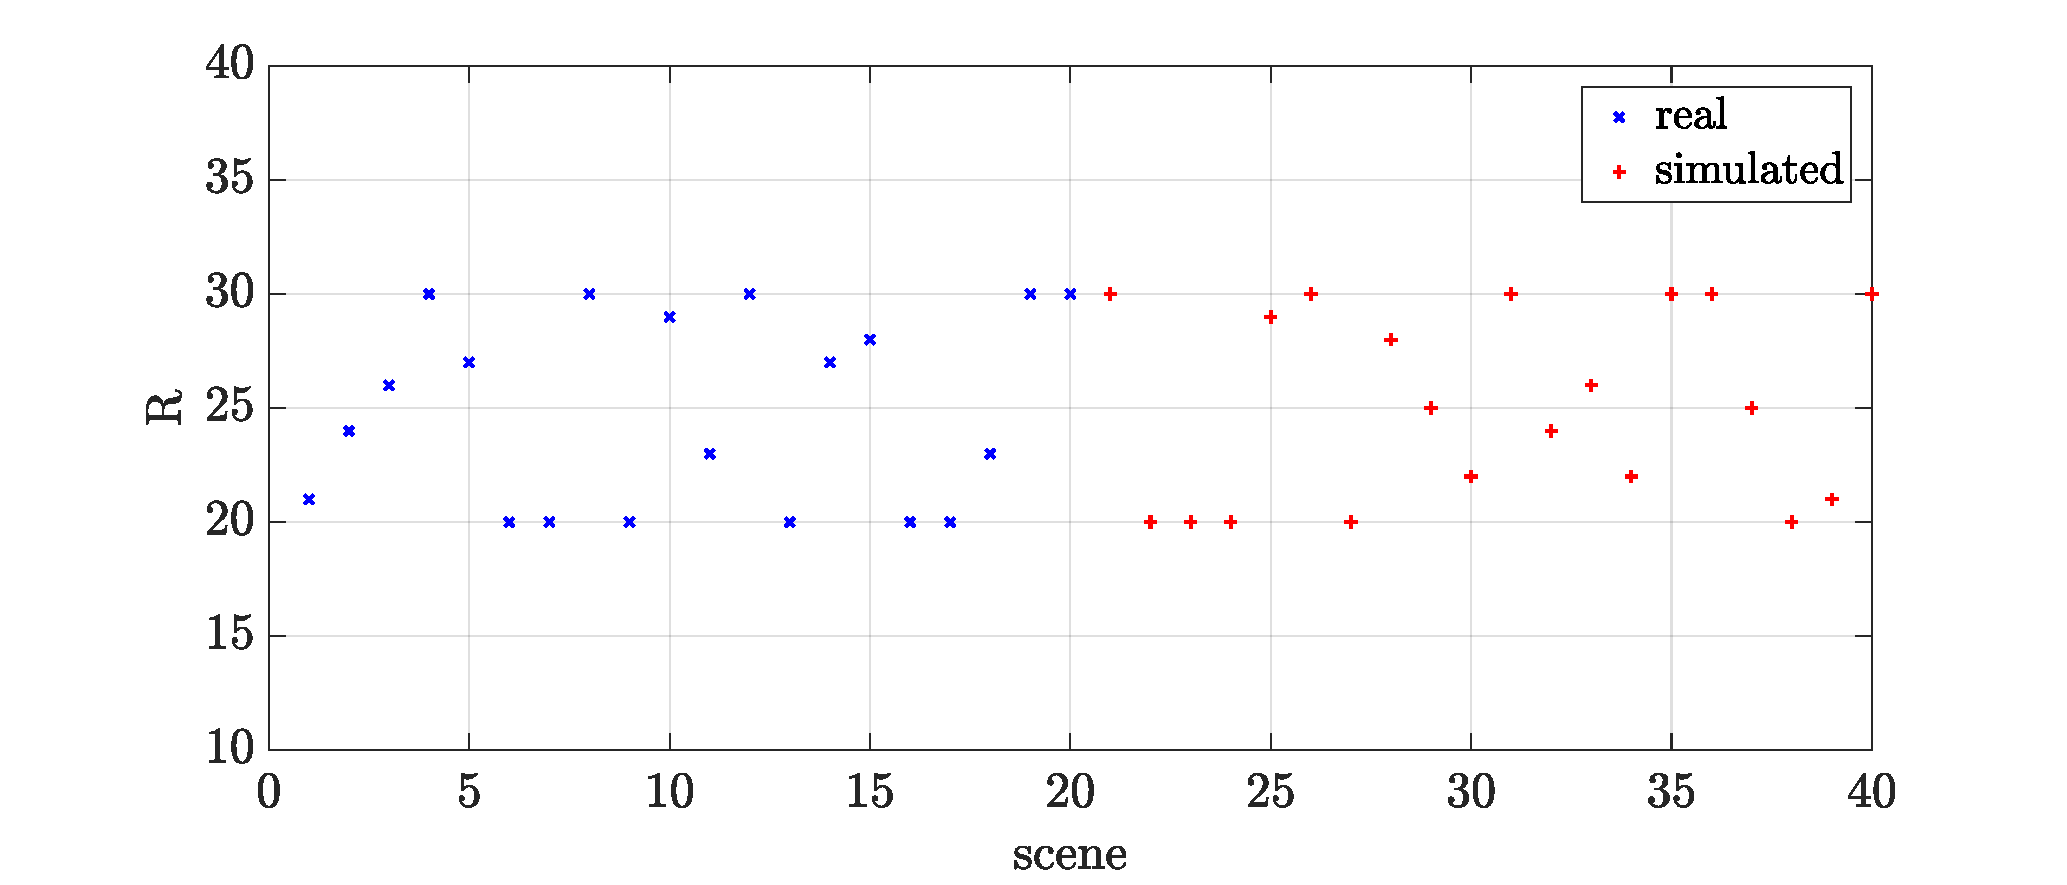
\includegraphics[width = 0.7\textwidth]{../../../Pictures/test_perceptif/nb_replication.pdf}
\caption{Nombre de réplication, $R$, pour chaque scène obtenu dans $X_{opt}$ avec comme combinaison $J = 50$, $B = 40$, $K = 20$. Les 20 premières scènes sont les scènes issus des enregistrements du projet GRAFIC, les 20 suivantes sont les scènes répliquées sous \textit{SimScene}.}
\label{fig:replication}
\end{figure}

L'optimisation du plan ne permet alors pas d'avoir un nombre de réplication $R$ constant mais variable évoluant dans l'intervalle $\left[20-30 \right]$. Toutefois, en moyenne, les scènes réelles et simulées sont écouté un même nombre de fois (25 fois). On s'assure ensuite que la répartition entre les scènes réels et simulées pour chaque juge est équitablement répartie (figure~\ref{fig:repartition}).\\

\begin{figure}[ht]
\centering
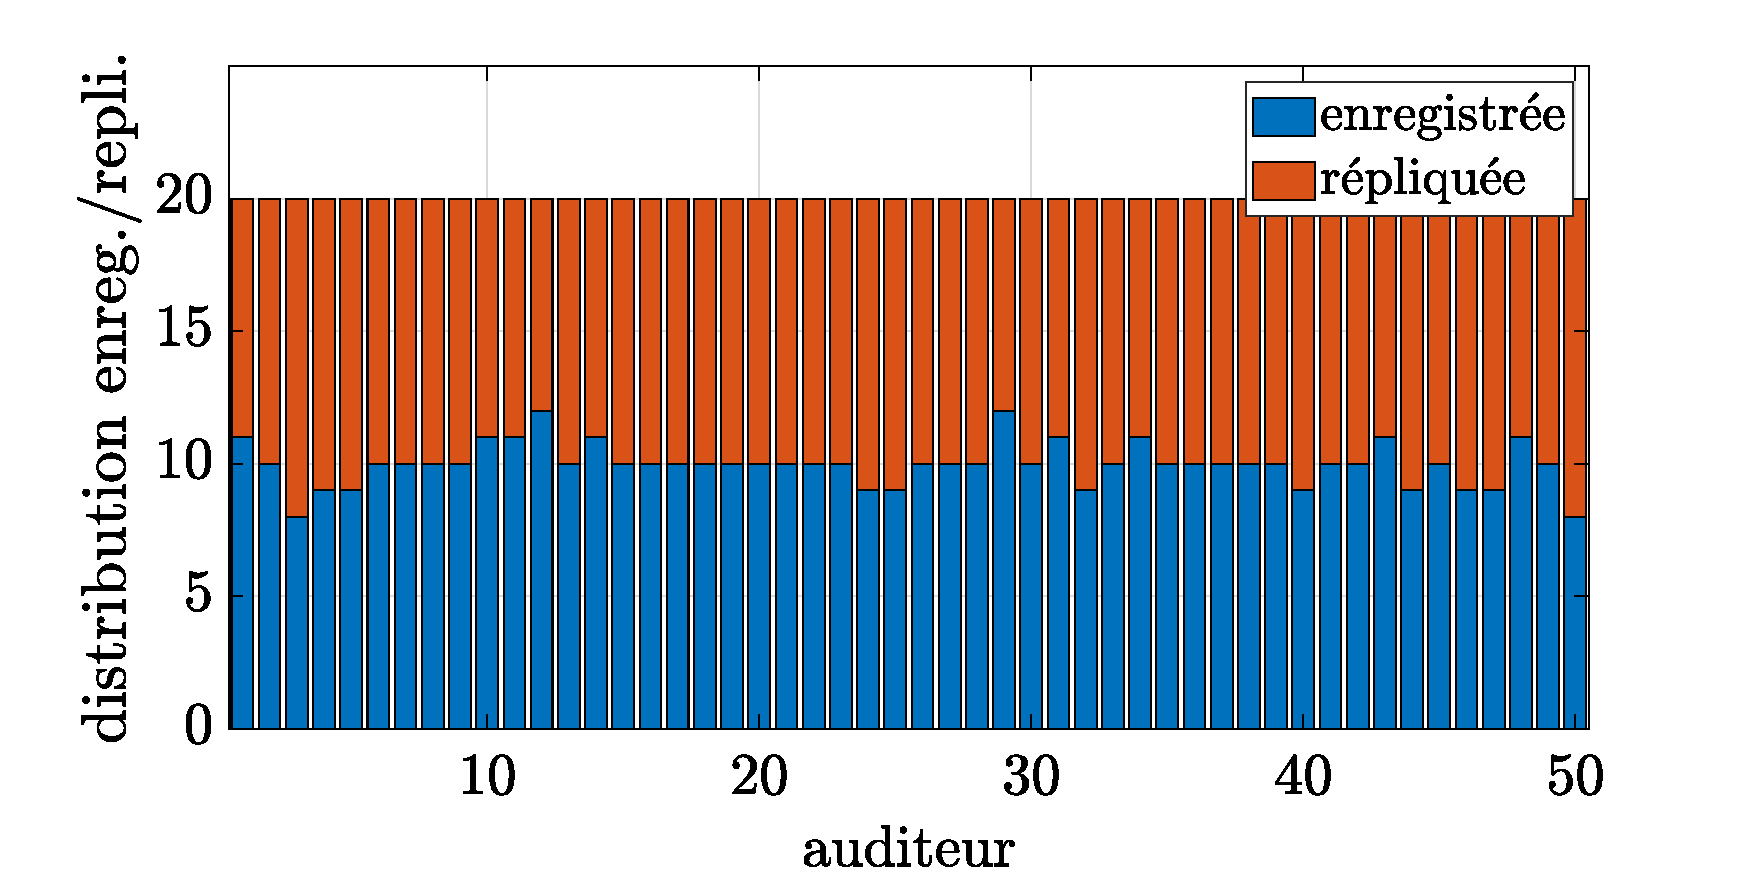
\includegraphics[width = .7\textwidth]{../../../Pictures/test_perceptif/repartition-real-simulated.pdf}
\caption{Répartition entre les scènes réelles et simulées par juge. La somme cumulée des deux ensembles correspond aux nombres d'écoutes $K$ qu'effectue un juge.}
\label{fig:repartition}
\end{figure}

Le plan généré permet bien d'avoir en moyenne une répartition équilibrée entre les scènes réelles et simulées, même si certain juges ont jusqu'à 12 scènes d'un même type.\\

Une page web \footnote{http://soundthings.org/research/xpRealism} est mis en ligne le 8 février 2017 permettant l'accès au test à une large public et s'est clôturé 12 jours plus tard. Chaque juge écoute donc une succession de 20 audio de 30 secondes dans un ordre établit par le plan optimal. Chaque audio peut être réécouter autant de fois que possible avant d'être évaluer sans qu'il soit toutefois possible de revenir sur son évaluation. L'auditeur a également la possibilité de laisser un commentaire sur chaque audio pour pouvoir justifier son choix. En fin de test, afin de connaitre le panel d'évaluateur, il est demandé aux juges de renseigner leur âge, leur sexe et leur expérience quant à l'écoute de mixtures sonores urbaines.\\

Les fichiers résultats sont stockés également sous une page web \footnote{http://soundthings.org/research/xpRealism/responses/} sous le format .json et sont traités sous le logiciel Matlab.\\

\subsection{Résultats}
\subsubsection{Constitution du panel}

La figure \ref{fig:panelTest} résume, sous forme d'histogrammes, l'âge, le sexe et l'expérience des auditeurs. 2 personnes ont renseigné aucun de ces champs et une troisième personne a seulement omis de préciser son sexe.\\

\begin{figure}[ht]
\centering
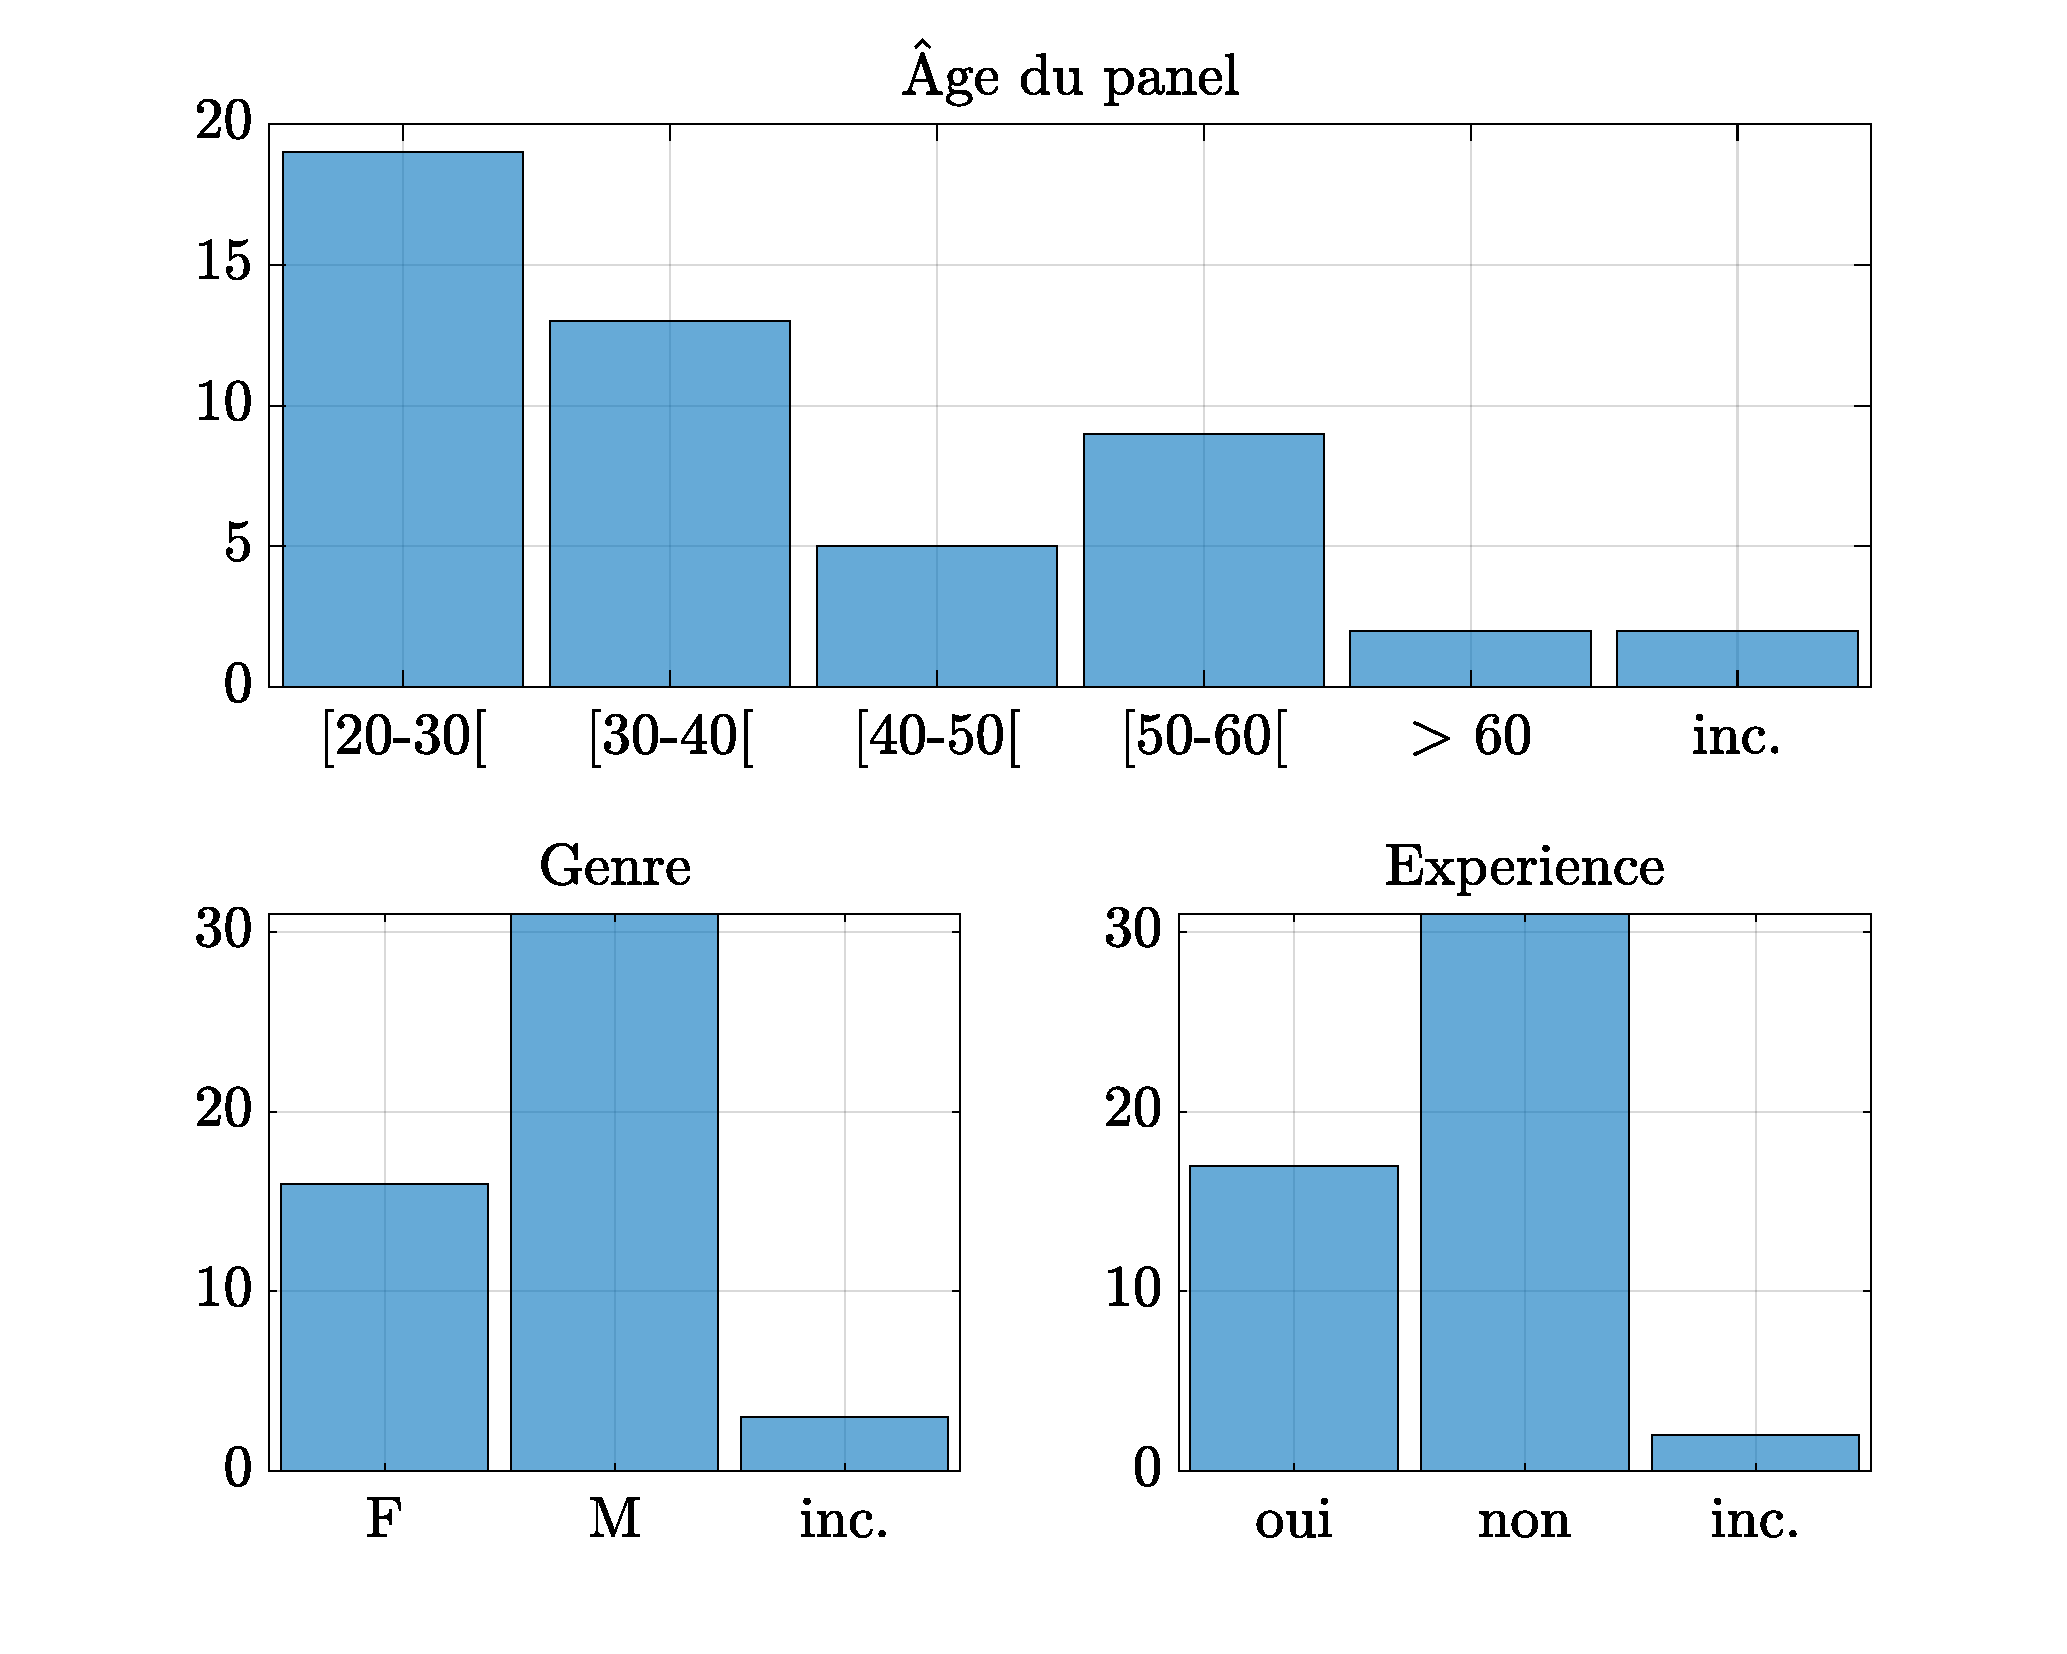
\includegraphics[width = .8\textwidth]{../../../Pictures/test_perceptif/testPerceptif_panel.pdf}
\caption{Résumé des informations relatifs aux panélistes}
\label{fig:panelTest}
\end{figure}

Le panel est composé à 62 $\%$ d'hommes et à 32 $\%$ de femmes. La classe d'âge $\left[20-30\right[$ est la plus représentée suivie de la classe $\left[30-40\right[$, 26 $\%$, $\left[50-60\right[$,  18 $\%$ $\left[40-50\right[$, $10\%$ et enfin de la classe $>60$,  4 $\%$ . 62 $\%$ du panel a déclaré n'avoir pas d'expérience dans l'écoute d'ambiances sonores urbaines contre 34 $\%$. Cette dernière caractéristique indique que la majorité des jugements provient d'auditeurs inexpérimentés dans ce domaine et se sont donc plus attardés sur une évaluation générale de la scène là où les auditeurs plus expérimentés se sont attardés en plus sur des aspects plus particulier comme la différence de réverbération entre les sources sonores. \\

\subsubsection{Modèle de l'ANOVA}
Une analyse de variance (abrégée ANOVA pour \textit{ANalyse Of VAriance} en anglais) est réalisée afin de savoir si la distribution des notes des scènes simulées (abrégé \textit{Si}) est similaire à celles de notes réelles (abrégé \textit{Re}) mais également pour connaitre l'influence de l'expérience de l'auditeur. N'ayant qu'une seule variable quantitative (les notes), c'est donc une ANOVA à 1 dimension qui est réalisée. Ce test statistique considère un nombre de facteur $F$ comprenant chacun un nombre $N$ de niveaux où $M_n$ observations sont réalisées dans chaque niveau. Le modèle s'exprime alors : 

\begin{equation}
y_{in} = \alpha_n + \epsilon_{in}
\end{equation}

où $y_{in}$  et $\alpha_k$ sont respectivement l'observation $i$ associé et l'effet moyen associé au niveau $j$ et $\epsilon_{in}$ est une erreur résiduelle suivant une loi normale centrée ($\epsilon_{in} \sim \mathcal{N}(0,\,\sigma^{2})$). Deux hypothèses sont alors émises sur les distributions : 

\begin{itemize}
\item les distributions des niveaux $n$ et $m$ sont semblables (hypothèse \textit{nulle} $H_0$),
\item les deux distributions sont différentes, (hypothèse \textit{alternative} $H_1$).\\
\end{itemize}

Le test statistique de Fischer détermine alors si l'hypothèse $H_0$ est vraie ou fausse (et donc si l'hypothèse $H_1$ est vérifiée). Ce test consiste à établir le rapport $\mathbf{F}$ de deux variances, 
 
\begin{equation}
\mathbf{F} = \frac{var_1}{var_2}.
\end{equation}

Le problème étant à 1 dimension, la variance totale $var_{tot}$ s'exprime comme la somme de la variance du modèle $var_{mod}$ (appelé variabilité inter-niveau) et celui d'un résidu $var_{res}$ (ou variabilité intra-niveau) : 

\begin{equation}
var_{tot} = var_{mod} + var_{res}.
\end{equation}

En considérant un nombre d'observation total $M = \sum_{k = 1}^{K} M_k$, chacune de ces variances s'exprime comme


\begin{equation}
var_{mod} = \frac{SCE_{mod}}{DDL_{mod}},
\end{equation}

\begin{equation}
var_{res} = \frac{SCE_{res}}{DDL_{res}} 
\end{equation}

avec 

\begin{itemize}
\item la somme des carrés des écarts du modèle, $SCE_{mod} = \sum_{n=1}^{N} m_n (\bar{y}_{in} - \bar{y})^2$, 
\item la somme des carrés des écarts du résidu, $SCE_{res} = \sum_{i=1}^{M_n} \sum_{n=1}^{N} (y_{in} - \bar{y}_n)^2$, 
\item le degré de liberté du modèle, $DDL_{mod} = F-1$,
\item le degré de liberté du résidu, $DDL_{res} = M-F$, 
\item $\bar{y} = $
\end{itemize}


Le rapport $\mathbf{F}$ s'exprime alors : 
\begin{align}
\mathbf{F} & = \frac{var_{mod}}{var_{res}}\\
& = \frac{\nicefrac{SCE_{mod}}{DDL_{mod}}}{\nicefrac{SCE_{res}}{DDL_{res}}}\\
& = \frac{M-F}{F-1}\frac{\sum_{n=1}^{N} m_n (\bar{y}_{in} - \bar{y})^2}{\sum_{i=1}^{M_n} \sum_{n=1}^{N} (y_{in} - \bar{y}_k)^2}.
\end{align}

Des degrés de libertés et de la valeur $\mathbf{F}$, on peut déterminer la \textit{p-valeur} (à l'aide des tables de Fischer ou à l'aide de logiciels comme \textit{R} ou Matlab) qui établit la probabilité d'obtenir une valeur limite du test si $H_0$ est vraie. Cette valeur est comparée a une seuil de signification $\alpha = 0.05$. Se présente alors deux cas :
 
\begin{itemize}
\item si $\alpha >$ \textit{p-valeur}, il existe alors au moins deux distributions différentes, l'hypothèse $H_0$ est rejetée et $H_1$ est acceptée,
\item si $\alpha <$ \textit{p-valeur}, l'hypothèse $H_0$ n'est pas considérée comme \textit{vraie} mais on considère alors qu'il n'y a pas de raison à rejeter $H_0$. Cette nuance provient du fait que cette décision se base sur un nombre limité d'informations (le nombre total d'observation $M$) qui ne permet pas de rejeter l'hypothèse $H_1$.\\
\end{itemize} 

\subsubsection{Par type de scènes}

Dans le cas du test perceptif, on considère un seul facteur ($F = 1$), le réalisme de la scènes, qui comprend deux niveaux \textit{réelles} et \textit{simulées} ($N = 2$), chaque niveaux ayant un nombre d'observation $M_n$ correspondant à l'ensemble des notes du panel appartenant à l'un des deux niveaux et un nombre totale d'individu $M = J \times K = 1000$. Une ANOVA est réalisée sous le logiciel Matlab et les résultats sont résumés dans le tableau \ref{tab:anova}.\\

\begin{table}[ht]
\centering
\begin{tabular}{lccccc}
\hline
\textbf{Source}     & \textbf{SCE} & \textbf{DDL} & \textbf{variance} & \textbf{F} & \textbf{p-valeur} \\
\hline
\textbf{réalisme} & 4.62         & 1            & 4.62              & 1.79       & 0.18              \\
\hline
\textbf{erreur}      & 2567.40      & 997          & 2.57              &            &                   \\
\hline
\textbf{total}      & 2572.00         & 998          &                   &            &       \\
\hline
\end{tabular}
\caption{Résultat de l'ANOVA calculé}
\label{tab:anova}
\end{table}


La \textit{p-valeur} est supérieure au seuil de signification $\alpha$ et est supérieur à 0.1. Il n'y a donc pas de présomption contre l'hypothèse $H_0$. On peut alors considéré qu'il n'y a pas de distinction possible entre les scènes simulées et réelles faites par le panel. \\

En plus des résultats textuels, une représentation graphique sous forme de diagramme en boîte à moustache est faite selon le type de scènes (figure \ref{fig:ANOVA_scene}). Cette représentation graphique permet de comparer plusieurs distributions en résumant pour chaque boîte la médiane (trait plein rouge), les valeurs du  premier quartile au troisième quartile (boîte en bleue), la valeur maximale et minimale de la distribution (respectivement trait supérieur et inférieur en noir). \`A cela est également ajoutée la moyenne.\\

%\begin{figure}[h]
%\centering
%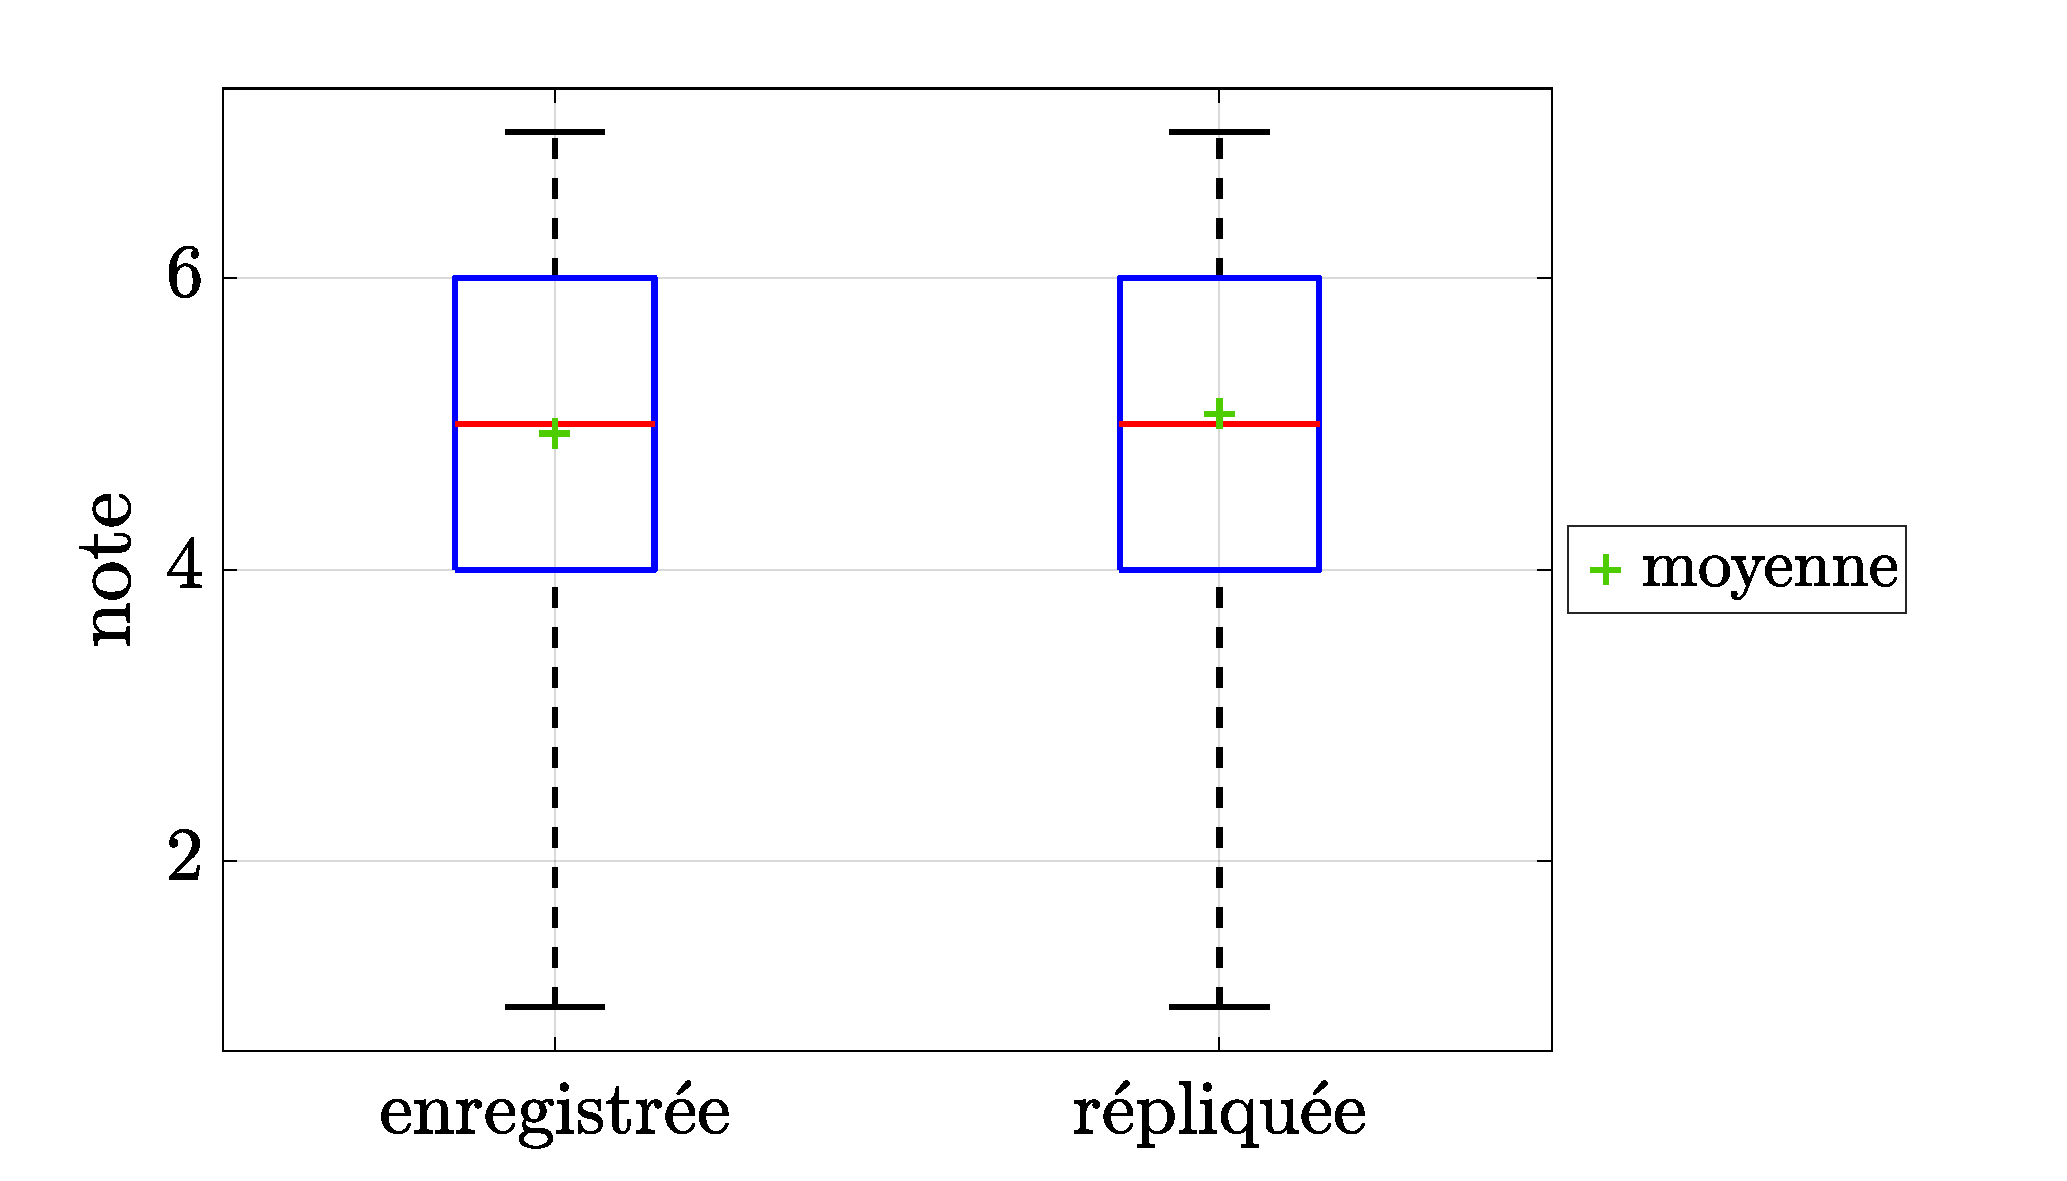
\includegraphics[width = 0.8\textwidth]{../../../Pictures/test_perceptif/testPerceptif_boxplotType.pdf}
%\caption{Représentation en diagramme en boîte à moustache entre les scènes réelles et simulées}\label{fig:ANOVA_scene}
%\end{figure}

La répartition des notes pour les deux type de scènes, quelque soit l'expérience de l'auditeur, est similaire. Chaque type présente des valeurs identiques (médiane, valeurs extrêmes, quantiles). Seule la note moyenne permet de différencier les deux ensembles : $m_{Re} = 4.93 \pm 1.64$ et $m_{Si} = 5.06 \pm 1.56$. Les deux valeurs sont quasiment similaires confirmant que les deux distributions sont donc bien identiques et que les scènes simulées ont un rendu similaire aux enregistrements réels. \\

\subsubsection{Par expérience et par type de scènes}
Il est possible de déterminer l'influence de l'expérience de l'auditeur dans les écoutes d'ambiances urbaines dans l'évaluation des scènes par un ANOVA (tableau~\ref{tab:anova_exp}, figure~\ref{fig:ANOVA_exp}). Il y a donc ici 2 facteurs $F$, le type de scènes et l'expérience, qui ont 2 niveaux $N$ chacun (respectivement Re/Si et expérience/sans expérience).

\begin{table}[ht]
\centering
\begin{tabular}{lccccc}
\hline
\textbf{Source}     & \textbf{SCE} & \textbf{DDL} & \textbf{variance} & \textbf{F} & \textbf{p-valeur} \\
\hline
\textbf{réalisme} & 4.62         & 1            & 4.62              & 1.79       & 0.18              \\
\hline
\textbf{expérience}    & 4.85         & 1            & 4.85              & 1.89       & 0.16              \\
\hline
\textbf{erreur}      & 2562.52      & 997          & 2.57              &            &                   \\
\hline
\textbf{total}      & 2572.00         & 999          &                   &            &       \\
\hline
\end{tabular}
\caption{Résultat de l'ANOVA calculé}
\label{tab:anova_exp}
\end{table}

%\begin{figure}[h]
%\centering
%\includegraphics[width = 0.8\textwidth]{../../../Pictures/test_perceptif/testPerceptif_boxplotExperience.pdf}
%\caption{Distribution des notes selon le type de scène et l'expérience dans l'écoute des scènes sonores urbaines}\label{fig:ANOVA_exp}
%\end{figure}


%\begin{table}[]
%\centering
%\begin{tabular}{p{3cm} C{3cm} C{3cm}}
%\cline{2-3}
% & \multicolumn{2}{c}{\textbf{type}} \\
%\cline{2-3}
% & \textbf{réelle} &  \textbf{simulée} \\ \hline
%\textbf{avec expérience} &  $5.13 \pm 1.60$ & $5.06 \pm 1.70 $ \\ \hline
%\textbf{sans expérience} &  $4.83 \pm 1.65$ & $5.07 \pm 1.49$ \\ \hline
%\end{tabular}
%\caption{Moyennes obtenue selon l'expérience et le type de scènes}
%\label{my-label}
%\end{table}

Si on différencie les auditeurs selon leur expérience dans l'écoute d'ambiances sonores urbaines, on constate que les auditeurs expérimentés évalue mieux les scènes réelles que les scènes simulées à l'inverse des auditeurs sans expériences. De plus, si les moyennes pour les scènes simulées sont fortement similaires quelque soit l'expérience, la notation des scènes réelles est différente. Des retours et remarques faites par plusieurs panéliste permette de supposer que les auditeurs plus expérimentés sont plus susceptibles de faire attention aux détails de la scènes (composition des évènements sonores, connaissance sur la panel de sons pouvant être présents, différence de réverbération entre les sources sonores..) rendant les scènes simulées plus identifiables. À l'opposé, les auditeurs non expérimentés vont plus s'attarder à évaluer l'ensemble de la scène. Or comme les scènes simulées sont constitué de sons qui sons isolés initialement, il est plus facile pour l'auditeur de les reconnaitre dans la scène qu'il écoute et donc de se \og  projeter \fg{} dans le milieu urbain. Dans certaines scènes réelles, les sources sonores étant moins discernables la perception du réalisme est réduite.\\

Toutefois, malgré ces faibles différences, les moyennes et les distributions restent, là encore, similaires et permettent de conclure que même avec de l'expérience dans l'écoute de scènes urbaine, la qualité des audio simulées est satisfaisante.\\

\subsubsection{Par ambiance et par scène}

On regroupe, dans la figure~\ref{fig:boxplot_ambiance}, les scènes par ambiances sonores (\textit{parc}, rue \textit{calme}, rue \textit{animée}, rue \textit{très animée}).\\

%\begin{figure}[hbtp]
%\centering
%\includegraphics[width=0.7\textwidth]{../../../Pictures/test_perceptif/testPerceptif_boxplotAmbianceCOLOR.pdf}
%
%\begin{tabular}{|p{1.5cm}|l|p{0.001cm}|p{2cm}|l|p{0.001cm}|p{2cm}|l|p{0.001cm}|p{2.75cm}|l|}
%\hhline{|-|-|~|-|-|~|-|-|~|-|-|}
%Parc & {\cellcolor[HTML]{5AB25A}} & & Rue calme & {\cellcolor[HTML]{FFCB2F}} & & Rue animée & {\cellcolor[HTML]{F56B00}} & &  Rue très animée & {\cellcolor[HTML]{9A0000}}\\
%\hhline{|-|-|~|-|-|~|-|-|~|-|-|}
%\end{tabular}
%
%\caption{Distribution en fonction de l'ambiance sonore pour les scènes réelles (en haut) et les scènes simulées (en bas)}
%\label{fig:boxplot_ambiance}
%\end{figure}

 
Cette représentation permet de constater que les ambiances sonores \textit{animée} et \textit{très animée}, dans les deux types de scènes, sont évaluées comme les plus réalistes : la médiane et la moyenne sont élevées avec une distribution peu dispersée. \`A l'inverse, les ambiances plus calmes (\textit{parc} et \textit{calme}) sont plus dispersés et ont une note moyenne plus faible. C'est donc les ambiances constituées en majorité du trafic qui sont les mieux évalués. Les scènes dans les parcs et rues calmes, constituées de moins de trafic et plus de sons urbains divers (voix, bruit de pas, oiseaux), sont moins bien évaluées aussi bien pour les scènes issus d'enregistrements que celles créer.\\

Enfin, pour chaque scène, la distribution des notes est établie et sont mis en relation avec les commentaires laissés par les auditeurs (figure~\ref{fig:ANOVA_scene}).\\

%\begin{figure}[h]
%\centering
%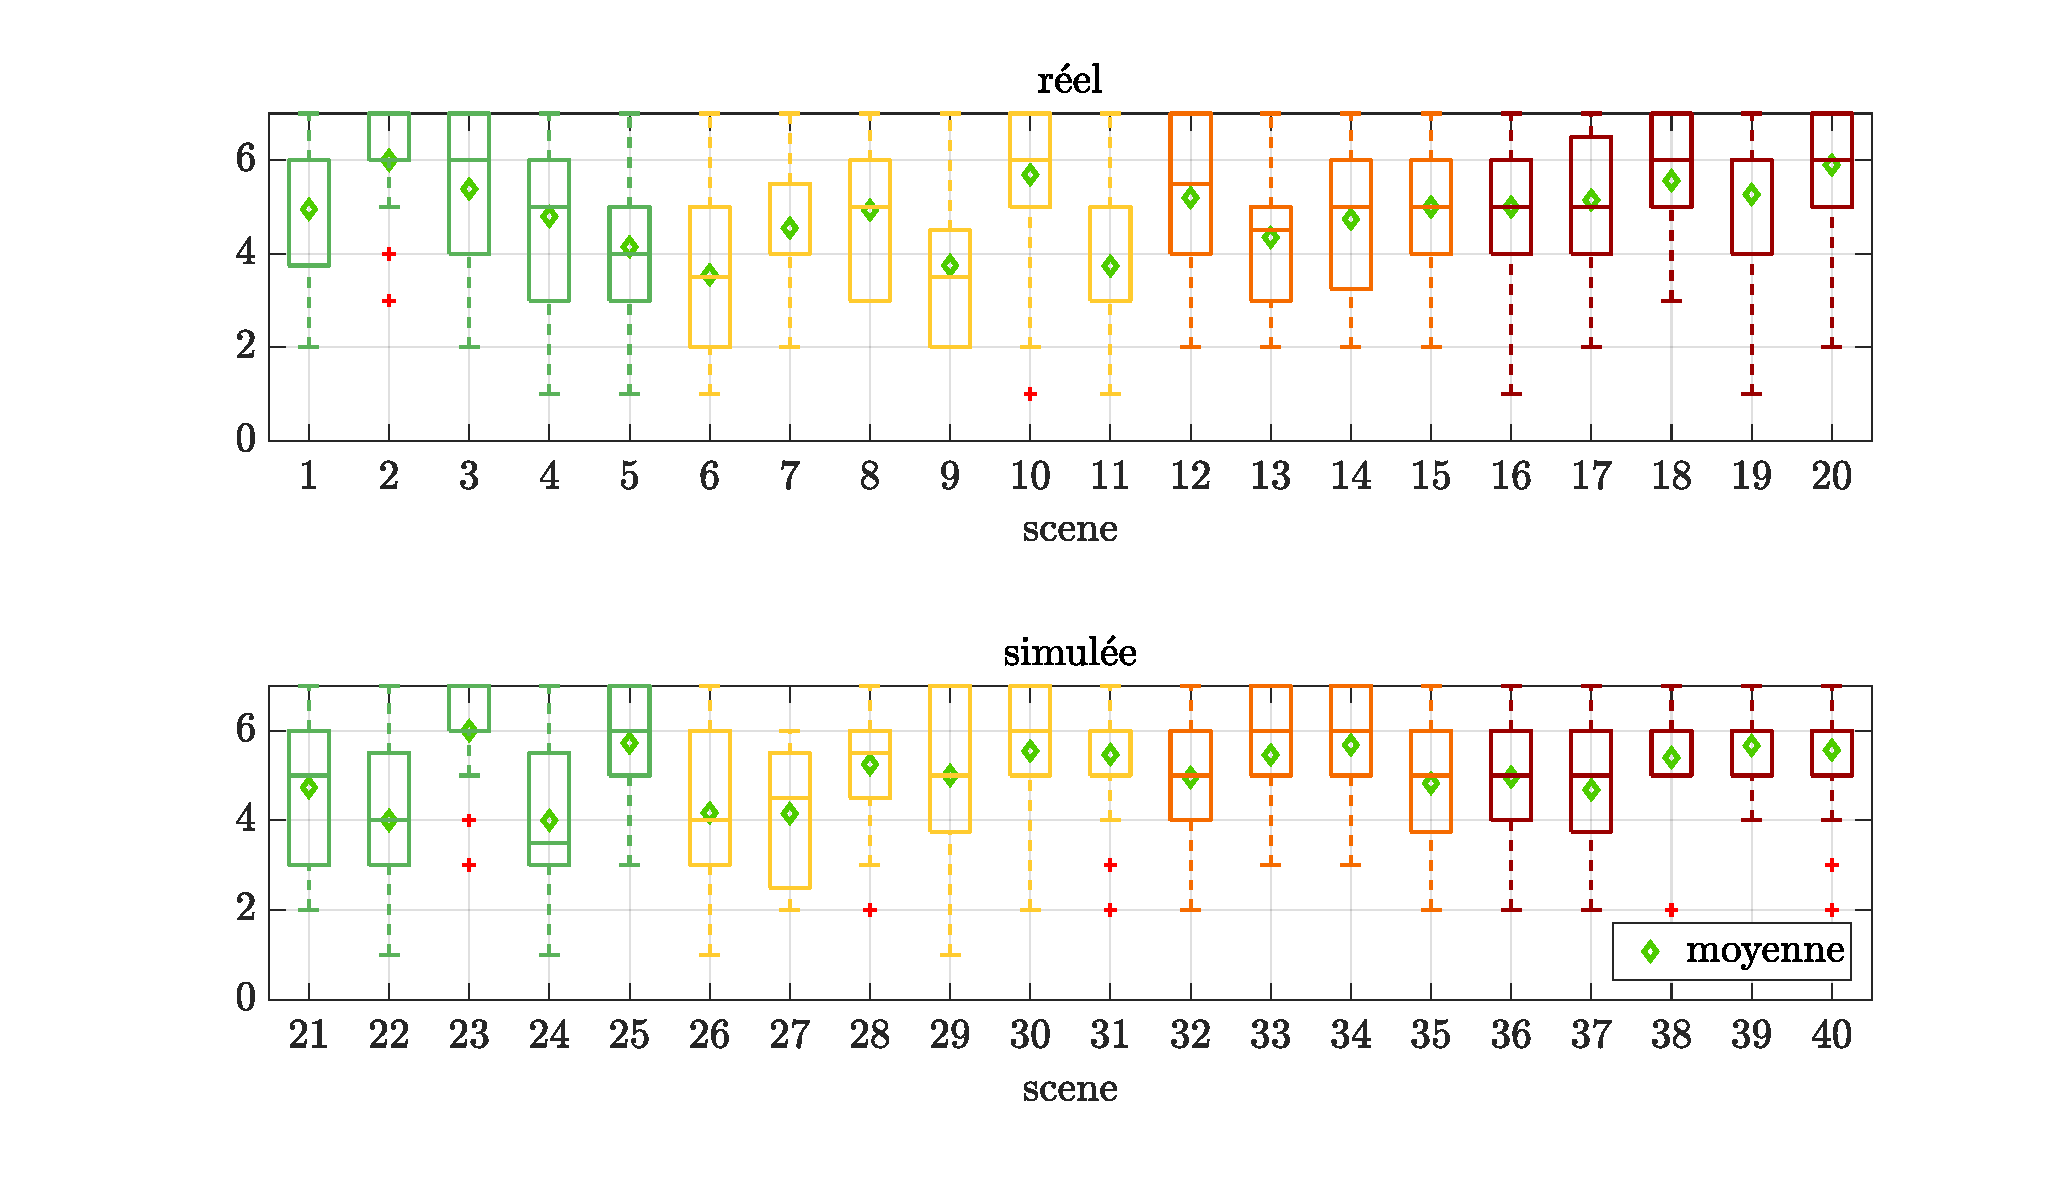
\includegraphics[width = .9\textwidth]{../../../Pictures/test_perceptif/testPerceptif_meanPerSceneCOLOR.pdf}
%
%\begin{tabular}{|p{1.5cm}|l|p{0.001cm}|p{2cm}|l|p{0.001cm}|p{2cm}|l|p{0.001cm}|p{2.75cm}|l|}
%\hhline{|-|-|~|-|-|~|-|-|~|-|-|}
%Parc & {\cellcolor[HTML]{5AB25A}} & & Rue calme & {\cellcolor[HTML]{FFCB2F}} & & Rue animée & {\cellcolor[HTML]{F56B00}} & &  Rue très animée & {\cellcolor[HTML]{9A0000}}\\
%\hhline{|-|-|~|-|-|~|-|-|~|-|-|}
%\end{tabular}
%
%\caption{Distribution par scène pour les scènes réelles (de 1 à 20) et les scènes simulées (de 21 à 40)}
%\label{fig:moyParScene}
%\end{figure}


Plusieurs observations peuvent être émises : 
\begin{itemize}
\item La meilleure moyenne est obtenue pour 2 scènes ex-æquo : la scène 2 (6.0 $\pm$ 1.0) et 23 (6.0 $\pm$ 1.1).
\item La plus mauvaise moyenne est réalisée pour la scène 6 (3.6 $\pm$ 1.6). C'est donc une scène issu d'un enregistrement qui a été jugé la moins réaliste. Celle-ci a la particularité de n'avoir aucun évènement sonore discernable. 
\item Parmi les 20 scènes simulées, on peut observé 4 scènes dont les moyennes sont plus faibles que les autres (scènes 22, 24, 26 et 27). Dans les scènes 24 et 26, les auditeurs ont remarqué que la présence des bruits de pas paraissent trop fort cassant le réalisme du reste de la scène. La scène 22 est, quant à elle, évaluée plus faiblement en raison d'un bruit de portail également trop fort au début de l'extrait. Ces trois scènes appartiennent à l'ambiance \textit{Parc}. La scène 27 enfin n'a pas reçu de commentaire mais sa note moyenne plus faible peut s'expliquer par un bruit de fond composé d'un nombre d'oiseaux peut être trop grand et qui parait peu réaliste dans un milieu urbain.\\
\end{itemize}

L'ensemble de cette étude met en évidence les performances de l'outil de simulation qui permet de reconstruire des mixtures sonores urbaines perçues comme suffisamment réalistes. Pour ce test, la réalisation des scènes aux ambiances rue \textit{animée} et \textit{très animée} est très correcte. Les ambiances \textit{parc} et rue \textit{calme} restent bien évalué sur leur réalisme mais sont perfectibles notamment sur certains évènements sonores, non reliés au trafic, qui détériore l'aspect réaliste des scènes. A noter, que les passages de voitures isolés ou la reconstitution du trafic n'ont pas fait l'objet de commentaire.

%\bibliographystyle{unsrt}
%\bibliography{../bibliographie}
%
%\end{document}

\chapter{\'Etude du comportement de la NMF sur le corpus d'évaluation \textit{ambiance}}
\label{chap:ambiance}

\section*{\centering Résumé}

\noindent{\small \textbf{
La NMF est appliquée sur le corpus d'évaluation \textit{Ambiance} afin de visualiser le comportement de cette méthode sur de telles mixtures sonores. Les trois méthodes retenues (NMF supervisée, semi-supervisée et initialisée seuillée) sont testées pour de multiples configurations selon la composition du dictionnaire et de la $\beta$-divergence. Les résultats obtenus permettent de constater des performances variables des méthodes selon la prédominance du trafic. Lorsque celui-ci est faible, la NMF semi-supervisée se révèle l'approche la plus performante alors que la NMF supervisée génère de plus faibles erreurs quand le trafic est la source sonore principale. La NMF IS est alors la méthode qui offre le meilleur compromis dans son fonctionnement grâce à la mise à jour de son dictionnaire et à l'estimation du signal \textit{trafic} par une méthode de seuillage dur.}}

\vspace{2cm}

Dans ce chapitre, on étudie le comportement des différentes versions de la NMF, présentées dans le chapitre \ref{chap:NMF},  avec le premier corpus élémentaire \textit{Ambiance}. Ce corpus présente l'intérêt d'être construit en mixant des classes de sons spécifiques dont la source sonore \textit{trafic} est calibrée à différents niveaux sonores. Cet aspect permet d'étudier le fonctionnement des différentes versions de la NMF en fonction de la prédominance du trafic et de la nature des classes de sons, ainsi que de déterminer les approches les plus efficaces et les plus adaptées à ces environnements.
Dans un premier temps un rappel du corpus, des méthodes choisies et une présentation de la méthode de référence (ou \textit{baseline} en anglais) sont exposés. Puis les étapes menant à l'apprentissage du dictionnaire et l'ensemble des facteurs expérimentaux sont détaillées. Enfin les résultats des calculs menés sont présentés et discutés.


\section{Rappel de la méthode employée}

Les étapes impliquées dans l'estimation du niveau sonore du trafic à partir de scènes sonores simulées sont d'abord rappelées. La Figure \ref{fig:rappel_estimateur} résume la démarche générale.

\begin{figure}[ht]
\centering
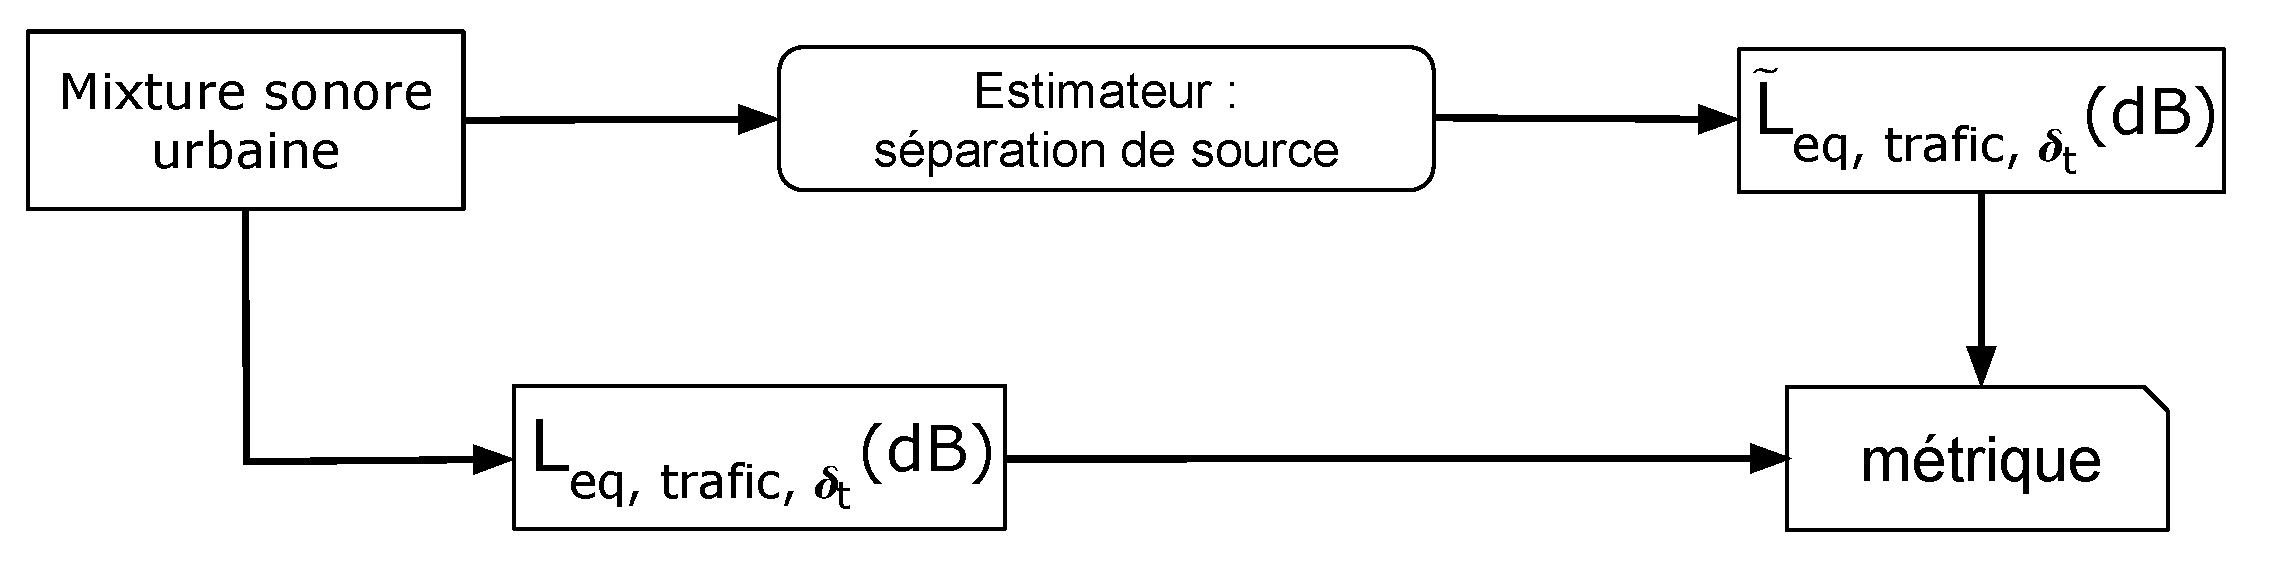
\includegraphics[width=.8\linewidth]{./figures/NMF/Bloc_diagram_estimateur_FR.pdf}
\caption{Schéma-bloc de l'estimation du niveau sonore du bruit de trafic.}
\label{fig:rappel_estimateur}
\end{figure}

Le corpus de scènes sonores, présenté dans \ref{part:corpus_ambiance}, est composé, pour rappel, de 6 sous-corpus : \textit{alerte}, \textit{animaux}, \textit{climat}, \textit{humain}, \textit{transport}, \textit{mécanique} (abrégés respectivement \textit{al.}, \textit{an.}, \textit{cl.}, \textit{hu.}, \textit{tr.} \textit{me.}). Chaque sous-corpus est lui-même divisé en 5 sous-ensembles qui comprennent, chacun, 25 mixtures sonores $M_i$ de 30 secondes, comprenant une classe de son \textit{trafic} (qui inclut le bruit de fond routier ainsi que les évènements sonores \textit{passages de voitures}), $S_{tr.}$, et une classe de son \textit{interférante} (qui regroupe tous les autres sources sonores), $S_{int.}$ :

\begin{equation}
M_i = S_{tr.,i}+S_{int.,i}.
\end{equation}

Dans chacun des 5 sous-ensembles sous-ensemble, le niveau sonore du signal \textit{trafic}, $L_{eq,tr.}$ est calibré par rapport au niveau sonore de la classe de son \textit{interférante}, $L_{eq,int.}$ tel que :

\begin{equation}
TIR = L_{eq,tr.} - L_{eq,int.}
\end{equation}

avec 5 valeurs $TIR \in \lbrace -12,~-6,~0,~6,~12 \rbrace$ dB. Ce corpus permet de tester les performances de la NMF et son comportement face à différentes sources sonores avec une prédominance variable du trafic routier. En tout, le corpus est composé de 750 scènes (6 sous-corpus $\times$ 5 $TIR$ $\times$ 25 scènes) pour une durée totale de 6h30.

Pour chaque $TIR$ et chaque sous-corpus, les 25 scènes $i$ sont soumises à un estimateur qui détermine le niveau sonore \textit{trafic} de l'intégralité de la scène en dB,  $\tilde{L}_{eq,tr., i}$. Les 25 niveaux sonores sont ensuite comparés aux niveaux sonores exacts respectifs, $L_{eq,tr., i}$ au travers de la métrique $MAE$ (équation \ref{eq:mae}), définie dans la partie \ref{sect:methode}. Il est ensuite possible de déterminer les performances d'un estimateur sur l'ensemble des 6 sous-corpus pour chaque $TIR$ en calculant sa moyenne :

\begin{equation}\label{eq:mae_tir}
MAE_{TIR} = \frac{\sum_{i = 1}^6 MAE_{i}}{6}.
\end{equation}

Il est enfin possible de calculer une erreur globale sur l'intégralité du corpus \textit{Ambiance}  :

\begin{equation}\label{eq:mae_g}
MAE_{g} = \frac{\sum_{i = 1}^6 \sum_{j = 1}^5 MAE_{i,j}}{6 \times 5}.
\end{equation}

L'erreur $MAE_g$ traduit l'erreur moyenne de l'estimateur faite sur l'intégralité du corpus d'évaluation et donc celle qui serait faite si aucune connaissance \textit{a priori} sur l'environnement sonore n'était disponible.

\section{Estimateur baseline}
Dans un premier temps, un estimateur de référence (ou \textit{baseline} en anglais) est nécessaire afin de comparer les performances de la NMF. La baseline choisie est un filtre passe-bas de fréquence de coupure $f_c$. L'hypothèse faite est que l'énergie située dans la bande passante est assimilable au signal \textit{trafic}, $\tilde{L}_{eq,trafic}$. Le choix de cet outil est justifié par la présence de composantes basses-fréquences (principalement en dessous de 1000 Hz) dans les signaux trafic. Supprimer l'énergie au-delà parait donc une première approche envisageable. %De plus, c'est une méthode qui pourrait être choisie par défaut.
Cet estimateur consiste à représenter une mixture $M_i$ sous la forme d'un spectrogramme puis à rejeter toutes les trames fréquentielles supérieures à $f_c$. La Figure \ref{fig:baseline} résume les étapes intervenant pour cet estimateur.

\begin{figure}[hbtp]
\centering
\includegraphics[width=\linewidth]{./figures/NMF/filtre_principe.pdf}
\caption{Principe de l'estimateur \textit{baseline}  pour une mixture sonore filtrée à $f_c$ = 5kHz.}
\label{fig:baseline}
\end{figure}

Les fréquences de coupure choisies sont $f_c \in \lbrace 100, 500, 1k, 2k, 5k, 10k, 20k \rbrace$ Hz. Le cas où $f_c = 20$ kHz correspond finalement au cas où aucun traitement du signal n'est réalisé sur les fichiers audio et où toutes les sources présentes sont assimilées au trafic, ce qui correspond à l'utilisation actuellement faite des mesures pour la correction de cartes de bruits issues de modèles prédictifs.

%\ml{je viens de lire sur la mesure d'impact des éoliennes, et ils utilisent des termes comme niveau ambient, résiduel ou d'émergence, ce serait peut etre approprié des les utiliser.}

\section{Estimateur basé sur la NMF}
Le second estimateur est celui basé sur la NMF, présentée dans le chapitre \ref{chap:NMF}. Pour rappel, cette méthode consiste à approximer le spectrogramme $\mathbf{V}$ d'un signal audio par le produit de deux matrices, $\mathbf{W}$, un dictionnaire de spectres sonores, et $\mathbf{H}$, une matrice d'activation temporelle. La Figure \ref{fig:nmf_ambiance} rappelle les différentes étapes présentes dans cet estimateur.

\begin{figure}[ht]
\centering
\includegraphics[width=0.7\linewidth]{./figures/NMF/NMF_ambiance.pdf}
\caption{Diagramme en blocs de l'estimateur NMF sur le corpus d'évaluation \textit{Ambiance}.}
\label{fig:nmf_ambiance}
\end{figure}


\subsection{Constitution du dictionnaire} 

Dans un premier temps, le dictionnaire $\mathbf{W}$ est construit, à partir d'un corpus d'apprentissage composé de 53  enregistrements audio des passages des voitures Renault Scénic et Dacia Sandero. Ces enregistrements ont été réalisés sur la piste d'essais de l'Ifsttar dans les mêmes conditions d'enregistrements que les 2 véhicules composants le corpus élémentaire de \textit{SimScene} (voir partie \ref{part:voiture_record}). Ces 53 échantillons audio issus des enregistrements ne sont pas ceux utilisés dans la création des scènes sonores afin d'éviter tout problème de sur-apprentissage.

\begin{figure}[hbtp]
\centering
\includegraphics[width=.9\linewidth]{./figures/NMF/creation_dictionaire.pdf}
\caption{Diagramme en blocs de la création du dictionnaire.}
\label{fig:creation_W}
\end{figure}

La constitution du dictionnaire est réalisée en trois étapes, résumées dans le diagramme en blocs montré Figure \ref{fig:creation_W} :
\begin{itemize}
\item chaque fichier audio est représenté au travers d'un spectrogramme, obtenu par une Transformée de Fourier à Court Terme (nombre de point $w = 2^{12}$ avec 50 $\%$ de recouvrement). Cette première étape permet d'obtenir pour chaque échantillon audio, de durée différente, le même nombre de points en fréquences.
\item Chaque spectrogramme est ensuite découpé en plusieurs fenêtre temporelles de durée $w_t \in \lbrace 0.5,~ 1,~ 2\rbrace$ seconde(s). 
Dans chacune des fenêtres, la valeur efficace \textit{rms} sur chaque trame fréquentielle est calculée. Ce procédé, qui équivaut à un sous échantillonnage, a pour but d'obtenir différentes représentations des spectrogrammes initiaux avec une description du contenu spectral plus ou moins fine. Dans le cas où $w_t = 0,5$ s, les spectres sonores contiennent plus de détails que dans le cas où $w_t = 2$ s. Les étapes de ce processus sont résumées en Figure \ref{fig:decoupe_W} sur un extrait de 3 secondes.
\item Enfin, l'opération précédente générant un grand nombre d'éléments (2218 pour $w_t$ = 0,5 s, 505 pour $w_t$ = 2 s), une quantification vectorielle, opérée grâce à un algorithme de clustering $K$-means, est appliquée en vue de réduire ce nombre à $K = \lbrace 25,~50,~100,~200 \rbrace$ et d'éviter la présence d'informations redondantes. Les $K$ centroïdes obtenus par cet algorithme sont alors les éléments qui composent le dictionnaire $\mathbf{W}$.
\end{itemize}

En plus de ces étapes, on ajoute un cas où la valeur \textit{rms} est calculée sur l'ensemble des spectrogrammes ($w_t = all$). Des 53 fichiers audio du corpus d'apprentissage, 53 spectres sont générés. Cette opération permet de baser la construction du dictionnaire sur les enveloppes spectrales des fichiers audio \textit{trafic} et moins sur une description fine des spectres. Ces 53 spectres sont également soumis à l'algorithme de clustering mais avec cette fois, $K_{w_t = all} \in \lbrace 25,~ 50 \rbrace$.
L'ensemble de ces facteurs expérimentaux et leurs modalités sont résumés dans le Tableau \ref{tab:experimental_factorsNMF_ambiance}. L'intérêt de ces paramètres est de multiplier le nombre de format que peut prendre le dictionnaire pour ainsi estimer l'influence de la forme des composantes et leur nombre dans l'estimation du niveau sonore du trafic selon les différentes NMF. Enfin, chaque élément du dictionnaire $\mathbf{w}$, pour toutes les combinaisons testées, est normalisé selon la norme $\ell_1$ telle que 
$\Vert \mathbf{w} \Vert_1 = \sum_{f = 1}^{F} w_f =  1$.

\begin{figure}[hbtp]
\centering
\includegraphics[width=\linewidth]{./figures/NMF/dictionaire_frame_FR.pdf}
\caption{Création des éléments de $\mathbf{W}$ sur un extrait de 3 secondes du passage d'une voiture pour une trame temporelle $w_t$ = 1 seconde. À gauche, le spectrogramme du signal audio avec, en pointillés, une fenêtre de découpe. Au centre, le signal découpé en trois trames et dont les valeurs \textit{rms} sont ensuite calculées générant 3 spectres.}
\label{fig:decoupe_W}
\end{figure}

\subsection{Réalisation de la NMF}

Chaque version du dictionnaire $\mathbf{W}$ est utilisé par l'estimateur du niveau de traffic. Cet estimateur est lui-même basé sur plusieurs versions de la NMF décrites précédemment (voir chapitre \ref{chap:NMF})  : la NMF supervisée (NMF SUP), semi-supervisée (NMF SEM) et initialisée-seuillée (NMF IS). Pour chaque NMF, 3 $\beta$-divergences sont utilisées : la distance Euclidienne ($\beta = 2$) (voir partie \ref{part:dist_EUC}, la divergence de Kullback-Leibler ($\beta = 1$) (partie \ref{part:div_KL}), et la divergence d'Itakura-Saïto ($\beta = 0$) (partie \ref{part:div_IS}). La NMF SUP dépend seulement des différentes versions du dictionnaire apprises et des valeurs de $\beta$. Le signal trafic est estimé selon l'équation \ref{eq:WH_trafic} à partir de la matrice $\mathbf{H}$ obtenue.
Dans le cas de la NMF SEM, le dictionnaire appris compose la partie fixe $\mathbf{W_s}$. Le nombre d'éléments du dictionnaire libre $\mathbf{W_r}$ est alors fixé à 2 ($J = 2$). Le signal \textit{trafic} est ensuite déterminé par le relation \ref{eq:WSHs_trafic}.
Enfin pour la NMF IS, les dictionnaires appris correspondent aux dictionnaires initiaux $\mathbf{W_0}$ qui seront ensuite mis à jour. À chaque itération, les éléments du dictionnaire sont également tous normalisés. Les dictionnaires obtenus $\mathbf{W'}$ sont ensuite soumis à l'étape d'extraction par seuillage qui implique également plusieurs facteurs expérimentaux :

\begin{itemize}
\item la représentation de la distance entre les dictionnaires initiaux et finaux $D_{\theta}(\mathbf{W_0} \Vert \mathbf{W'})$ (linéaire ou bien exprimé au travers d'une fonction sigmoïde ($\lambda = 2$)),
\item le type de seuillage appliqué (dur ou \textit{firm}),
\item les valeurs des différents seuils respectifs ($t_h$ pour le seuillage dur et $t_{f,1/2}$, les deux valeurs seuils pour le seuillage \textit{firm}). Des études préliminaires ont permis de réduire la plage des valeurs de ces seuils à $t_h \in \left[ 0,30~0,70 \right]$, $t_{f,1} \in \left[ 0,20~0,55 \right]$ et $t_{f,2} \in \left[ 0,35,~0,70 \right]$, chacun étant défini avec un pas de 0,01. Rappelons que pour le seuillage \textit{firm}, $t_{f,1} \leq t_{f,2}$.
\end{itemize}

Malgré la réduction du nombre d'éléments par l'algorithme $K$-means, la taille des matrices $\mathbf{W}$ et $\mathbf{V}$ reste importante en raison du nombre de trames fréquentielles ($F$ = 2049). En conséquence, ces deux matrices sont exprimées en bandes de tiers-d'octaves ce qui réduit les dimensions des matrices ($F_{1/3} = 29$). L'allure d'un spectre du passage d'une voiture en bandes fines et en tiers d'octaves est représenté en Figure \ref{fig:tiers_octaves}. La manipulation des matrices est alors plus rapide qu'avec les bandes fines et permet donc un gain en temps de calcul. Cette représentation a également d'autres intérêts :

\begin{itemize}
\item par son échelle logarithmique, elle décompose mieux les basses fréquences que les hautes fréquences ce qui permet de mieux focaliser la reconstruction du signal vers les bandes de fréquences d'intérêt.
\item Cette représentation est également couramment utilisée dans le domaine de l'acoustique urbaine et environnementale, à la différence des MFCC. Notamment tous les réseaux de mesures en ville déterminent des valeurs du niveaux sonores en bande de tiers d'octave. Cela en fait donc une représentation adaptée.
\end{itemize}

\begin{figure}[h]
\centering
\includegraphics[width=0.5\linewidth]{./figures/NMF/bande_fine_tiers.pdf}
\caption{Spectre en fréquence du passage d'une voiture en bandes fines (2049 points) et en bandes de tiers d'octave (29 bandes).}
\label{fig:tiers_octaves}
\end{figure}

Enfin, le nombre d'itérations est fixé à 100 pour toutes les versions de la NMF étudiées.

\subsection{Résumé des facteurs expérimentaux}

De nombreux facteurs expérimentaux sont donc présents dans cette expérience, chacun ayant différentes modalités. Le Tableau \ref{tab:experimental_factorsNMF_ambiance} résume l'ensemble de ces paramètres dont les différents sous-corpus, valeurs du $TIR$ et facteurs expérimentaux liés aux estimateurs. La Figure \ref{fig:organigramme} représente les différents facteurs expérimentaux impliqués dans l'estimateur ainsi que leurs liens de dépendances.

\begin{figure}[h]
\centering
\includegraphics[width=0.8\linewidth]{./figures/NMF/facteurs_exp.pdf}
\caption{Organigramme des différents facteurs expérimentaux impliqués dans l'outil \textit{estimateur}.}
\label{fig:organigramme}
\end{figure}

\begin{table*}[h]
\centering
\caption{Facteurs expérimentaux et leurs modalités utilisés pour le corpus d'évaluation \textit{Ambiance}.}
\begin{tabularx}{17.5cm}{L{3cm}@{}C{12cm}@{}C{2cm}@{}}
	\hline
    \textbf{\begin{tabular}[c]{@{}l@{}}facteurs \\ expérimentaux \end{tabular}} & \textbf{modalités} & \begin{tabular}[c]{@{}C{2cm}@{}}\textbf{nombre de}\\ \textbf{modalités}\end{tabular}\\ \toprule
\end{tabularx}

\begin{tabularx}{17.5cm}{L{2.8cm}@{}@{}C{2cm}@{}@{}C{2cm}@{}@{}C{2cm}@{}@{}C{2cm}@{}@{}C{2cm}@{}@{}C{2.2cm}@{}C{2cm}}
   \textbf{sous-corpus} & alerte (al.) & animaux (an). & climat (cl.) &  humain (hu.) & transport (tr.) & mécanique (me.) & 6\\
\end{tabularx}

\begin{tabularx}{17.5cm}{L{2.8cm}@{}@{}C{2.435cm}@{}@{}C{2.435cm}@{}@{}C{2.435cm}@{}@{}C{2.435cm}@{}@{}C{2.435cm}@{}C{2cm}}
\rowcolor[HTML]{C0C0C0}
   $TIR$ (dB) & -12 & -6 & 0 & 6 & 12 & 5\\
\end{tabularx}

\begin{tabularx}{17.5cm}{L{3cm}@{}C{3cm}@{}@{}C{3cm}@{}@{}C{3cm}@{}@{}C{3cm}@{}C{2cm}@{}}
  \textbf{estimateur} & filtre passe bas & NMF SUP & NMF SEM & NMF IS & 4\\
\end{tabularx}

\begin{tabularx}{17.5cm}{L{3cm}@{}@{}C{1.71cm}@{}@{}C{1.71cm}@{}@{}C{1.71cm}@{}@{}C{1.71cm}@{}@{}C{1.71cm}@{}@{}C{1.71cm}@{}@{}C{1.71cm}@{}C{2cm}@{}}
\rowcolor[HTML]{C0C0C0}
   $f_c$ (kHz) & 0,1 & 0,5 & 1 & 2 &  5 & 10 & 20 & 7\\
\end{tabularx}

\begin{tabularx}{17.5cm}{L{3cm}@{}C{3cm}@{}@{}C{3cm}@{}@{}C{3cm}@{}@{}C{3cm}@{}C{2cm}@{}}
    $w_t$ (s)& 0,5 & 1 & 2 & \textit{all} & 4\\
\end{tabularx}

\begin{tabularx}{17.5cm}{L{3cm}@{}C{3cm}@{}@{}C{3cm}@{}@{}C{3cm}@{}@{}C{3cm}@{}C{2cm}@{}}
	\rowcolor[HTML]{C0C0C0}
    $K$ & 25 & 50 & 100 & 200 & 4\\
\end{tabularx}

\begin{tabularx}{17.5cm}{L{3cm}@{}C{4cm}@{}@{}C{4cm}@{}@{}C{4cm}@{}C{2cm}@{}}
   $\beta$ & 0 & 1 & 2 & 3\\
\end{tabularx}

\begin{tabularx}{17.5cm}{L{3cm}@{}C{6cm}@{}@{}C{6cm}@{}C{2cm}@{}}
	\rowcolor[HTML]{C0C0C0}
   \textbf{représentation} & linéaire & sigmoïde & 2\\
\end{tabularx}

\begin{tabularx}{17.5cm}{L{3cm}@{}C{6cm}@{}@{}C{6cm}@{}C{2cm}@{}}
   \textbf{seuillage} & dur & \textit{firm} & 2\\
\end{tabularx}

\begin{tabularx}{17.5cm}{L{3cm}@{}C{12cm}@{}C{2cm}@{}}
	\rowcolor[HTML]{C0C0C0}
	\textbf{seuil dur} $\mathbf{t_h}$ & de 0,30 à 0,60 avec un pas de 0.01 & 31\\
\end{tabularx}

\begin{tabularx}{17.5cm}{L{3cm}@{}C{12cm}@{}C{2cm}@{}}
   \textbf{seuil firm} $\mathbf{t_{f,1}}$ & de 0,20 à 0,55 avec un pas de 0,01 & 36\\
\end{tabularx}

\begin{tabularx}{17.5cm}{L{3cm}@{}C{12cm}@{}C{2cm}@{}}
	\rowcolor[HTML]{C0C0C0}
   \textbf{seuil firm} $\mathbf{t_{f,2}}$ & de 0,35 à 0,70 avec un pas de 0,01 & 36\\
   \bottomrule
\end{tabularx}
\label{tab:experimental_factorsNMF_ambiance}
\end{table*}

Pour l'estimateur filtre, c'est donc 210 combinaisons qui sont réalisées (6 sous-corpus $\times$ 5 $TIR$ $\times$ 7 $f_c$). Dans le cas de la NMF SUP et SEM, ce sont respectivement 1260 combinaisons qui sont évaluées (6 sous-corpus $\times$ 5 $TIR$ $\times$ (3 $w_t$ $\times$ 4 $K$ + 1 $w_t$ $\times$ 2 $K$ ) $\times$ 3 $\beta$). Dans le cas de la NMF IS, ce nombre est beaucoup plus élevé (2 789 640) en raison des nombreuses valeurs seuils (6 sous-corpus $\times$ 5 $TIR$ $\times$ (3 $w_t$ $\times$ 4 $K$ + 1 $w_t$ $\times$ 2 $K$ ) $\times$ 3 $\beta$ $\times$ 2 représentation $\times$ (31 + 1076)).

Les calculs exhaustifs de toutes les combinaisons expérimentales sont réalisés avec le logiciel Matlab à l'aide de l'outil expLanes\footnote{\url{http://mathieulagrange.github.io/expLanes}} qui permet la réalisation d'expériences numériques, de gérer la distribution des nombreux facteurs expérimentaux et leur modalités et de collecter les nombreux résultats générés. %L'ordinateur menant les calculs est équipé d'un processeur Intel Core i7 (CPU 2,40 GHz).

\section{Performances de l'estimateur \textit{baseline}}

Les résultats issus de l'estimateur \textit{baseline} sont d'abord présentés. Dans un premier temps, les erreurs $MAE_g$ (équation \ref{eq:mae_g}) générées par les estimations réalisées par chaque fréquence de coupure sont résumées dans le Tableau \ref{tab:resuls_ambiance_filtre} ainsi que les erreurs $MAE_{TIR}$.

\begin{table}[h]
\centering
\caption{Erreurs $MAE_g$ de l'estimateur \textit{baseline} selon $f_c$ sur l'ensemble du corpus \textit{Ambiance} et pour chaque $TIR$. En gras-rouge l'erreur $MAE_g$ la plus faible, en gras-noir, les erreurs $MAE_{TIR}$ les plus faibles selon les fréquences $f_c$.}
\label{tab:resuls_ambiance_filtre}
\resizebox{\textwidth}{!}{%
\begin{tabular}{lcccccc}
\toprule
$f_c$ (Hz) & $MAE_g$ & $MAE_{-12}$ & $MAE_{-6}$ & $MAE_{0}$ & $MAE_{6}$ & $MAE_{12}$ \\
\midrule
 100 & 3,21 ($\pm$ 1,06) & \textbf{4,55 ($\pm$ 1,55)} & \textbf{2,92 ($\pm$ 0,42)} & 2,36 ($\pm$ 0,71) & 2,97 ($\pm$ 0,41) & 3,25 ($\pm$ 0,32)\\
 \rowcolor[HTML]{C0C0C0}
 500 & \textbf{\textcolor{red}{2,89 ($\pm$ 2,84)}} & 7,39 ($\pm$ 3,00) & 3,44 ($\pm$ 1,65) & \textbf{1,17 ($\pm$ 0,24)} & 1,03 ($\pm$ 0,26) & 1,45 ($\pm$ 0,13) \\
 1000 & 3,36 ($\pm$ 3,63) & 9,44 ($\pm$ 2,03) & 4,78 ($\pm$ 1,34) & 1,62 ($\pm$ 0,54) & \textbf{0,36 ($\pm$ 0,10)} & 0,61 ($\pm$ 0,06) \\
 \rowcolor[HTML]{C0C0C0}
 2000 & 3,83 ($\pm$ 4,01) & 10,30 ($\pm$ 1,57) & 5,65 ($\pm$ 1,05) & 2,25 ($\pm$ 0,49) & 0,62 ($\pm$ 0,15) & \textbf{0,11 ($\pm$ 0,02)}\\
 5000 & 4,51 ($\pm$ 4,43) & 11,95 ($\pm$ 0,20) & 6,70 ($\pm$ 0,16) & 2,82 ($\pm$ 0,10)  & 0,87 ($\pm$ 0,04) & 0,20 ($\pm$ 0,02)\\
 \rowcolor[HTML]{C0C0C0}
10000 & 4,64 ($\pm$ 4,51) & 12,19 ($\pm$ 0,08) & 6,90 ($\pm$ 0,07) & 2,95 ($\pm$ 0,05) & 0,92 ($\pm$ 0,02) & 0,22 ($\pm$ 0,01)\\
20000 & 4,69 ($\pm$ 4,52) & 12,25 ($\pm$ 0,05) & 6,96 ($\pm$ 0,05) & 3,00 ($\pm$ 0,03) & 0,97 ($\pm$ 0,01) & 0,26 ($\pm$ 0,00)\\
\bottomrule
\end{tabular}}
\end{table}

La plus faible erreur $MAE_g$ sur l'intégralité du corpus est obtenue pour une fréquence de coupure $f_c$ = 500 Hz ($MAE_g$ = 2,89 ($\pm$ 2,84)).
\`A l'inverse, c'est naturellement pour la fréquence de coupure de 20 kHz que l'erreur est la plus importante puisque l'intégralité des sources sonores est considérée ($MAE_g$ = 4,69 ($\pm$ 4,52)).
En détaillant les erreurs $MAE_{TIR}$, on constate que la fréquence de coupure correspondant à l'erreur minimale évolue en fonction de la prédominance du trafic : la fréquence de coupure $f_c$ augmente avec le $TIR$.
Avec l'augmentation de la présence des voitures, il est nécessaire d'augmenter la fréquence $f_c$ afin de conserver le plus possible l'énergie sonore de cette source. \`A l'opposé, lorsque le $TIR$ est négatif, le filtre le plus performant sera celui qui est susceptible d'éliminer suffisamment d'énergie pour ne pas prendre en considération les sources sonores interférantes. Ce comportement est caractéristique d'un outil de détection qui peut soit réaliser des faux positifs (ce qui correspond à la prise en compte de la classe interférante dans le signal \textit{trafic}) soit rater des évènements (ce qui revient ici à supprimer trop d'énergie du signal \textit{trafic}).
Dans le cas du filtre $f_c$ = 500 Hz,  on détaille les erreurs par sous-corpus et $TIR$ (Figure \ref{fig:filtre_amb_tir}).

\begin{figure}[h!]
\centering
\includegraphics[width=0.7\linewidth]{./figures/resultats/amb_filtre_500_bar.pdf}
\caption{Erreurs $MAE$ pour chaque sous-corpus et chaque $TIR$ pour l'estimateur filtre passe-bas à la fréquence de coupure $f_c$ = 500 Hz.}
\label{fig:filtre_amb_tir}
\end{figure}

Les plus fortes erreurs sont obtenues pour les valeurs du $TIR$ négatives (-12 dB et -6 dB) notamment pour les sous-corpus \textit{climat}, \textit{humain}, \textit{transport} et \textit{mécanique} qui contiennent des composantes situées dans les basses fréquences. L'erreur du filtre à 500 Hz est alors due à la présence d'une partie de l'énergie de la classe interférante dans la bande passante. Dans ces $TIR$, le filtre se révèle plus efficace pour les sous-corpus \textit{alerte} et \textit{animaux}, puisque les spectres sonores des classes de sons interférantes sont plus aigus et donc mieux filtrés.
Avec l'augmentation du $TIR$, lorsque le trafic devient prédominant, l'erreur diminue pour chaque sous-corpus ($MAE <$ 2 dB) avec systématiquement une erreur $MAE$ plus élevée à $TIR$ = 12 dB qu'à $TIR$ = 6 dB. Cette erreur est ici dûe à la suppression d'une trop grande quantité d'énergie de la composante \textit{trafic}. Dans le cas extrême de $f_c$ = 20 kHz (Figure \ref{fig:filtre_amb_tir_20k}), cette erreur disparait logiquement : la source trafic étant principale, en conservant toute l'énergie sonore, l'estimation du trafic en devient meilleure. Mais dans les cas où le $TIR$ est négatif, l'erreur augmente significativement. On note que, pour ce filtre, l'erreur revient finalement à la somme des niveaux sonores des 2 classes de sons (équation \ref{eq:erreur20k}).

\begin{figure}[h!]
\centering
\includegraphics[width=0.7\linewidth]{./figures/resultats/amb_filtre_20k_bar.pdf}
\caption{Erreurs $MAE$ pour chaque sous-corpus et chaque $TIR$ pour l'estimateur filtre passe-bas à la fréquence de coupure $f_c$ = 20 kHz.}
\label{fig:filtre_amb_tir_20k}
\end{figure}

\begin{equation}\label{eq:erreur20k}
\tilde{L}_{eq,tr.,tir} = 10\times \log_{10}\left(10^{L_{eq,tr.,tir}/10}+10^{L_{eq,int.,tir}/10}\right)
\end{equation}


En résumé, le filtre passe-bas avec une fréquence de coupure $f_c$ = 500 Hz est l'approche le plus efficace sur l'ensemble du corpus sans toutefois être la plus performante sur chaque $TIR$. Cette méthode correspond plus à un compromis qui est fait entre l'énergie rejetée dans les $TIR$ négatifs et l'énergie conservée dans les $TIR$ positifs.

\section{Performances de l'estimateur basé sur la NMF}
On résume les erreurs produites par les différentes versions de la NMF d'abord selon l'erreur $MAE_g$ puis, dans un second temps, les erreurs $MAE_{TIR}$ et $MAE$ sont observées pour chaque méthode de NMF proposant les plus faibles erreurs.

\subsection{Erreurs $MAE_g$}

Le nombre de combinaisons de modalités entre les différents facteurs expérimentaux étant important, on résume, dans un premier temps, dans le Tableau \ref{tab:erreur_ambiance_SUP_SEM}, les erreurs $MAE_g$ les plus faibles produites par la NMF SUP et SEM selon chaque valeur de $\beta$ avec les modalités correspondantes. Puis, dans le cas de la NMF IS, l'influence de la représentation de la distance et du type de seuil sont observées dans les Tableaux \ref{tab:erreur_ambiance_IS} et \ref{tab:erreur_ambiance_IS_seuil}.

\begin{table}[h]
\caption{Erreurs $MAE_g$ les plus faibles de la NMF SUP et NMF SEM pour le corpus d'évaluation \textit{Ambiance}, en gras-rouge, l'erreur globale la plus faible.}
\label{tab:erreur_ambiance_SUP_SEM}
\centering
\begin{tabular}{L{2.2cm}C{1.7cm}C{1.2cm}C{1.2cm}C{1.2cm}C{2.5cm}}
\toprule
 & $f_c$ (kHz) & $\beta$ & $w_t$ (s) & $K$ & $MAE_g$ \\ \toprule
\multirow{2}{*}{filtre PB} & 20 & - & - & - & 4,69 ($\pm$ 4,52) \\
 & 0,5 & - & - & - & 2,89 ($\pm$ 2,84) \\
 \midrule
\multirow{3}{*}{NMF SUP} & - & 0 & 2 & 50 & 4,29 ($\pm$ 4,24) \\
 & - & 1 & \textit{all} & 25 & 3,45 ($\pm$ 3,70) \\
 & - & 2 & 2 & 25 & 2,84 ($\pm$ 3,19)  \\
 \midrule
\multirow{3}{*}{\textbf{NMF SEM}} & - & 0 & 2 & 200 & 2,46 ($\pm$ 1,14) \\
 & - & \textbf{1} & \textbf{2} & \textbf{200} & \textbf{\textcolor{red}{2,32 ($\pm$ 1,15)}} \\
 & - & 2 & 2 & 200 & 2,32 ($\pm$ 1,26)\\ \bottomrule
\end{tabular}
\end{table}

La NMF SUP offre des estimations moins bonnes que l'estimateur \textit{baseline} pour $f_c$ = 500 Hz à  $\beta \in \lbrace 0,~1 \rbrace$. L'erreur la plus faible y est atteinte pour $\beta$ = 2 avec une erreur similaire au filtre.
Les 3 NMF SUP obtiennent une erreur minimale pour des dictionnaires différents. Dans le cas de la divergence de KL et EUC, c'est un faible nombre d'éléments qui est requis ($K$ = 25). Dans le cas de la divergence KL, le dictionnaire comprend un faible nombre d'éléments avec $w_t = all$, qui correspond au cas où le dictionnaire contient des enveloppes spectrales. La NMF SUP étant plus contrainte dans son fonctionnement, puisqu'elle doit avec un dictionnaire fixe \textit{trafic} s'adapter aux différents sous-corpus, avoir un dictionnaire qui généralise au mieux les spectres liés au trafic. Le dictionnaire de la NMF SUP avec $\beta \in \lbrace 0,~2 \rbrace$ est basé sur une description fine du corpus d'apprentissage ($w_t = 0,5$ s). Dans le cas de la distance EUC, étant sensible aux fortes variations d'énergie spectrale entre $\mathbf{V}_{fn}$ et $\left[\mathbf{WH}\right]_{fn}$, elle privilégie un dictionnaire construit sur une description fine afin de mieux prendre en compte les variations spectrales de la source \textit{trafic}.

La NMF SEM offre des erreurs plus faibles que l'estimateur \textit{baseline} pour les 3 valeurs de $\beta$ avec des écarts-types réduits. Dans les 3 cas, le dictionnaire est basé sur les mêmes modalités avec ici un grand nombre d'éléments ($K$ = 200).
La différence entre la NMF SEM et SUP réside dans la présence du dictionnaire libre $\mathbf{W_r}$ dans la NMF SEM qui permet plus d'adaptabilité (deux exemples de la forme des matrices $\mathbf{W_r}$ sont présentés en Figure \ref{fig:Y_ambiance}).\\

La NMF IS étant une forme de NMF proposée pour ces travaux, plusieurs pistes sont explorées afin de trouver une configuration optimale selon le choix de la représentation de la distance $D_{\theta}$ ou le type de seuillage. En considérant ces facteurs expérimentaux indépendants, il est possible de regarder leur influence séparément et ainsi éviter de calculer l'ensemble des combinaisons de modalités. Dans un premier temps, la représentation de la distance $D_{\theta}$, linéaire ou exprimée à travers une fonction sigmoïde, est observée dans le Tableau \ref{tab:erreur_ambiance_IS} selon un seuillage dur.

\begin{table}[h]
\centering
\caption{Erreurs $MAE_g$ les plus faibles de la NMF IS pour le corpus d'évaluation \textit{Ambiance} selon la représentation linéaire ou sigmoïde de la distance $D_{\theta}$.}
\label{tab:erreur_ambiance_IS}
\begin{tabular}{C{1.2cm}C{1.2cm}C{1.2cm}C{2.5cm}C{1.2cm}C{2.5cm}}
\toprule
$\beta$ & $w_t$ & $K$ & \textbf{représentation} & $t_h$ & $MAE_g$ \\ \toprule
\multirow{2}{*}{0} & 500 & 200 & linéaire & 0,47 & 2,26 ($\pm$ 2,15) \\
 & 500 & 200 & sigmoïde & 0,61 & 2,25 ($\pm$ 2,37) \\ \midrule
\multirow{2}{*}{\textbf{1}} & \textbf{500} & \textbf{200} & \textbf{linéaire} & \textbf{0,41} & \textbf{\textcolor{red}{2,14 ($\pm$ 2,10)}} \\
 & 500 & 200 & sigmoïde & 0,60 & 2,14 ($\pm$ 2,14) \\ \midrule
\multirow{2}{*}{2} & 500 & 200 & linéaire & 0,36 & 2,29 ($\pm$ 2,40)\\
 & 500 & 200 & sigmoïde &  0,59 & 2,26 ($\pm$ 2,43)  \\
\bottomrule
\end{tabular}
\end{table}

Dans un premier temps, on remarque, comme pour la NMF SEM, que la méthode privilégie un nombre d'éléments dans le dictionnaire important ($K$ = 200). De plus, le choix de la représentation de $D_{\theta}$ n'influe pas sur la formation du dictionnaire puisque $w_t$ et $K$ restent constants.
L'erreur $MAE_g$ selon la représentation de $D_{\theta}$ est très peu influencée : les erreurs restent équivalentes, seuls les seuils doivent être adaptés. La fonction sigmoïde déformant $D_{\theta}$, les valeurs des seuils doivent être réhaussées. L'impact de cette fonction sur l'erreur $MAE_g$ étant très faible par rapport à la représentation linéaire, c'est cette dernière qui est donc choisie pour la suite.

L'allure moyenne de $D_{\theta}$ pour chaque valeur du $TIR$ avec $w_t$ = 0,5 s, $K$ = 200 et $\beta$ = 1 avec une représentation linéaire est alors résumée en Figure \ref{fig:dist_TIR}. Pour un seuil fixé à $t_h$ = 0,41, le nombre d'éléments considéré dans $\mathbf{W}_{trafic}$ est donc variable. Pour les $TIR$ négatifs, les distance $D_{\theta}$ sont plus faibles, traduisant la déviation des spectres initiaux pour des spectres liés aux classes \textit{interférantes}. À $TIR$ = -12 dB, c'est 106 éléments en moyenne qui sont considérés comme appartenant à la classe \textit{trafic}. Plus le $TIR$ augmente et plus ces distances augmentent, puisque le trafic devient la classe de son prédominante. À $TIR$ = 12 dB, c'est alors 181 éléments qui sont inclus dans le dictionnaire \textit{trafic}.

\begin{figure}[h!]
\centering
\includegraphics[width=.8\linewidth]{./figures/resultats/dist_TIR.pdf}
\caption{Distances moyennes $D_{\theta}(\mathbf{W_0} \Vert \mathbf{W'})$ triées par ordre décroissant pour chaque $TIR$,  obtenues pour $w_t$ = 0,5 s, $K$ = 200 et $\beta$ = 1.}
\label{fig:dist_TIR}
\end{figure}


À partir de la représentation de $D_{\theta}$, l'influence de la technique du seuillage sur les erreurs $MAE_g$ est présentée dans le Tableau \ref{tab:erreur_ambiance_IS_seuil} pour chaque valeur de $\beta$. On rappelle que le seuillage dur définit les éléments dans le dictionnaire $\mathbf{W'}$ selon un classement binaire alors que le seuillage \textit{firm} considère deux valeurs de seuil où les éléments dont la distance $D_{\theta}$ est située entre ces valeurs sont pondérés.

\begin{table}[h]
\centering
\caption{Erreurs $MAE_g$ les plus faibles de la NMF IS pour le corpus d'évaluation \textit{Ambiance} selon un seuillage dur ou \textit{firm}.}
\label{tab:erreur_ambiance_IS_seuil}
\begin{tabular}{C{1.2cm}C{1.2cm}C{1.2cm}C{1.2cm}C{1.2cm}C{1.2cm}C{2.5cm}}
\toprule
$\beta$ & $w_t$ & $K$ & $t_h$ & $t_{f,1}$ & $t_{f_2}$ & $MAE$ \\ \toprule
\multirow{2}{*}{0} & 500 & 200 & 0,47 & - & - & 2,26 ($\pm$ 2,15) \\
 & 500 & 200 & - & 0,44 & 0,50 & 2,25 ($\pm$ 2,14)  \\ \midrule
\multirow{2}{*}{\textbf{1}} & 500 & 200 & 0,41 & - & - & 2,14 ($\pm$ 2,10) \\
 & \textbf{500} & \textbf{200} & - & \textbf{0,39} & \textbf{0,42} & \textbf{\textcolor{red}{2,13 ($\pm$ 2,16)}}  \\ \midrule
\multirow{2}{*}{2} & 500 & 200 &  0,36 & - & - & 2,29 ($\pm$ 2,40)\\
 & 500 & 200 & - & 0,23 & 0,48 & 2,21 ($\pm$ 2,49)  \\
 \bottomrule
\end{tabular}
\end{table}


Là encore, le dictionnaire optimal reste le même et n'est pas influencé par le choix de la technique du seuillage. On constate que les valeurs de seuils $t_{f,1}$ et $t_{f,2}$ encadrent la valeur du seuil dur $t_h$. Si cet encadrement est large pour $\beta = 2$, pour $\beta \in \lbrace 0,~1 \rbrace$ cet encadrement est plus restreint. Cela correspond, pour $\beta$ = 1, à considérer dans $\mathbf{W}_{trafic}$, en moyenne 145 ($\pm$ 32) éléments issus directement de $\mathbf{W'}$ et à y inclure 8 ($\pm$ 2) éléments pondéré selon la relation \ref{eq:seuillageFirm_def}. Sur l'ensemble des cas, l'apport du seuillage \textit{firm} est quasi nul par rapport au seuillage dur. En conséquence, puisque l'influence du seuillage \textit{firm} reste là aussi très faible, en vue de simplifier l'étude, on ne considère finalement que le cas d'une NMF IS avec une représentation linéaire de $D_{\theta}$ et un seuillage dur. \\

De ces premiers résultats, moyennés sur l'ensemble du corpus d'évaluation, on retient donc les combinaisons de modalités les plus performantes pour chaque NMF :

\begin{itemize}
\item NMF SUP avec $\beta$ = 2, $K$ = 25, et $w_t$ = 2 s,
\item NMF SEM avec $\beta$ = 1, $K$ = 200, et $w_t$ = 2 s,
\item NMF IS avec $\beta$ = 1, $K$ = 200, $w_t$ = 0,5 s et $t_h$ = 0,41.\\
\end{itemize}

Avant d'observer leur erreurs $MAE_{TIR}$ et $MAE$, l'influence de la forme du dictionnaire sur les erreurs $MAE_g$ sont observées.

\subsection{Influence des facteurs expérimentaux $w_t$ et $K$}

\begin{figure}[h!]
\centering
\subfigure[Influence du facteur expérimental $w_t$ sur les 3 versions optimales de NMF.]{%
\label{fig:influence_wt}%
\includegraphics[width=.45\linewidth]{./figures/resultats/influence_wt.pdf}}%
\qquad
\subfigure[Influence du facteur expérimental $K$ sur les 3 versions optimales de NMF.]{%
\label{fig:influence_K}%
\includegraphics[width=.45\linewidth]{./figures/resultats/influence_K.pdf}}%
\caption{Influence de la forme du dictionnaire pour les 3 NMF retenues.}
\label{fig:influence_dict}
\end{figure}


Si le choix de la méthode et de la valeur de $\beta$ sont des facteurs expérimentaux prédominant dans les erreurs produites, l'influence de la forme du dictionnaire est à connaitre également. Pour cela, selon les 3 formes de NMF retenues, l'influence de la taille de la fenêtre de découpage $w_t$ est observé en Figure \ref{fig:influence_wt}. Pour la NMF SUP, ayant un faible nombre d'éléments dans $\mathbf{W}$ le cas où $w_t$ = \textit{all} peut être observé, alors que pour la NMF SEM et IS, il n'est pas possible de l'observer puisque le nombre d'éléments ($K$ = 200) est plus élevé que le nombre de fichiers audio disponibles.
L'influence du facteur $w_t$ est très faible sur l'erreur de reconstruction du signal \textit{trafic} notamment pour $w_t \in \lbrace 0.5,~1,~2\rbrace$, pour le 3 formes de NMF. Pour la NMF IS, son influence est vouée à être réduite puisque le dictionnaire est mis à jour. On ne constate qu'un impact réel que pour le cas de la NMF SUP avec $w_t = all$ qui correspond au cas où les enveloppes des spectres \textit{trafic} sont considérées dans le dictionnaire. L'utilisation de l'algorithme $K$-means et la représentation en bandes de tiers d'octave dans la construction du dictionnaire peut avoir réduit l'impact de ce facteur expérimental.
La Figure \ref{fig:influence_K} montre de manière synthétique l'évolution des erreurs $MAE_g$ selon le nombre d'éléments $K$ contenu dans le dictionnaire.
Pour les 3 NMF, ce facteur est un paramètre plus influant que $w_t$.
La NMF SUP privilégie un dictionnaire composé d'un faible nombre d'éléments. Ce comportement se justifie par le fonctionnement de la NMF SUP en elle même : contrainte avec un seul dictionnaire fixe à s'adapter à l'ensemble des cas rencontrés, cette méthode privilégie les dictionnaires composé d'une quantité d'information réduite, plus générique afin d'être le plus généralisable possible.
À l'inverse, dans le cas de la NMF IS et SEM, l'erreur diminue avec l'augmentation de $K$. Ces deux méthodes gagnent donc à être composées d'un grand nombre d'éléments pour mieux décrire la source sonore.
Dans le cas de la NMF IS cela se comprend d'autant plus qu'avec un nombre suffisant d'éléments dans le dictionnaire $\mathbf{W'}$, celui-ci permet une description plus fine et mieux adaptée à la scène.

\subsection{Influence de l'initialisation de la NMF IS}

Le principe de la NMF IS est d'apprendre un dictionnaire $\mathbf{W_0}$ composé de spectres de la source sonore d'intérêt pour ensuite le mettre à jour à chaque itération. La sélection des éléments liés à la source dans $\mathbf{W'}$ se fait alors par comparaison entre le dictionnaire initial $\mathbf{W_0}$ et final $\mathbf{W'}$. Le choix d'utiliser un dictionnaire appris à pour but d'orienter les mises à jour des matrices vers la source d'intérêt. Pour visualiser l'impact de cette orientation, on compare le cas de la NMF IS optimale ($K$ = 200, $w_t$ = 0,5 s, $\beta$ = 1) avec une initialisation faite par $\mathbf{W_0}$ et avec valeurs aléatoires. Dans ce dernier cas, après 100 itérations, le dictionnaire obtenu $\mathbf{W'}$ est alors comparé à $\mathbf{W_0}$. Le Tableau \ref{tab:erreur_ambiance_IS_initialisation} résume les erreurs $MAE_g$ obtenues avec le seuil $t_h$ = 0,41 et pour le seuil optimal de la NMF IS initiée avec des valeurs aléatoires.

\begin{table}[h]
\centering
\caption{Erreurs $MAE_g$ les plus faibles de la NMF IS pour le corpus d'évaluation \textit{Ambiance} selon l'initialisation du dictionnaire. En ligne 1 et 3, le seuil est celui permettant d'obtenir l'erreur la plus faible, en ligne 2, le seuil correspond à celui obtenu avec une initialisation par $\mathbf{W_0}$ mais sur une NMF IS initialisée par des valeurs aléatoires.}
\label{tab:erreur_ambiance_IS_initialisation}
\begin{tabular}{C{3.5cm}C{1.2cm}C{1.2cm}C{1.2cm}C{1.2cm}C{2.5cm}}
\toprule
\textbf{initialisation} & $\beta$ & $w_t$ & $K$ & $t_h$ & $MAE_g$ \\ \toprule
$\mathbf{W_0}$ & 1 & 500 & 200 & 0,41 & 2,14 ($\pm$ 2,10) \\
 \rowcolor[HTML]{C0C0C0}
valeurs aléatoire & 1 & 500 & 200 & 0,41 & 5,21 ($\pm$ 1,31) \\
valeurs aléatoire & 1 & 500 & 200 & 0,23 & 2,45 ($\pm$ 2,25) \\
 \bottomrule
\end{tabular}
\end{table}

L'initialisation par des valeurs aléatoires génère des erreurs supérieures à la NMF IS initiée avec $\mathbf{W_0}$. La recherche d'une erreur minimale nécessite de diminuer la valeur seuil correspondante à $t_h'$ = 0,23. Un seuil plus faible signifie que la méthode considère un plus grand nombre d'éléments dans le dictionnaire. La Figure \ref{fig:distRand} résume les distances $D_{\theta}$ moyennes à chaque $TIR$ pour une initialisation aléatoire.
Les valeurs de $D_{\theta}$ sont plus faibles traduisant une disparité plus forte entre $\mathbf{W_0}$ et $\mathbf{W'}$. La dispersion des distance $D_{\theta}$ par $TIR$ est également plus faible que dans le cas où $\mathbf{W_0}$ est utilisé (voir Figure \ref{fig:dist_TIR}). On constate également qu'aucune valeur de $D_{\theta}$ n'atteint une similarité de 1. Sans l'initialisation, le dictionnaire mis à jour s'éloigne donc plus de la source \textit{trafic} générant des erreurs plus élevées. Utiliser $\mathbf{W_0}$ à la première itération a donc un impact réel et permet de mieux focaliser les mises à jour du dictionnaire sur la source \textit{trafic} et ainsi de mieux reconstruire cette source sonore.


\begin{figure}[h]
\centering
\includegraphics[width=.8\linewidth]{./figures/resultats/distRAND_TIR.pdf}
\caption{Distances moyennes $D_{\theta}(\mathbf{W_0} \Vert \mathbf{W'})$ triées par ordre décroissant pour chaque $TIR$,  obtenues pour $w_t$ = 0,5 s, $K$ = 200 et $\beta$ = 1 pour un dictionnaire initialisé par des valeurs aléatoires.}
\label{fig:distRand}
\end{figure}

\subsection{Erreurs $MAE_{TIR}$ et fonctions de coût}

\begin{figure}[h!]
\centering
\subfigure[Fonction de coût moyennée sur l'intégralité du corpus d'évaluation \textit{Ambiance}]{%
\label{fig:amb_cost}%
\includegraphics[width=0.45\linewidth]{./figures/resultats/ambiance_cost.pdf}}%
\qquad
\subfigure[Erreur $MAE_g$ moyennée sur l'intégralité du corpus d'évaluation \textit{Ambiance}]{%
\label{fig:amb_mae}%
\includegraphics[width=0.45\linewidth]{./figures/resultats/ambiance_mae.pdf}}%
\caption{Evolution de la fonctions de coût $D(\mathbf{V}\Vert \mathbf{WH})$ et de l'erreur $MAE_g$ moyennes pour les combinaisons optimales des NMF SUP, SEM et IS.}
\label{fig:amb_cost_mae}
\end{figure}

La NMF est réalisée en cherchant à minimiser la fonction de coût $D(\mathbf{V}\Vert \mathbf{WH})$ et se base donc sur la qualité de la reconstruction du signal global dans lequel la composante \textit{trafic} est présente. En conséquence, la NMF réduit la distance entre $\mathbf{V}$ et $\mathbf{WH}$ sans pour autant assurer que la restitution des différentes composantes présentes dans le signal audio soit bonne.
Il est donc utile de mettre en parallèle l'évolution de cette fonction de coût avec celle des erreurs $MAE_g$. 
Pour cela, la Figure \ref{fig:amb_cost_mae} résume l'évolution de la fonction de coût $D(\mathbf{V}\Vert \mathbf{WH})$ moyennée sur l'intégralité du corpus et des erreurs $MAE_g$ pour chacune de ces méthodes. 
La convergence de la NMF IS est meilleure que les deux autres NMF, ce qui est cohérent puisque la matrice $\mathbf{W}$ est mise à jour, ce qui facilite la décroissance de $D(\mathbf{V}\Vert \mathbf{WH})$ et ainsi améliore la rapidité de convergence. La NMF SEM est, quant à elle, celle dont la fonction de coût est la plus importante. Pour la NMF SUP, les valeurs de la fonction de coût sont faibles et convergent rapidement. N'ayant qu'une matrice à mettre à jour à partir du dictionnaire fixe, la matrice $\mathbf{H}$ trouve rapidement une forme optimale qui minimise la fonction de coût. À l'inverse pour la NMF SEM et IS où plusieurs matrices sont à mettre à jour, respectivement $\mathbf{W_r}$, $\mathbf{H_r}$, $\mathbf{H_r}$ et $\mathbf{W'}$ et $\mathbf{H}$. On constate que la fonction de coût pour la NMF IS, bien que plus faible, n'a pas convergé vers une valeur fixe au bout de 100 itérations. Il semble donc possible d'améliorer la similarité entre $\mathbf{V}$ et $\mathbf{WH}$. Toutefois, ce comportement est à mettre en parallèle avec l'évolution de l'erreur $MAE_g$ en Figure \ref{fig:amb_mae}. On constate qu'au bout de 100 itérations, la valeur de l'erreur moyenne pour la NMF IS est quasi constante : entre l'erreur à l'itération 90 et 100, on améliore l'erreur de 0,2 $\%$. En conséquence, même si la fonction de coût n'a pas convergé à une valeur fixe, l'erreur relative au signal \textit{trafic} devient quasiment constante après 100 itérations.\\

De ces 3 estimateurs, leurs erreurs $MAE_{TIR}$ sont exprimées dans le Tableau \ref{tab:mae_tir_ambiance}. À ces résultats sont ajoutés ceux des estimateurs \textit{baseline} pour $f_c$ = 500 Hz et $f_c$ = 20 kHz. En gras-rouge, les erreurs $MAE_{TIR}$ les plus faibles, en gras-noir les erreurs obtenues par les NMF qui sont inférieures à l'erreur de la baseline $f_c$ = 500 Hz.\\

\begin{table}[h]
\centering
\caption{Erreurs $MAE_{TIR}$ selon les combinaisons optimales de la NMF SUP, SEM et IS avec l'estimateur \textit{baseline} $f_c$ = 500 Hz et les erreurs pour le filtre passe-bas $f_c$ = 20 kHz.}
\label{tab:mae_tir_ambiance}
\resizebox{\textwidth}{!}{%
\begin{tabular}{L{4cm}C{2.5cm}C{2.5cm}C{2.5cm}C{2.5cm}C{2.5cm}}
\toprule
\textbf{méthode} & \textbf{-12} & \textbf{-6} & \textbf{0} & \textbf{6} & \textbf{12} \\ \toprule
filtre PB, $f_c$ = 20 kHz & 12,25 ($\pm$ 0,05) & 6,96 ($\pm$ 0,05) & 3,00 ($\pm$ 0,03) & 0,97 ($\pm$ 0,01) & \textbf{\textcolor{red}{0,26 ($\pm$ 0,00)}}\\
filtre PB, $f_c$ = 0,5 kHz & 7,39 ($\pm$ 3,00) & 3,44 ($\pm$ 1,65) & \textbf{\textcolor{red}{1,17 ($\pm$ 0,24)}} & 1,03 ($\pm$ 0,26) & 1,45 ($\pm$ 0,13) \\ \midrule
NMF SUP & 8,08 ($\pm$ 2,44) & 3,84 ($\pm$ 1,58) & 1,15 ($\pm$ 0,62) & \textbf{\textcolor{red}{0,35 ($\pm$ 0,20)}} & \textbf{0,77 ($\pm$ 0,07) } \\
NMF SEM & \textbf{\textcolor{red}{2,98 ($\pm$ 2,11)}} & \textbf{\textcolor{red}{1,52 ($\pm$ 0,60)}} & 1,60 ($\pm$ 0,47) & 2,49 ($\pm$ 0,30) & 3,02 ($\pm$ 0,22)  \\
NMF IS & \textbf{5,22 ($\pm$ 2,62)} & \textbf{2,72 ($\pm$ 1,24)} & 1,26 ($\pm$ 0,35) & \textbf{0,75 ($\pm$ 0,34)} & \textbf{0,83 ($\pm$ 0,23)} \\ \bottomrule
\end{tabular}}
\end{table}

\begin{figure}%
\centering
\subfigure[Erreurs $MAE$ pour la NMF SUP.]{%
\label{fig:TIR_class_sup}%
\includegraphics[width=0.60\linewidth]{./figures/resultats/ambiance_sup_bar.pdf}}%
\qquad
\subfigure[Erreurs $MAE$ pour la NMF SEM.]{%
\label{fig:TIR_class_semi}%
\includegraphics[width=0.60\linewidth]{./figures/resultats/ambiance_sem_bar.pdf}}%
\qquad
\subfigure[Erreurs $MAE$ pour la NMF IS.]{%
\label{fig:TIR_class_IS}%
\includegraphics[width=0.60\linewidth]{./figures/resultats/ambiance_ti_bar.pdf}}%
\caption{Erreurs $MAE$ pour chaque classe pour la NMF SUP (\ref{fig:TIR_class_sup}), SEM (\ref{fig:TIR_class_semi}) et IS (\ref{fig:TIR_class_IS}).}
\label{fig:TIR_bar}
\end{figure}

De la même manière que pour l'estimateur filtre dans le Tableau \ref{tab:resuls_ambiance_filtre}, la méthode la plus efficace en moyenne sur l'ensemble du corpus n'est pas forcément la méthode la plus efficace pour chaque $TIR$. Ici, même si elle est pour quatre valeurs du $TIR$ inférieure à la baseline, la NMF IS n'est jamais la méthode qui propose l'erreur la plus faible. Pour $TIR \in \lbrace -12, -6 \rbrace$ dB, la NMF SEM est la plus performante, alors que pour $TIR\in \lbrace 6, 12 \rbrace$ dB, la NMF SUP supplante les deux autres méthodes.
Le cas où $TIR$ = 0 dB est un cas unique où aucune NMF n'améliore les résultats de la baseline. Pour $TIR$ = 12 dB c'est finalement le filtre $f_c$ = 20 kHz (c'est-à-dire l'absence de filtrage), qui se trouve être la méthode la plus performante. Lorsque, le niveau du trafic est très important, sa meilleur estimation est le niveau global de la mixture. Il vaut donc mieux ne rien faire sur le signal de mixture que d'appliquer la NMF. Ce résultats peut paraître décevant mais le problème est que, sur un problème concret, on ne connait pas le niveau à priori du trafic. 
Toutefois, la NMF IS est la seule méthode à être systématiquement inférieure à la baseline (hormis à $TIR = 0$ dB) et même si elle n'est pas systématiquement la plus performante, elle est celle qui s'adapte le mieux aux différentes valeurs du $TIR$. Les raisons du comportement des 3 NMF seront étudiés dans la partie suivante. \\


\subsection{Erreurs $MAE$ pour chaque ambiance et $TIR$}
Après avoir observé l'erreur globale $MAE_g$, pour déterminer les combinaisons de modalités qui proposent les erreurs moyennes les plus faibles, et l'erreur moyenne selon chaque $TIR$, l'erreur $MAE$ est maintenant observée. Cette erreur est calculée à partir des niveaux sonores exacts, $L_{eq,tr.}$, et estimés, $\tilde{L}_{eq,tr.}$ sur l'ensemble des 25 scènes pour chaque valeur de $TIR$ et sous-corpus.

Dans les Figures \ref{fig:TIR_bar}, les erreurs $MAE$ des 3 méthodes NMF optimales pour chaque $TIR$ et chaque ambiance sont exposées. La Figure \ref{fig:TIR_class_sup} permet de visualiser les performances très variables de la NMF SUP. Dans le cas où $TIR$ = $\lbrace -12, -6 \rbrace$ dB, et cela pour les 6 sous-corpus, la NMF SUP obtient de fortes erreurs $MAE$. Les plus fortes erreurs sont obtenues pour les sous corpus \textit{climat}, \textit{humains}, \textit{transport} et \textit{mécanique} car on y trouve les classes de son interférantes dont les allures spectrales sont les plus similaires à celles du trafic.
Même pour les sous-corpus \textit{alerte} et \textit{animaux}, la méthode échoue à obtenir des faibles erreurs. Ces performances sont toutefois contre-balancées par des erreurs beaucoup plus faibles dans les $TIR$ positifs, notamment à $TIR$ = 6 dB. La présence exclusive d'élément \textit{trafic} dans le dictionnaire sur des scènes où cette classe de son est prépondérante rend la NMF plus performante quel que soit le sous-corpus.

On illustre le comportement de la NMF SUP dans le cas d'une scène de l'ambiance \textit{alerte} pour $TIR$ = -12 dB et $TIR$ = 12 dB dans la Figure \ref{fig:Lp_alert} où les évolutions du $L_{eq,1s}$ des signaux \textit{trafic} exact, \textit{trafic} estimé par la NMF SUP optimale et du signal \textit{interférant} sont tracées. Dans le cas où le $TIR$ est négatif, lorsque le signal \textit{interférant} est émergent, on observe que le signal \textit{trafic} estimé inclut ce signal. N'étant composé que d'éléments \textit{trafic} dans le dictionnaire c'est donc que les bases \textit{trafic} de $\mathbf{W}$ sont activées pour modéliser un signal qui ne l'est pourtant pas. Ce comportement disparait toutefois pour $TIR$ = 12 dB où le signal \textit{trafic} est correctement modélisé sans être impacté par la classe de son interférante.

\begin{figure}[h!]%
\centering
\subfigure[Comparaison du niveau sonore  pour $TIR$ = -12 dB pour la scène 25 du sous-corpus \textit{alerte}.]{%
\label{fig:Lp_alert_-12}%
\includegraphics[width=0.450\linewidth]{./figures/resultats/Lp_alert_SUP_-12.pdf}}%
\qquad
\subfigure[Comparaison du niveau sonore  pour $TIR$ = 12 dB pour la scène 25 du sous-corpus \textit{alerte}.]{%
\label{fig:Lp_alert_12}%
\includegraphics[width=0.450\linewidth]{./figures/resultats/Lp_alert_SUP_12.pdf}}%
\caption{Comparaisons des niveaux sonores équivalents des classes \textit{trafic} et \textit{interférante} pour 2 valeurs du $TIR$ (-12 dB et 12 dB) pour la scène 25 du sous-corpus \textit{alerte}.}
\label{fig:Lp_alert}
\end{figure}

\begin{figure}[h!]%
\centering
\subfigure[Comparaison pour $TIR$ = -12 dB pour la scène 2 du sous-corpus \textit{alerte}.]{%
\label{fig:Y_alert_-12}%
\includegraphics[width=0.450\linewidth]{./figures/resultats/alert02_tir-12_Y.pdf}}%
\qquad
\subfigure[Comparaison pour $TIR$ = 12 dB pour la scène 2 du sous-corpus \textit{alerte}.]{%
\label{fig:Y_alert_12}%
\includegraphics[width=0.450\linewidth]{./figures/resultats/alert02_tir12_Y.pdf}}%
\qquad
\subfigure[Comparaison pour $TIR$ = -12 dB pour la scène 3 du sous-corpus \textit{climat}.]{%
\label{fig:Y_climat_-12}%
\includegraphics[width=0.450\linewidth]{./figures/resultats/climat03_tir-12_Y.pdf}}%
\qquad
\subfigure[Comparaison pour $TIR$ = 12 dB pour la scène 3 du sous-corpus \textit{climat}.]{%
\label{fig:Y_climat_12}%
\includegraphics[width=0.450\linewidth]{./figures/resultats/climat03_tir12_Y.pdf}}%
\caption{Comparaisons des spectres des classes \textit{trafic} et \textit{interférante} avec la somme des 2 éléments de $\mathbf{W_r}$ pour 2 valeurs du $TIR$ (-12 dB et 12 dB) pour 2 sous-corpus (\textit{alerte} et \textit{climat)}.}
\label{fig:Y_ambiance}
\end{figure}

La NMF SEM (Figure \ref{fig:TIR_class_semi}) présente un comportement différent de la NMF SUP : les erreurs sont plus faibles lorsque les valeurs du $TIR$ sont négatives, hormis pour les sous-corpus \textit{climat}  et \textit{mécanique}. L'ajout de $\mathbf{W_r}$ dans le dictionnaire est donc déterminant puisque c'est cet élément qui différencie les deux méthodes. Cependant, lorsque le $TIR$ devient positif et le trafic dominant, l'erreur augmente systématiquement.
On compare dans les Figures \ref{fig:Y_ambiance} la somme des deux éléments de $\mathbf{W_r}$ obtenue pour une scène \textit{alerte} et \textit{climat} avec les spectres des signaux trafic et interférant à $TIR \in \lbrace -12, 12 \rbrace$ dB. Dans les cas où $TIR$ = -12 dB, la somme des éléments libres $\mathbf{W_r}$ correspond bien au spectre de la classe \textit{interférante} et modélise donc bien cette classe, laissant la partie \textit{trafic} au dictionnaire $\mathbf{W_s}$. À l'opposée, pour $TIR$ = 12 dB, l'allure de $\mathbf{W_r}$ diverge de celle de la classe \textit{interférante}. Certaines parties des spectres participent alors à la modélisation de la composante \textit{trafic}, ce qui réduit la justesse de son estimation du niveau sonore. Les degrés de liberté de la NMF SEM sont donc un avantage lorsque le trafic est peu présent car ils permettent bien d'intégrer la classe de son \textit{interférante}. Mais cette liberté joue en sa défaveur lorsque le trafic devient la classe de son prédominante et où ses composantes sont incluses dans $\mathbf{W_r}$.\\

Enfin, la NMF IS présente une allure similaire à celle de la NMF SUP (erreurs plus fortes pour les $TIR$ négatifs que dans les $TIR$ positifs), mais avec des erreurs moindres notamment pour les $TIR$ négatifs. Toutefois les erreurs pour les sous-corpus \textit{climat}, \textit{transport} et \textit{mécanique} restent élevées en raison de la proximité de leur spectre avec ceux du trafic. Pour $TIR \geq 0$, les erreurs restent faibles ($< 1,7$ dB). La valeur seuil de 0,41 est la valeur optimale permettant une erreur minimale sur l'intégralité du corpus, mais selon le sous-corpus ou le $TIR$ ce seuil est susceptible de varier.
Dans les Figures \ref{fig:TIR_mae}, l'évolution de l'erreur $MAE$ est tracée en fonction du seuil $t_h$ pour chaque sous-corpus et pour 3 valeurs de $TIR$.
\begin{itemize}
\item Pour $TIR$ = -12 dB, l'erreur $MAE$ minimale diffère selon les sous-corpus.
Pour les classes de son \textit{transport} et \textit{humains}, leur seuil optimal correspondant à l'erreur minimale est situé vers 0,50. Dans le cas du \textit{climat} et de \textit{mécanique}, ce seuil semble se situer au delà de la plage de variation testée.  Pour ces 4 sources, dont les erreurs à ces $TIR$ sont les plus fortes, leur spectre étant similaire à celui du \textit{trafic}, il y a intérêt à augmenter la valeur du seuil $t_h$ pour restreindre le nombre d'éléments dans $\mathbf{W}_{trafic}$. À l'inverse pour  les classes \textit{animaux} et \textit{alerte}, dont l'allure spectrale est différente de celle du trafic, le seuil optimal peut être diminué.
Ainsi, la valeur seuil optimale pour $TIR$ = -12 dB peut être relevée à $t_h = 0,49$, sur l'ensemble des sous-corpus pour une erreur $MAE_{-12}$ = 4,61 ($\pm$ 1,91) avec alors un nombre moyen d'éléments $K$ = 79 ($\pm$ 22).
\item Lorsque $TIR$ = 0 dB, le trafic devenant prédominant, le dictionnaire $\mathbf{W'}$ mis à jour contient plus d'éléments trafic. En diminuant le seuil $t_h$, plus d'éléments relatif à cette source sonore sont intégrés dans $\mathbf{W'}$.
Les classes de sons \textit{climat} et de \textit{mécanique} restent encore en marge avec un seuil optimal élevé situé entre 0,45 et 0,50.
\item Enfin, pour $TIR$ = 12 dB, pour un seuil optimal $t_h$ = 0,31, un plus grand nombre d'éléments du dictionnaire est considéré ($K_{moyen}$ = 142 ($\pm$ 22)), l'erreur $MAE_{+12}$ diminue alors à 0,20 ($\pm$ 0,08), soit même une erreur inférieure au filtre passe-bas à 20 kHz (correspondant à la mixture sonore complète).\\
\end{itemize}

\begin{figure}[h!]%
\centering
\subfigure[]{%
\label{fig:TIR_mae_tir-12}%
\includegraphics[width=0.60\linewidth]{./figures/resultats/ambiance_maeExpand_tir-12.pdf}}%
\qquad
\subfigure[]{%
\label{fig:TIR_mae_tir0}%
\includegraphics[width=0.60\linewidth]{./figures/resultats/ambiance_maeExpand_tir0.pdf}}%
\qquad
\subfigure[]{%
\label{fig:TIR_mae_tir12}%
\includegraphics[width=0.60\linewidth]{./figures/resultats/ambiance_maeExpand_tir12.pdf}}%
\caption{Évolution de l'erreur $MAE$ pour chaque sous-corpus selon la valeur seuil $t_h$ pour $TIR = -12$ dB (\ref{fig:TIR_mae_tir-12}), $TIR = 0$ dB (\ref{fig:TIR_mae_tir0}) et $TIR = 12$ dB (\ref{fig:TIR_mae_tir12}).}
\label{fig:TIR_mae}
\end{figure}

\section{Conclusion du chapitre}
Cette première étude, à partir du corpus élémentaire \textit{Ambiance}, a permis d'établir le fonctionnement de plusieurs formes de NMF face à des scènes sonores urbaines. Ces résultats révèlent la difficulté à obtenir une méthode efficace et performante quelque soient les différentes sources sonores interférantes ou la présence variable du trafic.
La NMF SUP, composée d'un dictionnaire comprenant des éléments relatifs au trafic, se révèle être peu performante lorsque le trafic est peu présent en activant des bases \textit{trafic} pour simuler d'autres sources sonores mais est plus efficace lorsque les valeurs du $TIR$ sont positives. La NMF SEM, à l'inverse, est très efficace pour des $TIR$ négatifs, mais échoue à définir correctement le signal \textit{trafic} lorsque cette source sonore devient prédominante. L'ajout du dictionnaire libre $\mathbf{W_r}$ est alors un atout ou un inconvénient selon la prédominance du trafic : dans le premier cas $\mathbf{W_r}$ modélise convenablement la classe de son \textit{interférante} ce qui permet une bonne estimation du niveau sonore du trafic, mais dans le second cas, cet élément du dictionnaire inclut des composantes \textit{trafic} ce qui détériore son estimation. Finalement, la NMF IS se trouve être l'approche qui minimise le mieux l'erreur sur l'ensemble du corpus. Elle réalise un compromis entre les deux méthodes : elle offre suffisamment de liberté par la mise à jour de $\mathbf{W_0}$ pour s'adapter aux différentes ambiances et sources sonores tout en étant contrainte par le seuillage à ne conserver que les éléments les moins divergents. Les différentes pistes étudiées ont permis d'établir que la simple estimation de la distance $D_{\theta}(\mathbf{V}\Vert\mathbf{WH})$ avec l'extraction de la composante \textit{trafic} par seuillage dur est l'approche la plus efficace. \`A la différence des deux autres méthodes, la NMF IS présente l'avantage de modéliser la composante trafic telle qu'elle est capté par le capteur et donc de prendre en compte l'impact de l'environnement. Si on se réfère au problème posé au chapitre \ref{chap:modele} dans la partie \ref{part:problème}, la NMF IS revient à estimer directement le signal $S(t)$ où la composante \textit{trafic}, $S_{tr.}(t)$, est ensuite extraite par la méthode de seuillage dur. La NMF SUP et SEM, quant à elles, tente de déterminer $S_{tr.}(t)$ à partir des connaissances apprises sur la source trafic et donc $s_{tr.}(t)$. La NMF IS présente dont l'intérêt de mieux considérer l'impact de l'environnement sur la source sonore que les deux autres méthodes.\\





%\end{document}

%\include{Chap6_resultGrafic}
%\chapter*{Conclusions générales et perspectives}
\label{chap:concl}
\addcontentsline{toc}{chapter}{Conclusions générales et perspectives}


L'objectif de ces travaux de thèse a été de proposer une méthode permettant de déterminer le niveau sonore du trafic routier dans des scènes sonores urbaines mesurées. Pour cela une technique de séparation de source a été choisie : la Factorisation en Matrices Non-négatives.
Cette méthode présente l'intérêt d'être adaptée aux capteurs monophoniques, qui équipent les capteurs des réseaux ou bien encore ceux des smartphones, et de naturellement prendre en compte le recouvrement des sources sonores, phénomène récurrent en ville. 
La principale difficulté réside dans la diversité des sources sonores présentes en ville et aux différentes ambiances sonores auxquelles la méthode doit faire face : de l'ambiance \textit{Parc}, avec une prédominance de voix et d'oiseaux avec une faible présence du trafic routier, à l'ambiance \textit{Rue très bruyante}, où celui-ci est la source sonore principale.
L'application de la NMF a été testée non pas sur des enregistrements audio mais sur des scènes sonores simulées qui permettent de contrôler l'ensemble des scènes sonores (classes de sons présentes, niveaux sonores, occurrence dans une scène d'une classe de son\dots). Ce choix a notamment permis de connaitre le niveau sonore du trafic exact qui est ainsi comparé au niveau sonore estimé par la NMF. 

\section*{Bilan de la thèse}
Afin de trouver une forme optimale de la NMF, de nombreux aspects et formes de cette méthode ont été abordés  à travers la composition du dictionnaire (nombre d'éléments, dimension des trames temporelles) basé sur des enregistrements de passages de voitures, le choix de la $\beta$ divergence ou la forme de la NMF à travers: 
\begin{itemize}
\item la NMF supervisée \cite{lee_learning_1999,fevotte_algorithms_2011}, qui est l'approche la plus simple, composée d'un dictionnaire fixe $ \mathbf{W}$ constitué d'éléments \textit{trafic} et où seul la matrice d'activation $\mathbf{H}$ est mise à jour, 
\item la NMF semi-supervisée \cite{lee_semi-supervised_2010,kitamura2014music}, qui inclut dans son  dictionnaire une partie fixe $\mathbf{W_s}$ composé de spectres sonores du \textit{trafic} et d'une partie libre $\mathbf{W_r}$ mise à jour pouvant intégrer d'autres sources sonores,
\item la NMF initialisée seuillée, développée dans le cadre de ces travaux, qui consiste en l'apprentissage supervisé d'un dictionnaire initial, $\mathbf{W_0}$, composé d'éléments reliés à la source \textit{trafic}. Ce dictionnaire est ensuite mis à jour sur la scène testée. Chaque élément du dictionnaire obtenu,$\mathbf{W'}$, est alors comparé à son état initial dans $\mathbf{W_0}$. Par une technique de seuillage, les éléments les plus similaires à leurs états initiaux, et donc susceptibles d'être encore liés au trafic, sont alors conservés et permettent de déterminer la composante \textit{trafic} du signal.
\end{itemize} 

L'ensemble de ces méthodes a été comparé au regard d'une seconde méthode, une filtre passe-bas de fréquence de coupure $f_c$. Si cette approche paraissait simple, elle s'est révélée performante sur l'ensemble des corpus.\\

L'étude de ces méthodes sur un premier corpus, le corpus \textit{Ambiance}, soulève la difficulté d'obtenir une méthode adaptée à l'ensemble à des différentes classes de son avec une présence de la composante trafic variable. 
L'utilisation de la NMF SUP, constituée d'un dictionnaire \textit{trafic}, échoue à obtenir des estimations satisfaisantes du niveau sonore du trafic lorsque celui-ci est peu présent en confondant les classes de sons \textit{trafic} et \textit{interférante} mais devient performante lorsque le bruit du trafic devient prépondérant. 
À l'inverse, l'approche basée sur la NMF semi-supervisée, par l'ajout d'éléments libres dans le dictionnaire, se trouve être performante quand le trafic est peu présent en y intégrant la classe de son interférant, laissant le dictionnaire fixe, composé d'éléments \textit{trafic}, modéliser cette source. 
Mais, elle devient défaillante lorsque cette source devient principale en considérant dans cette partie libre, des composantes liées au trafic routier. Les degrés de libertés ajoutés sont ainsi, suivant la présence du trafic, un atout ou une faiblesse : avec peu de trafic, ces éléments intègrent facilement les composantes de la classe de son \textit{interférante} alors que face à des mixtures sonores composées principalement de la source \textit{trafic}, celle-ci est libre d'y inclure cette composante, diminuant les performances de la méthode.
La NMF seuillé initialisée semble alors être la méthode qui offre les meilleures estimations moyennes même si selon les différentes valeurs du $TIR$ (\textit{Traffic Interfering Ratio}, le rapport des niveaux sonores de la composante \textit{trafic} et de la composante \textit{interférante}), cette méthode se révèle n'être jamais la plus efficace. Par la mise à jour de son dictionnaire initial $\mathbf{W_0}$ et au contrôle réalisé par le seuillage, cette méthode s'adapte à chacune des scènes et permet de résoudre la question de la généralisation du dictionnaire. La NMF IS montre toutefois des limites face aux classes de sons ayant des allures spectrales similaires comme les évènements mécanique (bruit de chantier, ventilation) et climatiques (pluie ou orage) où elle ne permet pas de différencier suffisamment ces évènements et le trafic. Concernant les évènements climatiques, la présence de capteurs météorologiques dans les systèmes embarqués permettrait d'éviter de prendre en compte les mesures acoustiques en présence de pluie ou d'orage par exemple.

Les tests menés sur le corpus \textit{SOUR}, confirme les conclusions faites : la NMF IS est la méthode qui s'adapte le mieux aux différents ESU avec en moyenne une erreur gloable $MAE_g$ = 1,16 $\pm$ 0,86 pour une distance euclidienne, un nombre d'élément $K = 300$, une fenêtre temporelle $w_t$ = 1 s et un seuil dur $t_h$ = 0,35. Cette combinaison obtenue peut ainsi être considérée en vue de déterminer le niveau sonore du trafic par des mesures faites en ville grâce à la qualité des scènes sonores simulées. En effet, un test perceptif mené sur une partie des scènes du corpus sur un panel de 50 auditeurs a permis d'évaluer et de valider le critère de \og réalisme \fg{} de ces scènes simulées permettant de les assimiler à des enregistrements sonores.
L'ajout de contraintes (régularité temporelle et de parcimonie) sur la NMF IS n'a pas permis d'améliorer ces résultats. Celles-ci ont surtout montré un impact pour la NMF SEM où appliquées sur la partie fixe ou mobile du dictionnaire, elles ont pu améliorer l'estimation du niveau sonore du trafic sans toutefois surpasser la NMF IS. Enfin, l'utilisation de seuils adaptatifs à chaque ambiance sonore ne permet pas d'améliorer significativement ces estimations. 
En l'état actuel, les différents résultats obtenus permettent donc de privilégier la NMF IS comme l'approche la mieux adaptée aux environnements sonores urbains en vue d'estimer le niveau sonore du trafic. 


\section*{Perspectives de recherches}

Les travaux réalisés durant cette thèse ont naturellement permis d'appréhender plusieurs aspects, dont certains n'ont pas pu être approfondis ou étudiés.

\subsection*{Amélioration de la NMF}

Les pistes d'amélioration de la NMF, abordées en fin de thèse, nécessiteraient toutefois d'être approfondies. 
La prise en compte des effets de la propagation du son par l'ajout de filtre de propagation peut être une piste d'étude. Si pour la NMF IS, ce filtre ne semble pas nécessaire, puisque cet aspect est pris en compte par la mise à jour du dictionnaire, il pourrait être considéré pour la NMF SUP et SEM en vue de leur offrir une meilleure adaptabilité aux différentes scènes sonores urbaines.
Dans le cadre de la NMF IS, il serait possible de construire l'état initial sous une forme différente qui serait basé sur la NMF semi-supervisée : construire un dictionnaire initiale $\mathbf{W_0}$ qui constituerait le dictionnaire fixe $\mathbf{W_s}$ et ajouté quelques éléments libres en plus. L'ensemble du dictionnaire serait alors mis à jour et les éléments \textit{trafic} extrait par le même processus de seuillage. L'ajout de contrainte, notamment de parcimonie sur ces éléments libres, pourrait aider la focalisation des mises à jour vers la source d'intérêt.

\subsection*{Validation des conclusions sur d'autres corpus de sons}
La NMF IS  est la méthode qui à montrer les meilleures performance en vue d'estimer le niveau sonore du trafic.  Cette conclusion gagnerait naturellement à être validée sur d'autres corpus de sons plus différents et importants. Le corpus \textit{SOUR} est représentatif d'un environnement sonore particulier, celui d'une ville occidentale, et ne comprend pas certaines sources sonores comme le bruit de fontaines, de passages de train ou de tramway par exemple. De plus, dans la conception de scènes sonores, d'autres classes de sons, relatifs au trafic routier, n'ont pas pu être enregistrées comme le passage de bus ou de deux roues (moto, scooter). La base de données élémentaire de sons gagnerait à obtenir des enregistrements de passages de ces véhicules de la même qualité que ceux des voitures afin d'apporter une plus grande diversité. L'application de cette méthode à de nouveaux corpus de scènes sonores urbaines est donc nécessaire.

\subsection*{Création de scènes sonores plus générale}
Un autre aspect lié à la création de scènes sonores n'a également pas pu être étudié durant ces travaux notamment l'utilisation des paramètres de hauts niveaux (classes de sons, niveaux sonores, occurrences de chaque classe de son par ambiance)  relevés lors des annotation des enregistrements \textit{GRAFIC} (voir Tableau \ref{tab:obsScene}).
Ces paramètres peuvent être utilisés dans l'outil de simulation \textit{SimScene} et ouvrent la possibilité de générer un plus grand nombre de scènes sonores urbaines de façon plus aléatoire tout en étant basé sur des données réelles. L'utilisation de ces paramètres pour réaliser des scènes n'a pas pu être étudié et validé durant cette thèse. Afin de consolider leur estimation, il est nécessaire de réaliser de nouvelles annotations sur d'autres enregistrements sonores urbains, de créer des scènes sonores à partir de ces paramètre pour ensuite les soumettre à un test perceptif.
Ces travaux impliquent aussi de compléter et d'enrichir la base de données élémentaires d'autres sources sonores (camion, bus, deux roues) mais surtout d'enregistrements de voix basées sur le ton de la discussion. En effet, la limite de la base de données élémentaire actuellement est la composition des voix qui n'est pas suffisante pour atteindre le degré de réalisme souhaité. Celle-ci se compose de mots, de sons. Lors du test perceptif mené, les quelques évènements voix évalués par les auditeurs ont eu un effet négatif sur l'évaluation du réalisme. Les voix présentes dans les enregistrements \textit{GRAFIC} sont composées de personnes qui discutent et rient à plusieurs, parlent au téléphone\dots{} 
Aucune base de données libre ne propose de tels extraits sonores, il serait donc utile d'en créer une afin de satisfaire le réalisme des scènes sonores urbaines simulées. La piste la plus rigoureuse serait alors d'enregistrer des dialogues écrits et lus par des comédiens dans des studios d'enregistrements et cela dans plusieurs langues. Malgré cela, les corpus d'évaluation \textit{Ambiance} ou \textit{SOUR}, bien que perfectibles, restent, en l'état actuel, de qualité suffisante pour être utilisés par les communautés dédiés à la création d'outils de traitement du signal pour des tâches de détection, de séparation de sources ou de classification de scènes sonores.

\subsection*{Extensions à d'autres sources sonores}
Enfin, si ces travaux se sont intéressés au bruit du trafic routier, il convient de les étendre à d'autres sources comme la voix et les oiseaux, deux autres sources sonores prépondérantes dans la perception des ESU. Des premières investigations ont commencé dont les premiers résultats semblent induire la nécessité d'adapter les représentations des spectrogrammes selon les sources : si la représentation en tiers d'octaves est adaptée pour le trafic routier, celle-ci semble moins l'être pour la voix et pour les oiseaux. Un représentation en bandes mel ou en bandes fines mais centrées autour des sources sonores sont des pistes à explorer. \\

Les travaux entrepris durant cette thèse engage donc la réalisation d'autres travaux pouvant être menés à court et moyen terme et ouvrent ainsi des perspectives vers une connaissance plus précise des environnements sonores urbains et des sources qui les composent.









\begin{appendices}

\end{appendices}


\backmatter

\bibliographystyle{alpha-fr}
\bibliography{bibliographie}


\end{document}